%        File: arfc-beamer.tex
%     Created: Sun May 5 10:00 PM 2013 C
%


%\documentclass[11pt,handout]{beamer}
\documentclass[9pt]{beamer}
\usetheme[white]{Illinois}
\title[Short Title]{Fluoride-Salt-Cooled High-Temperature Reactor Generative Design Optimization with Evolutionary Algorithms}
\subtitle[short subtitle]{Ph.D. Defense}
\author[Your Name]{Gwendolyn J.Y. Chee}
\date[09.13.2021]{August 12, 2022}
\institute{
Dept. of Nuclear, Plasma and Radiological Engineering \\ University of Illinois at Urbana-Champaign
}

%\usepackage{bbding}
\usepackage{amsfonts}
\usepackage{amsmath}
\usepackage{xspace}
\usepackage{graphicx}
\usepackage{booktabs} % nice rules for tables
\usepackage{microtype} % if using PDF
\usepackage{bigints}
\usepackage{minted}

\newcommand{\units}[1] {\:\text{#1}}%
\newcommand{\SN}{S$_N$}%{S$_\text{N}$}%{$S_N$}%
\DeclareMathOperator{\erf}{erf}
%I need some complimentary error funcitons... 
\DeclareMathOperator{\erfc}{erfc}
%page numbers
%\setbeamertemplate{footline}[page number]
\setbeamertemplate{page number in head/foot}[appendixframenumber]
\setbeamertemplate{caption}[numbered]
%Those icons in the references are terrible looking
\setbeamertemplate{bibliography item}[text]
\setbeamercovered{dynamic}

\usepackage{tkz-euclide}
\usepackage{tikz}
\usetikzlibrary{positioning, arrows, decorations, shapes}

\usetikzlibrary{shapes.geometric,arrows}
\tikzstyle{process} = [rectangle, rounded corners, minimum width=3cm, minimum height=1cm,text centered, draw=black, fill=blue!30]
\tikzstyle{object} = [ellipse, rounded corners, minimum width=3cm, minimum height=1cm,text centered, draw=black, fill=green!30]
\tikzstyle{arrow} = [thick,->,>=stealth]

\definecolor{illiniblue}{HTML}{B1C6E2}
\definecolor{illiniorange}{HTML}{f8c2a2}
\definecolor{illinigreen}{HTML}{a0deb1}
\definecolor{grey}{HTML}{dce3de}
\usetikzlibrary{shapes.geometric, arrows}
\tikzstyle{oblock} = [rectangle, draw, fill=illiniorange, 
text width=9em, text centered, rounded corners, minimum height=4em]
\tikzstyle{bblock} = [rectangle, draw, fill=illiniblue, 
text width=8em, text centered, rounded corners, minimum height=4em]
\tikzstyle{gblock} = [rectangle, draw, fill=illinigreen, 
text width=8em, text centered, rounded corners, minimum height=4em]
\tikzstyle{lgblock} = [rectangle, draw, fill=illinigreen, 
text width=9em, text centered, rounded corners, minimum height=4em]
\tikzstyle{noblock} = [rectangle,
text width=8em, text centered, minimum height=4em]
\tikzstyle{greyblock} = [rectangle, fill=grey, 
text width=8em, minimum height=4em, rounded corners]
\tikzstyle{lgreyblock} = [rectangle, fill=grey, 
text width=9em, minimum height=4em, rounded corners]
\tikzstyle{llgreyblock} = [rectangle, fill=grey, 
text width=20em, minimum height=4em, rounded corners]
\tikzstyle{arrow} = [thick,->,>=stealth]

\definecolor{fhrblue}{HTML}{0000ff}
\definecolor{fhrgrey}{HTML}{808080}
\definecolor{fhrred}{HTML}{f10a0a}
\definecolor{fhrgreen}{HTML}{2f6d39}
\definecolor{fhryellow}{HTML}{fdfe36}

\usepackage{tabularx}
\newcolumntype{b}{>{\hsize=1.0\hsize}X}
\newcolumntype{s}{>{\hsize=.5\hsize}X}
\newcolumntype{m}{>{\hsize=.75\hsize}X}
\newcolumntype{x}{>{\hsize=.25\hsize}X}
\newcolumntype{L}{>{\raggedright\arraybackslash}X}
\newcolumntype{R}{>{\raggedleft\arraybackslash}X}
\def\arraystretch{1}
%%%% Acronym support
\usepackage{multirow}
\usepackage{graphicx}
\usepackage{subcaption}
\usepackage{booktabs}% http://ctan.org/pkg/booktabs
\newcommand{\tabitem}{~~\llap{\textbullet}~~}
\usepackage[acronym,toc]{glossaries}
%\newacronym{<++>}{<++>}{<++>}
\newacronym[longplural={metric tons of heavy metal}]{MTHM}{MTHM}{metric ton of heavy metal}
\newacronym{3D CAD}{3D CAD}{three-dimensional Computer-Aided Design}
\newacronym{AHTR}{AHTR}{Advanced High Temperature Reactor}
\newacronym{AI}{AI}{artificial intelligence}
\newacronym{AMAFT}{AMAFT}{Additive Manufacturing as an Alternative Fabrication Technique}
\newacronym{ANDRA}{ANDRA}{Agence Nationale pour la gestion des D\'echets RAdioactifs, the French National Agency for Radioactive Waste Management}
\newacronym{ANL}{ANL}{Argonne National Laboratory}
\newacronym{ANS}{ANS}{American Nuclear Society}
\newacronym{API}{API}{application programming interface}
\newacronym{ARE}{ARE}{Aircraft Reactor Experiment}
\newacronym{ARFC}{ARFC}{Advanced Reactors and Fuel Cycles}
\newacronym{BP}{BP}{burnable poison}
\newacronym{CFD}{CFD}{Computational Fluid Dynamics}
\newacronym{CEA}{CEA}{Commissariat \`a l'\'Energie Atomique et aux \'Energies Alternatives}
\newacronym{CI}{CI}{continuous integration}
\newacronym{CIEMAT}{CIEMAT}{Centro de Investigaciones Energéticas, Medioambientales y Tecnológicas}
\newacronym{CNEN}{CNEN}{Comiss\~{a}o Nacional de Energia Nuclear}
\newacronym{CNERG}{CNERG}{Computational Nuclear Engineering Research Group}
\newacronym{CNRS}{CNRS}{Le Centre National De La Recherche Scientifique}
\newacronym{COSI}{COSI}{Commelini-Sicard}
\newacronym{COTS}{COTS}{commercial, off-the-shelf}
\newacronym{CR}{CR}{control rod}
\newacronym{CSNF}{CSNF}{commercial spent nuclear fuel}
\newacronym{CTAH}{CTAHs}{Coiled Tube Air Heaters}
\newacronym{CUBIT}{CUBIT}{CUBIT Geometry and Mesh Generation Toolkit}
\newacronym{CURIE}{CURIE}{Centralized Used Fuel Resource for Information Exchange}
\newacronym{CVI}{CVI}{chemical vapor infiltration}
\newacronym{CZP}{CZP}{cold zero power}
\newacronym{DEAP}{DEAP}{Distributed Evolutionary Algorithms in Python}
\newacronym{DESAE}{DESAE}{Dynamic Analysis of Nuclear Energy Systems Strategies}
\newacronym{DNBR}{DNBR}{Departure from nucleate boiling ratio}
\newacronym{DNP}{DNP}{delayed neutron precursor}
\newacronym{DOE}{DOE}{Department of Energy}
\newacronym{dpa}{dpa}{displacements per atom}
\newacronym{DRACS}{DRACS}{Direct Reactor Auxiliary Cooling System}
\newacronym{DRE}{DRE}{dynamic resource exchange}
\newacronym{DSNF}{DSNF}{DOE spent nuclear fuel}
\newacronym{DYMOND}{DYMOND}{Dynamic Model of Nuclear Development }
\newacronym{EA}{EA}{evolutionary algorithm}
\newacronym{EBM}{EBM}{electron beam melting}
\newacronym{EBS}{EBS}{Engineered Barrier System}
\newacronym{EDF}{EDF}{Électricité de France}
\newacronym{EDZ}{EDZ}{Excavation Disturbed Zone}
\newacronym{EG}{EG}{Evaluation Group}
\newacronym{EIA}{EIA}{U.S. Energy Information Administration}
\newacronym{EPA}{EPA}{Environmental Protection Agency}
\newacronym{EPR}{EPR}{European Pressurized Reactors}
\newacronym{EPRI}{EPRI}{Electric Power Research Institute}
\newacronym{EP}{EP}{Engineering Physics}
\newacronym{EU}{EU}{European Union}
\newacronym{FCM}{FCM}{fully ceramic microencapsulated}
\newacronym{FCO}{FCO}{Fuel Cycle Options}
\newacronym{FCT}{FCT}{Fuel Cycle Technology}
\newacronym{FD}{FD}{fission density}
\newacronym{FEHM}{FEHM}{Finite Element Heat and Mass Transfer}
\newacronym{FEPs}{FEPs}{Features, Events, and Processes}
\newacronym{FHR}{FHR}{Fluoride-Salt-Cooled High-Temperature Reactor}
\newacronym{FLiBe}{FLiBe}{Fluoride-Lithium-Beryllium}
\newacronym{FM}{FM}{ferritic/martensitic}
\newacronym{FP}{FP}{Fission Product}
\newacronym{GA}{GA}{genetic algorithm}
\newacronym{GDSE}{GDSE}{Generic Disposal System Environment}
\newacronym{GDSM}{GDSM}{Generic Disposal System Model}
\newacronym{Georgia Tech}{Georgia Tech}{Georgia Institute of Technology}
\newacronym{GENIUSv1}{GENIUSv1}{Global Evaluation of Nuclear Infrastructure Utilization Scenarios, Version 1}
\newacronym{GENIUSv2}{GENIUSv2}{Global Evaluation of Nuclear Infrastructure Utilization Scenarios, Version 2}
\newacronym{GENIUS}{GENIUS}{Global Evaluation of Nuclear Infrastructure Utilization Scenarios}
\newacronym{GFR}{GFR}{Gas-Cooled Fast Reactor}
\newacronym{GHG}{GHG}{Greenhouse Gas}
\newacronym{GUI}{GUI}{graphical user interface}
\newacronym{HEM}{HEM}{Homogenous Equilibrium Mixture}
\newacronym{HFIR}{HFIR}{High Flux Isotope Reactor}
\newacronym{HLW}{HLW}{high level waste}
\newacronym{HM}{HM}{heavy metal}
\newacronym{HPC}{HPC}{high-performance computing}
\newacronym{HTC}{HTC}{high-throughput computing}
\newacronym{HTGR}{HTGR}{High Temperature Gas-Cooled Reactor}
\newacronym{HZP}{HZP}{hot zero power}
\newacronym{IAEA}{IAEA}{International Atomic Energy Agency}
\newacronym{IEMA}{IEMA}{Illinois Emergency Mangament Agency}
\newacronym{IHLRWM}{IHLRWM}{International High Level Radioactive Waste Management}
\newacronym{INL}{INL}{Idaho National Laboratory}
\newacronym{IPRR1}{IRP-R1}{Instituto de Pesquisas Radioativas Reator 1}
\newacronym{IRP}{IRP}{Integrated Research Project}
\newacronym{IRSN}{IRSN}{Institute for Radiological Protection and Nuclear Safety}
\newacronym{ISFSI}{ISFSI}{Independent Spent Fuel Storage Installation}
\newacronym{ISRG}{ISRG}{Independent Student Research Group}
\newacronym{JAEA}{JAEA}{Japanese Atomic Energy Agency}
\newacronym{JFNK}{JFNK}{Jacobian-Free Newton Krylov}
\newacronym{LANL}{LANL}{Los Alamos National Laboratory}
\newacronym{LBNL}{LBNL}{Lawrence Berkeley National Laboratory}
\newacronym{LCOE}{LCOE}{levelized cost of electricity}
\newacronym{L-DED}{L-DED}{laser directed energy deposition}
\newacronym{LDRD}{LDRD}{laboratory directed research and development}
\newacronym{LEU}{LEU}{low-enriched uranium}
\newacronym{LFR}{LFR}{Lead-Cooled Fast Reactor}
\newacronym{LLNL}{LLNL}{Lawrence Livermore National Laboratory}
\newacronym{LMFBR}{LMFBR}{Liquid Metal Fast Breeder Reactor}
\newacronym{LOFC}{LOFC}{Loss of Forced Cooling}
\newacronym{LOHS}{LOHS}{Loss of Heat Sink}
\newacronym{LOLA}{LOLA}{Loss of Large Area}
\newacronym{LP}{LP}{linear program}
\newacronym{LPD}{LPD}{Local power density}
\newacronym{LWR}{LWR}{Light Water Reactor}
\newacronym{MA}{MA}{minor actinide}
\newacronym{MCNP}{MCNP}{Monte Carlo N-Particle code}
\newacronym{MHC}{MHC}{molybdenum–hafnium carbide alloy}
\newacronym{MILP}{MILP}{mixed-integer linear program}
\newacronym{MIT}{MIT}{Massachusetts Institute of Technology}
\newacronym{MOAB}{MOAB}{Mesh-Oriented datABase}
\newacronym{MOOSE}{MOOSE}{Multiphysics Object-Oriented Simulation Environment}
\newacronym{MOSART}{MOSART}{Molten Salt Actinide Recycler and Transmuter}
\newacronym{MOX}{MOX}{mixed oxide}
\newacronym{MPI}{MPI}{Message Passing Interface}
\newacronym{MSBR}{MSBR}{Molten Salt Breeder Reactor}
\newacronym{MSFR}{MSFR}{Molten Salt Fast Reactor}
\newacronym{MSRE}{MSRE}{Molten Salt Reactor Experiment}
\newacronym{MSR}{MSR}{Molten Salt Reactor}
\newacronym{NAGRA}{NAGRA}{National Cooperative for the Disposal of Radioactive Waste}
\newacronym{NEA}{NEA}{Nuclear Energy Agency}
\newacronym{NEM}{NEM}{Nodal Expansion Method}
\newacronym{NEAMS}{NEAMS}{Nuclear Engineering Advanced Modeling and Simulation}
\newacronym{NESTLE}{NESTLE}{Nodal Eigenvalue, Steady-state, Transient, Le core Evaluator}
\newacronym{NEUP}{NEUP}{Nuclear Energy University Programs}
\newacronym{NFC}{NFC}{Nuclear Fuel Cycle}
\newacronym{NFCSim}{NFCSim}{Nuclear Fuel Cycle Simulator}
\newacronym{NGNP}{NGNP}{Next Generation Nuclear Plant}
\newacronym{NMR-50}{NMR-50}{Purdue Novel Modular Reactor}
\newacronym{NMWPC}{NMWPC}{Nuclear MW Per Capita}
\newacronym{NNL}{NNL}{National Nuclear Laboratory}
\newacronym{NNSA}{NNSA}{National Nuclear Security Administration}
\newacronym{NPRE}{NPRE}{Department of Nuclear, Plasma, and Radiological Engineering}
\newacronym{NQA1}{NQA-1}{Nuclear Quality Assurance - 1}
\newacronym{NRC}{NRC}{Nuclear Regulatory Commission}
\newacronym{NSF}{NSF}{National Science Foundation}
\newacronym{NSGA-II}{NSGA-II}{Non-dominated Sorting Genetic Algorithm II}
\newacronym{NSSC}{NSSC}{Nuclear Science and Security Consortium}
\newacronym{NUWASTE}{NUWASTE}{Nuclear Waste Assessment System for Technical Evaluation}
\newacronym{NWF}{NWF}{Nuclear Waste Fund}
\newacronym{NWTRB}{NWTRB}{Nuclear Waste Technical Review Board}
\newacronym{OCRWM}{OCRWM}{Office of Civilian Radioactive Waste Management}
\newacronym{OECD}{OECD}{Organisation for Economic Co-operation and Development}
\newacronym{ORION}{ORION}{ORION}
\newacronym{ORNL}{ORNL}{Oak Ridge National Laboratory}
\newacronym{PARCS}{PARCS}{Purdue Advanced Reactor Core Simulator}
\newacronym{PCA}{PCA}{Particle Collision Algorithm}
\newacronym{PBAHTR}{PB-AHTR}{Pebble Bed Advanced High Temperature Reactor}
\newacronym{PBFHR}{PB-FHR}{Pebble-Bed Fluoride-Salt-Cooled High-Temperature Reactor}
\newacronym{PDE}{PDE}{Partial Differential Equation}
\newacronym{PEI}{PEI}{Peak Environmental Impact}
\newacronym{PH}{PRONGHORN}{PRONGHORN}
\newacronym{PIRT}{PIRT}{Phenomena Identification and Ranking Table}
\newacronym{PPF}{PPF}{Power peaking factor}
\newacronym{PRIS}{PRIS}{Power Reactor Information System}
\newacronym{PRKE}{PRKE}{Point Reactor Kinetics Equations}
\newacronym{PSPG}{PSPG}{Pressure-Stabilizing/Petrov-Galerkin}
\newacronym{PWAR}{PWAR}{Pratt and Whitney Aircraft Reactor}
\newacronym{PWR}{PWR}{Pressurized Water Reactor}
\newacronym{PyNE}{PyNE}{Python toolkit for Nuclear Engineering}
\newacronym{PyRK}{PyRK}{Python for Reactor Kinetics}
\newacronym{PyPI}{PyPI}{The Python Package Index}
\newacronym{QA}{QA}{quality assurance}
\newacronym{RDD}{RD\&D}{Research Development and Demonstration}
\newacronym{RD}{R\&D}{Research and Development}
\newacronym{REALM}{REALM}{Reactor Evolutionary Algorithm Optimizer}
\newacronym{REE}{REE}{rare earth element}
\newacronym{RELAP}{RELAP}{Reactor Excursion and Leak Analysis Program}
\newacronym{RIA}{RIA}{Reactivity Insertion Accident}
\newacronym{RIF}{RIF}{Region-Institution-Facility}
\newacronym{ROLLO}{ROLLO}{Reactor evOLutionary aLgorithm Optimizer}
\newacronym{SA}{SA}{Simulation Annealing}
\newacronym{SCK CEN}{SCK CEN}{Studiecentrum voor Kernenergie}
\newacronym{SCWR}{SCWR}{Supercritical-Water-Cooled Reactor}
\newacronym{SFR}{SFR}{Sodium-Cooled Fast Reactor}
\newacronym{SF-TMSR}{SF-TMSR}{Solid Fuel Thorium Molten Salt Reactor}
\newacronym{SiC}{SiC}{silicon carbide}
\newacronym{SINAP}{SINAP}{Shanghai Institute of Applied Physics}
\newacronym{SINDAG}{SINDA{\textbackslash}G}{Systems Improved Numerical Differencing Analyzer $\backslash$ Gaski}
\newacronym{SKB}{SKB}{Svensk K\"{a}rnbr\"{a}nslehantering AB}
\newacronym{SLM}{SLM}{selective laser melting}
\newacronym{SmAHTR}{SmAHTR}{Small Modular AHTR}
\newacronym{SNF}{SNF}{spent nuclear fuel}
\newacronym{SNL}{SNL}{Sandia National Laboratory}
\newacronym{SLM}{SLM}{selective laser melting}
\newacronym{STC}{STC}{specific temperature change}
\newacronym{SUPG}{SUPG}{Streamline-Upwind/Petrov-Galerkin}
\newacronym{SWF}{SWF}{Separations and Waste Forms}
\newacronym{SWU}{SWU}{Separative Work Unit}
\newacronym{TCR}{TCR}{Transformational Challenge Reactor}
\newacronym{TRIGA}{TRIGA}{Training Research Isotope General Atomic}
\newacronym{TRISO}{TRISO}{Tristructural Isotropic}
\newacronym{TSM}{TSM}{Total System Model}
\newacronym{TSPA}{TSPA}{Total System Performance Assessment for the Yucca Mountain License Application}
\newacronym{ThOX}{ThOX}{thorium oxide}
\newacronym{UCB}{UCB}{University of California Berkeley}
\newacronym{UFD}{UFD}{Used Fuel Disposition}
\newacronym{UML}{UML}{Unified Modeling Language}
\newacronym{UOX}{UOX}{uranium oxide}
\newacronym{UQ}{UQ}{uncertainty quantification}
\newacronym{US}{US}{United States}
\newacronym{USC}{USC}{University of South Carolina}
\newacronym{UIUC}{UIUC}{University of Illinois at Urbana-Champaign}
\newacronym{UT Austin}{UT Austin}{The University of Texas at Austin}
\newacronym{VHTR}{VHTR}{Very-High-Temperature Reactor}
\newacronym{VV}{V\&V}{verification and validation}
\newacronym{WCT}{WCT}{wall-clock-time}
\newacronym{YMR}{YMR}{Yucca Mountain Repository Site}

%\makeglossaries
\setbeamerfont{subsection in toc}{size=\scriptsize}

%try to get rid of header on title page\dots
\makeatletter
    \newenvironment{withoutheadline}{
        \setbeamertemplate{headline}[default]
        \def\beamer@entrycode{\vspace*{-\headheight}}
    }{}
\makeatother

% add slide numbers
\makeatother
\setbeamertemplate{footline}
{
  \leavevmode%
  \hbox{%
    \rightline{\insertframenumber{} / \inserttotalframenumber\hspace*{1ex}}
  }%
  \vskip0pt%
}
\makeatletter

\begin{document}
%%%%%%%%%%%%%%%%%%%%%%%%%%%%%%%%%%%%%%%%%%%%%%%%%%%%%%%%%%%%%
%% From uw-beamer Here's a handy bit of code to place at 
%% the beginning of your presentation (after \begin{document}):
\newcommand*{\alphabet}{ABCDEFGHIJKLMNOPQRSTUVWXYZabcdefghijklmnopqrstuvwxyz}
\newlength{\highlightheight}
\newlength{\highlightdepth}
\newlength{\highlightmargin}
\setlength{\highlightmargin}{2pt}
\settoheight{\highlightheight}{\alphabet}
\settodepth{\highlightdepth}{\alphabet}
\addtolength{\highlightheight}{\highlightmargin}
\addtolength{\highlightdepth}{\highlightmargin}
\addtolength{\highlightheight}{\highlightdepth}
\newcommand*{\Highlight}{\rlap{\textcolor{HighlightBackground}{\rule[-\highlightdepth]{\linewidth}{\highlightheight}}}}
%%%%%%%%%%%%%%%%%%%%%%%%%%%%%%%%%%%%%%%%%%%%%%%%%%%%%%%%%%%%%
%%--------------------------------%%
\begin{withoutheadline}
\frame{
  \titlepage
}
\end{withoutheadline}

%%--------------------------------%%
\AtBeginSection[]{
\begin{frame}
  \frametitle{Outline}
  \tableofcontents[currentsection]
\end{frame}
}

\section{Introduction}
\chapter{Introduction}

\section{FHR Benchmark Results}
\subsection{FHR Benchmark Specifications}

\subsection{FHR Benchmark Results}

\begin{frame}
    \frametitle{FHR Benchmark Phase I-A Results}
    \begin{table}
        \only<1,3-4>{\caption{FHR Benchmark Phase I-A (2D assembly steady state model) results 
        \cite{chee_arfcfhr-benchmark_2021}.}}
        \only<1>{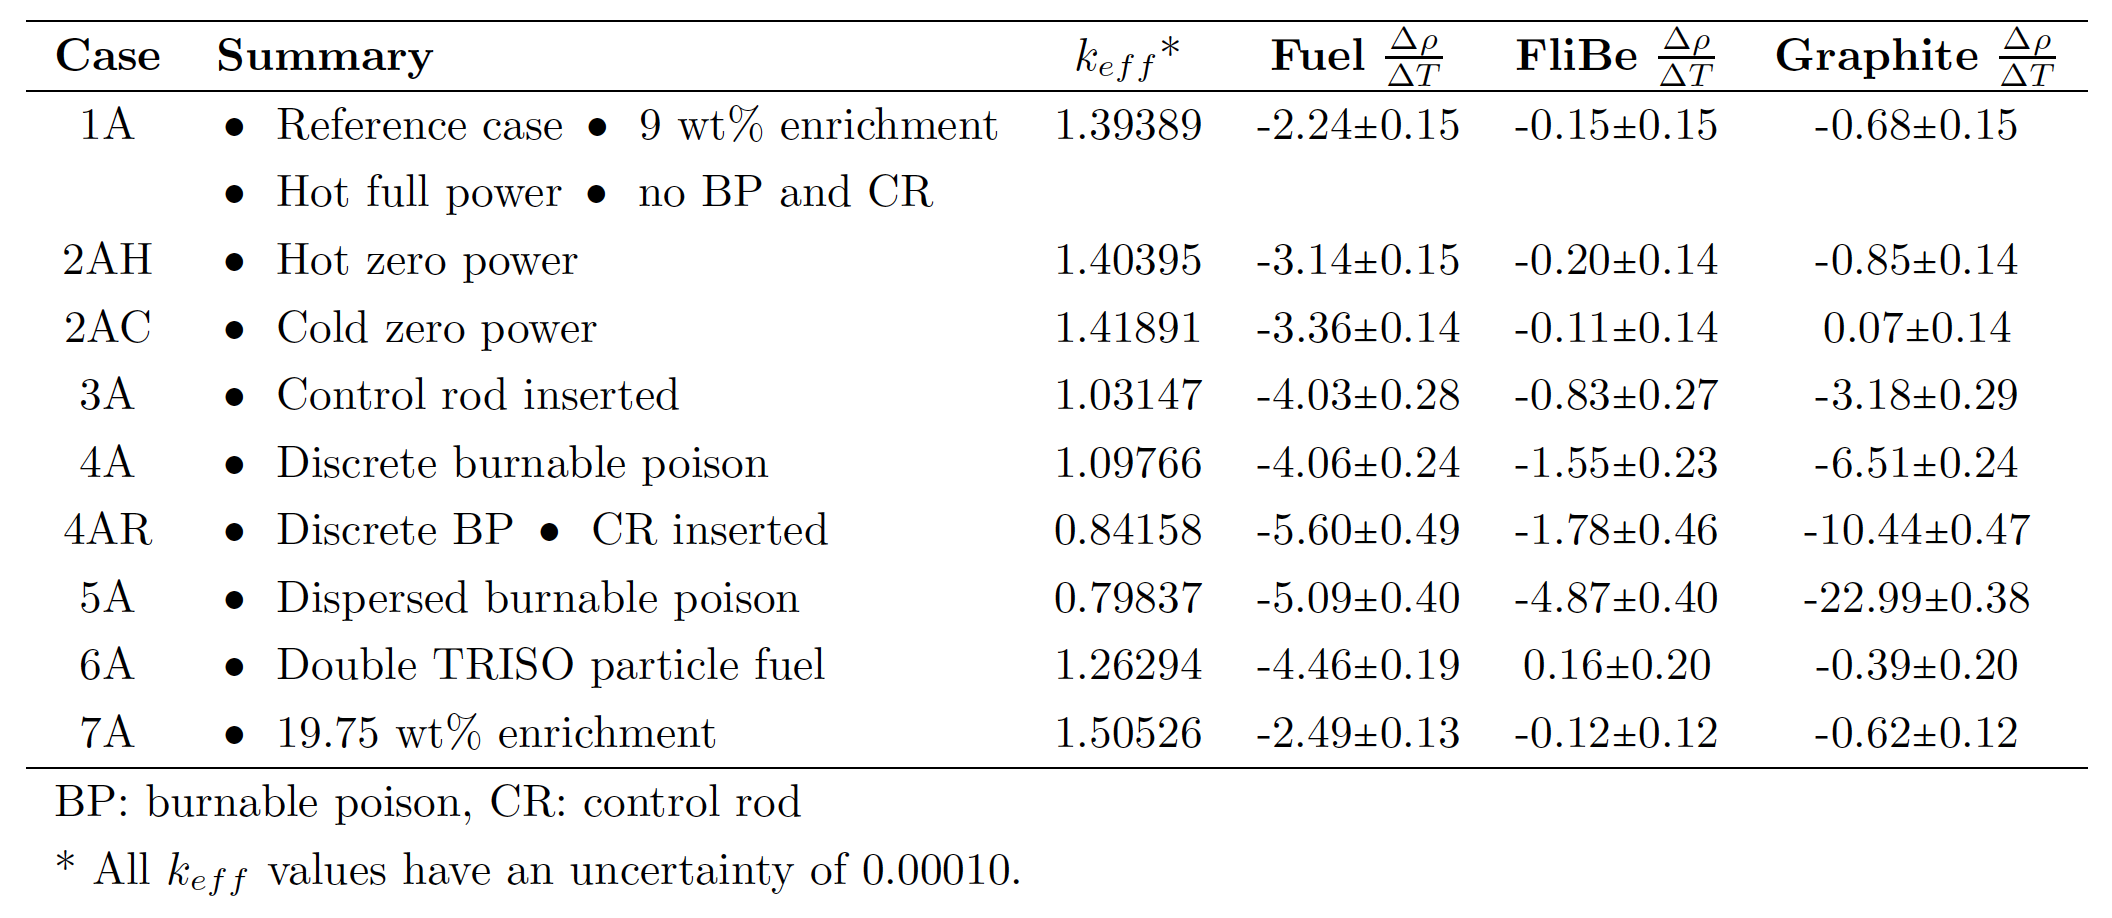
\includegraphics[width=\linewidth]{figures/benchmark-coeff-results.png}}
        \only<2>{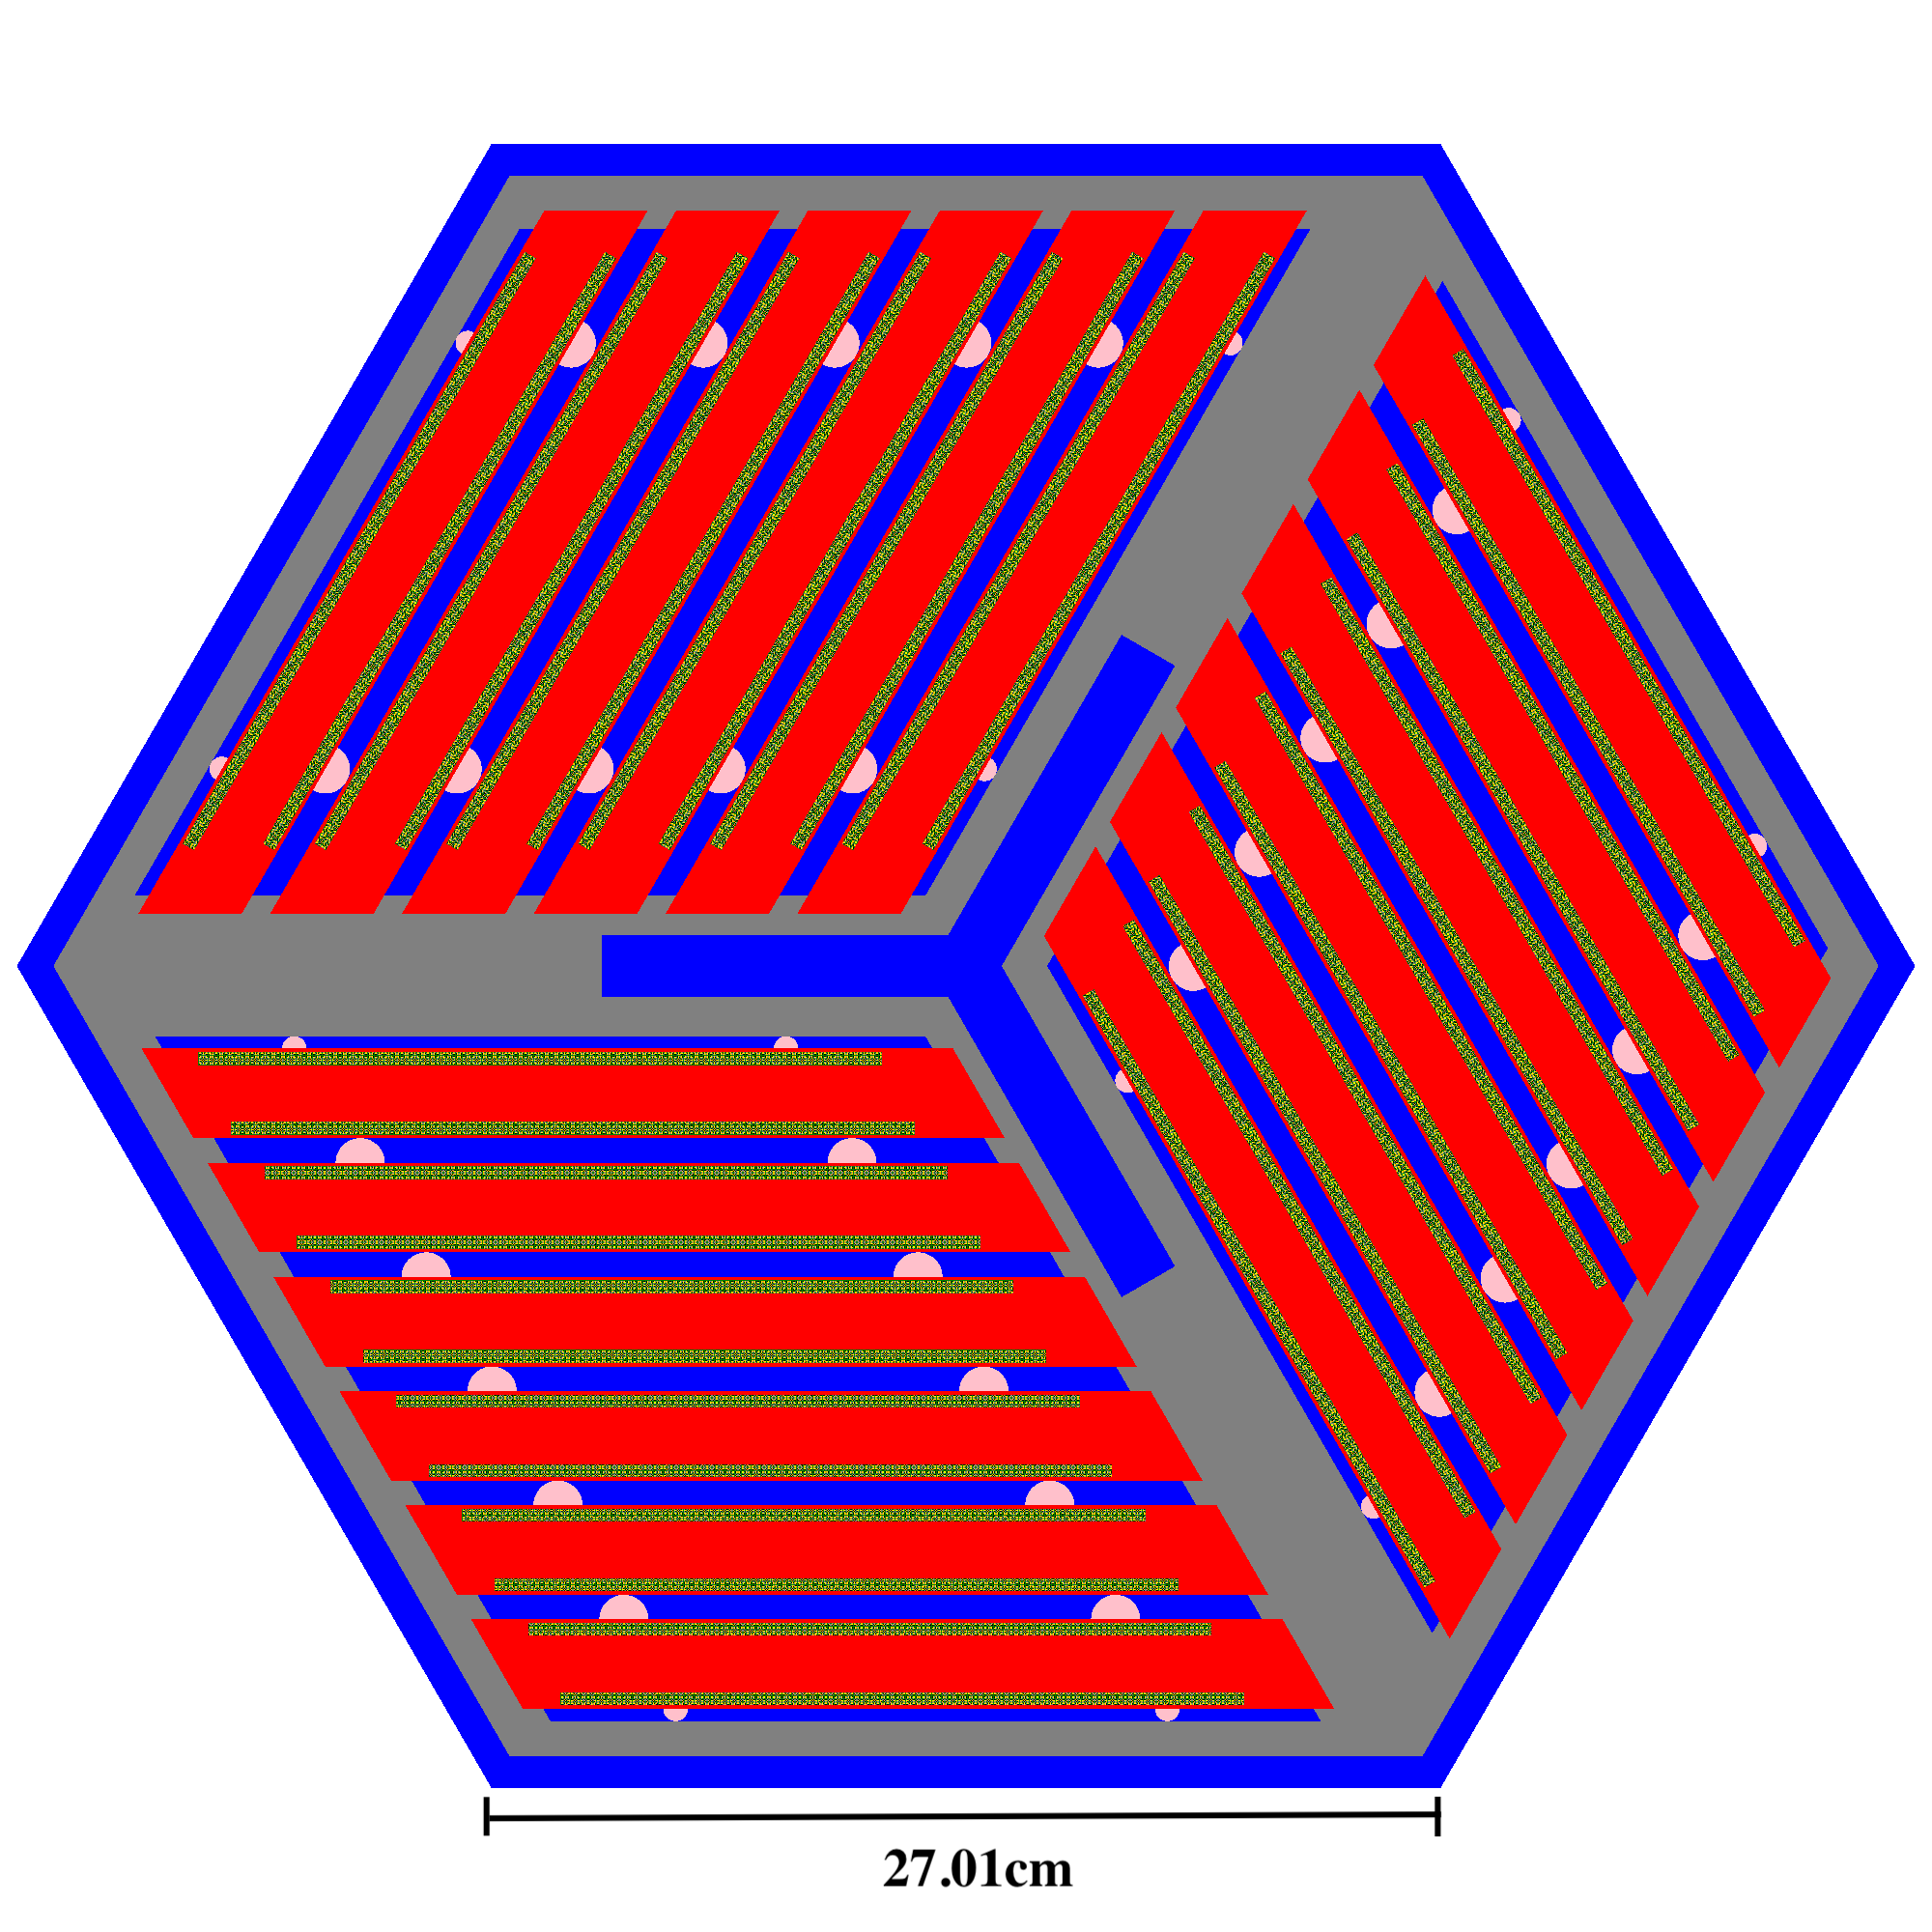
\includegraphics[width=0.6\linewidth]{../docs/figures/ahtr-fuel-element.png}}
        \only<3>{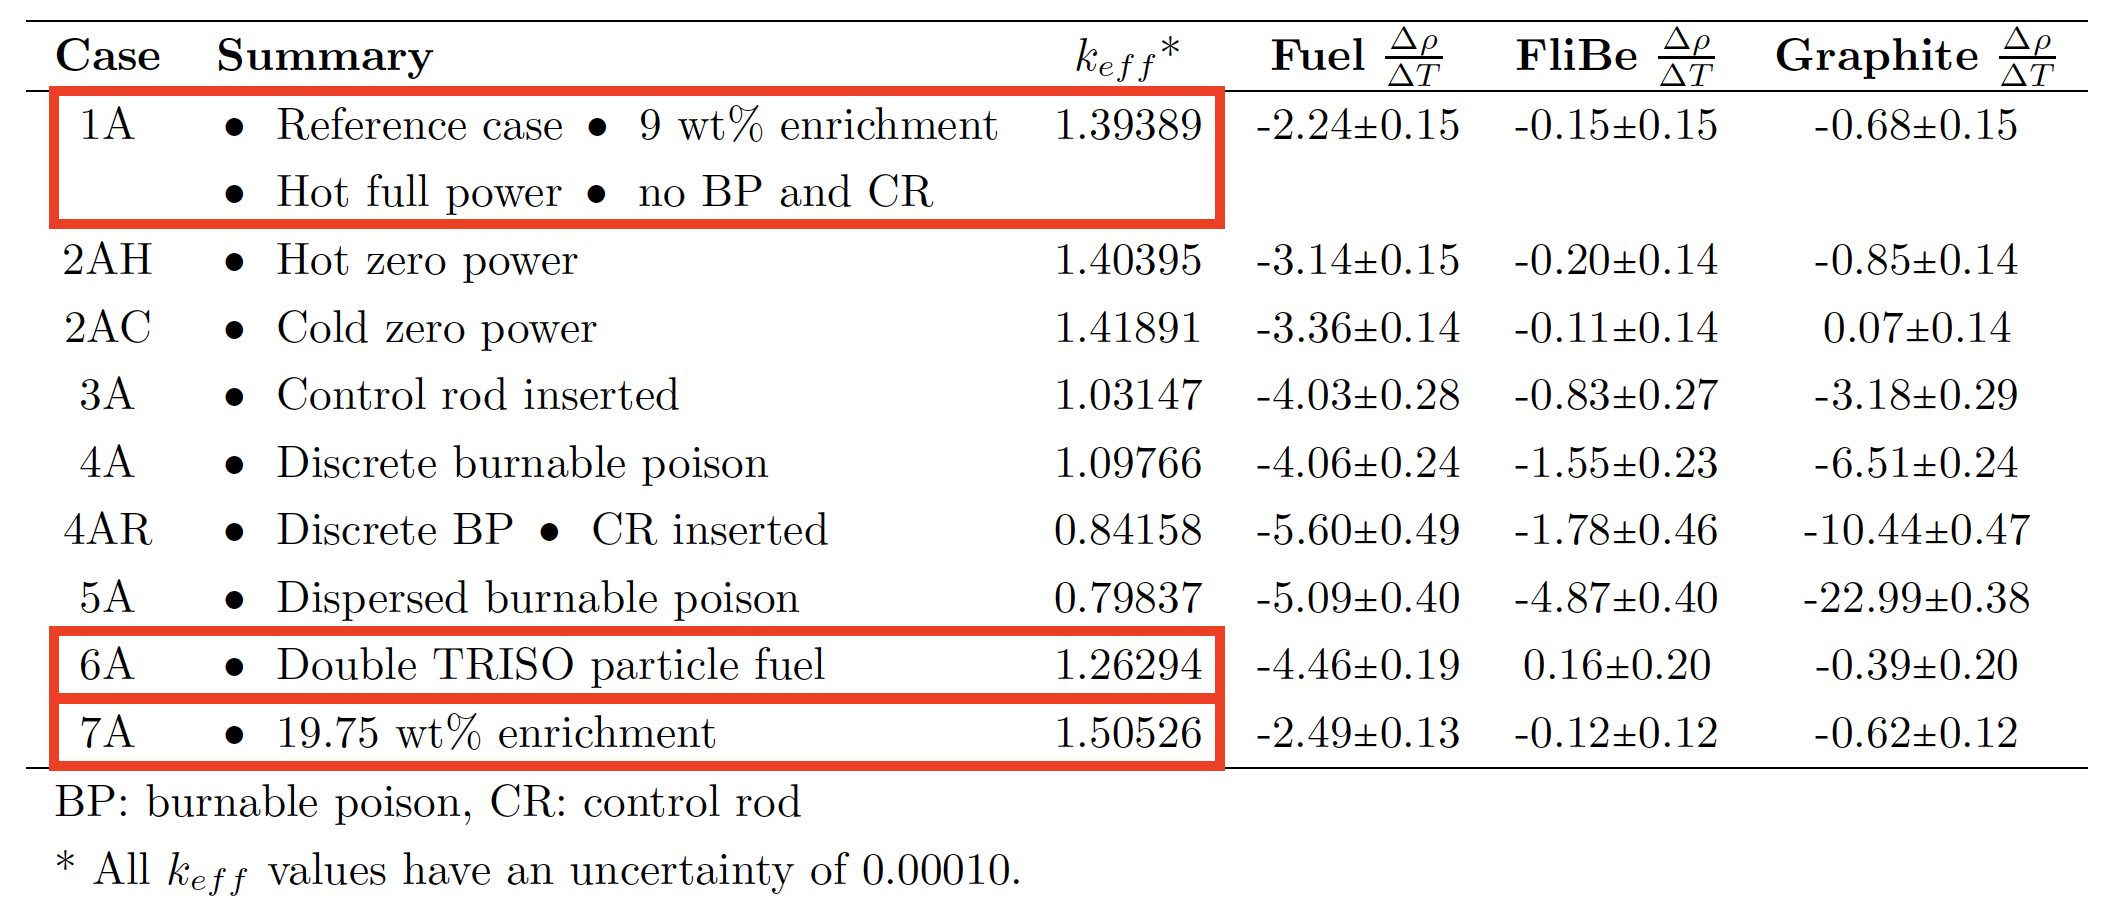
\includegraphics[width=\linewidth]{figures/benchmark-coeff-results-annotated.png}} 
        \only<4>{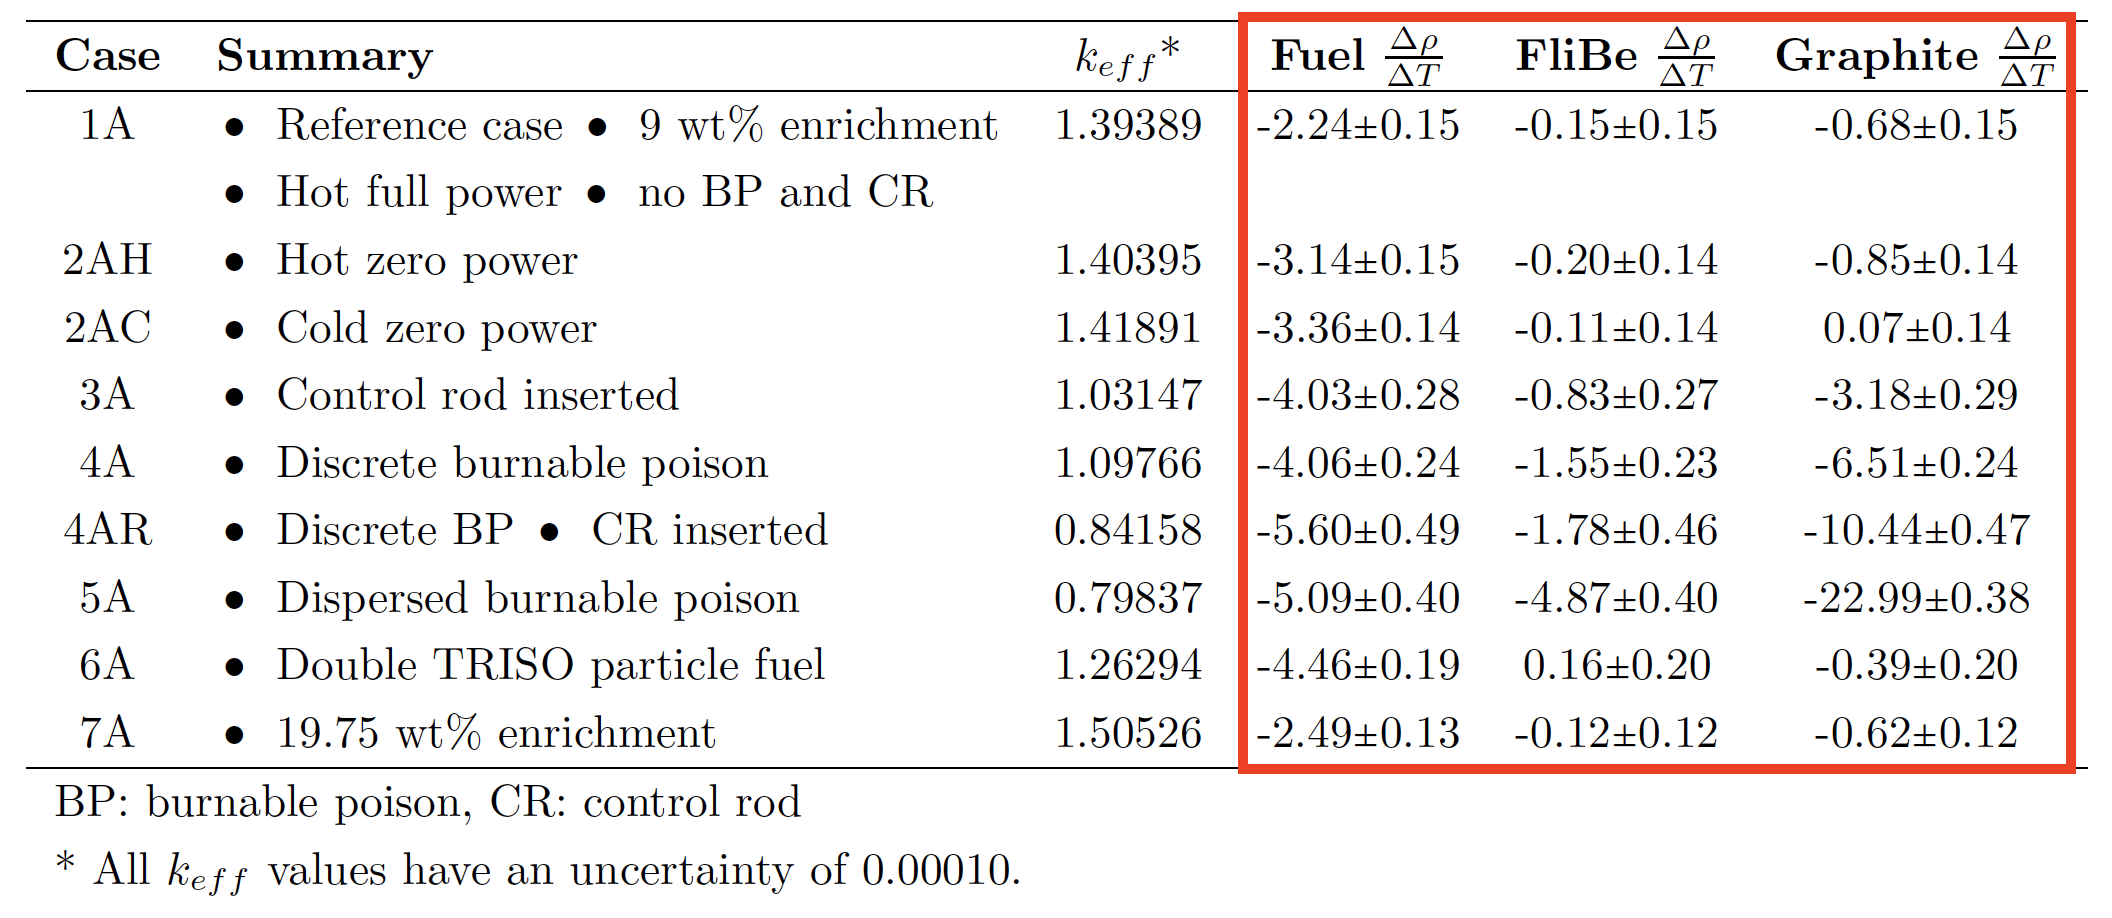
\includegraphics[width=\linewidth]{figures/benchmark-coeff-results-annotated2.png}} 
    \end{table}
    \vspace{-0.3cm}
    \only<1>{500 active cycles, 100 inactive cycles, and 200000 neutrons
    UIUC's BlueWaters supercomputer with 64 XE nodes}
    \only<3>{\textbf{Increased fuel packing does not always correspond with increased keff 
    due to spatial self-shielding effects.}}
    \only<4>{\textbf{Most of the temperature coefficients are negative, exemplifying the 
            AHTR's passive safety behavior.}}
\end{frame}

\begin{frame}
    \frametitle{FHR Benchmark Phase I-A Results}
    \vspace{-0.4cm}
    \begin{columns}
        \begin{column}{0.5\textwidth}
            \begin{figure}
                \centering
                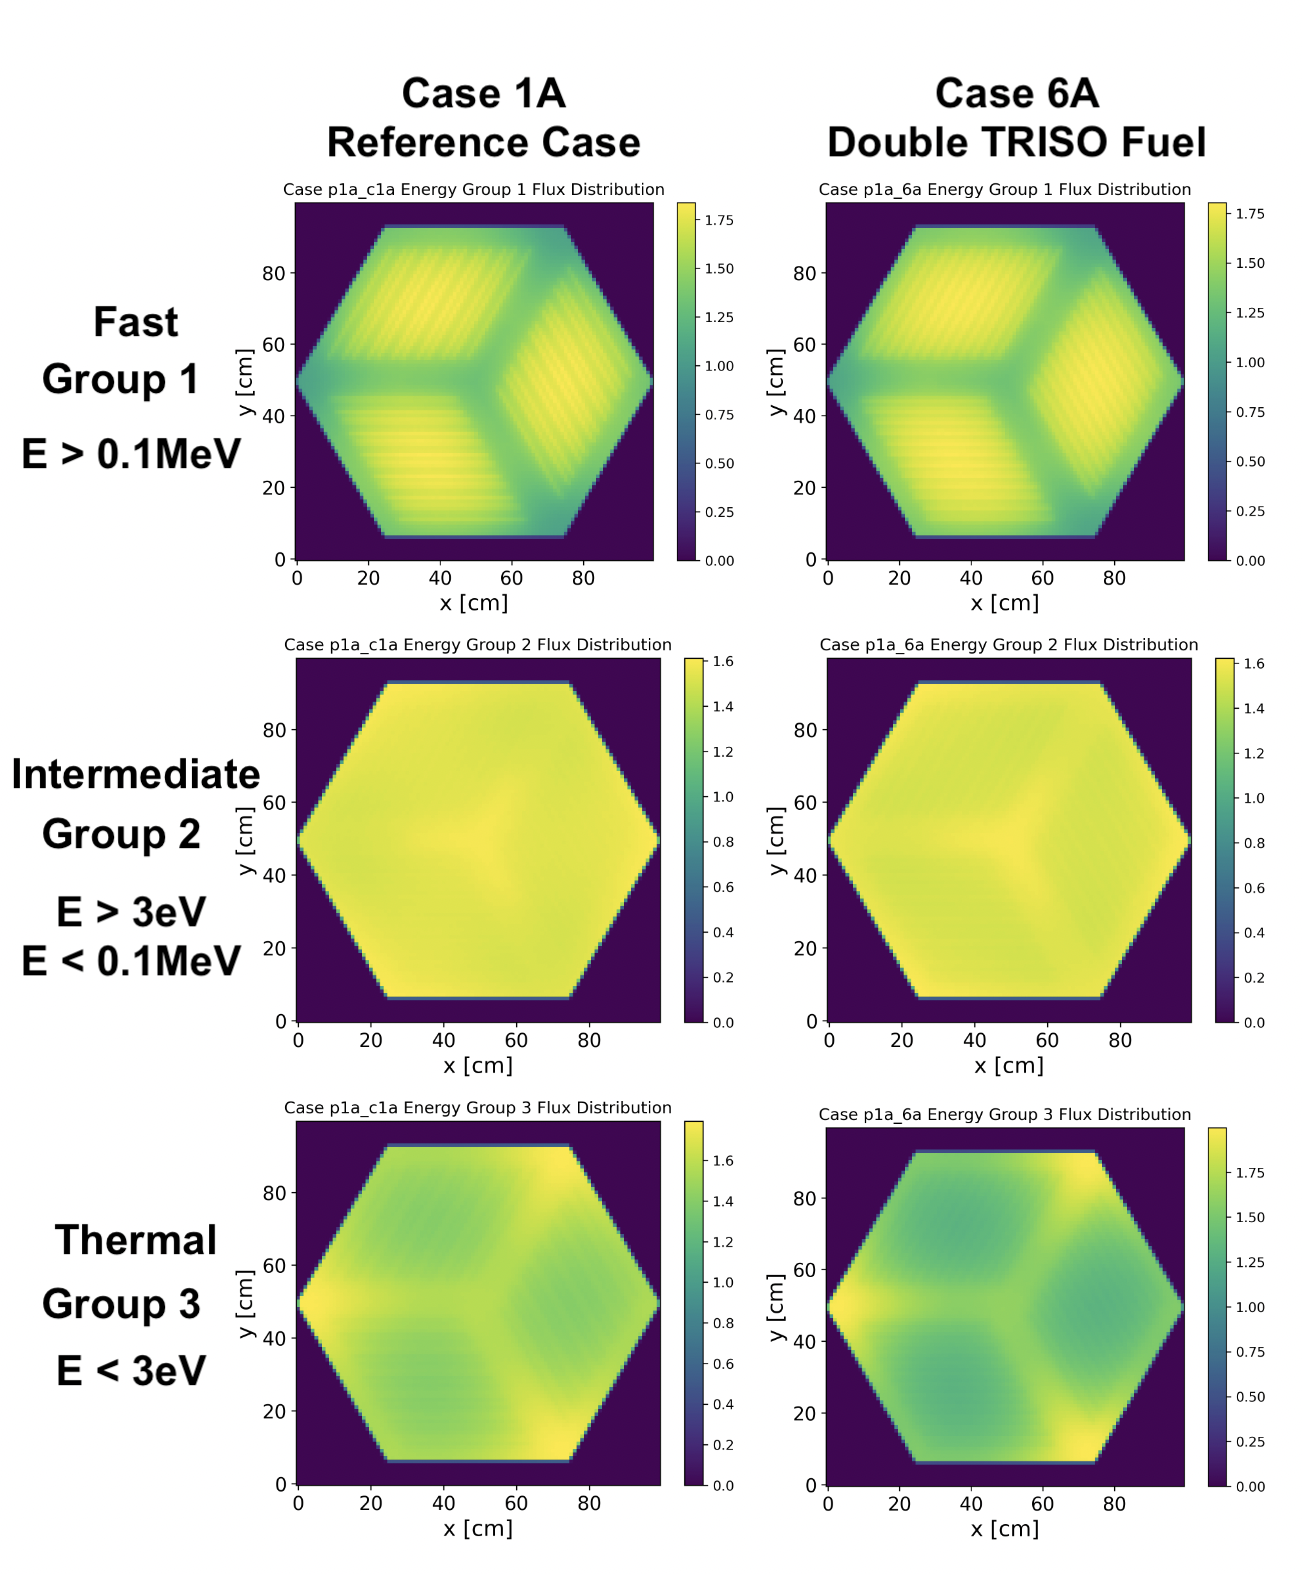
\includegraphics[width=\linewidth]{figures/phase1a-flux-vert.png} 
                \caption{Neutron flux distribution.}
            \end{figure}
        \end{column}
        \begin{column}{0.5\textwidth}
            \textbf{Key Takeaways} 
            \begin{itemize}
                \item Peak in Group 1 fast neutrons born in assembly center. Fast 
                neutrons are moderated in graphite matrix and structure 
                \item Self-shielding neutrons are more likely absorbed at the fuel 
                regions at the assembly's sides
                \item Outer sides absorb these neutrons and \textbf{geometrically 
                shield the assembly's center from neutron flux}, resulting in dip in 
                thermal Group 3 flux in the assembly's center
                \item This \textbf{self-shielding effect is more pronounced in Case 6A} 
            \end{itemize}
        \end{column}
    \end{columns}
\end{frame}

\begin{frame}
    \frametitle{FHR Benchmark Phase I-A Results}
    In an ANS M$\&$C 2021 conference paper we compared FHR benchmark participants' 
    Phase I-A results. 
    \begin{figure}[]
        \centering
        
\includegraphics[width=0.85\linewidth]{figures/mnc.png} 
        \caption{FHR benchmark paper presented at M$\&$C 2021 
        \cite{petrovic_preliminary_2021}.}
    \end{figure}

    The $k_{eff}$ standard deviation between participants for each case was in the 
    231 to 514 pcm range, \textbf{acceptable and notably close} given a blind benchmark.

    \vspace{0.2cm}
    This gives \textbf{confidence to the AHTR base model's accuracy}, as I 
    proceed to optimize the AHTR for non-conventional geometries. 
\end{frame}


\section{AHTR Moltres Model Verification and Results}
\subsection{AHTR Temperature Model with Moltres}
\begin{frame}
    \frametitle{AHTR Temperature Model}
    An AHTR temperature model captures \textbf{thermal feedback effects}, absent from 
    the purely neutronics FHR Benchmark simulations. 

    \begin{block}{Moltres \cite{lindsay_introduction_2018}}
        \begin{itemize}
			\item An application built on the \gls{MOOSE} framework, for the simulation of 
            MSRs
            \item \gls{MOOSE} \cite{gaston_moose:_2009} is an open source finite
			element framework written in \texttt{C++} that
			relies on Libmesh and PETSc for meshing and PDE solving capabilities
			\item Moltres can run transient, implicitly coupled
			neutronics/thermal-hydraulics simulations
			\begin{itemize}
				\item Multi-group neutron diffusion (arbitrary no. of groups)
				\item Delayed neutron precursor decay (with advection)
				\item Incompressible Navier-Stokes for temperature
				advection-diffusion
			\end{itemize}
		\end{itemize}
    \vspace{-0.2cm}
    \end{block}
    \begin{block}{AHTR Temperature Model with Moltres}
        \begin{itemize}
            \item I model the steady-state temperature of the AHTR full assembly's 2D 
            cross section
            \item Assumptions: conductive heat transfer, heat removal by uniform 
            salt flow in coolant regions
        \end{itemize}
    \end{block}
\end{frame}

\begin{frame}
    \frametitle{AHTR Temperature Model Setup}
    Steps to produce Moltres AHTR Temperature Model
        \begin{itemize}
          \item OpenMC neutronics model produces group constants cross-section data 
          (various macroscopic neutron cross sections, neutron diffusion coefficient, etc.)
          \item Mesh generation with Gmsh \cite{geuzaine_gmsh_2009}
          \item Run Moltres model: using these group constants and mesh, Moltres solves for the 
          flux and temperature based on the neutron diffusion equation coupled with temperature 
          advection due to coolant flow
        \end{itemize}

    \vspace{0.3cm}
    Unlike the OpenMC neutronics model, Moltres \textbf{does not explicitly model each TRISO 
    particle} because A TRISO-level fidelity mesh file is impractical and will result in an 
    extremely long Moltres runtimes. 
    
    \vspace{0.3cm}
    For successful AHTR temperature model with Moltres, I must establish 
    \textbf{suitable spatial and energy homogenization} to create group constants and mesh 
    that preserve accuracy while maintaining an acceptable runtime.
\end{frame}

\begin{frame}
    \frametitle{AHTR Temperature Model Energy Homogenization}
        \begin{table}[]
            \centering
            \caption{4-group energy structures for AHTR geometry 
            derived by Gentry et al \cite{gentry_development_2016}.}
            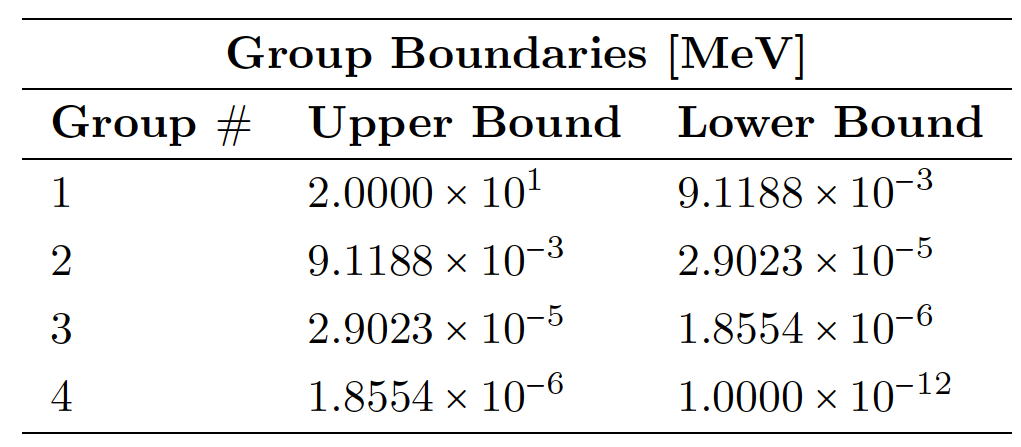
\includegraphics[width=0.6\linewidth]{figures/ahtr-energy-discr.png}
        \end{table}
\end{frame}

\begin{frame}
    \frametitle{AHTR Temperature Model Spatial Homogenization}
        \textbf{Fuel assembly 61 cell discretization}: inter-assembly FLiBe, 
        Y-shaped graphite structure, control rod slot FLiBe, graphite spacers, 
        each diamond shape section's inter-plank FLiBe (3), each graphite plank (18), 
        and each fuel stripe (36)
    \begin{figure}[]
            \centering
            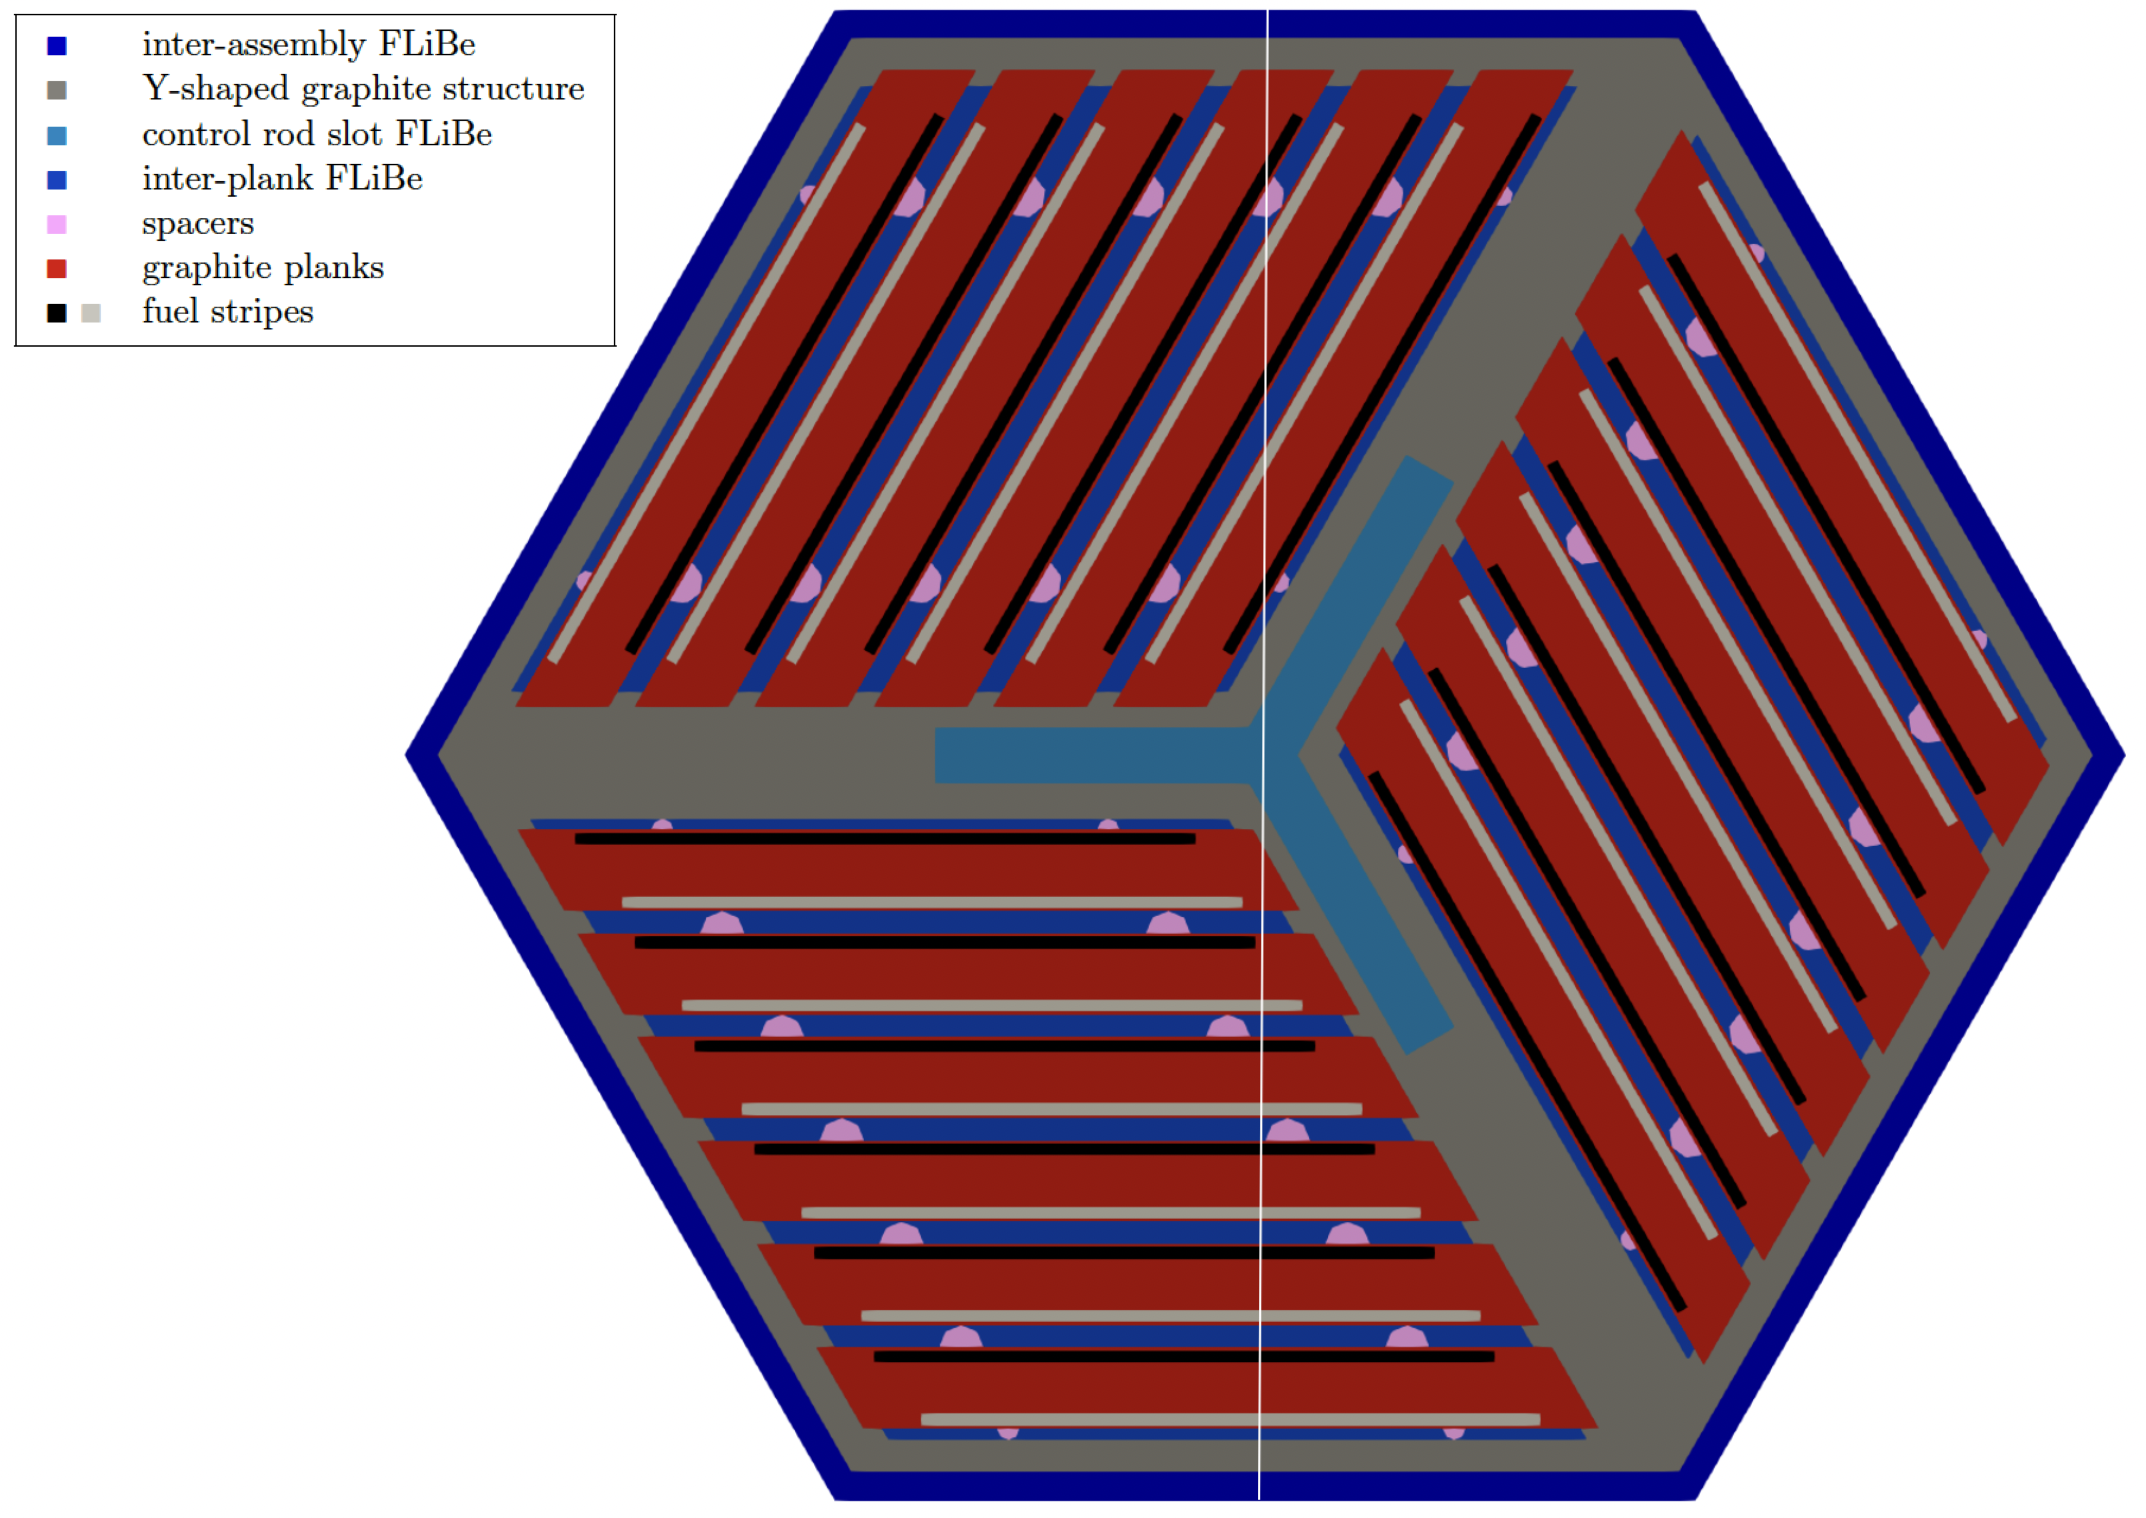
\includegraphics[width=0.65\linewidth]{figures/assembly_mg_pres.png}
        \caption{AHTR assembly spatial homogenization for group constant generation.}
    \end{figure}
\end{frame}

\subsection{Key Neutronics Parameters Verification}
\begin{frame}
    \frametitle{AHTR Temp Model Key Neutronics Parameter Verification}
    I \textbf{verify acceptable spatial homogenization and energy discretization} by 
    comparing key neutronics parameters (KNPs) between: 
    \begin{itemize} 
        \item OpenMC simulation with continuous energy and TRISO-level spatial fidelity
        \item Moltres simulation with 4-group energy and spatial homogenization
    \end{itemize}
    \textbf{KNPs}: $k_{eff}$, reactivity coefficients, flux distribution, and neutron 
    spectrum
    \begin{itemize}
        \item All comparisons are to verify that the Moltres model is replicating the 
        OpenMC model's neutronics correctly
    \end{itemize}
    \textbf{Reactivity coefficients and flux distribution}
    \begin{itemize}
        \item Ensure that \textbf{Moltres accurately calculates the AHTR's temperature 
        distribution}
        \item Reactivity coefficients capture temperature reactivity feedback on the flux
        \item Moltres source term is dependent on flux 
    \end{itemize}
\end{frame}

\begin{frame}
    \frametitle{Key Neutronics Parameter Verification Summary}
    OpenMC vs Moltres models \textbf{key observations} 
    \begin{itemize}
        \item 216 pcm reactivity difference  
        \item Good agreement in reactivity coefficients and 4-group neutron spectrum
        \item Good agreement in overall flux but larger flux diffs at specific points
    \end{itemize}
    Explanations: 
    \begin{itemize}
        \item Reactivity and flux differences due to Moltres' \textbf{neutron diffusion 
        method} 
        \item Differences in reactivity and flux at specific points might result in 
        \textbf{slightly inaccurate temperatures at certain points}
        \item Since the reactivity coefficients and overall flux distribution 
        are in agreement, this spatial homogenization and energy discretization are 
        \textbf{sufficiently accurate} to calculate and gain an \textbf{overall perspective} 
        of the AHTR's temperature distribution
    \end{itemize}
    Methodology 
    \begin{itemize}
        \item I use this same Moltres model verification method for the AHTR geometries 
        used for optimization 
    \end{itemize}
\end{frame}

\subsection{AHTR Temperature Model Results}
\begin{frame}
    \frametitle{AHTR Temperature Model Results}
    \begin{columns}
        \begin{column}{0.6\textwidth}
            \begin{figure}[]
                \centering
                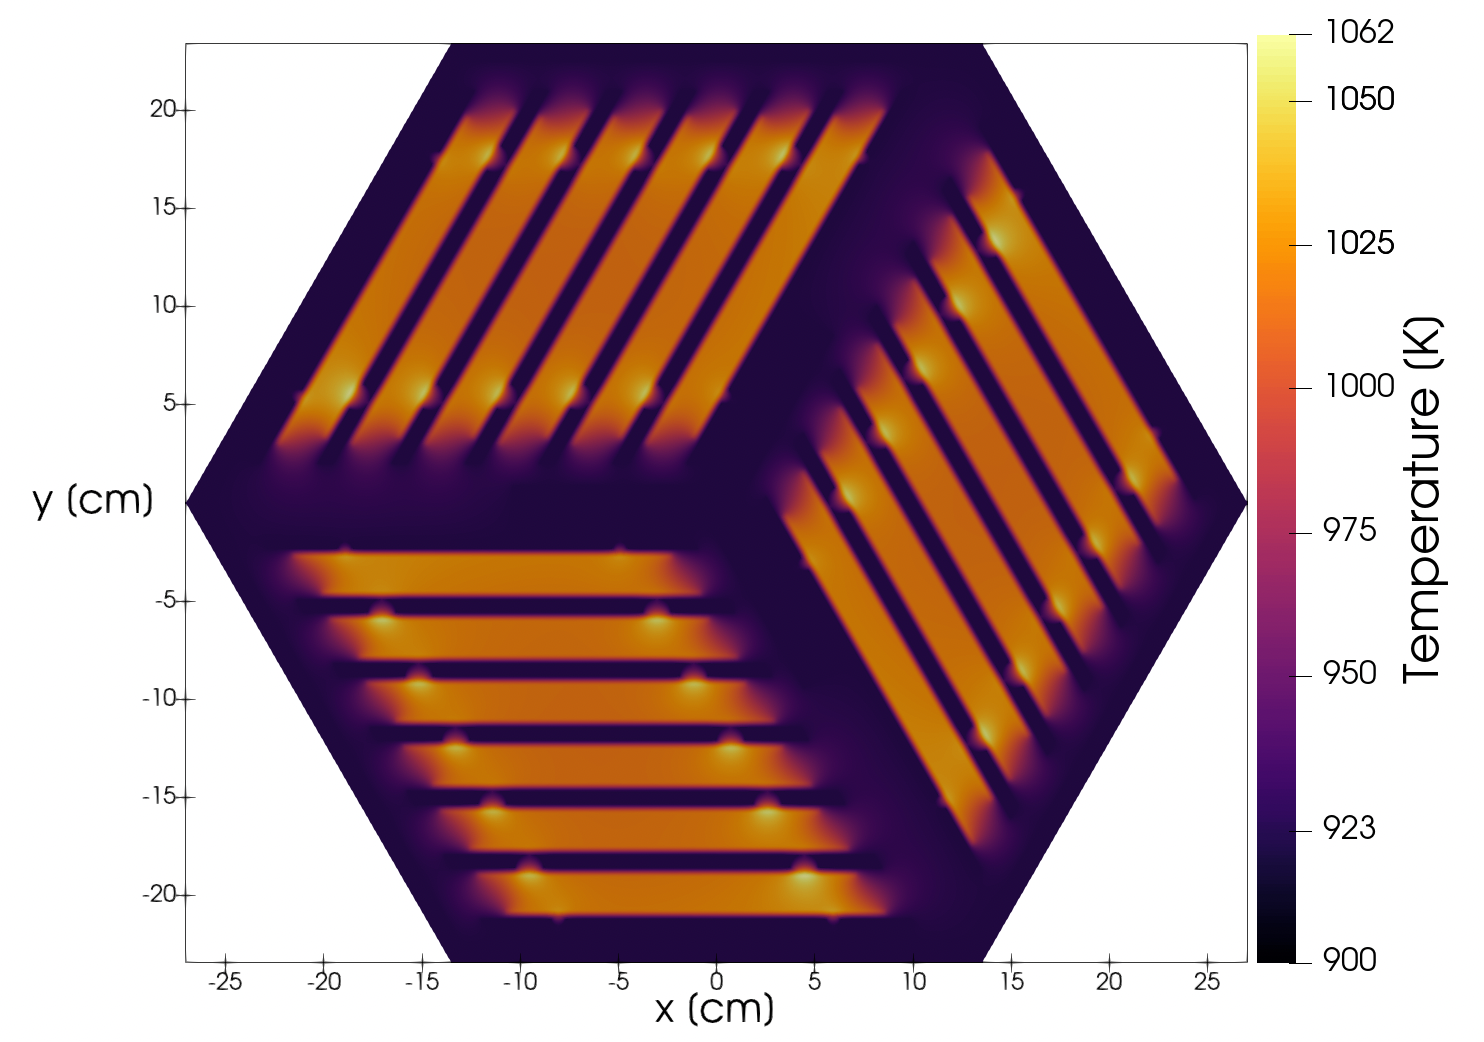
\includegraphics[width=\linewidth]{../docs/figures/benchmark-temperature-model.png} 
                \caption{2D temperature distribution in the \acrfull{AHTR}
                full assembly generated by Moltres.}
            \end{figure}
        \end{column}
        \begin{column}{0.4\textwidth} 
            \begin{block}{Results}
                \begin{itemize}
                    \item Average temperature distribution across the fuel planks are 
                    $\approx 1025K$
                    \item Average temperature of graphite structure is $\approx 935K$
                    \item Temperature peaks at 1062K in the fuel stripes near the spacers
                    \item This is due to the spacers displacing coolant and providing extra 
                    moderation 
                \end{itemize}
            \end{block}
        \end{column}
        \end{columns}
\end{frame}

\subsection{Summary}
\begin{frame}
    \frametitle{FHR Benchmark + AHTR Temperature Model: Summary}
    \begin{block}{I Successfully Completed AHTR Model Development Research Objectives}
        \begin{itemize}
            \item I participated in the OECD-NEA's FHR Benchmark Phases I-A and I-B
            \item I modeled the \gls{AHTR}'s temperature distribution with Moltres
        \end{itemize}
    \end{block}
    \begin{block}{Major Takeaways}
        \begin{itemize}
            \item AHTR has passive safety behavior with negative temperature coeffcients
            \item Increased fuel packing does not always correspond with increased 
            $k_{eff}$ due to self-shielding effects 
            \item These results hint at the possibility of \textbf{minimizing fuel required by 
            optimizing for heterogenous fuel distributions} within the core
            \item AHTR temperature peaks in the fuel stripes near the spacers 
        \end{itemize}
    \end{block}
\end{frame}


\section{ROLLO: Reactor evOLutionary aLgorithm Optimizer}
\chapter{ROLLO: Reactor evOLutionary aLgorithm Optimizer}
\label{chap:rollo}
% todo: need a nice rollo v1.0 citation
In this chapter, I introduce the \gls{ROLLO} framework developed for this dissertation. 
\gls{ROLLO} is a Python package that applies evolutionary algorithm 
techniques to optimize nuclear reactor design. 
Applying evolutionary algorithms to nuclear design problems is not new, as
discussed in Section \ref{sec:opt}. 
Reactor designers have individually customized available evolutionary algorithm 
packages for their reactor design optimization problems.
However, the evolutionary algorithm setup is highly customizable with
an assortment of genetic algorithm designs and related operators.
A reactor designer unfamiliar with evolutionary algorithms will have
to go through the cumbersome process of customizing a genetic algorithm 
for their needs and determine which operators and hyperparameters work best for 
their problem. 
Furthermore, computing fitness values with nuclear software is computationally 
expensive, necessitating using supercomputers. 
Reactor designers have to set up parallelization to use the genetic algorithm 
in concert with nuclear software.

Therefore, the motivation for \gls{ROLLO} is to limit these inconveniences and 
facilitate using evolutionary algorithms for reactor design optimization.
\gls{ROLLO} provides a general genetic algorithm framework, sets up 
parallelization for the user, and promotes usability with an input file 
that only exposes mandatory parameters.
\gls{ROLLO} strives to be effective, flexible, open-source, parallel, reproducible, 
and usable. 
I briefly summarize how \gls{ROLLO} achieves these goals:
\begin{itemize}
    \item Effective: \gls{ROLLO} is well documented and tested.
    \item Flexible: This dissertation uses \gls{ROLLO} to 
    explore arbitrary reactor geometries and heterogeneous fuel distributions. 
    However, future users might want to utilize \gls{ROLLO} 
    to explore other arbitrary design parameters. Thus, I designed the \gls{ROLLO}
    framework accordingly. The user can vary any imaginable parameter 
    because \gls{ROLLO} uses a templating method to edit the input file of the 
    coupled software.
    \item Open-source: \gls{ROLLO} is open-source and version-controlled on Github 
    \cite{chee_rollo_2021}, benefitting from the innovation of the open-source 
    community. \gls{ROLLO} also utilizes the well-documented, open-source 
    \gls{DEAP} \cite{fortin_deap_2012} Python package to drive the evolutionary 
    algorithm optimization process.
    \item Parallel: Users have the option to run \gls{ROLLO} in parallel so that 
    they may effectively use the computational resources available. 
    \item Reproducible: Data from every \gls{ROLLO} run saves into a unique, pickled 
    checkpoint file (pickle is a Python module that serializes Python objects). 
    The checkpoint file contains the \gls{ROLLO} input file and coupled evaluator's 
    scripts enabling results replication. The checkpoint file also acts as a restart 
    file for partially completed simulations. 
\end{itemize}

\gls{ROLLO} provides a framework to couple an evolutionary algorithm driver with nuclear 
software, such as neutron transport and thermal-hydraulics codes. 
\gls{ROLLO} is nuclear code-agnostic and does not have any hard dependencies on any 
nuclear software. 
Figure \ref{fig:genetic_alg} from Chapter \ref{chap:lit-review} outlined a
general evolutionary algorithm iterative problem solving process. 
I modified Figure \ref{fig:genetic_alg} to produce Figure 
\ref{fig:genetic_alg_nuclear}, which depicts how the nuclear transport and 
thermal-hydraulics software fit within \gls{ROLLO}'s evolutionary algorithm 
optimization process. 
% need to update with new algorithm style
\begin{figure}[htbp]
    \centering
    \begin{tikzpicture}[node distance=1.7cm]
            \tikzstyle{every node}=[font=\small]
            \node (1) [lbblock] {\textbf{Create initial population}};
            \node (2) [loblock, below of=1] {\textbf{Evaluate initial population}};
            \node (3) [lbblock, below of=2, yshift = -1.3cm] {\textbf{Create offspring population:} \\ 
            \begin{enumerate} \item Apply \textbf{crossover} operator to previous population
                              \item Apply \textbf{mutation} operator to previous population
                              \end{enumerate}};
            \node (4) [loblock, below of=3, yshift=-1.3cm] {\textbf{Evaluate offspring population}};
            \node (7) [lbblock, below of=4, yshift = -1.3cm] {\textbf{Create new population:} \\
            \begin{enumerate} \item Apply \textbf{selection} operator to offspring + previous population
                              \item Apply constraints to new population
                              \end{enumerate}};
            \node (5) [lbblock, below of=7, yshift=-1.3cm] {\textbf{Is termination \\ criteria satisfied?}};
            \node (6) [lbblock, below of=5] {\textbf{Best solution is returned!}};
            \draw [arrow] (1) -- (2);
            \draw [arrow] (2) -- (3);
            \draw [arrow] (3) -- (4);
            \draw [arrow] (4) -- (7);
            \draw [arrow] (7) -- (5);
            \draw [arrow] (5) -- node[anchor=east] {yes} (6);
            \draw [arrow] (5) -- ([shift={(0.5cm,0cm)}]5.east)-- node[anchor=west] {no} ([shift={(0.5cm,0cm)}]3.east)--(3);
            \matrix [draw,above right,yshift=10.7cm, xshift=0cm] at (current bounding box.south east) {
            \node [bbblock,label=right:\textbf{EA: Evolutionary Algorithm}] {}; \\
            \node [boblock,label=right:\textbf{NS: Nuclear Software}] {}; \\
            };
    \end{tikzpicture}
    \caption{Process of finding optimal solutions for a problem with a 
    genetic algorithm. Nuclear software evaluates each new population.}
    \label{fig:genetic_alg_nuclear}
\end{figure}
\gls{ROLLO} initially reads and validates the JSON input 
file, initializes the \gls{DEAP} \cite{fortin_deap_2012} genetic algorithm 
hyperparameters and operators, and finally runs the genetic algorithm following 
the flow chart in Figure \ref{fig:genetic_alg_nuclear}, in which the nuclear 
software evaluates each individual reactor model's fitness. 

The subsequent sections describe \gls{ROLLO}'s evolutionary algorithm driver 
software \gls{DEAP} (Section \ref{sec:rollo-ea}), input file structure (Section 
\ref{sec:rollo-input-file}), software architecture (Section \ref{sec:rollo-archi}), 
verification studies (Section \ref{sec:rollo-verification}), and convergence criteria
(Section \ref{sec:rollo-convergence}). 
Appendix B lists all the data and analysis related to this chapter to enable the 
reproduction of all the simulations.

\section{Evolutionary Algorithm Driver}
\label{sec:rollo-ea}
Evolutionary algorithm computation uses sophisticated, diverse techniques 
and mechanisms, resulting in even the most well-designed software frameworks 
being complicated under the hood. 
Utilizing an existing evolutionary algorithm framework presents implementation 
challenges as the user must edit the framework's source code to customize it for their 
application and hyperparameters \cite{fortin_deap_2012}. 
Therefore, a computation framework that gives the user the capability to build 
custom evolutionary algorithms is ideal for this project.

Many evolutionary algorithm computation packages exist: 
\gls{DEAP} \cite{fortin_deap_2012}, Pymoo \cite{blank_pymoo_2020}, inspyred 
\cite{garrett_inspyred_2014}, Pyevolve \cite{perone_pyevolve_2009}, and 
OpenBEAGLE \cite{gagne_open_2002}.
\gls{DEAP} is the newest package and places a high value on code 
compactness and clarity \cite{fortin_deap_2012}. 
\gls{DEAP} is the only framework that allows the user to prototype evolutionary 
algorithms rapidly and define custom algorithms without digging deep into 
the source code to modify hyperparameters and their application methods.
Accordingly, I chose \gls{DEAP} to drive the \gls{ROLLO} framework's 
evolutionary algorithm component. 
\gls{DEAP} provides building blocks for each optimizer function and allows the 
user to customize a specialized algorithm to fit their project \cite{fortin_deap_2012}.

\subsection{Distributed Evolutionary Algorithms in Python}
\label{sec:deap-works}
\gls{DEAP} is composed of two structures: a \textit{creator} and a 
\textit{toolbox}.  
The \textit{creator} module allows the run-time creation of classes via 
inheritance and composition, enabling individual and population creation 
from any data structure: lists, sets, dictionaries, trees, etc \cite{fortin_deap_2012}. 
The \textit{toolbox} is a container that the user manually populates.
In the \textit{toolbox}, the user defines the selection, crossover, and 
mutation operator types and their respective hyperparameters.
For example, the user registers a crossover operator under the `mate'
alias and a selection operator under the `select' alias. 
Then, the evolutionary algorithm uses these aliased operators from the 
\textit{toolbox}. 
If the user wants to change the crossover operator, they update the 
`mate' alias in the \textit{toolbox} while keeping the evolutionary algorithm 
unchanged \cite{fortin_deap_2012}. 

Figure \ref{fig:deap-code} illustrates \gls{DEAP}'s usage of the \textit{creator} and
\textit{toolbox} modules. 
\begin{figure}[htbp]
    \begin{minted}[
        frame=lines,
        framesep=2mm,
        baselinestretch=1.2,
        fontsize=\footnotesize,
        linenos
        ]{python}
        
        from deap import creator, base, tools, algorithms
        creator.create("Objective", base.Fitness, weights=(-1.0,)) # minimum
        creator.create("Individual", list, fitness=creator.Objective)

        toolbox = base.Toolbox()
        toolbox.register("variable_1", random.uniform, 0.0, 10.0)
        toolbox.register("variable_2", random.uniform, -1.0, 0.0)
        def individual_creator():
            return creator.Individual([toolbox.variable_1(), toolbox.variable_2()])
        toolbox.register("individual", individual_creator())
        toolbox.register("population", tools.initRepeat, list, toolbox.individual)
        def evaluator_fn(individual):
            return tuple([sum(individual)])
        toolbox.register("evaluate", evaluator_fn)
        toolbox.register("select", tools.selBest, k=5)
        toolbox.register("mutate", tools.mutPolynomialBounded, eta=0.5, low=[0, -1], up=[-1, 0])
        toolbox.register("mate", tools.cxOnePoint)
    \end{minted}
    \caption{DEAP sample code demonstrating the usage of the \textit{creator} and
    \textit{toolbox} modules to initialize the genetic algorithm. In \gls{ROLLO}, \gls{DEAP}'s 
    \textit{creator} and \textit{toolbox} modules are initialized in the source 
    code based on the genetic algorithm parameters defined by the user in the 
    \gls{ROLLO} input file. }
    \label{fig:deap-code}
\end{figure}
Line 2 creates a single-objective fitness class, \texttt{Objective}. 
The first argument defines the derived class's name; the second argument 
specifies the inherited base class, \texttt{base.fitness}; the third 
argument indicates the objective fitness ($-1.0$ indicates a minimum objective, 
$+1.0$ indicates a maximum objective). 
Line 3 derives an \texttt{Individual} class from the standard Python list type
and defines its fitness attribute as the newly created \texttt{Objective} object. 
Lines 5-9 initialize the \gls{DEAP} toolbox, register 
\texttt{variable\_1} and \texttt{variable\_2} with their upper and lower bounds, 
and defines the \texttt{individual\_creator} function to return an 
\texttt{Individual} initialized with \texttt{variable\_1} and \texttt{variable\_2}. 
Lines 10-11 and 14-17 are aliases for initializing individuals and populations, 
specifying variation operators (\texttt{select}, \texttt{mutate}, \texttt{mate}), 
and evaluating individual fitness (\texttt{evaluate}) \cite{fortin_deap_2012}. 
Lines 12-13 define the evaluation function that returns the fitness values. 

\gls{ROLLO} initializes \gls{DEAP}'s \textit{creator} and \textit{toolbox} modules 
based on the genetic algorithm parameters defined by the user in the \gls{ROLLO} 
input file. 
The evaluation function runs the nuclear software and returns user-defined 
fitness values. 

\subsection{ROLLO Evolutionary Algorithm Implementation}
\gls{DEAP} creators provided variations of a classical genetic algorithm 
exposing different explicitness levels \cite{fortin_deap_2012}. 
The high-level examples use the built-in \gls{DEAP} genetic algorithms, 
whereas the low-level example completely unpacks the genetic algorithm to expose 
a generational loop. 
I included an unpacked genetic algorithm in ROLLO's 
\textbf{\textit{Algorithm}} class, depicted in Figure \ref{fig:genetic_alg_nuclear}. 
The algorithm begins by initializing the starting population and evaluating 
each individual's fitness value. 
Then, it enters a generational loop. 
During each iteration, the mating and mutation operators are applied to the population
to create an offspring population, and all offspring individuals are evaluated. 
The selection operator is then applied to both the previous and offspring populations 
to select the best individuals to create the new population. 
Finally, the constraints are applied, and the results are saved.
Applying the selection operator to the combined previous and offspring 
populations expands the population, ensuring the effectiveness of 
elitism selection operators, such as NSGA-II, which work well 
for multiobjective optimization. 

\section{ROLLO Input File}
\label{sec:rollo-input-file}
\gls{ROLLO}'s input file is in JSON format. 
There are four sections that the user must define: \\ \texttt{control\_variables}, 
\texttt{evaluators}, \texttt{constraints}, and \texttt{algorithm}. 
Figure \ref{fig:rollo-input} shows an example \gls{ROLLO} input file. 
In this example, \gls{ROLLO} uses a genetic algorithm with user-defined 
hyperparameters, defined in the \texttt{algorithm} secion, to minimize the 
\texttt{output1} parameter.
The OpenMC evaluator accepts input parameters: \texttt{variable1} and 
\texttt{variable2}, and calculates the \texttt{output1} parameter.
\begin{figure}[htbp]
    \begin{minted}[
        frame=lines,
        framesep=2mm,
        baselinestretch=1.2,
        fontsize=\footnotesize,
        linenos
        ]{json}
        {
            "control_variables": {
                "variable1": {"min": 0.0, "max": 10.0}, 
                "variable2": {"min": -1.0, "max": 0.0}
            }, 
            "evaluators": {
                "openmc": {
                    "order": 0,
                    "inputs": ["variable1", "variable2"],
                    "input_script": ["python", "openmc_inp.py"],
                    "execute": [["openmc"],],
                    "outputs": ["output1", "output2"]
                    "output_script": ["python", "openmc_output.py"], 
                }
            }, 
            "constraints": {
                "output1": {"operator": [">=", "<"], "constrained_val": [1.0, 1.5]}
            }, 
            "algorithm": {
                "objective": ["min"], 
                "weight": [1.0],
                "optimized_variable": ["output1"], 
                "pop_size": 100, 
                "generations": 10, 
                "parallel": "job_control",
                "keep_files": "all",
                "mutation_probability": 0.23,
                "mating_probability": 0.46,
                "selection_operator": {"operator": "selTournament", "tournsize":5},
                "mutation_operator": {
                    "operator": "mutPolynomialBounded",
                    "indpb": 0.23,
                    "eta": 0.23
                },
                "mating_operator": {"operator": "cxBlend", "alpha": 0.46}
            }
        }
    \end{minted}
    \caption{\acrfull{ROLLO} sample JSON input file.}
    \label{fig:rollo-input}
\end{figure}
Next, I describe how to define each section of a \gls{ROLLO} input file. 
The \gls{ROLLO} documentation \cite{chee_documentation_2021} provides further 
descriptions for setting up a \gls{ROLLO} input file.

\subsection{Control Variables}
I use the term control variables to refer to parameters the genetic algorithm will 
vary (conventionally, a control variable is held constant in a research study 
however this is not the case for \gls{ROLLO}).
The user must specify the minimum and maximum values for each control variable.
For example, Lines 2 to 5 in Figure \ref{fig:rollo-input} demonstrate that the 
control variables, \texttt{variable1} and \texttt{variable2}, 
will be varied from 0 to 10 and -1 to 0, respectively. 
For example, in traditional reactor design, a control variable might be fuel 
enrichment. 

\subsection{Evaluators}
Evaluators are the nuclear software \gls{ROLLO} utilizes to calculate objective functions. 
\gls{ROLLO} is nuclear code-agnostic and does not have hard dependencies on any 
nuclear software.
Thus, it is up to the user to ensure that the nuclear software and their corresponding 
executables are correctly installed. 
In a single \gls{ROLLO} input file, users may define any number of evaluators. 
For each evaluator, mandatory parameters are \texttt{order}, \texttt{input\_script}, 
\texttt{inputs}, and \texttt{outputs}, and the optional parameters are
\texttt{execute} and \texttt{output\_script}. 
Table \ref{tab:evaluator-inputs} describes each evaluator's mandatory and optional parameters 
in the \gls{ROLLO} \texttt{evaluators}' input file section.  
\begin{table}[htbp]
    \centering
    \onehalfspacing
    \caption{\acrfull{ROLLO} \texttt{evaluator}: Input Parameter Descriptions.}
	\label{tab:evaluator-inputs}
    \footnotesize
    \begin{tabular}{l|lp{2.5cm}p{7cm}}
    \hline
    & \textbf{Parameter} & \textbf{Type} & \textbf{Description} \\
    \hline
    \multirow{9}{2cm}{Mandatory Parameters} & \texttt{order} & int 
    & evaluator's operational order compared to other evaluators (indexed by 0) \\
    \cline{2-4}
    & \texttt{inputs} & list of strings & control variables to be placed in the input 
    script template \\
    \cline{2-4}
    & \texttt{input\_script} & list of strings (2-element) & 1st element: executable to 
    run input script, 2nd element: input script template \\
    \cline{2-4}
    & \texttt{outputs} & list of strings & output variables that the evaluator will return to the genetic algorithm \\
    \hline
    \multirow{4}{2cm}{Optional Parameters} & \texttt{execute} & list of 2-element lists &
    enables users to run other executables or files beyond the input and output scripts. 
    1st element: executable to run file, 2nd element: file to run \\
    \cline{2-4}
    & \texttt{output\_script} & list of strings (2-element) & 1st element: executable to 
    run output script, 2nd element: output script template \\
    \hline 
    \end{tabular}
    \end{table}

\gls{ROLLO} utilizes jinja2 templating \cite{ronacher_welcome_2018} to insert 
the control variable values into the \texttt{input\_script}.
Users must include each evaluator's input file template in the same directory as the \gls{ROLLO} input 
file. 
Users must also ensure the template variables correspond to the \texttt{inputs} defined in the 
corresponding evaluator's section in the ROLLO input file. 
Lines 6 to 13 in the \gls{ROLLO} input file (Figure \ref{fig:rollo-input}) demonstrate 
that \texttt{variable1} and \texttt{variable2} are \texttt{inputs} into the 
\texttt{openmc\_inp.py} \texttt{input\_script}. 
Figure \ref{fig:openmcinp.py} shows the template and templated openmc script; 
once the \texttt{openmc\_inp.py} \texttt{input\_script} is templated, 
\texttt{\{\{variable1\}\}} and \texttt{\{\{variable2\}\}}  on Lines 3 and 4 will be 
replaced with values selected by the \gls{ROLLO} genetic algorithm. 
\begin{figure}[htbp]
    \begin{minipage}{0.4\textwidth}
        \centering
    \begin{minted}[
        frame=lines,
        framesep=2mm,
        baselinestretch=1.2,
        fontsize=\footnotesize,
        linenos
        ]{python}
        import openmc 
        # templating 
        variable1 = {{variable1}}
        variable2 = {{variable2}}
        # run openmc 
        ... 
    \end{minted}
    \end{minipage}
    \hspace{2cm}
    \begin{minipage}{0.4\textwidth}
        \centering
        \begin{minted}[
            frame=lines,
            framesep=2mm,
            baselinestretch=1.2,
            fontsize=\footnotesize,
            linenos
            ]{python}
            import openmc 
            # templating 
            variable1 = 3.212
            variable2 = -0.765
            # run openmc 
            ... 
        \end{minted}
        \end{minipage}
    \caption{\texttt{openmc\_inp.py} input script template (left). 
             Templated \texttt{openmc\_inp.py} with variable1 and variable2 
             values defined (right).}
    \label{fig:openmcinp.py}
\end{figure}

\gls{ROLLO} uses two methods to return an output variable to the genetic algorithm. 
First, \gls{ROLLO} will automatically return the input parameter's value if the output 
parameter is also an input parameter. 
Second, the user may include an \texttt{output\_script} that returns the desired 
output parameter. 
The \texttt{output\_script} must include a line that prints a dictionary containing 
the output parameters' names and their corresponding value as key-value pairs. 

\subsection{Constraints}
In the constraints section, the user can define constraints on any output parameter. 
Any individual that does not meet the defined constraints is removed from the 
population, encouraging the proliferation of individuals that meet the 
constraints. 
For each constrained output parameter, the user lists the \texttt{operator}s 
and \texttt{constrained\_val}s as in Line 17 of the \gls{ROLLO} input file 
(Figure \ref{fig:rollo-input}). 
Thus, for this \gls{ROLLO} simulation, \texttt{output\_1} is constrained to be 
$>= 1.0$ and $< 1.5$. 
For example, for reactor safety, a constraint might be the maximum temperature in the 
core.

\subsection{Algorithm}
In the algorithm section, users define the simulation's general settings and the
genetic algorithm's hyperparameters. 
The mandatory input parameters include \texttt{optimized\_variable}, \texttt{objective},
\texttt{pop\_size}, and \texttt{generations}.
The optional input parameters include \texttt{parallel}, \texttt{keep\_files}, \\
\texttt{mutation\_probability}, \texttt{mating\_probability}, 
\texttt{selection\_operator}, \texttt{mutation\_operator}, 
and \texttt{mating\_operator}. 
Lines 17 to 31 in the example \gls{ROLLO} input file (Figure \ref{fig:rollo-input}) 
demonstrate \texttt{algorithm} specifications. 
Table \ref{tab:algorithm-inputs} describes these input parameters in detail. 
\begin{table}[htbp]
    \centering
    \onehalfspacing
    \caption{\acrfull{ROLLO} \texttt{algorithm}: Input Parameter Descriptions.}
	\label{tab:algorithm-inputs}
    \scriptsize
    \begin{tabular}{l|lp{1.5cm}p{3.7cm}p{3.5cm}}
    \hline
    & \textbf{Parameter} & \textbf{Type} & \textbf{Description} & \textbf{Default} \\
    \hline
    \multirow{9}{1.8cm}{Mandatory Parameters} 
    & \texttt{optimized\_variable} & list of strings & variables to be optimized & -\\
    \cline{2-5}
    & \texttt{objective} & list of strings & options include: min or max,
    each objective corresponds to a variable in \texttt{optimized\_variable} & -\\
    \cline{2-5}
    & \texttt{pop\_size} & int & population size & -\\
    \cline{2-5}
    & \texttt{generations} & int & number of generations & -\\
    \hline
    \multirow{15}{1.8cm}{Optional Parameters} 
    & \texttt{parallel} & string & options include: \textit{none}, \textit{multiprocessing}, \textit{job\_control} & \textit{none} \\
    \cline{2-5}
    & \texttt{keep\_files} & string & options include: \textit{none}, \textit{only\_final}, \textit{all} & \textit{none} \\
    \cline{2-5}
    & \texttt{mutation\_probability} & float & mutation probability & 0.23 \\
    \cline{2-5}
    & \texttt{mating\_probability} & float & mating probability & 0.47 \\
    \cline{2-5}
    & \texttt{selection\_operator} & dict & see Table \ref{tab:deap_operators} & \scriptsize{{"operator": "selTournament", "tournsize": 5}}\\
    \cline{2-5}
    & \texttt{mutation\_operator} & dict & see Table \ref{tab:deap_operators} & \scriptsize{{"operator": "mutPolynomialBounded", "eta": 0.23, "indpb": 0.23}}\\
    \cline{2-5}
    & \texttt{mating\_operator} & dict & see Table \ref{tab:deap_operators} & \scriptsize{{"operator": "cxBlend", "alpha": 0.46}}\\
    \hline 
    \end{tabular}
    \end{table}
The hyperparameter default values are selected based on hyperparameter studies conducted 
for a single objective \gls{FHR} optimization. 
Section \ref{sec:hyperparameter-studies} describes the hyperparameter studies. 

As mentioned previously in Section \ref{sec:genetic_alg}, it is important to 
select genetic algorithm hyperparameters that balance the extent of exploration 
and exploitation.
% todo: add this phrasing earlier in chapter too. 
For each operator, users choose from a list of operators and define each
of their required hyperparameters. 
Table \ref{tab:deap_operators} shows the available operators and their respective 
hyperparameters. 
Descriptions for each operator can be found in Section \ref{sec:genetic_alg}.
\begin{table}[htbp]
    \centering
    \onehalfspacing
    \caption{Selection, mutation, and mating operators available in 
    \acrfull{ROLLO} and their corresponding hyperparameters. n/a indicates that 
    the operator does not have associated hyperparameters. }
	\label{tab:deap_operators}
    \footnotesize
    \begin{tabular}{l|p{0.23\textwidth}|p{0.55\textwidth}}
    \hline
    \textbf{Operator} & \textbf{Available Options} & \textbf{Hyperparameters} \\ \hline
    \multirow{4}{1cm}{Selection} & \texttt{selTournament} & \texttt{tournsize}: no. of individuals in each tournament\\ \cline{2-3}
    & \texttt{selNSGA2} & n/a \\ \cline{2-3}
    & \texttt{selBest} & n/a \\ \hline
    \multirow{2}{1cm}{Mutation} & \multirow{2}{2cm}{\texttt{mutPolynomialBounded}} & \texttt{eta}: crowding degree of the mutation\\  
    && \texttt{indpb}: independent probability for each attribute to be mutated\\ \hline
    \multirow{3}{1cm}{Mating} & \texttt{cxOnePoint} & n/a \\ \cline{2-3}
    & \texttt{cxUniform} & \texttt{indpb}: independent probability for each attribute to be exchanged\\ \cline{2-3}
    & \texttt{cxBlend} & \texttt{alpha}: Extent of the interval that the new values can be drawn for each attribute on both sides of the parents’ attributes\\ \hline
    \end{tabular}
    \end{table}

\section{ROLLO Software Architecture}
\label{sec:rollo-archi}
This section describes the \gls{ROLLO} v1.0 software architecture and 
how each part contributes the reactor design optimization process.
Table \ref{tab:rollo-architecture} outlines the classes in the \gls{ROLLO} software 
and describes each class's purpose.
\begin{table}[htbp]
    \centering
    \onehalfspacing
    \caption{Classes that comprise the \gls{ROLLO} architecture. }
	\label{tab:rollo-architecture}
    \footnotesize
    \begin{tabular}{l|p{0.73\textwidth}}
    \hline
    \textbf{Class} & \textbf{Description} \\ \hline
    \textbf{\textit{InputValidation}} & The \textbf{\textit{InputValidation}} class contains methods 
    to read and validate the JSON \gls{ROLLO} input file to 
    ensure the user defined all key parameters. If they did not, \gls{ROLLO} 
    raises an exception to tell the user which parameters are missing. \\
    \hline
    \textbf{\textit{Evaluation}} & \gls{DEAP}'s fitness evaluator (as mentioned in Section 
    \ref{sec:deap-works}) requires an evaluation function to evaluate each 
    individual's fitness values. 
    The \textbf{\textit{Evaluation}} class contains a method that creates an evaluation 
    function that runs the nuclear software and returns the required fitness values
    defined in the input file. \\
    \hline 
    \textbf{\textit{ToolboxGenerator}} & The \textbf{\textit{ToolboxGenerator}} class initializes
    \gls{DEAP}'s \textit{toolbox} and \textit{creator} modules with genetic algorithm 
    hyperparameters defined in the input file.\\
    \hline
    \textbf{\textit{Constraints}} & The \textbf{\textit{Constraints}} class 
    contains methods to initialize constraints defined in the input file 
    and applies the constraints by removing individuals that do not meet the 
    constraint.\\
    \hline 
    \textbf{\textit{BackEnd}} & The \textbf{\textit{BackEnd}} class contains methods to save 
    genetic algorithm population results into a pickled checkpoint file and to 
    restart a partially completed genetic algorithm from the checkpoint file. \\
    \hline
    \textbf{\textit{Algorithm}} & The \textbf{\textit{Algorithm}} class contains methods to 
    initialize and execute the genetic algorithm. It executes a general genetic 
    algorithm framework that uses the hyperparameters defined in the 
    \textbf{\textit{ToolboxGenerator}}, applies constraints defined in
    \textbf{\textit{Constraints}}, evaluates fitness values using the evaluation 
    function produced by \textbf{\textit{Evaluation}}, and saves all the results 
    with \textbf{\textit{BackEnd}}. \\
    \hline
    \textbf{\textit{Executor}} & The \textbf{\textit{Executor}} class drives the \gls{ROLLO} code
    execution with the following steps: \\
    & 1) User input file validation with \textbf{\textit{InputValidation}} \\
    & 2) Evaluation function generation with \textbf{\textit{Evaluation}} \\
    & 3) \gls{DEAP} toolbox initialization with \textbf{\textit{ToolboxGenerator}} \\ 
    & 4) Constraint initialization with \textbf{\textit{Constraints}} \\ 
    & 5) Genetic algorithm execution with \textbf{\textit{Algorithm}} \\
    \hline
    \end{tabular}
    \end{table}
Figure \ref{fig:rollo_archi} depicts the \gls{ROLLO} software architecture. 
\begin{figure}[htbp]
    \centering
    \begin{tikzpicture}[node distance=0.5cm]
        \tikzstyle{every node}=[font=\footnotesize]
        \node (1) [b72block] {\textbf{\textit{InputValidation}}};
        \node (2) [b72block, below=of 1] {\textbf{\textit{Evaluation}}};
        \node (3) [b72block, below=of 2] {\textbf{\textit{ToolboxGenerator}}};
        \node (4) [b72block, below=of 3] {\textbf{\textit{Constraints}}};
        \node (5) [b72block, below=of 4] {\textbf{\textit{BackEnd}}};
        \node (6) [b223block, right=of 2, yshift=0cm, xshift=0.6cm] 
        {\baselineskip=14.5pt \textbf{\textit{Executor}} \\ \raggedright 
        1) User input file validation with \textbf{\textit{InputValidation}} \\ 
        2) Evaluation function generation with \textbf{\textit{Evaluation}} \\ 
        3) \gls{DEAP} toolbox initialization with \textbf{\textit{ToolboxGenerator}} \\ 
        4) Constraints initialization with \textbf{\textit{Constraints}} \\ 
        5) Genetic algorithm execution with \textbf{\textit{Algorithm}} \\};
        \draw [arrow] (1) -- ([shift={(0cm,0cm)}]1.east) -- ([shift={(-0.5cm,0.8cm)}]6.west)--([shift={(0cm,0.8cm)}]6.west);
        \draw [arrow] (2) -- ([shift={(0cm,0cm)}]2.east) -- ([shift={(-0.5cm,0.3cm)}]6.west)--([shift={(0cm,0.3cm)}]6.west);
        \draw [arrow] (3) -- ([shift={(0cm,0cm)}]3.east) -- ([shift={(-0.5cm,-0.25cm)}]6.west)--([shift={(0cm,-0.25cm)}]6.west);
        \draw [arrow] (4) -- ([shift={(0cm,0cm)}]4.east) -- ([shift={(-0.5cm,-0.8cm)}]6.west)--([shift={(0cm,-0.8cm)}]6.west);
        \node (7) [b223block, right=of 4, yshift=-0.8cm, xshift=0.6cm] 
        {\baselineskip=14.5pt \textbf{\textit{Algorithm}} \\ \raggedright 
        1) Accepts initialized toolbox, constraints, and evaluator \\ \hspace{0.3cm} function \\
        2) Runs the genetic algorithm \\
        3) Saves results with \textbf{\textit{BackEnd}} \\};
        \draw [arrow] (7) -- ([shift={(0.cm,0.25cm)}]7.north) -| ([shift={(-0.5cm,-1.25cm)}]6.west) -- ([shift={(0cm,-1.25cm)}]6.west);
        \draw [arrow] (5) -- ([shift={(0cm,0cm)}]5.east) -- ([shift={(-0.5cm,-1cm)}]7.west)--([shift={(0cm,-1cm)}]7.west);
    \end{tikzpicture}
    \caption{Visualization of \gls{ROLLO} architecture.}
    \label{fig:rollo_archi}
\end{figure}
When the user runs a \gls{ROLLO} input file, the \textbf{\textit{Executor}} class 
drives \gls{ROLLO}'s execution from beginning to end.
The \textbf{\textit{Executor}} calls \textbf{\textit{InputValidation}} to 
parse the input file to ensure that the user defined all mandatory parameters
and used the correct formatting.
Next, it initializes an \textbf{\textit{Evaluation}} object based on the 
\texttt{evaluators} specifications in the input file. 
It uses the \textbf{\textit{Evaluation}} object to create a function that will 
run each evaluator software with the desired input parameters and return the 
output parameters calculated by the evaluator software. 
Next, it uses the \textbf{\textit{ToolboxGenerator}} to create an initialized 
DEAP toolbox object based on the input file's \texttt{algorithm} specifications. 
The \textbf{\textit{ToolboxGenerator}} object accepts the 
\textbf{\textit{Evaluation}} object and registers it as the toolbox's `evaluate' 
tool.  
Then, it initializes a \textbf{\textit{Constraints}} object to contain 
\texttt{constraints} specified in the input file. 
Next, the \textbf{\textit{Executor}} initializes an \textbf{\textit{Algorithm}} 
object that accepts the initialized \gls{DEAP} toolbox and \textbf{\textit{Constraints}} 
object. 
Finally, the \textbf{\textit{Executor}} class uses a method in the 
\textbf{\textit{Algorithm}} object to run the general genetic algorithm. 
The \textbf{\textit{Executor}} class uses the hyperparameters from the \gls{DEAP} 
toolbox, applies constraints defined in the \textbf{\textit{Constraints}} object, 
and calculates objective functions using the evaluation function created by the 
\textbf{\textit{Evaluation}} object; all the while saving the results using the 
\textbf{\textit{BackEnd}} class. 

In the \gls{ROLLO} Github repository \cite{chee_rollo_2021}, I include a tests 
directory that contains unit tests for all methods in the classes described 
above. % todo: update citation
These tests serve both to document how to use \gls{ROLLO} as well as to ensure 
\gls{ROLLO} has feature stability. 

\subsection{Installing and Running ROLLO}
There are two ways to install \gls{ROLLO}.
First, a user may use a package manager such as \gls{PyPI} to install \gls{ROLLO}: 
\texttt{python -m pip install rollo} \cite{chee_rollo_2021}.
Second, a user can download the \gls{ROLLO} repository \cite{chee_rollo_2021}
from Github and install it from source. 

Users run \gls{ROLLO} from the command line interface. 
A user must first set up the \gls{ROLLO} JSON input file and evaluator 
scripts in a directory. 
When running \gls{ROLLO} from the command line, there is one mandatory argument and 
two optional arguments. 
The mandatory argument is the input file (\texttt{-i}). 
The optional arguments are the checkpoint file (\texttt{-c}) and verbosity 
flag (\texttt{-v}).  
The checkpoint file holds the results from the \gls{ROLLO} simulation. 
The checkpoint file also acts as a restart file. 
If a ROLLO simulation ends prematurely, the checkpoint file can be used to restart 
the simulation from the most recent generation.
The verbosity flag turns on verbose output. 
The structure of a command line input for running \gls{ROLLO} is: 

\noindent
\texttt{python -m rollo -i <input file name> -c <checkpoint file name> -v}

The checkpoint file holds the \gls{ROLLO} simulation results and acts as a restart file.
Thus, if a \gls{ROLLO} simulation ends prematurely, users can use the checkpoint file to 
restart the code from the most recent population and continue the simulation. 

\subsection{ROLLO Parallelization}
\label{sec:rollo_parallel}
% todo: motivate the need for parallelization and why it is necessary. 
\gls{ROLLO} has a serial run mode and two modes for parallelization. 
The serial mode runs each reactor model in each generation serially and utilizes a 
map() function to run the nuclear software for each reactor model.
The map function accepts a function and iterable and returns a map object of the results 
by applying the function to each item of the iterable. 
In \gls{ROLLO}, the \textbf{\textit{Evaluation}} class generates the function 
that accepts the reactor model's control variables and runs the nuclear software;
and the iterable is a list containing the control variables for each reactor model. 
The first parallel mode, \textit{multiprocessing}, replaces the default map function 
with the \texttt{multiprocessing\_on\_dill} map \cite{smallshire_multiprocessing_on_dill_nodate}.
The \texttt{multiprocessing\_on\_dill} map splits the iterable into several chunks 
which it submits to the process pool as separate tasks.
This \textit{multiprocessing} mode is useful for parallelizing runs on a local machine or 
a single node on a computer cluster. 
However, it is unable to parallelize across distributed memory systems.

The second parallel mode, \texttt{job\_control}, uses the Unix system's job control 
features to give users more flexibility with parallelization setup. 
This flexibility enables parallelization across distributed memory systems such as 
clusters and supercomputers. 
The second parallel mode does not use the map() function. 
Like the \textit{multiprocessing} mode, the \texttt{job\_control} mode generates a 
function using the \textbf{\textit{Evaluation}} class that accepts the reactor model's control 
variables and runs the nuclear software. 
\gls{ROLLO} will then generate a combined bash command that launches multiple evaluation 
function calls for the different reactor models by backgrounding each command.
For example, a ROLLO simulation with a population size of 2 has a combined command that
looks like this:
\begin{figure}[H]
    \centering
    \begin{minipage}{0.5\textwidth}
    \begin{minted}[
        frame=lines,
        framesep=2mm,
        fontsize=\footnotesize,
        ]{bash}
        cd 0_0
        aprun -n 2 python program1.py &
        sleep 1 
        cd ../0_1 
        aprun -n 2 python program1.py &
        sleep 1 
        wait
    \end{minted}
    \end{minipage}
    \caption{Example combined bash command generated by \gls{ROLLO}'s parallel mode 
    \texttt{job\_control}. Directories $0\_0$ and $0\_1$ refer to the first generation's first 
    and second reactor model (indexed by 0).}
    \label{fig:job-control-example}
\end{figure}
Users define each command in ROLLO's input file; thus, the \texttt{job\_control} mode enables 
more control over the parallelization settings of each command. 
Many nuclear software, such as OpenMC and MOOSE, use \gls{MPI} or OpenMP to parallelize their runs. 
With control over each command, users can continue to utilize the parallel 
versions of the nuclear software, thus, having two layers of parallelization. 
The first layer is the individual software's parallelization, and the second layer is ROLLO's parallelization. 
For example, running four reactor models using ROLLO across 16 nodes on a cluster and assigning each reactor 
model to run in parallel across four nodes. 
Users can find in-depth details about the parallelization setup in the ROLLO documentation
 \cite{chee_documentation_2021}.

\subsection{ROLLO Results Analysis}
The \textbf{\textit{BackEnd}} class manages results from each \gls{ROLLO} simulation. 
\textbf{\textit{BackEnd}} saves all the results in a checkpoint file which will output 
into the same directory as the input file at the end of the simulation. 
The checkpoint file can be loaded into a Jupyter notebook and organized 
to produce desired plots. 
Users can find examples of \gls{ROLLO} results analysis in the \gls{ROLLO} documentation
\cite{chee_documentation_2021}. 

The evaluation function creates a new directory for each generation and individual, 
where it then stores all the evaluators' templated input files and output files 
associated with that particular run. 
The generation and individual values are indexed by zero. 
For example, the directory containing files associated with the tenth individual in 
the genetic algorithm's third generation will be named: 
\texttt{2\_9}.


\section{ROLLO Verification}
\label{sec:rollo-verification}
I conducted multiple verification studies to verify \gls{ROLLO}'s optimization capabilities: 
commonly used evolutionary algorithm single and multiobjective benchmark problems and 
a nuclear reactor-specific problem. 
They prove that \gls{ROLLO}'s evolutionary algorithm is both correctly implemented 
and suitable for conducting nuclear reactor optimization problems. 

\subsection{Ackley Function}
The Ackley function, shown in Equation \ref{eq:ackley}, is a function with a 
large number of local minima but only one global minimum, thus, commonly used as a 
performance test for single-objective optimization algorithms 
\cite{ackley_connectionist_2012}. 
An effective single-objective optimization algorithm should find the Ackley function's 
global minimum point.  
\begin{align}
    \label{eq:ackley}
    f(x) &= -a \cdot exp \left(-b\sqrt{\frac{1}{d}\Sigma_{i=1}^dx_i^2}\right) - 
    exp \left(\frac{1}{d}\Sigma_{i=1}^d cos(cx_i)\right) + a + exp(1) 
\end{align}
The recommended variable values are $a=20$, $b=0.2$, and $c=2\pi$
\cite{surjanovic_ackley_2013}. 
The Ackley function's global minimum point is $f(0,0) = 0$. 
Figure \ref{fig:ackley} shows the resulting two-variable Ackley function.
\begin{figure}[htbp]
    \centering
    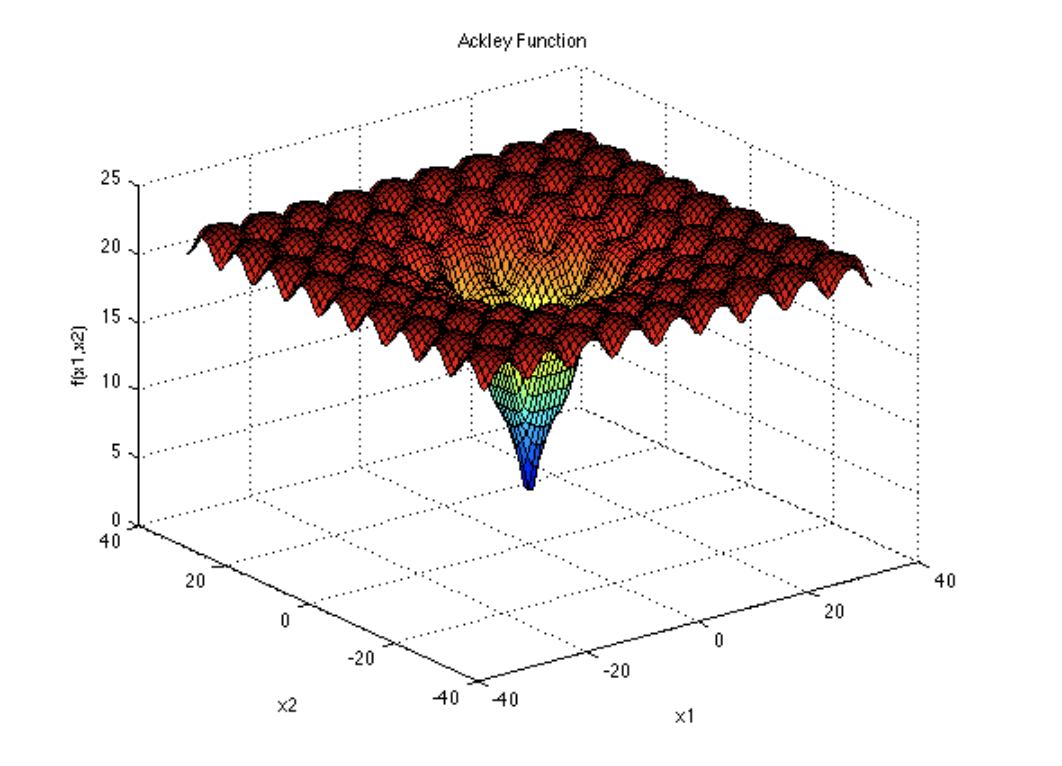
\includegraphics[width=0.8\linewidth]{ackley.png} 
    \caption{Two variable Ackley function. Figure reproduced from \cite{surjanovic_ackley_2013}.}
    \label{fig:ackley}
\end{figure}

I added an integration test to \gls{ROLLO} that checks that a default \gls{ROLLO} 
simulation will find the Ackley function's global minimum point. 
If \gls{ROLLO} performed sub-optimally, it would return one of the Ackley 
function's many local minimums. 

\subsection{Binh and Korn Function}
\label{sec:binhandkorn}
The Binh and Korn function \cite{binh_mobes_1997} is a two-objective function:
\begin{align}
    \mbox{Minimize} &= \begin{cases}
        f_1 (x_1,x_2) &= 4x_1^2+4x_2^2 \\
        f_2 (x_1,x_2) &= (x_1-5)^2 + (x_2-5)^2 
    \end{cases} \\
    \mbox{Such that} &= \begin{cases}
        (x_1-8)^2 + (x_2+3)^2 \geq 7.7 \nonumber \\
        0 \leq x_1 \leq 5, 0 \leq x_2 \leq 3 \nonumber
    \end{cases}
\end{align}
We use it as a performance test for multiobjective optimization.
% todo: why is this a good problem? what makes it a good evaluator. 
Figure \ref{fig:binh_paretofront} shows the Binh and Korn function's Pareto front.
\begin{figure}[htbp]
    \centering
    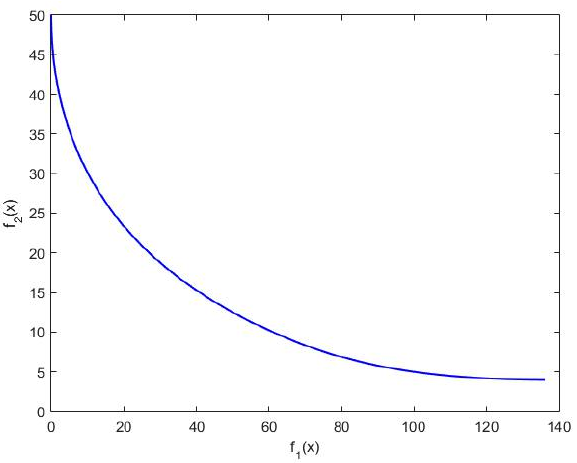
\includegraphics[width=0.7\linewidth]{binh-paretofront.png} 
    \caption{Pareto front of the Binh and Korn test function. Figure reproduced from 
    \cite{bassi_statistics_2018}. }
    \label{fig:binh_paretofront}
\end{figure}
I use the hypervolume indicator to quantify the Pareto front's quality. 
The hypervolume indicator is the most used set-quality indicator for assessing 
stochastic multiobjective optimizers \cite{guerreiro_hypervolume_2020}.
The hypervolume indicator measures the volume (in the objective space) covered by 
non-dominated solutions for problems in which all objectives are to be 
minimized \cite{deb_multi-objective_2001}. 
% todo: remind us of how the reference point is chosen and how it affects hypervolume. 
Figure \ref{fig:pareto_hypervolume} illustrates the hypervolume enclosed by the 
non-dominated solutions (A, B, C, D, E) and reference point, W, in the hatched region 
for a two-dimensional problem.
\begin{figure}[htbp]
    \centering
    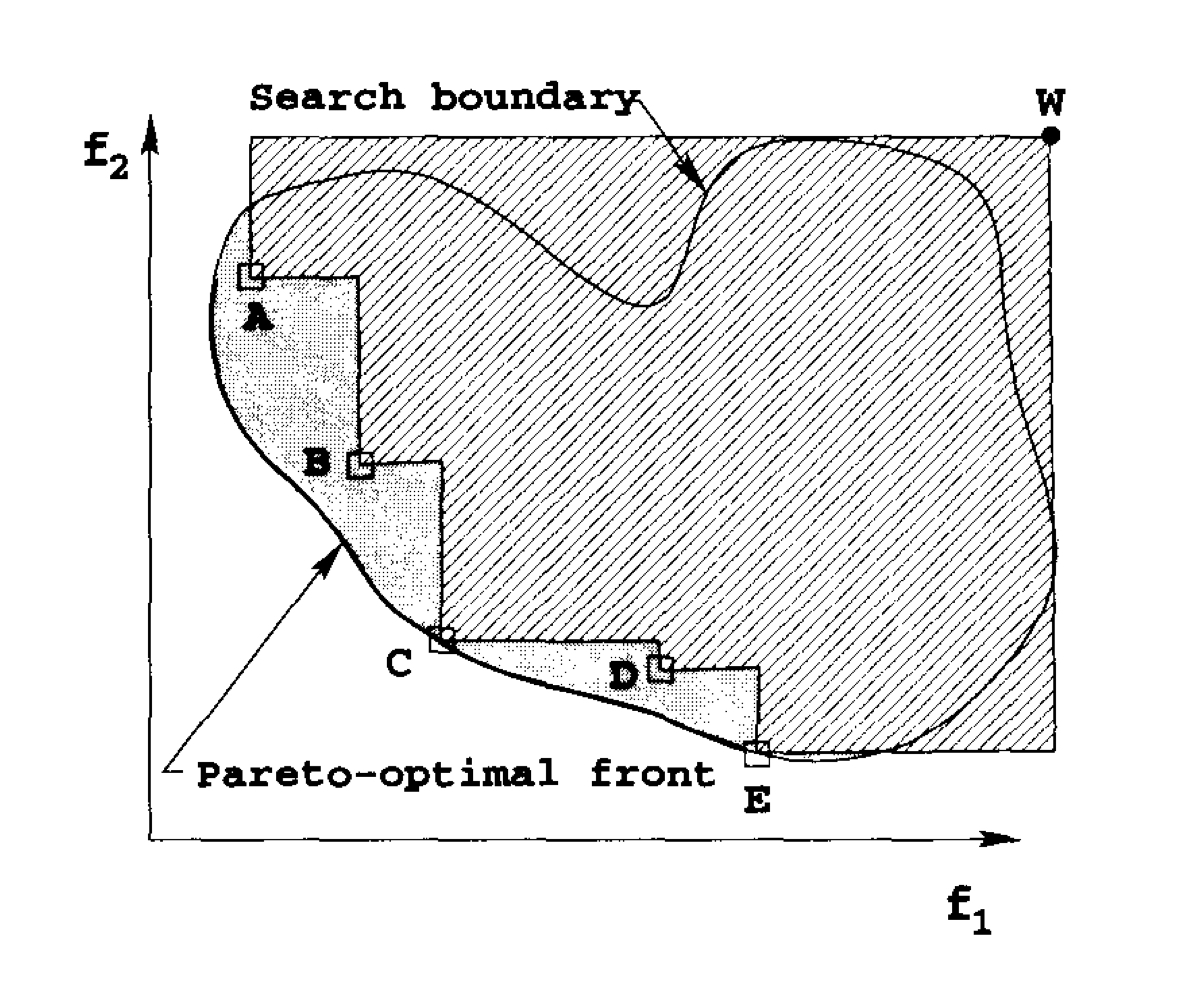
\includegraphics[width=0.7\linewidth]{pareto-hypervolume.png} 
    \caption{Example hypervolume enclosed by non-dominated solutions. Figure reproduced 
    from \cite{deb_multi-objective_2001}. 
    The f1 and f2 axes correspond to the optimization objectives in a \gls{ROLLO} 
    simulation. }
    \label{fig:pareto_hypervolume}
\end{figure}
I added an integration test to ROLLO that checks that a ROLLO simulation will 
find a hypervolume comparable to the ideal Pareto front when minimizing the
Binh and Korn function. 

\subsection{Pu-239 Critical Bare Sphere}
I ran a neutronics verification problem: finding the critical radius for a $^{239}Pu$ 
bare sphere, to ensure successful coupling between \gls{ROLLO} and reactor neutronics 
modeling software, OpenMC \cite{romano_openmc:_2015}. 
The solution to this problem is well studied and readily available in the 
literature \cite{blanchard_updated_1999}. 
Blanchard et al reported that with MCNP4b code and ENDF/B-VI data library, the 
critical mass of a Pu239 bare sphere is 10.00 kg which corresponds to a diameter 
of 9.9cm \cite{blanchard_updated_1999}.
Figure \ref{fig:verification-sphere} shows the ROLLO input file for this verification 
problem. 
In the input file, I vary the radius between 1.0 and 8.0cm, with the objective of 
minimizing the radius while constraining the problem to have $k_{eff} >= 1.0$.
\begin{figure}[htbp]
    \begin{minted}[
        frame=lines,
        framesep=2mm,
        baselinestretch=1.2,
        fontsize=\footnotesize,
        linenos
        ]{json}
        {"control_variables": {
                "radius": {"min": 1.0, "max": 8.0}
            },
            "evaluators": {
                "openmc": {
                    "order": 0,
                    "input_script": ["python", "critical_sphere.py"],
                    "inputs": ["radius"],
                    "outputs": ["keff", "radius"],
                    "output_script": ["python", "get_sphere_keff.py"]
                }
            },
            "constraints": {"keff": {"operator": [">="], 
                            "constrained_val": [1.0]}},
            "algorithm": {
                "parallel": "multiprocessing",
                "keep_files": "none",
                "objective": ["min"],
                "optimized_variable": ["radius"],
                "pop_size": 80,
                "generations": 10
            }}
    \end{minted}
    \caption{\acrfull{ROLLO} JSON input file for finding the minimum radius for 
    a $^{239}Pu$ Critical Bare Sphere.}
    \label{fig:verification-sphere}
\end{figure}
\pagebreak
Figure \ref{fig:critical_sphere.py} shows the OpenMC template used in the 
\gls{ROLLO} simulation. 
\begin{figure}[htbp]
    \begin{minted}[
        frame=lines,
        framesep=2mm,
        baselinestretch=1.2,
        fontsize=\footnotesize,
        linenos
        ]{python}
            import openmc 
            import numpy as np

            pu = openmc.Material()
            pu.set_density("g/cm3", 19.84)
            pu.add_nuclide("Pu239", 1)
            mats = openmc.Materials([pu])
            
            radius = {{radius}}
            
            fuel_sphere = openmc.Sphere(r=radius, boundary_type='vacuum')
            fuel_cell = openmc.Cell(fill=pu, region=-fuel_sphere)
            univ = openmc.Universe(cells=[fuel_cell])
            geom = openmc.Geometry(univ)
            
            settings = openmc.Settings()
            settings.batches = 100
            settings.inactive = 20
            settings.particles = 20000
            settings.temperature = {"multipole": True, "method": "interpolation"}
            
            mats.export_to_xml()
            geom.export_to_xml()
            settings.export_to_xml()
            openmc.run()
    \end{minted}
    \caption{OpenMC template input file used in ROLLO simulation to find the 
    minimum radius for a $^{239}Pu$ Critical Bare Sphere.}
    \label{fig:critical_sphere.py}
\end{figure}  

\gls{ROLLO} successfully finds the critical radius of the $^{239}Pu$ bare sphere 
to be 4.9856cm which corresponds to approximately a 9.9cm diameter. 
The critical sphere's $k_{eff}$ value is 1.00919 $\pm$ 0.00048. 
Figure \ref{fig:verification-radius} and \ref{fig:verification-keff} show the 
radius and $k_{eff}$ evolution through the evolutionary algorithm's 
generations. 
They demonstrate how the average radius converges towards the critical radius while 
constraining $k_{eff} \geq 1$ and improving with each generation.
\begin{figure}[htbp]
    \centering
    \begin{subfigure}{\textwidth}
    \makebox[\textwidth][c]{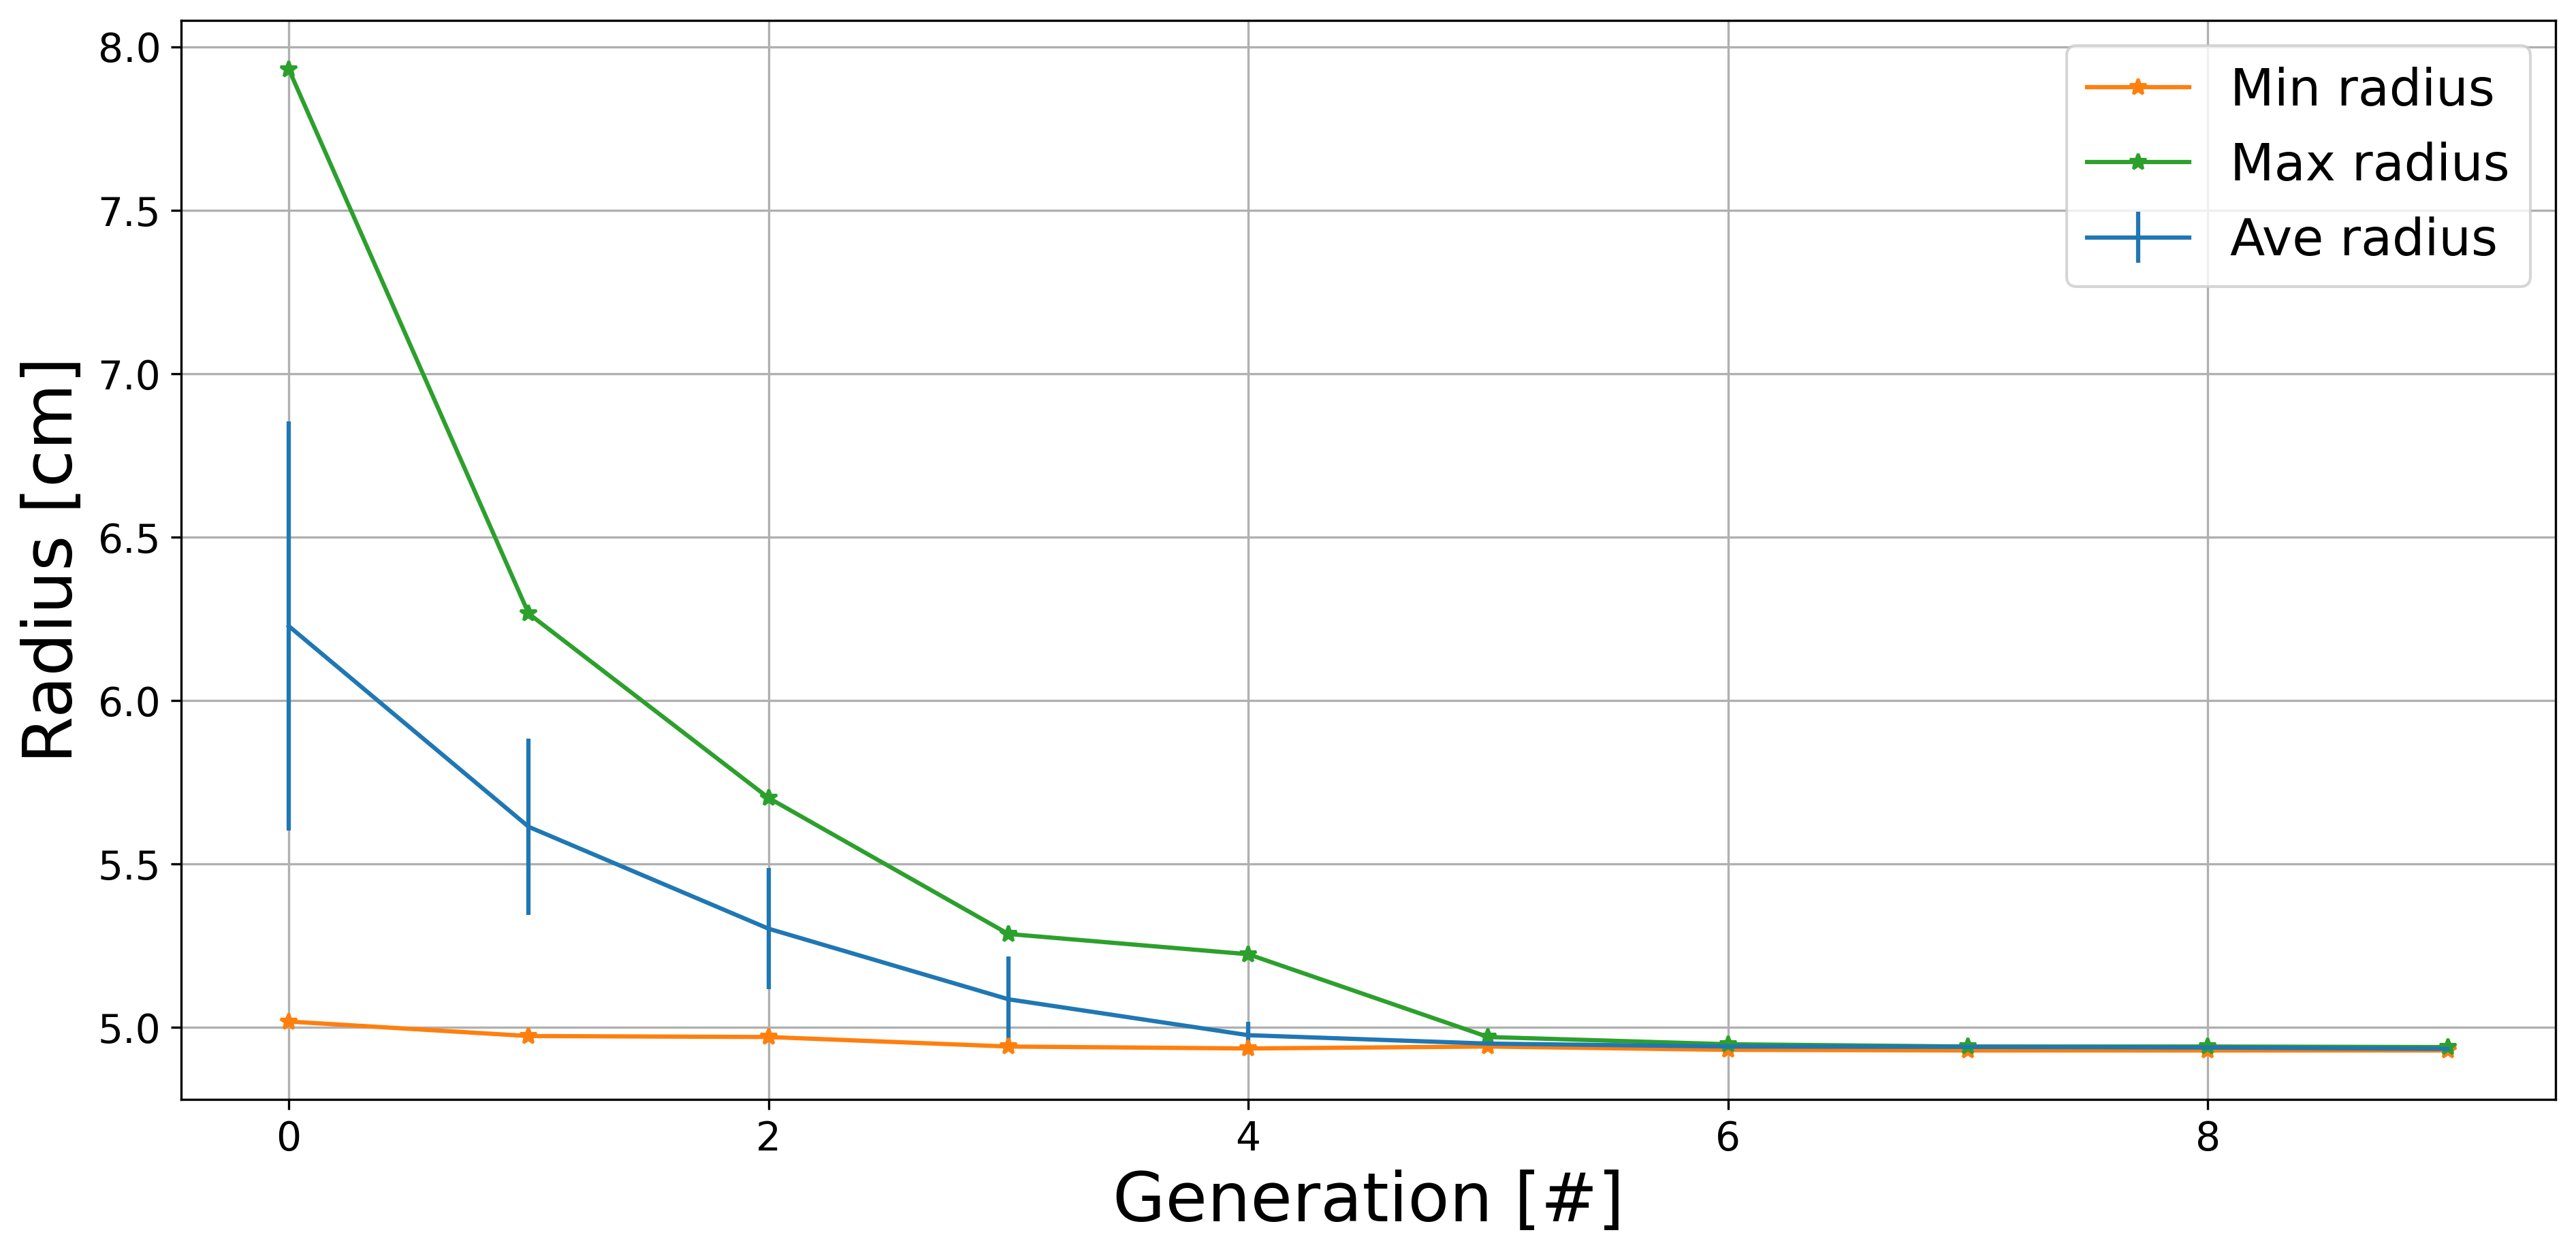
\includegraphics[width=1.1\linewidth]{radius-convergence.png}} 
    \caption{Minimum, average, and maximum radius values evolution.}
    \label{fig:verification-radius}
    \end{subfigure}
    \begin{subfigure}{\textwidth}
        \makebox[\textwidth][c]{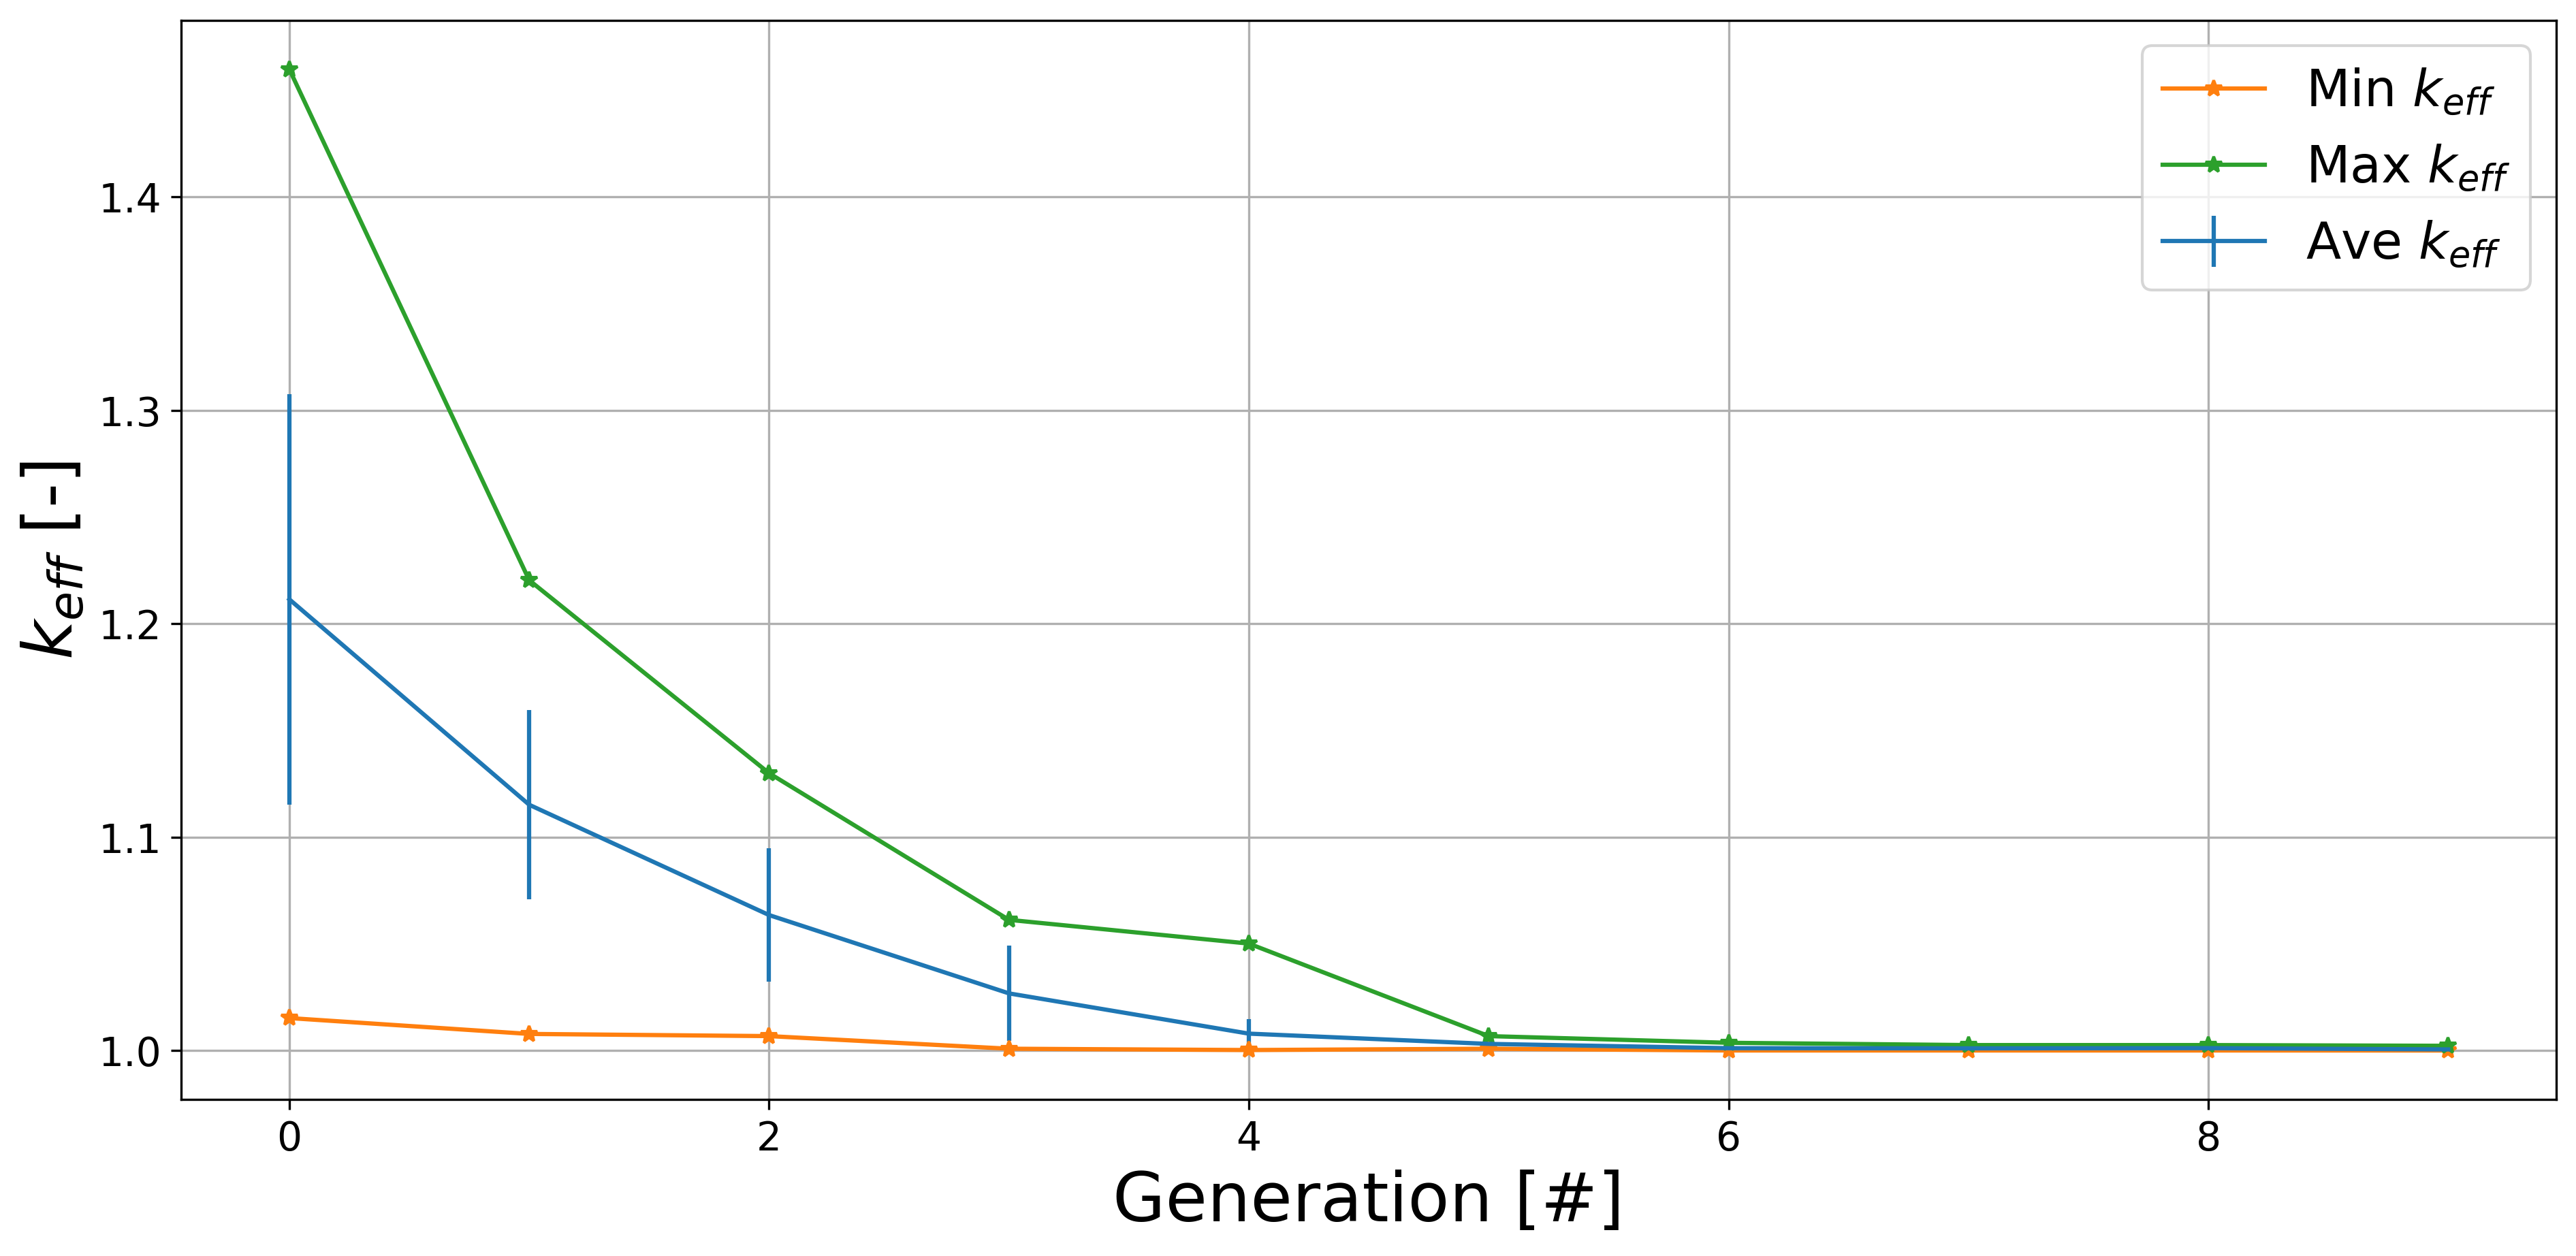
\includegraphics[width=1.1\linewidth]{keff-convergence.png}}
        \caption{Minimum, average, and maximum $k_{eff}$ values evolution.}
        \label{fig:verification-keff}
    \end{subfigure}
    \caption{Results for each generation for \gls{ROLLO}'s genetic algorithm optimization 
    to the find the critical radius of a  $^{239}Pu$ bare sphere.}
\end{figure}

\section{ROLLO Convergence Criteria}
The \texttt{generations} input parameter defines \gls{ROLLO}'s evolutionary algorithm 
convergence criterion. 
Each nuclear reactor model's evaluation is computationally intensive. 
Users will most likely be constrained by the total available compute time. 
Therefore, rather than setting a results-based stopping criterion, ROLLO enables 
users to define the \texttt{generations} and \texttt{pop$\_$size} based on the 
amount of compute time available to them: 
\begin{align}
    t_{total} &= t_{eval} \times gen \times pop 
\intertext{where}
    t_{total} &= \mbox{Total compute time available} \nonumber \\
    t_{eval} &= \mbox{compute time per nuclear reactor model evaluation} \nonumber \\
    gen &= \mbox{total number of generations in optimization process} \nonumber \\
    pop &= \mbox{population size in optimization process} \nonumber
\end{align} 

\subsection{Convergence}
\label{sec:rollo-convergence}
ROLLO does not utilize a mathematical expression to evaluate problem convergence. 
The complexity of reactor design optimization means that no single indicator determines 
if convergence is met.
Instead, ROLLO's purpose is to help the human reactor designer narrow down the design 
space. 
When a ROLLO run completes, the user plots the objectives' convergence and 
Pareto front (for multiobjective simulations) to evaluate if they are confident 
about the final solution set. 
Section \ref{sec:opt} described that an ideal optimization method for a 
multi-objective problem like reactor design should find widely spread solutions 
on the obtained Pareto front \cite{deb_multi-objective_2001}. 
If the simulation is not converged, the user can easily restart the optimization 
simulation using the \texttt{checkpoint.pkl} file and run the problem for a few more 
generations. 
% add about hypervolume for multiobj and obj convergence for singleobj

\section{Summary}
This chapter described the \acrfull{ROLLO} framework developed for 
this dissertation. 
\gls{ROLLO} is a Python package that applies evolutionary algorithm 
optimization techniques to nuclear reactor design using the \acrfull{DEAP} 
module. 
The motivation for \gls{ROLLO} is to enable reactor designers to utilize 
robust evolutionary algorithm optimization methods without going 
through the cumbersome process of setting up a genetic algorithm framework,
selecting appropriate hyperparameters, and setting up its parallelization. 
I designed \gls{ROLLO} to be effective, flexible, open-source, parallel, 
reproducible, and usable. 
\gls{ROLLO} is hosted on Github \cite{chee_rollo_2021}. 

\section{AHTR Optimization for Non-Conventional Designs}
\subsection{Optimization Methodology}
\begin{frame}
    \frametitle{AHTR Optimization Problem Definitions}
    \vspace{-0.2cm}
    \visible<1->{\begin{block}{Varied Input Parameters}
        \begin{itemize}
            \item Total fuel packing fraction ($PF_{total}$)
            \item TRISO fuel packing fraction distribution ($\rho_{TRISO}(\vec{r})$)
            \item Coolant channel shape ($r_i$)
        \end{itemize}}
        \visible<2->{Varying $PF_{total}$ and $\rho_{TRISO}(\vec{r})$ synergistically 
        explores how \textbf{heterogenous TRISO distribution could minimize 
        self-shielding} and thus, reduce the fuel required.}
    \end{block}
    \vspace{-0.3cm}
    \visible<3->{\begin{block}{AHTR Optimization Objectives}
     \textbf{Minimize total fuel packing fraction ($PF_{total}$)}
     \begin{itemize}
        \item Cost savings, non-proliferation 
     \end{itemize}
     \textbf{Minimize maximum temperature ($T_{max}$)}
     \begin{itemize}
        \item Minimize thermal stress in the fuel 
     \end{itemize}
     \textbf{Minimize fuel-normalized power peaking factor ($PPF_{fuel}$)} 
     \begin{itemize}
        \item Efficient fuel utilization
     \end{itemize}
    \end{block}}
    \visible<4->{\textbf{I optimized the AHTR plank and one-third assembly geometries.}} 
\end{frame}

\begin{frame}
    \frametitle{AHTR One-Third Assembly Geometry}
    \begin{figure}
        \only<1>{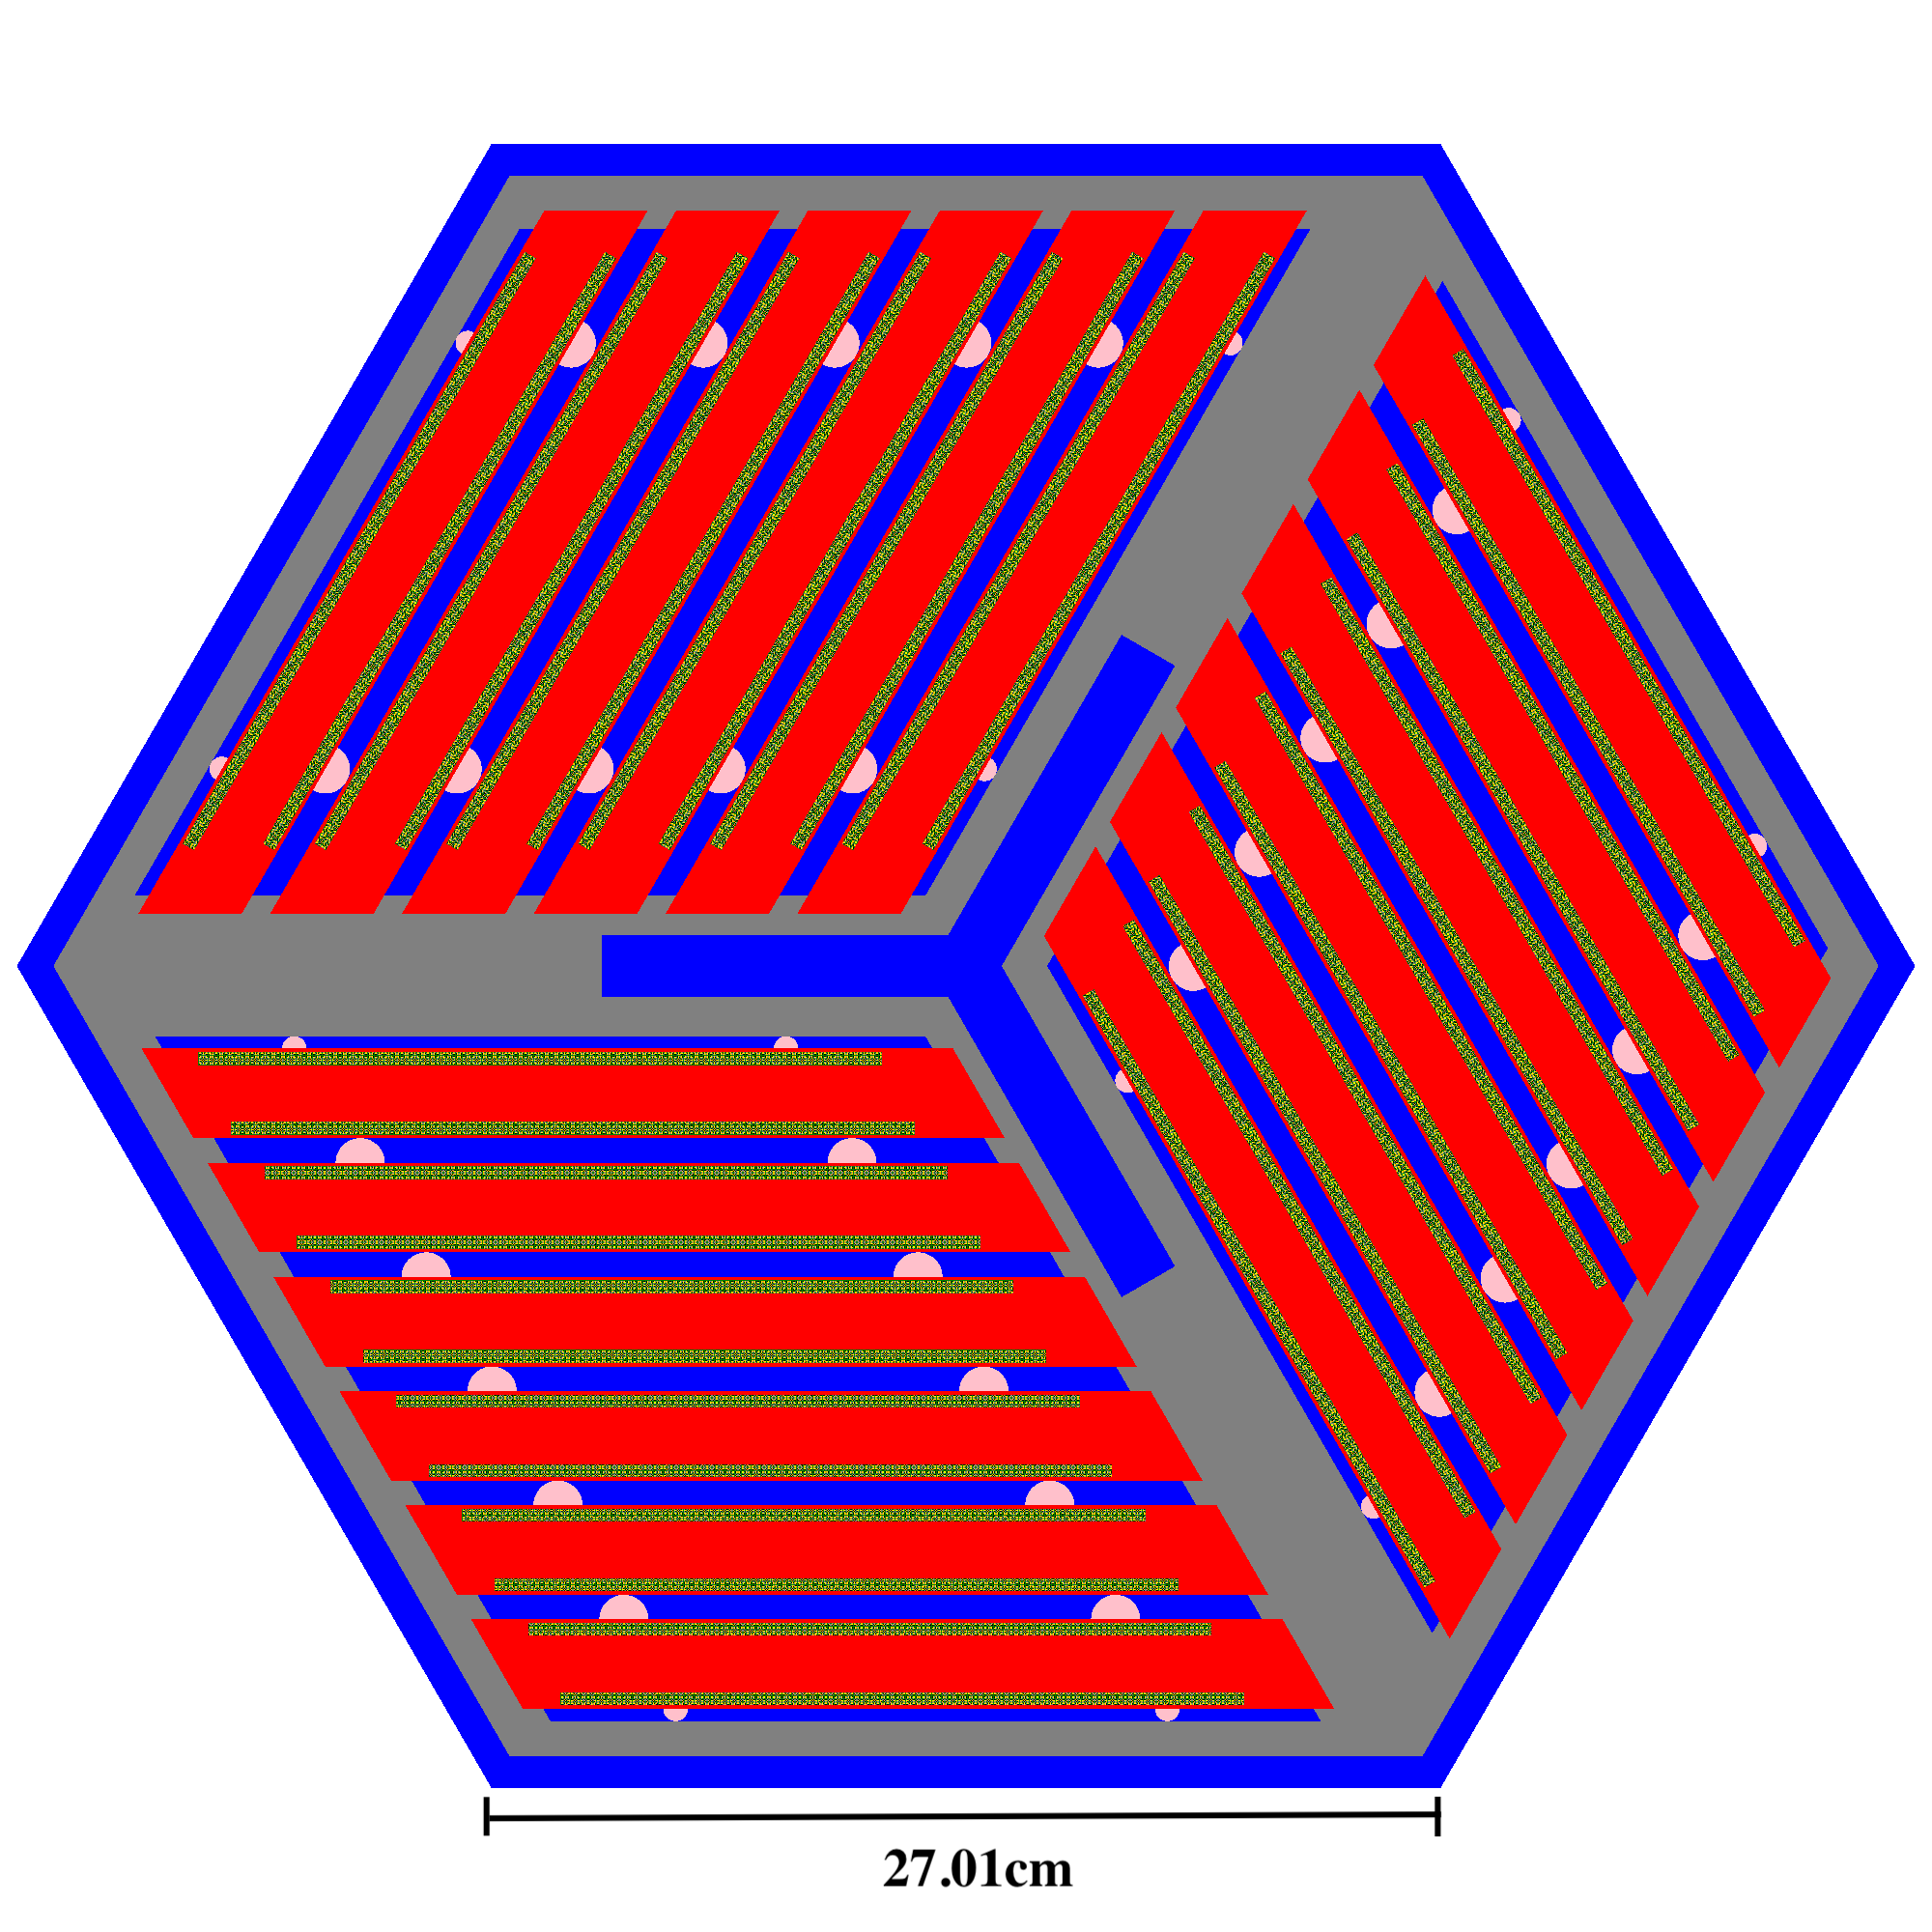
\includegraphics[width=0.6\linewidth]{../docs/figures/ahtr-fuel-element.png}} 
        \only<2>{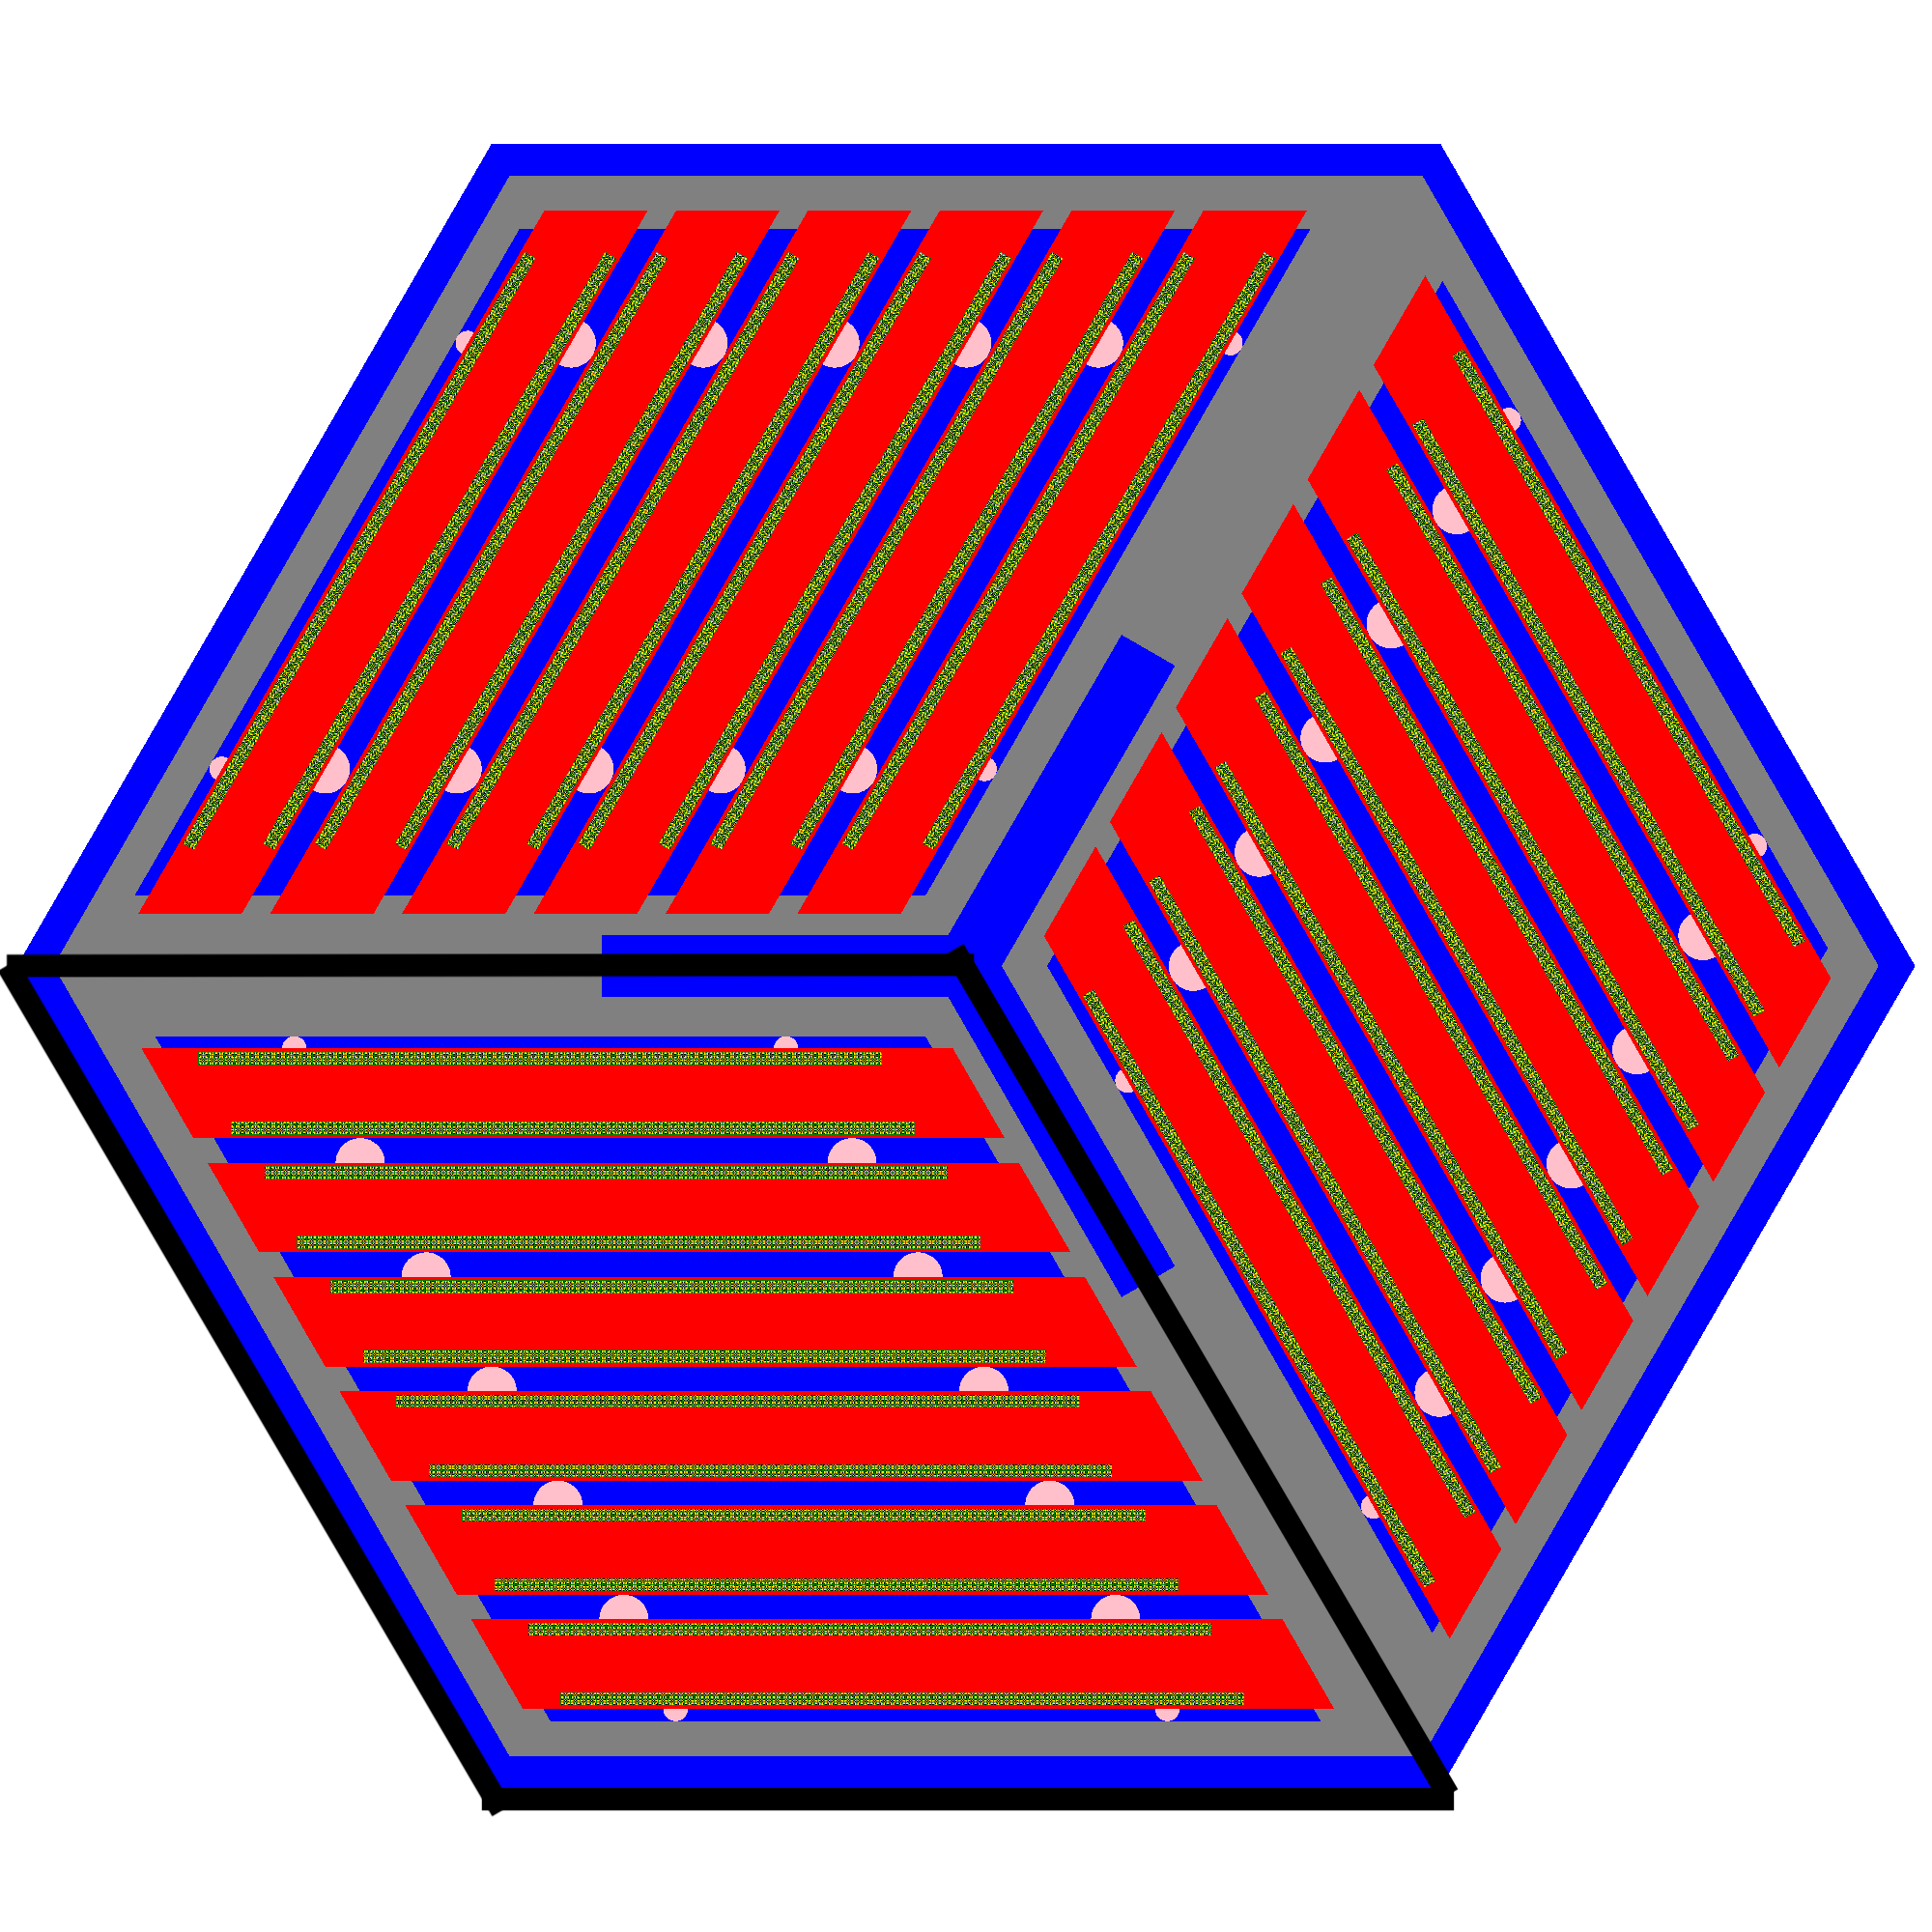
\includegraphics[width=0.6\linewidth]{figures/ahtr-fuel-element-annotated.png}} 
    \end{figure}
\end{frame}

\begin{frame}
    \frametitle{AHTR One-Third Assembly Geometry}
    \visible<1->{\textbf{Two sine distributions govern TRISO packing fraction distribution:}
    \begin{align}
    \rho_{TRISO}(\vec{x}, \vec{y}) &= \left(\textbf{a}\cdot sin(\textbf{b}\cdot 
    x + \textbf{c}) + 2\right) \cdot \left(\textbf{d}\cdot sin(\textbf{e}\cdot y + 
    \textbf{f}) + 2\right) \cdot NF \nonumber
    \end{align}
    
    The normalization factor (NF) ensures that total amount of TRISO particles in the 
    one-third assembly corresponds to $PF_{total}$.}

    \vspace{-0.3cm}
    \begin{columns}[t]
        \begin{column}{0.5\textwidth}
        \begin{figure}
            \only<1-2>{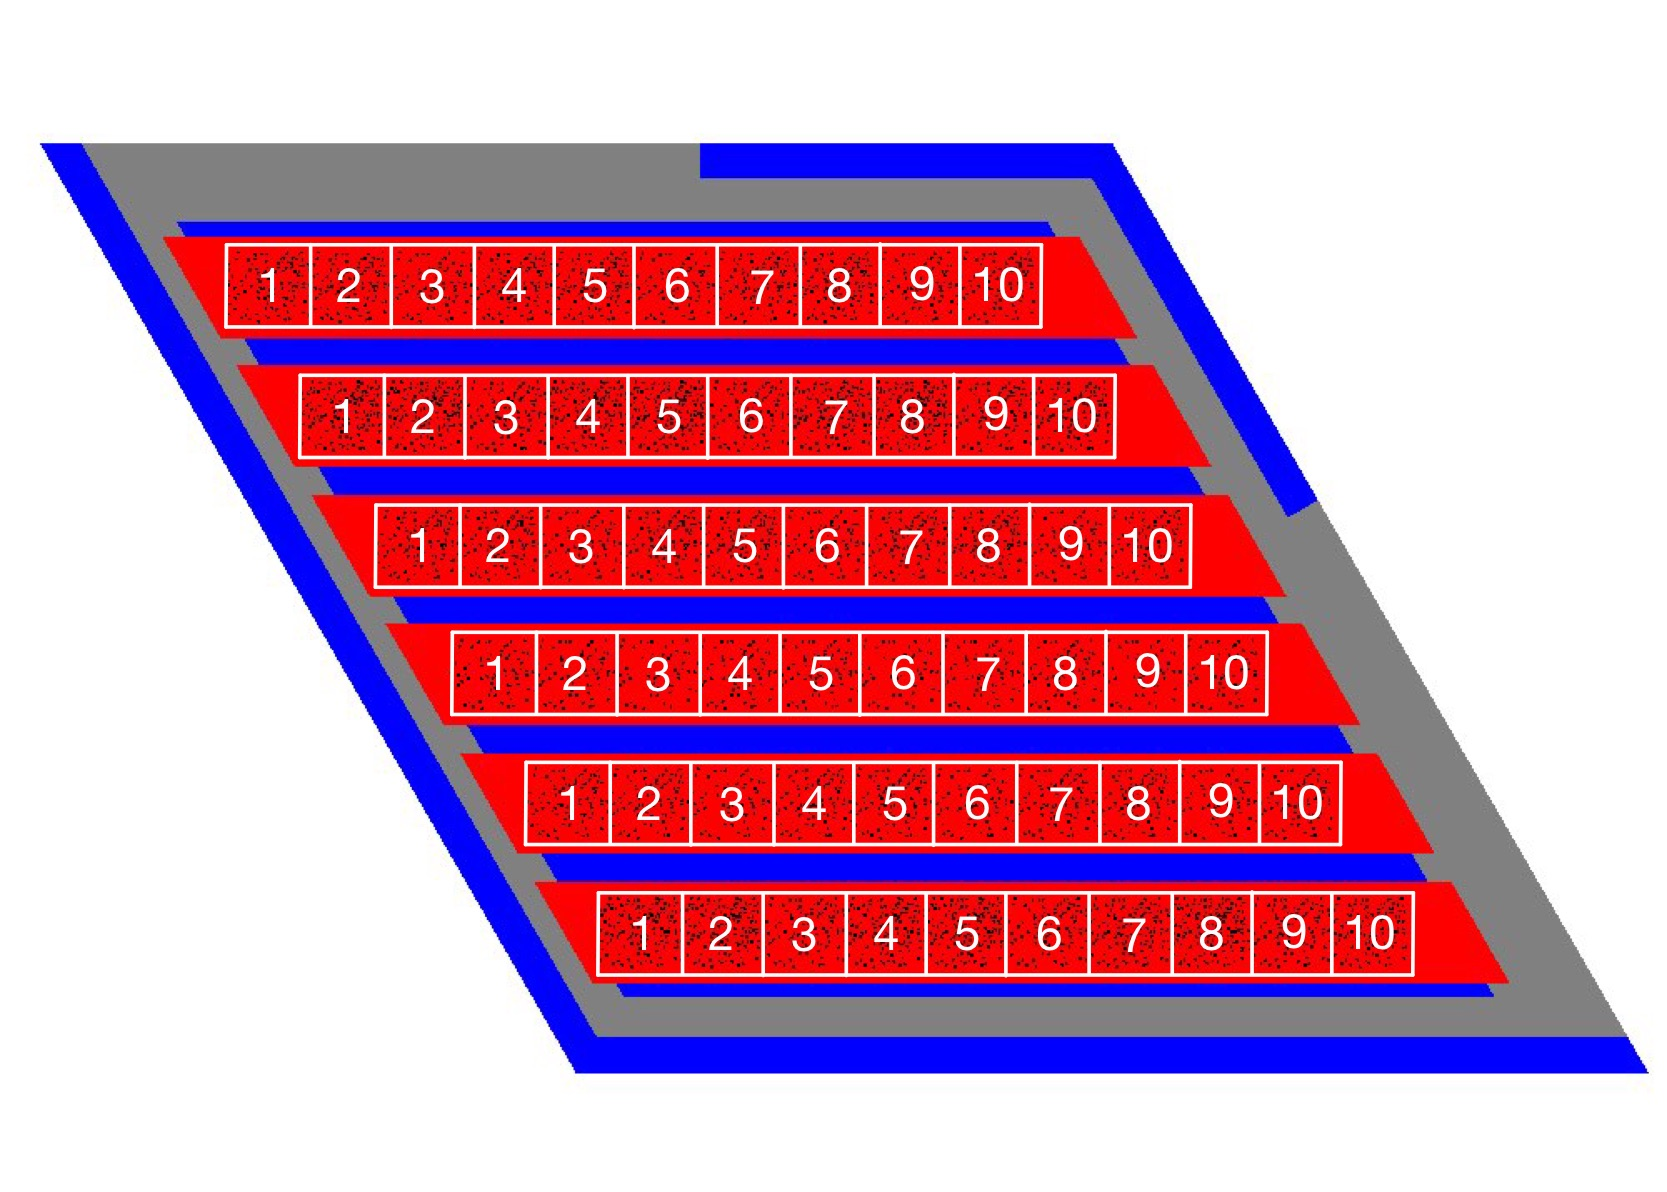
\includegraphics[width=\linewidth]{../docs/figures/ahtr_assembly.png} 
            \vspace{-0.6cm}
            \caption{AHTR one-third assembly illustrating packing fraction discretization.}}
            \only<3>{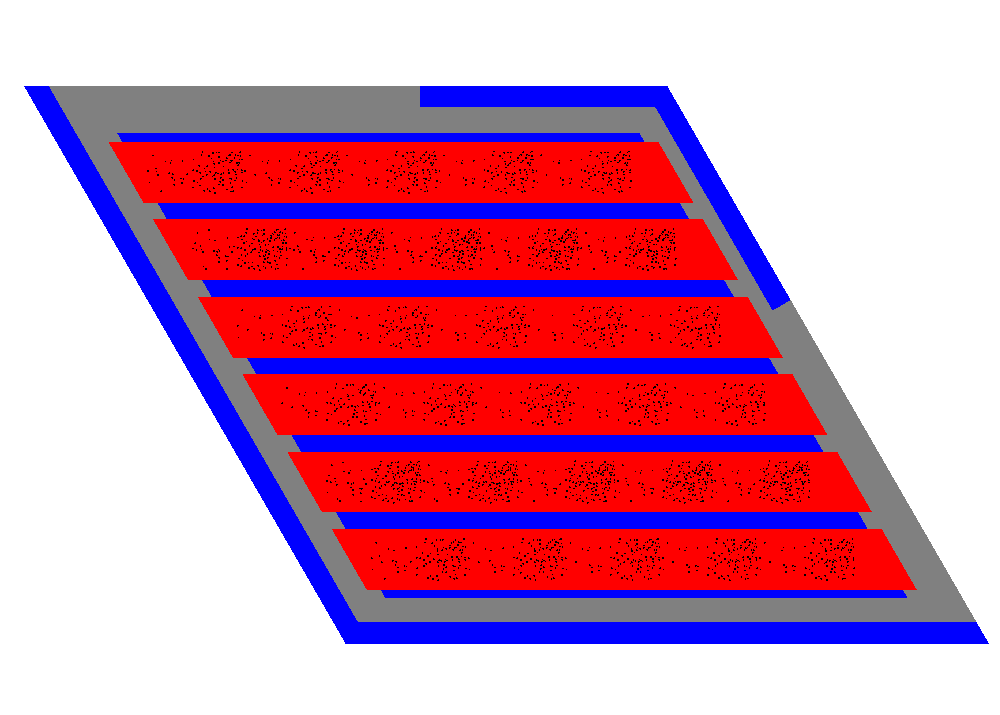
\includegraphics[width=\linewidth]{../docs/figures/assem-obj-1-pf-most-minimized.png} 
            \vspace{-0.6cm}
            \caption{AHTR one-third assembly illustrating packing fraction variation.}}
        \end{figure}
        \end{column}
        \begin{column}{0.5\textwidth} 
            \visible<2->{\begin{figure}
                \textbf{a} = 1.435, \textbf{b} = 1.488, \textbf{c} = 2.362, \\
                \textbf{d} = 0.689, \textbf{e} = 0.584, \textbf{f} = 4.170
                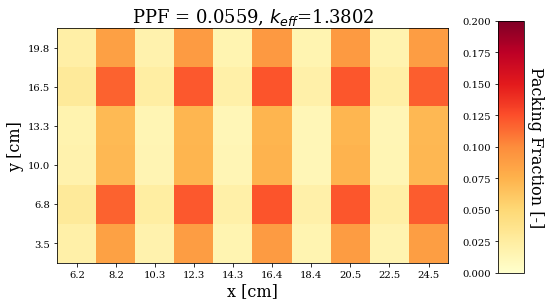
\includegraphics[width=\linewidth]{../docs/figures/assem-0.0559-most-minimized.png} 
                \caption{TRISO distribution example.}
            \end{figure}}
        \end{column}
        \end{columns}
\end{frame}

\begin{frame}
    \frametitle{Contd. AHTR One-Third Assembly Geometry}
    \textbf{Five radius values (\textbf{$r_1, r_2, r_3, r_4, r_5$}) 
    control coolant channel shape.}
    \begin{figure}
        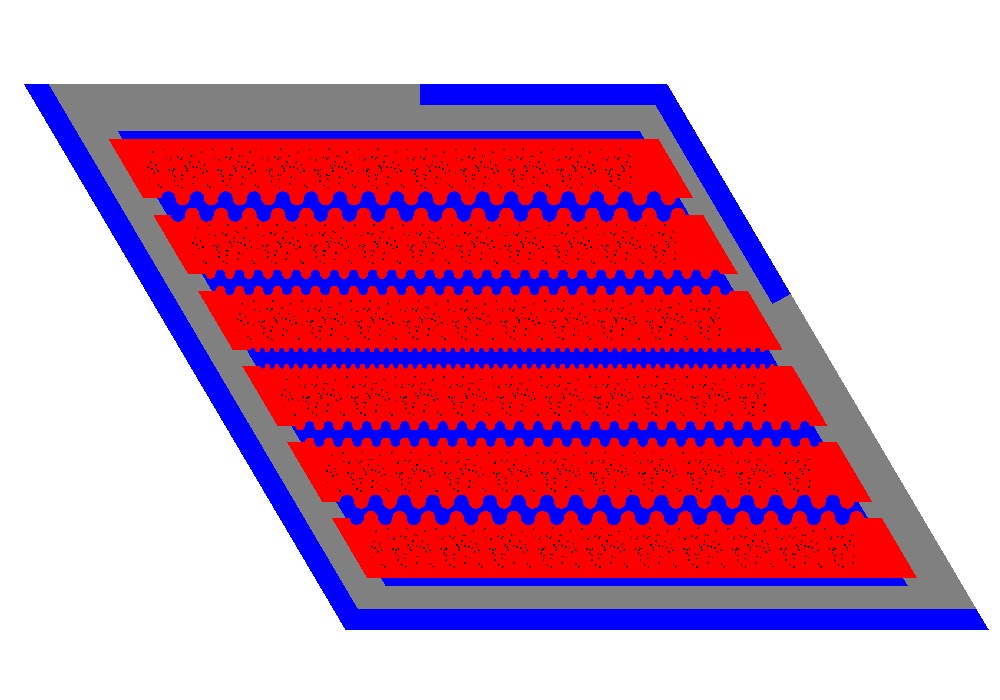
\includegraphics[width=0.7\linewidth]{../docs/figures/coolant-channel-shape-assem.png} 
        \vspace{-0.3cm}
        \caption{AHTR one-third assembly with coolant channel shape variation, 
        $r_1, r_2, r_3, r_4, r_5$ = 0.3cm, 0.2cm, 0.1cm, 0.2cm, 0.3cm.}
    \end{figure}
\end{frame}

\begin{frame}
    \frametitle{ROLLO AHTR Optimization Workflow}
    \vspace{-0.2cm}
    \begin{figure}
        \makebox[\textwidth][c]{
            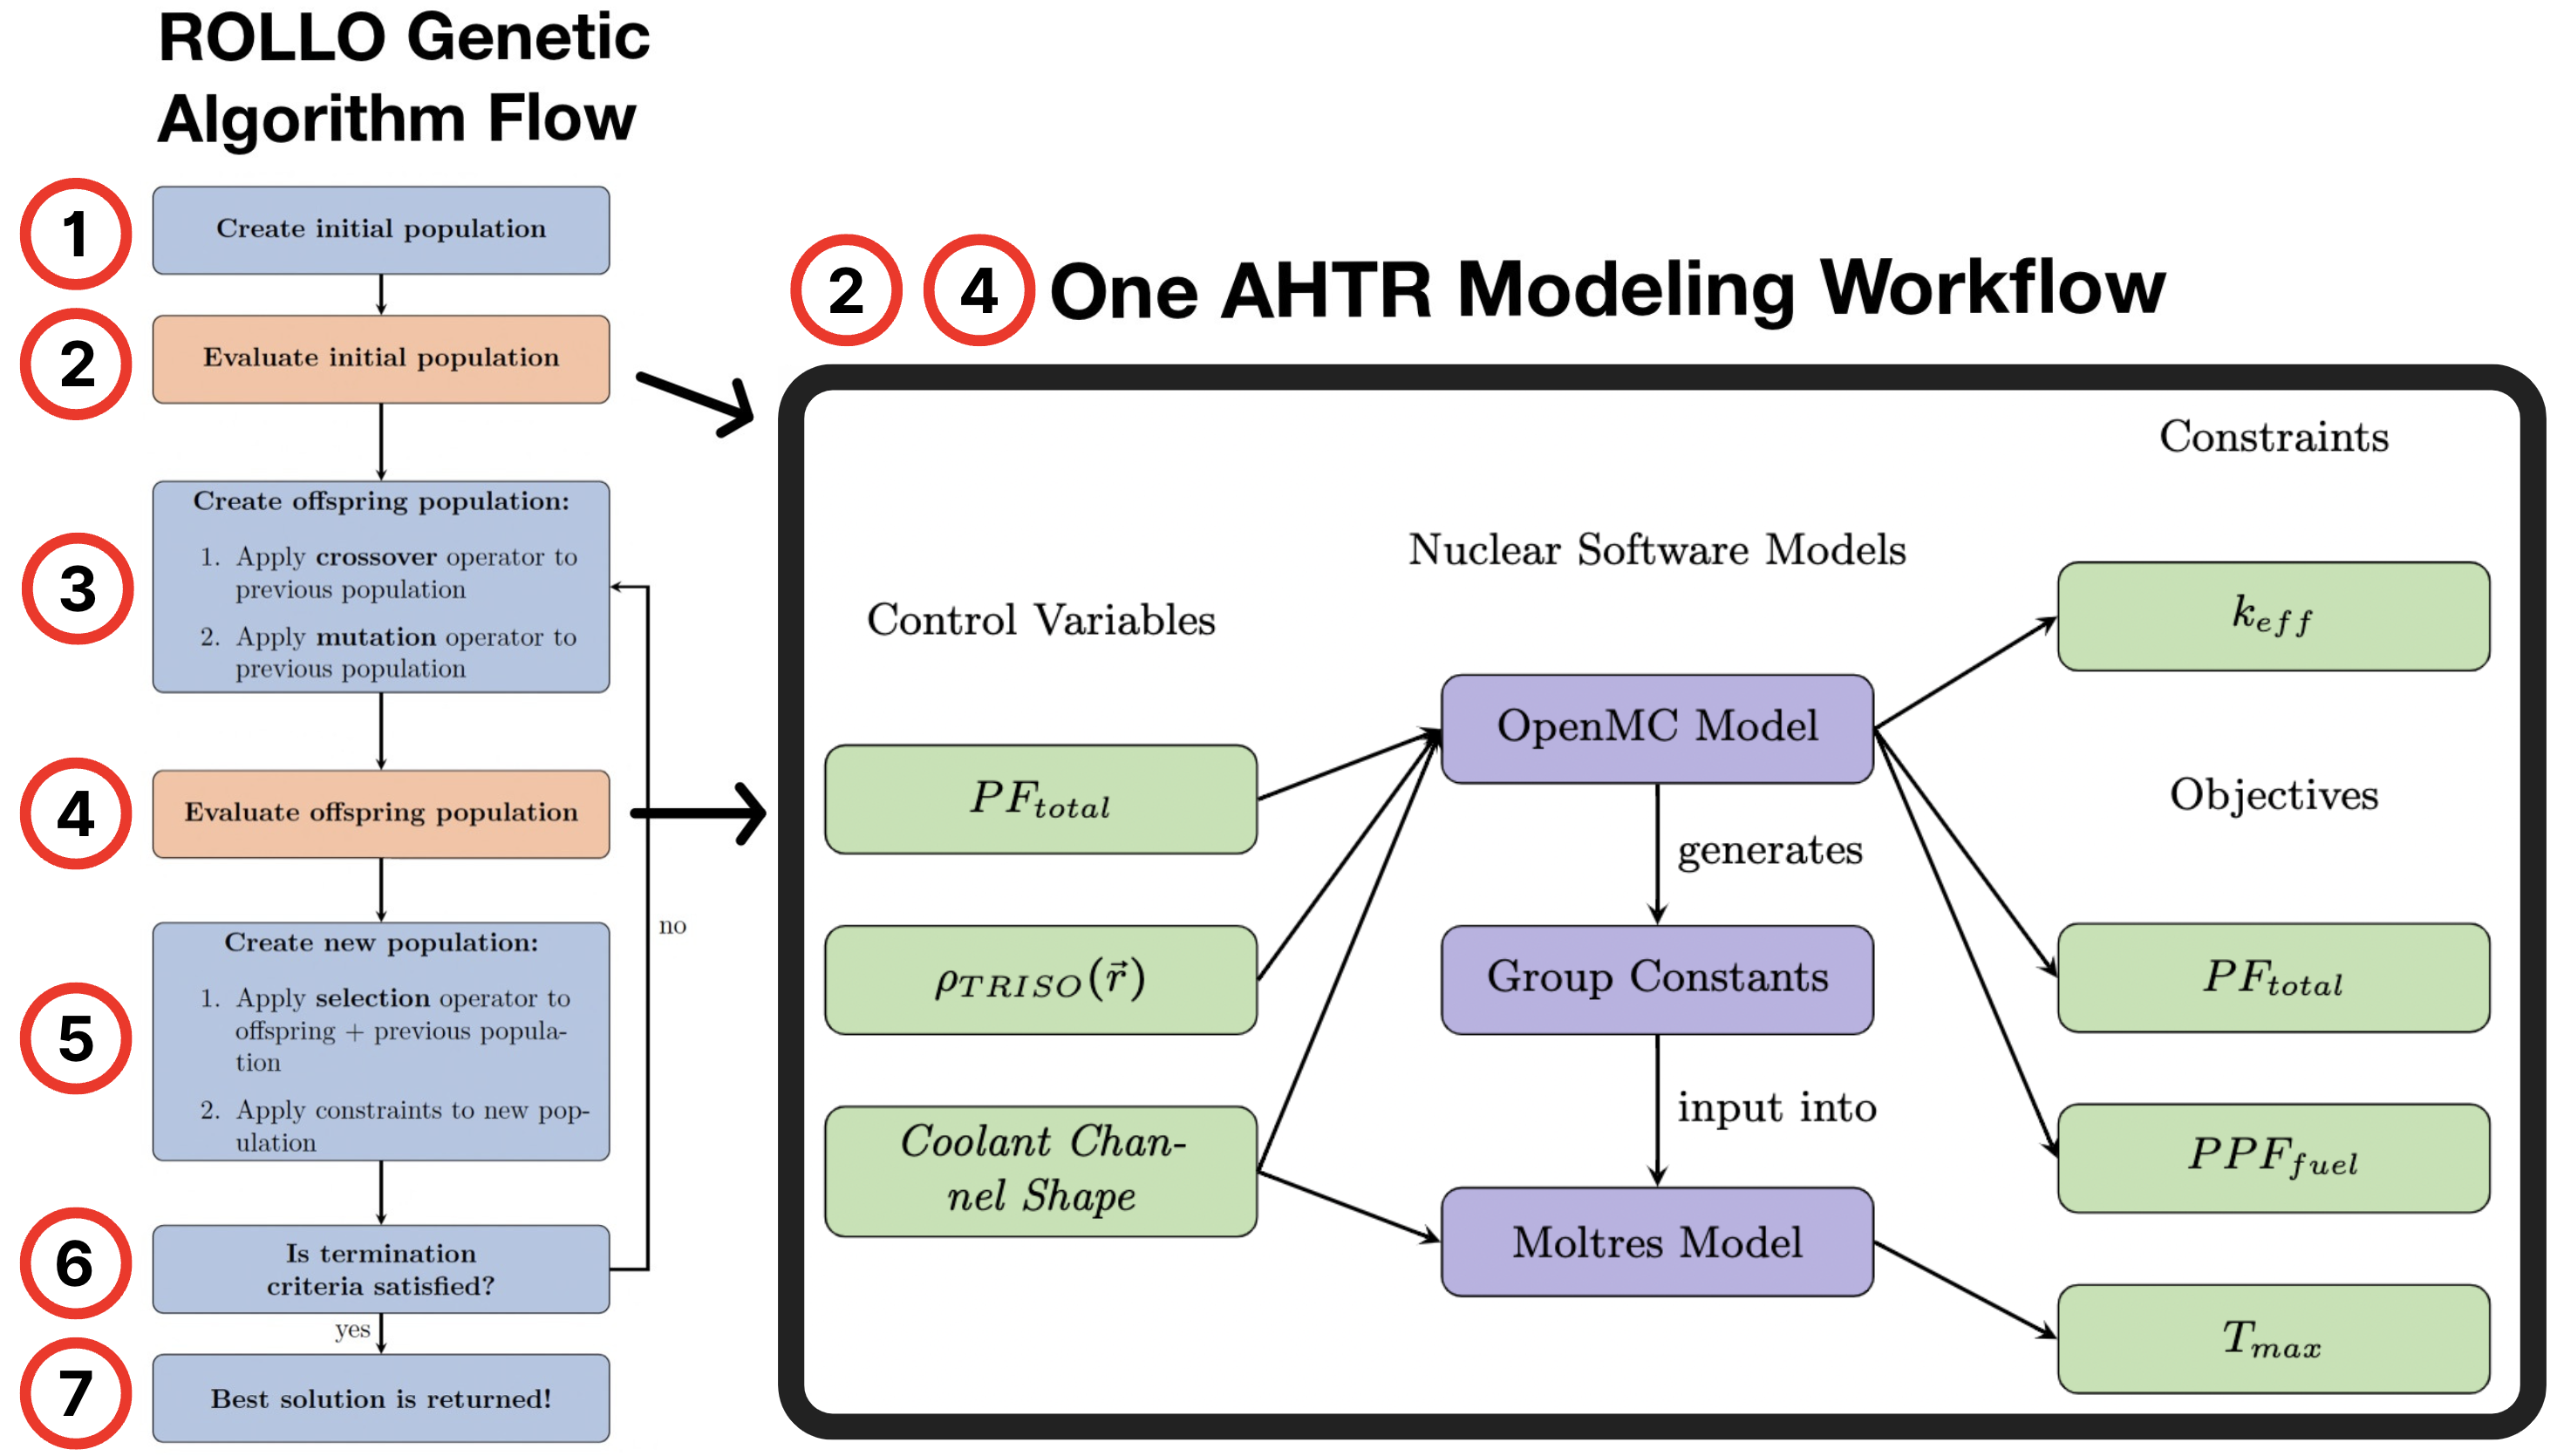
\includegraphics[width=1.1\linewidth]{figures/ahtr-modeling-workflow-numbered.png}} 
        %\caption{ROLLO AHTR Optimization Workflow.}
    \end{figure}
\end{frame}

\subsection{AHTR One-Third Assembly Optimization Results}
\begin{frame}
    \frametitle{AHTR One-Third Assembly Optimization Simulations}
    \only<1>{
        \vspace{-0.2cm}
        \begin{figure}
            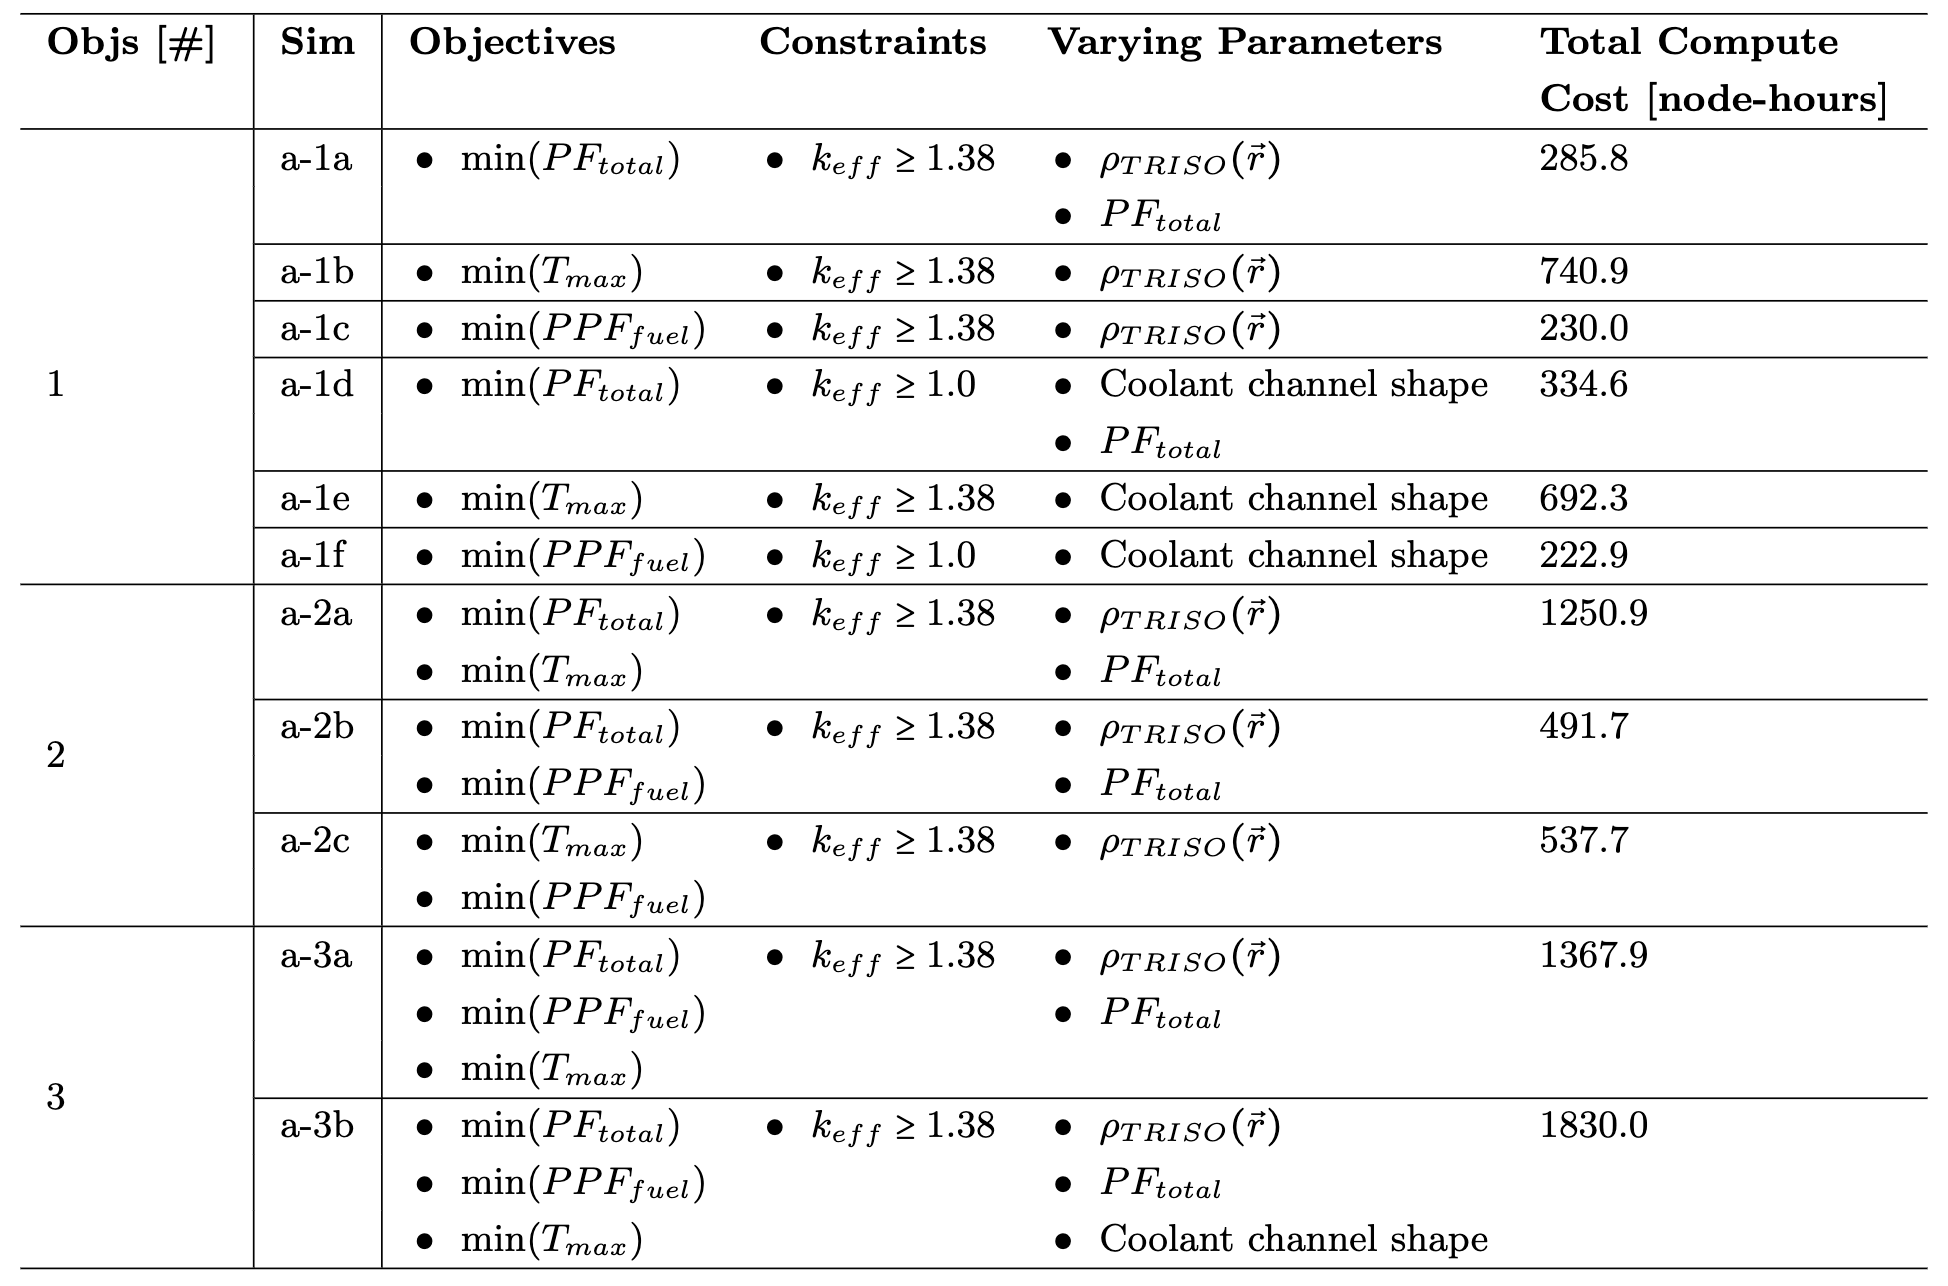
\includegraphics[width=0.8\linewidth]{figures/ahtr-assem-opt-table.png}
        \end{figure}

        \vspace{-0.2cm}
        \textbf{All the optimization simulations are run on the Theta supercomputer} 
        at the Argonne Leadership Computing Facility \cite{noauthor_thetathetagpu_2022}.

        Each Theta node has 64 1.3-GHz Intel Xeon Phi 7230 processors.
        }

        \only<2>{
            \begin{figure}
                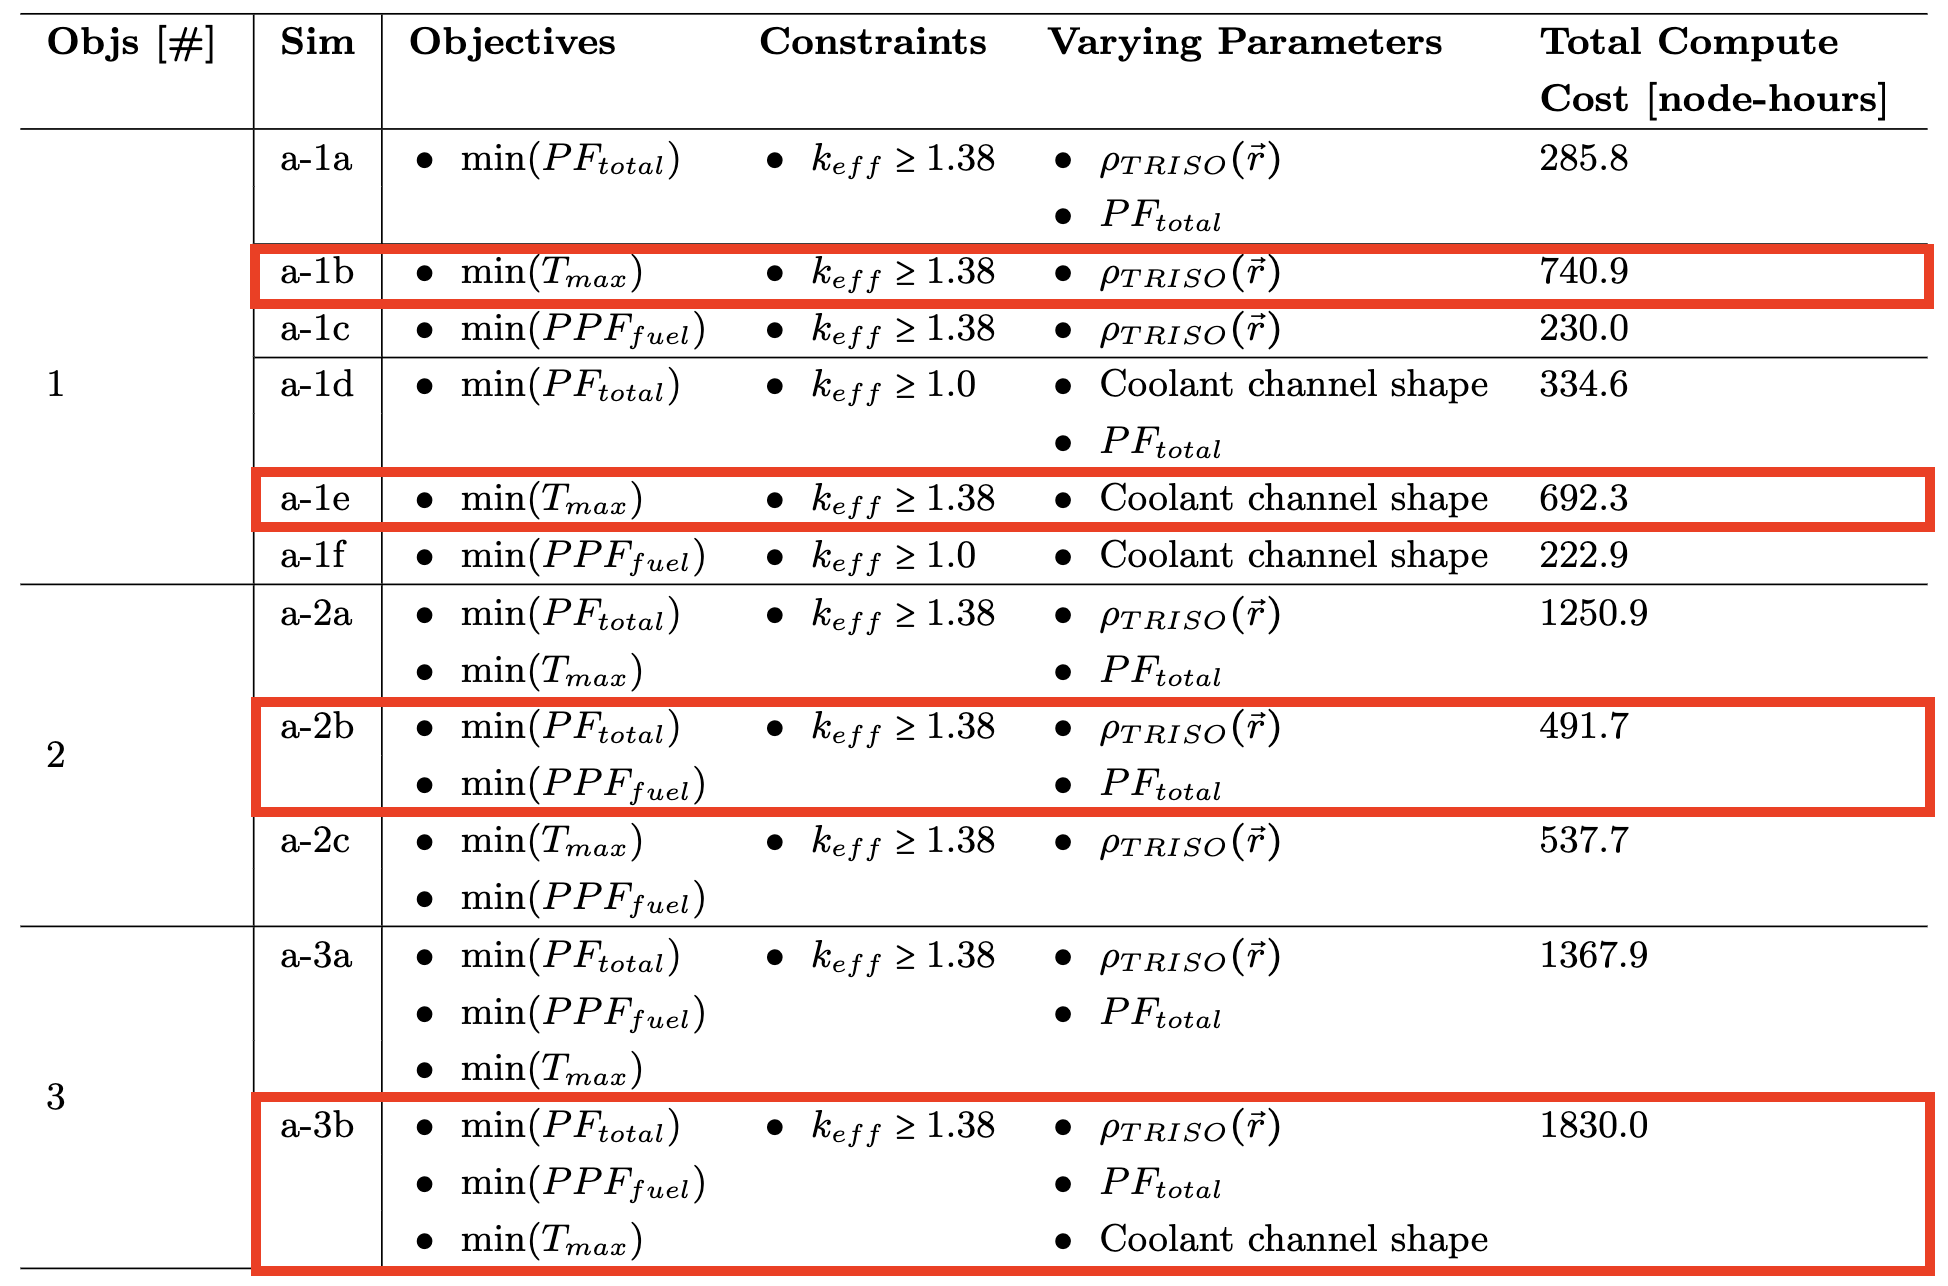
\includegraphics[width=0.9\linewidth]{figures/ahtr-assem-opt-table-annotated.png}
            \end{figure}}

        \only<3>{
            \begin{figure}
                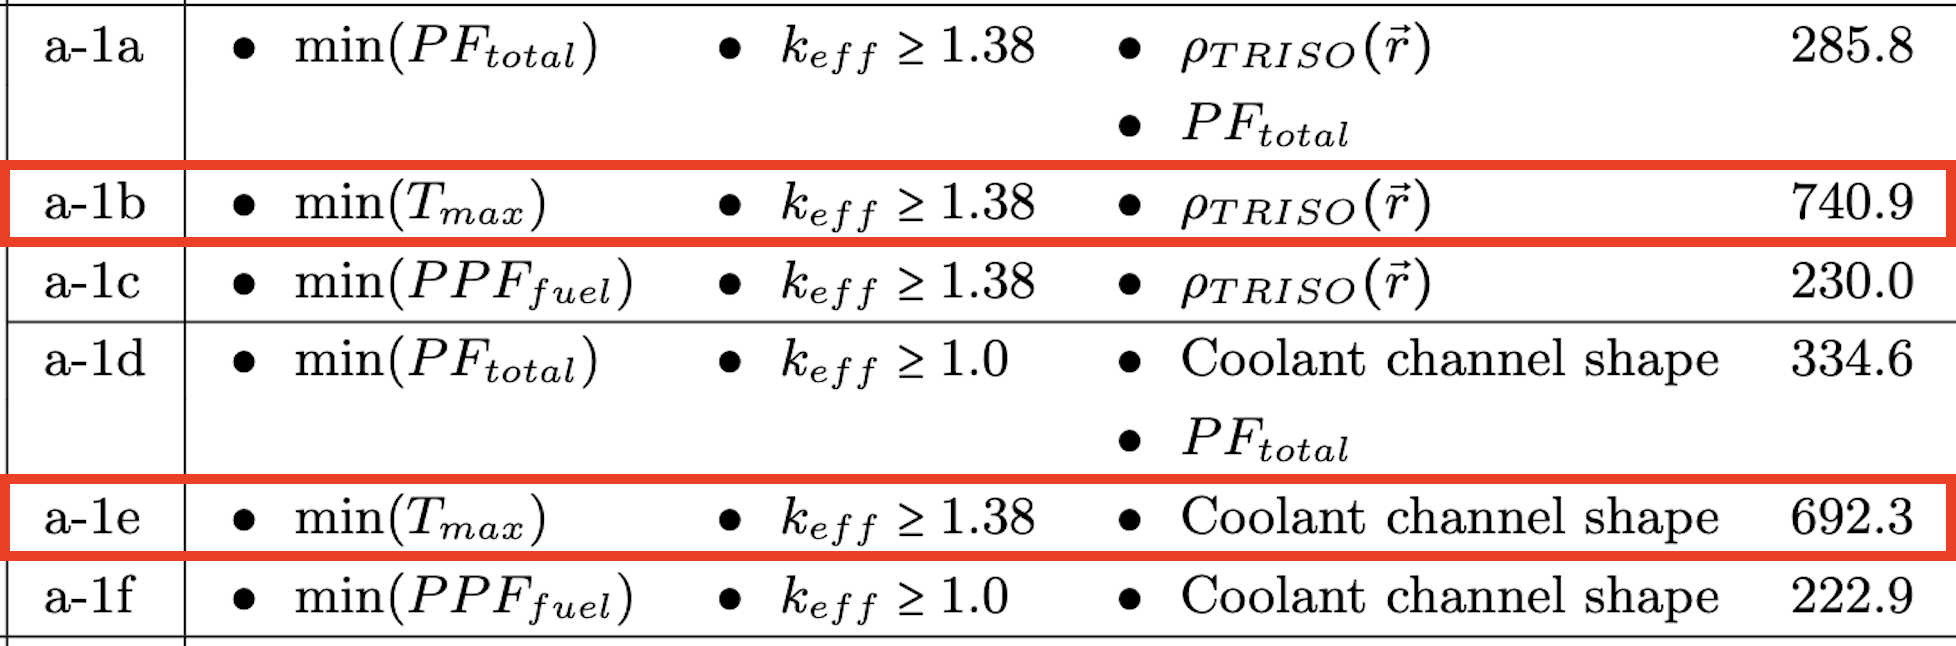
\includegraphics[width=\linewidth]{figures/ahtr-assem-opt-table-annotated1.png}
            \end{figure}
    
            Simulations a-1b and a-1e demonstrate \textbf{how the input parameters 
            $\rho_{TRISO}(\vec{r})$ and coolant channel shape respond to 
            the minimize $T_{max}$ objective}.

            \vspace{0.2cm}
            I constrained $k_{eff} \geq 1.38$ find optimal input parameters 
            that achieve \textbf{similar performance to the FHR benchmark} TRISO distribution.}
        
        \only<4>{
            \begin{figure}
                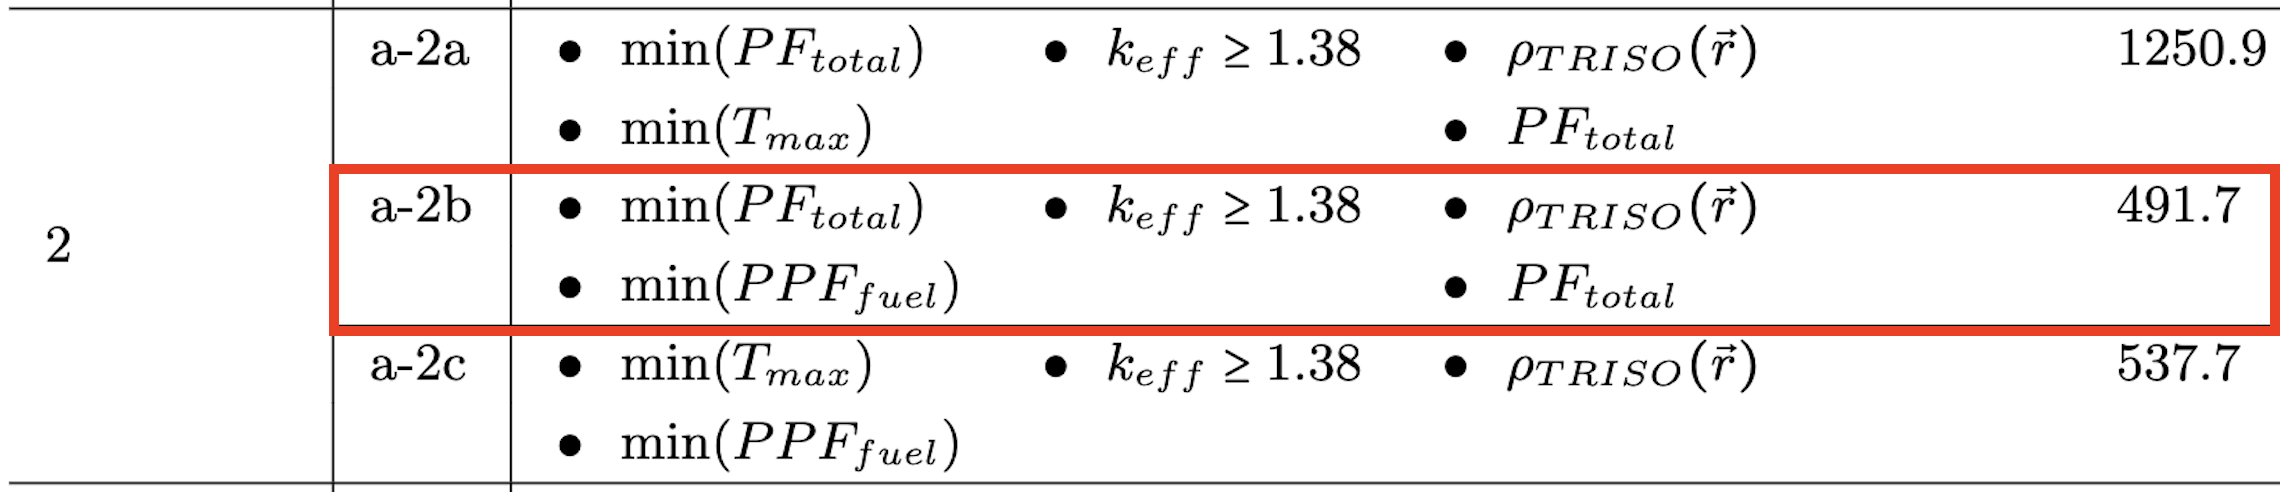
\includegraphics[width=\linewidth]{figures/ahtr-assem-opt-table-annotated2.png}
            \end{figure}

            Simulation a-2b demonstrates \textbf{how the input parameters $PF_{total}$ 
            and $\rho_{TRISO}(\vec{r})$ change as the minimize $PF_{total}$ and 
            $PPF_{fuel}$ objectives interact}.
        }

        \only<5>{
            \begin{figure}
                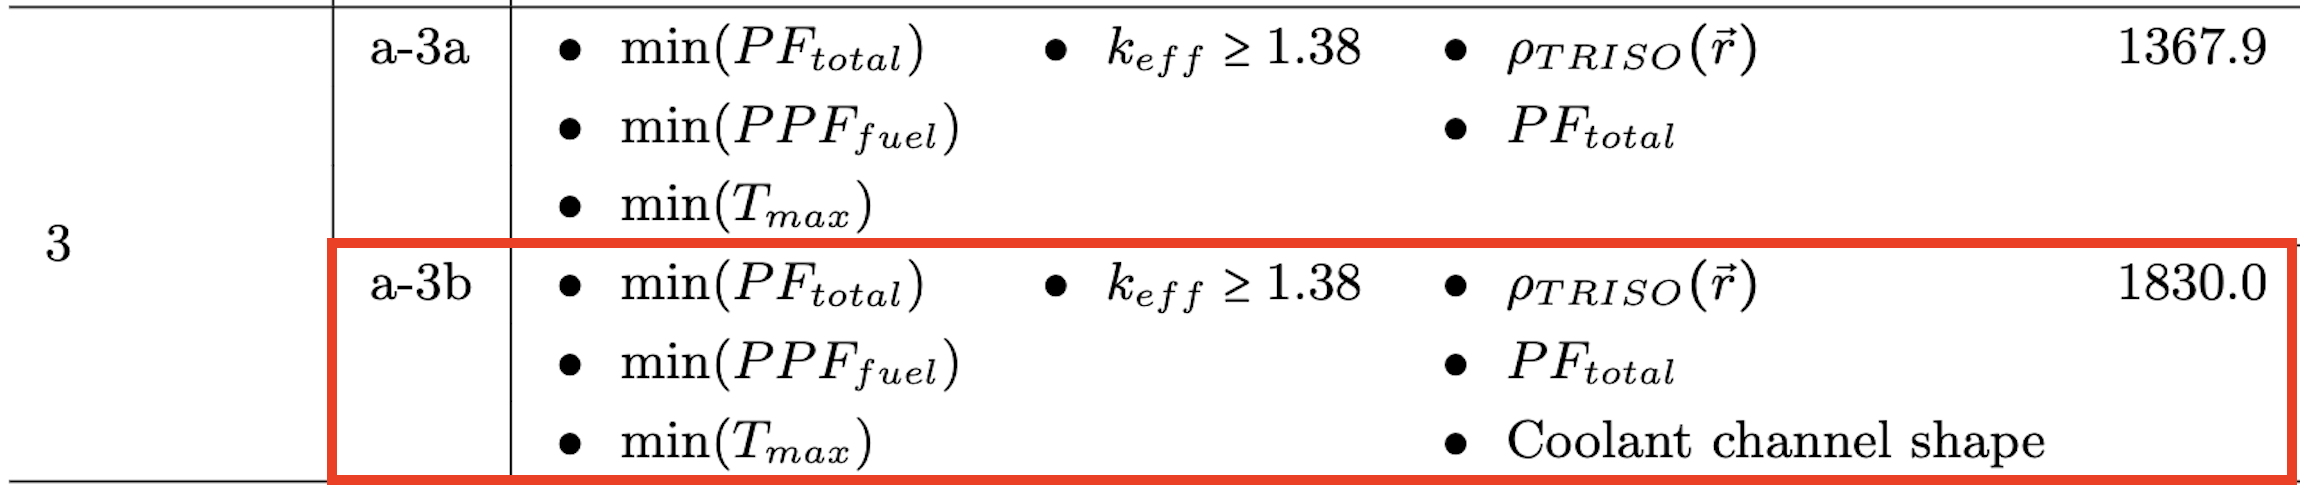
\includegraphics[width=\linewidth]{figures/ahtr-assem-opt-table-annotated3.png}
            \end{figure}

            Simulation a-3b is the \textbf{final and largest optimization problem} run 
            for the one-third assembly model that varies all input parameters to optimize 
            for all objectives. 
        }
    
\end{frame}

\begin{frame}
    \frametitle{AHTR One-Third Assembly Simulation a-1b Results}
    \visible<1->{\textbf{Simulation a-1b: I vary a, b, c, d, e f ($\rho_{TRISO}(\vec{x}, \vec{y})$)
    to minimize $T_{max}$.}} 

    \begin{figure}
        \only<1,4>{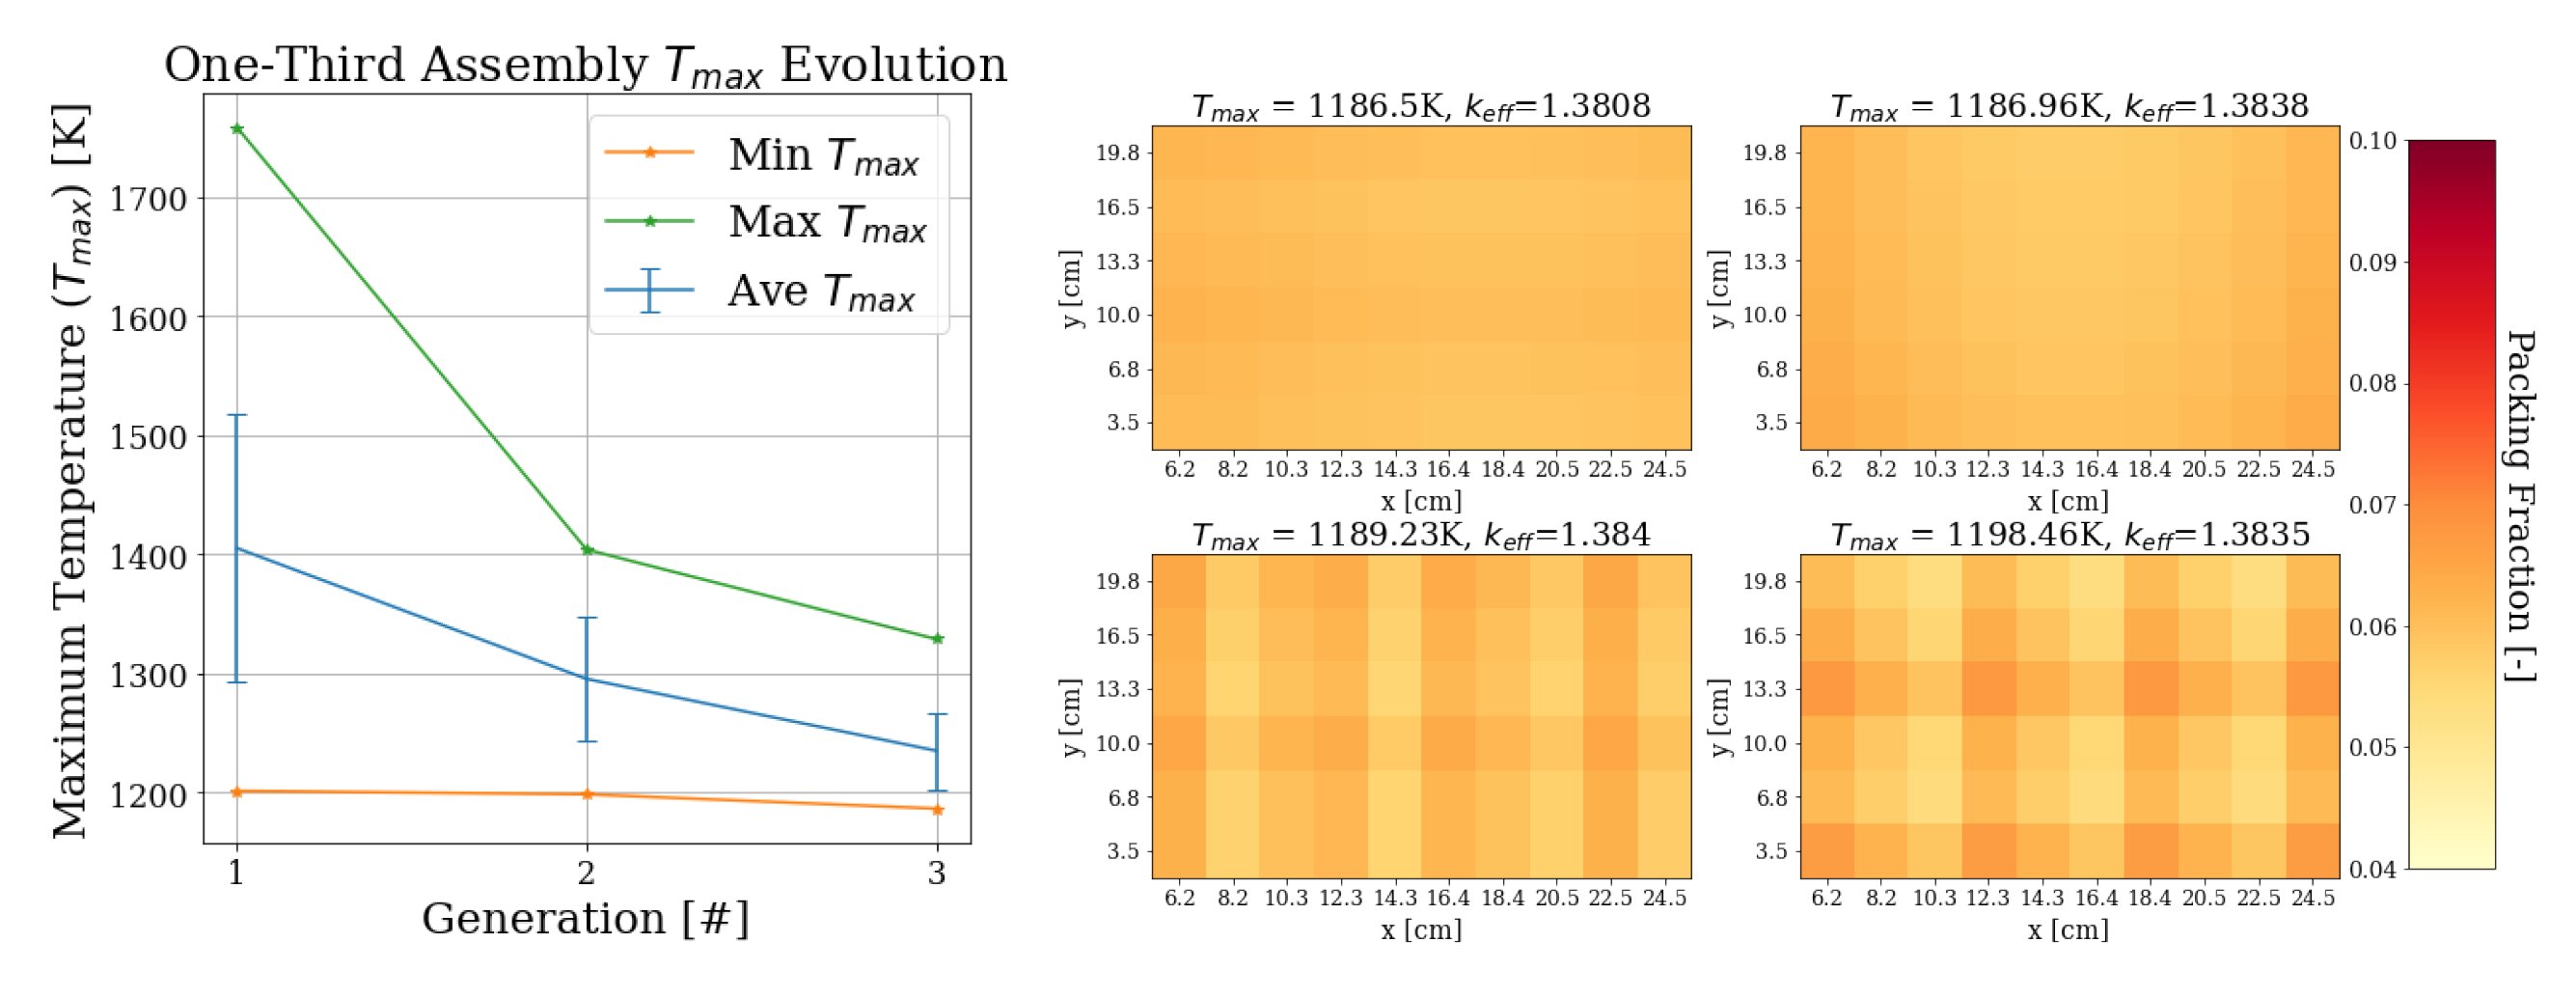
\includegraphics[width=\linewidth]{figures/assem-obj-1-temp.png}}
        \only<2>{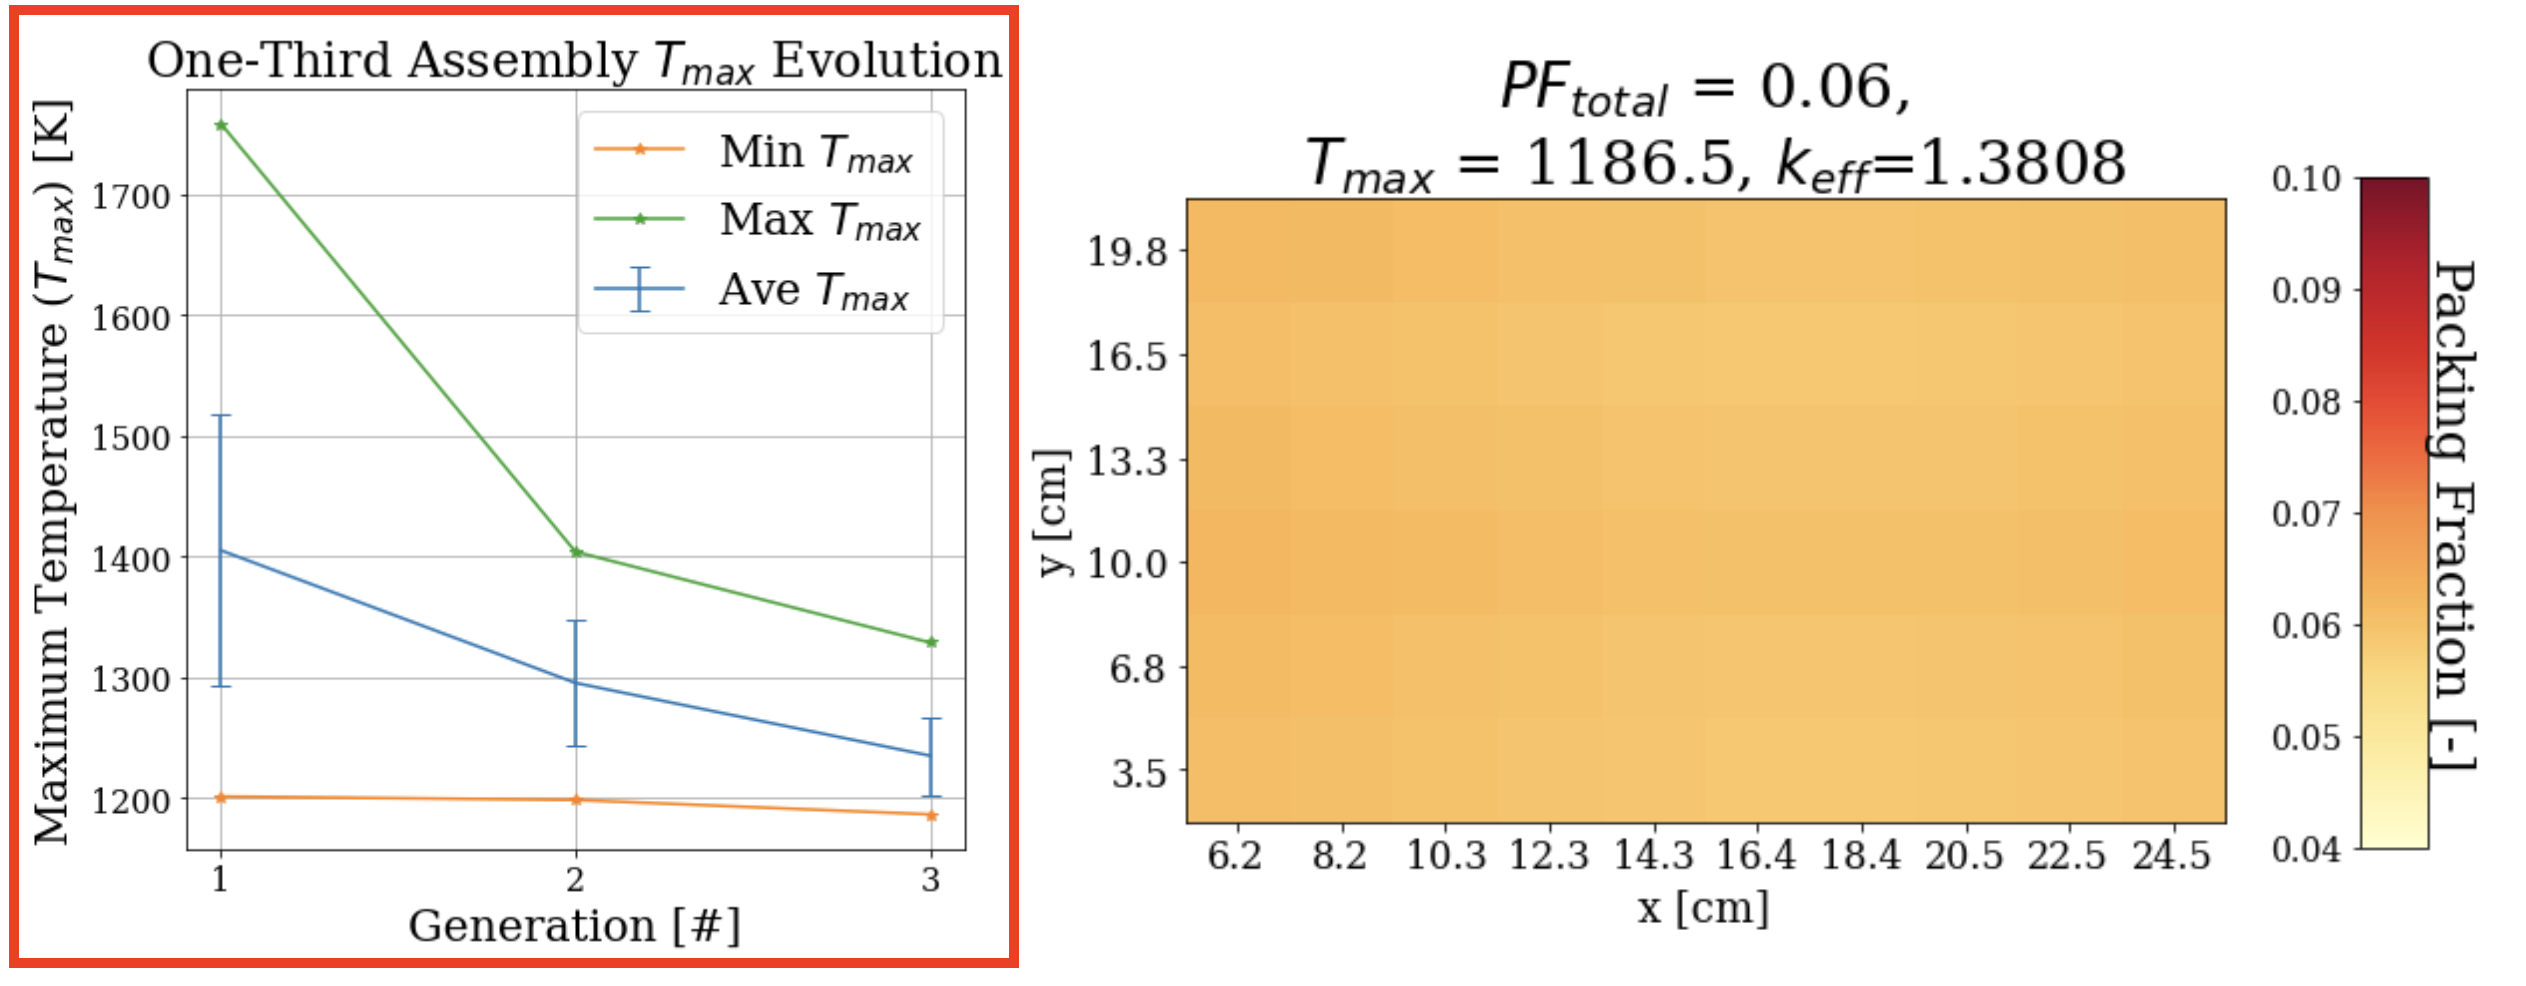
\includegraphics[width=\linewidth]{figures/assem-obj-1-temp-annotated1.png}}
        \only<3>{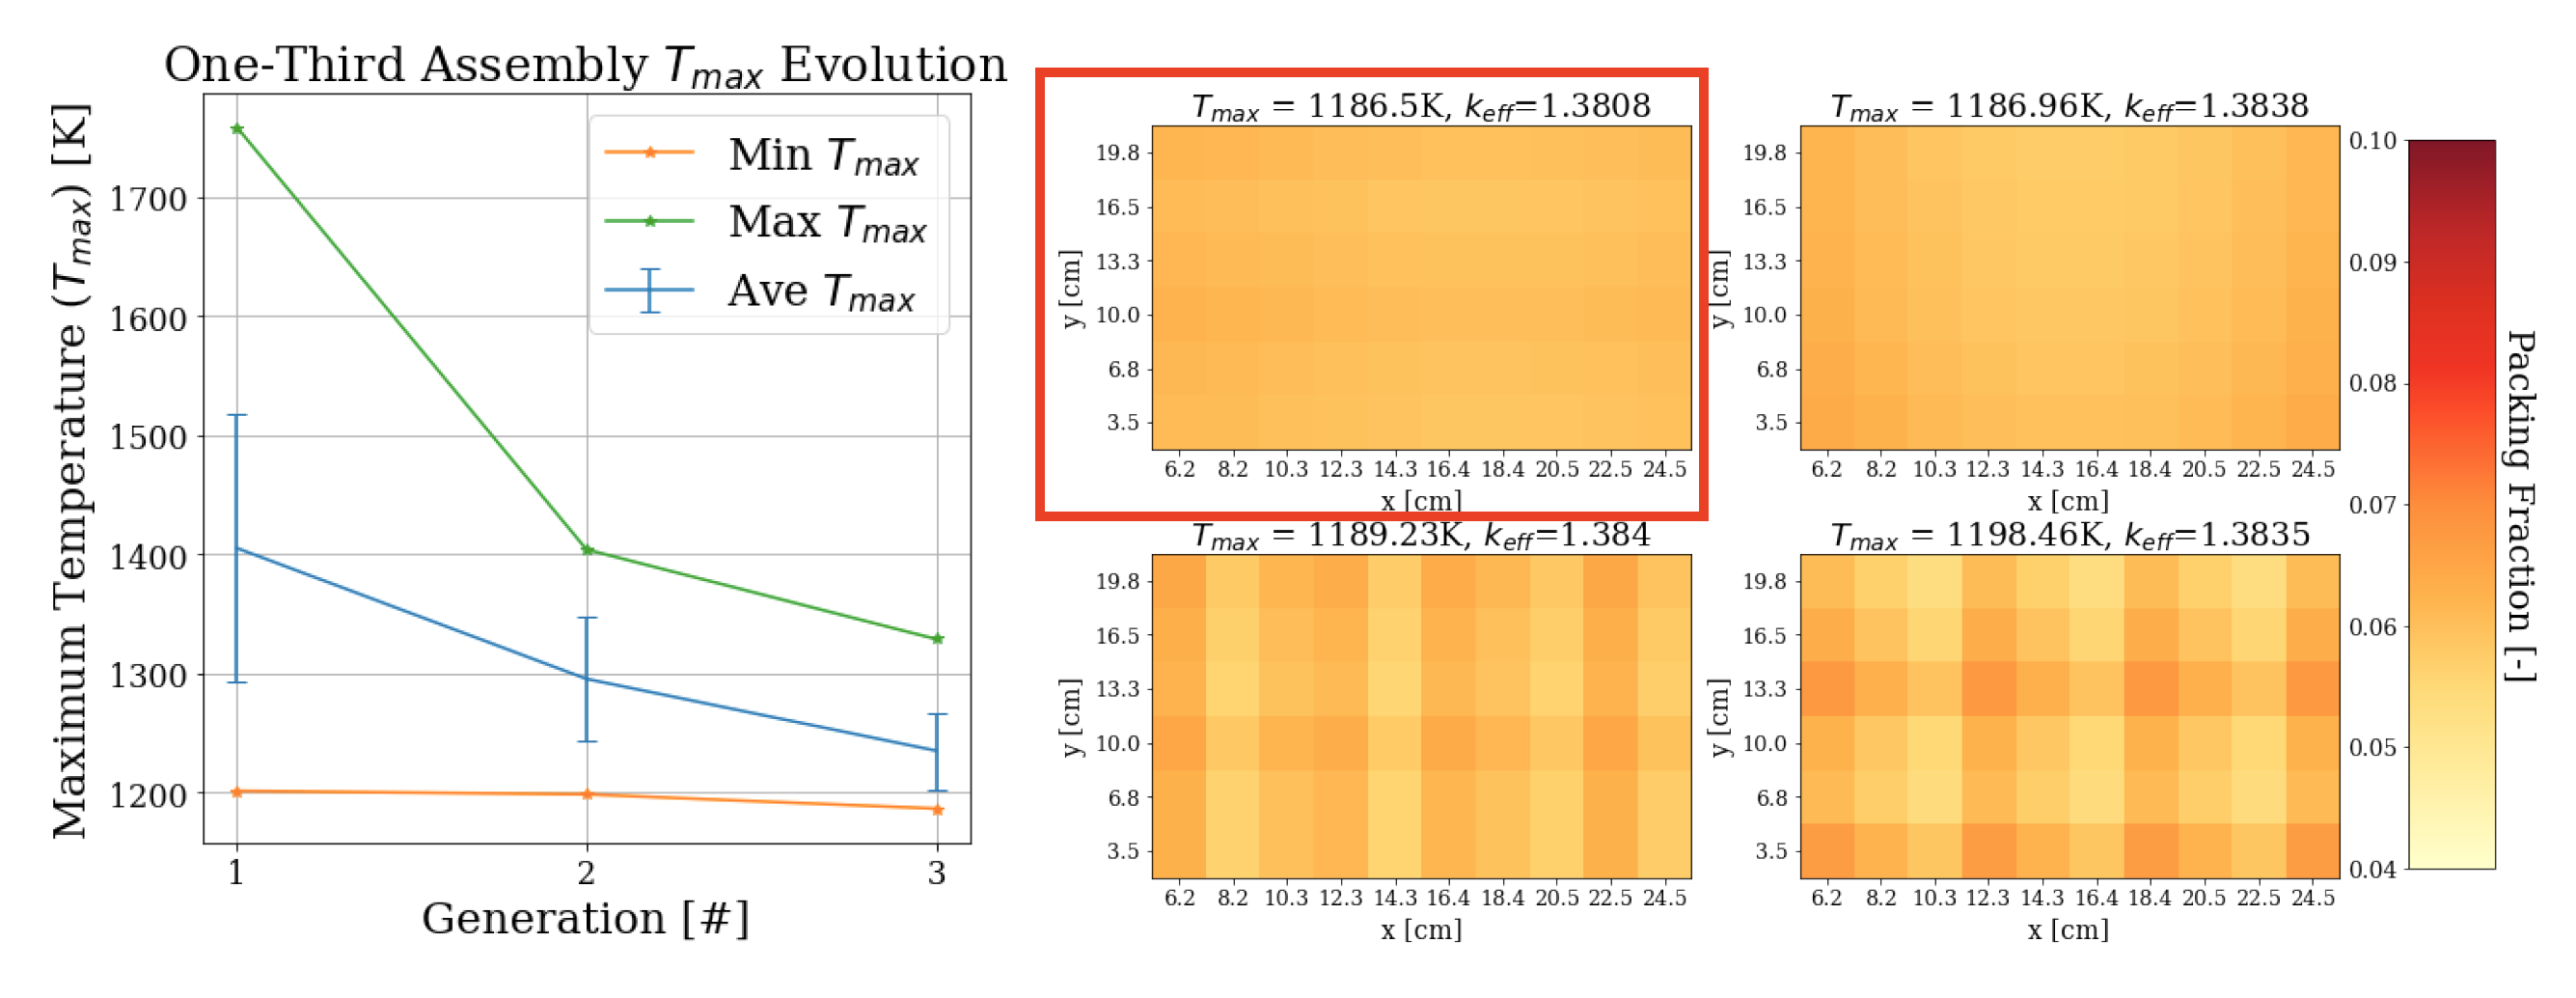
\includegraphics[width=\linewidth]{figures/assem-obj-1-temp-annotated2.png}}
        \vspace{-0.3cm}
        \caption{Simulation a-1b $T_{max}$ evolution and TRISO distribution with lowest 
        $T_{max}$.}
    \end{figure}

    \only<2>{
    \vspace{-0.2cm}
    Simulation a-1b runs for 3 generations with 128 reactor models per 
    generation, the average $T_{max}$ decreased by $\approx$ 100K per generation. 

    \textbf{The average one-third assembly $T_{max}$ converged to $\approx$ 1220K}.}

    \only<3>{\textbf{The TRISO distribution in the final generation with the 
    lowest $T_{max}$ has $T_{max}$ = 1186K and an almost constant TRISO packing fraction 
    distribution.}}

    \only<4>{
    \vspace{-0.4cm}    
    \begin{tcolorbox}[colback=illiniorange,colframe=illiniorange!50!black]
        \textbf{A flatter TRISO distribution minimizes $T_{max}$.}
    \end{tcolorbox}}
\end{frame}

\begin{frame}
    \frametitle{AHTR One-Third Assembly Simulation a-1e Results}
    \visible<1->{\textbf{I vary $r_1, r_2, r_3, r_4, r_5$ (coolant channel shape)
    to minimize $T_{max}$.}}

    \begin{figure}
        \centering
        \begin{subfigure}{0.3\textwidth}
            \only<1,3>{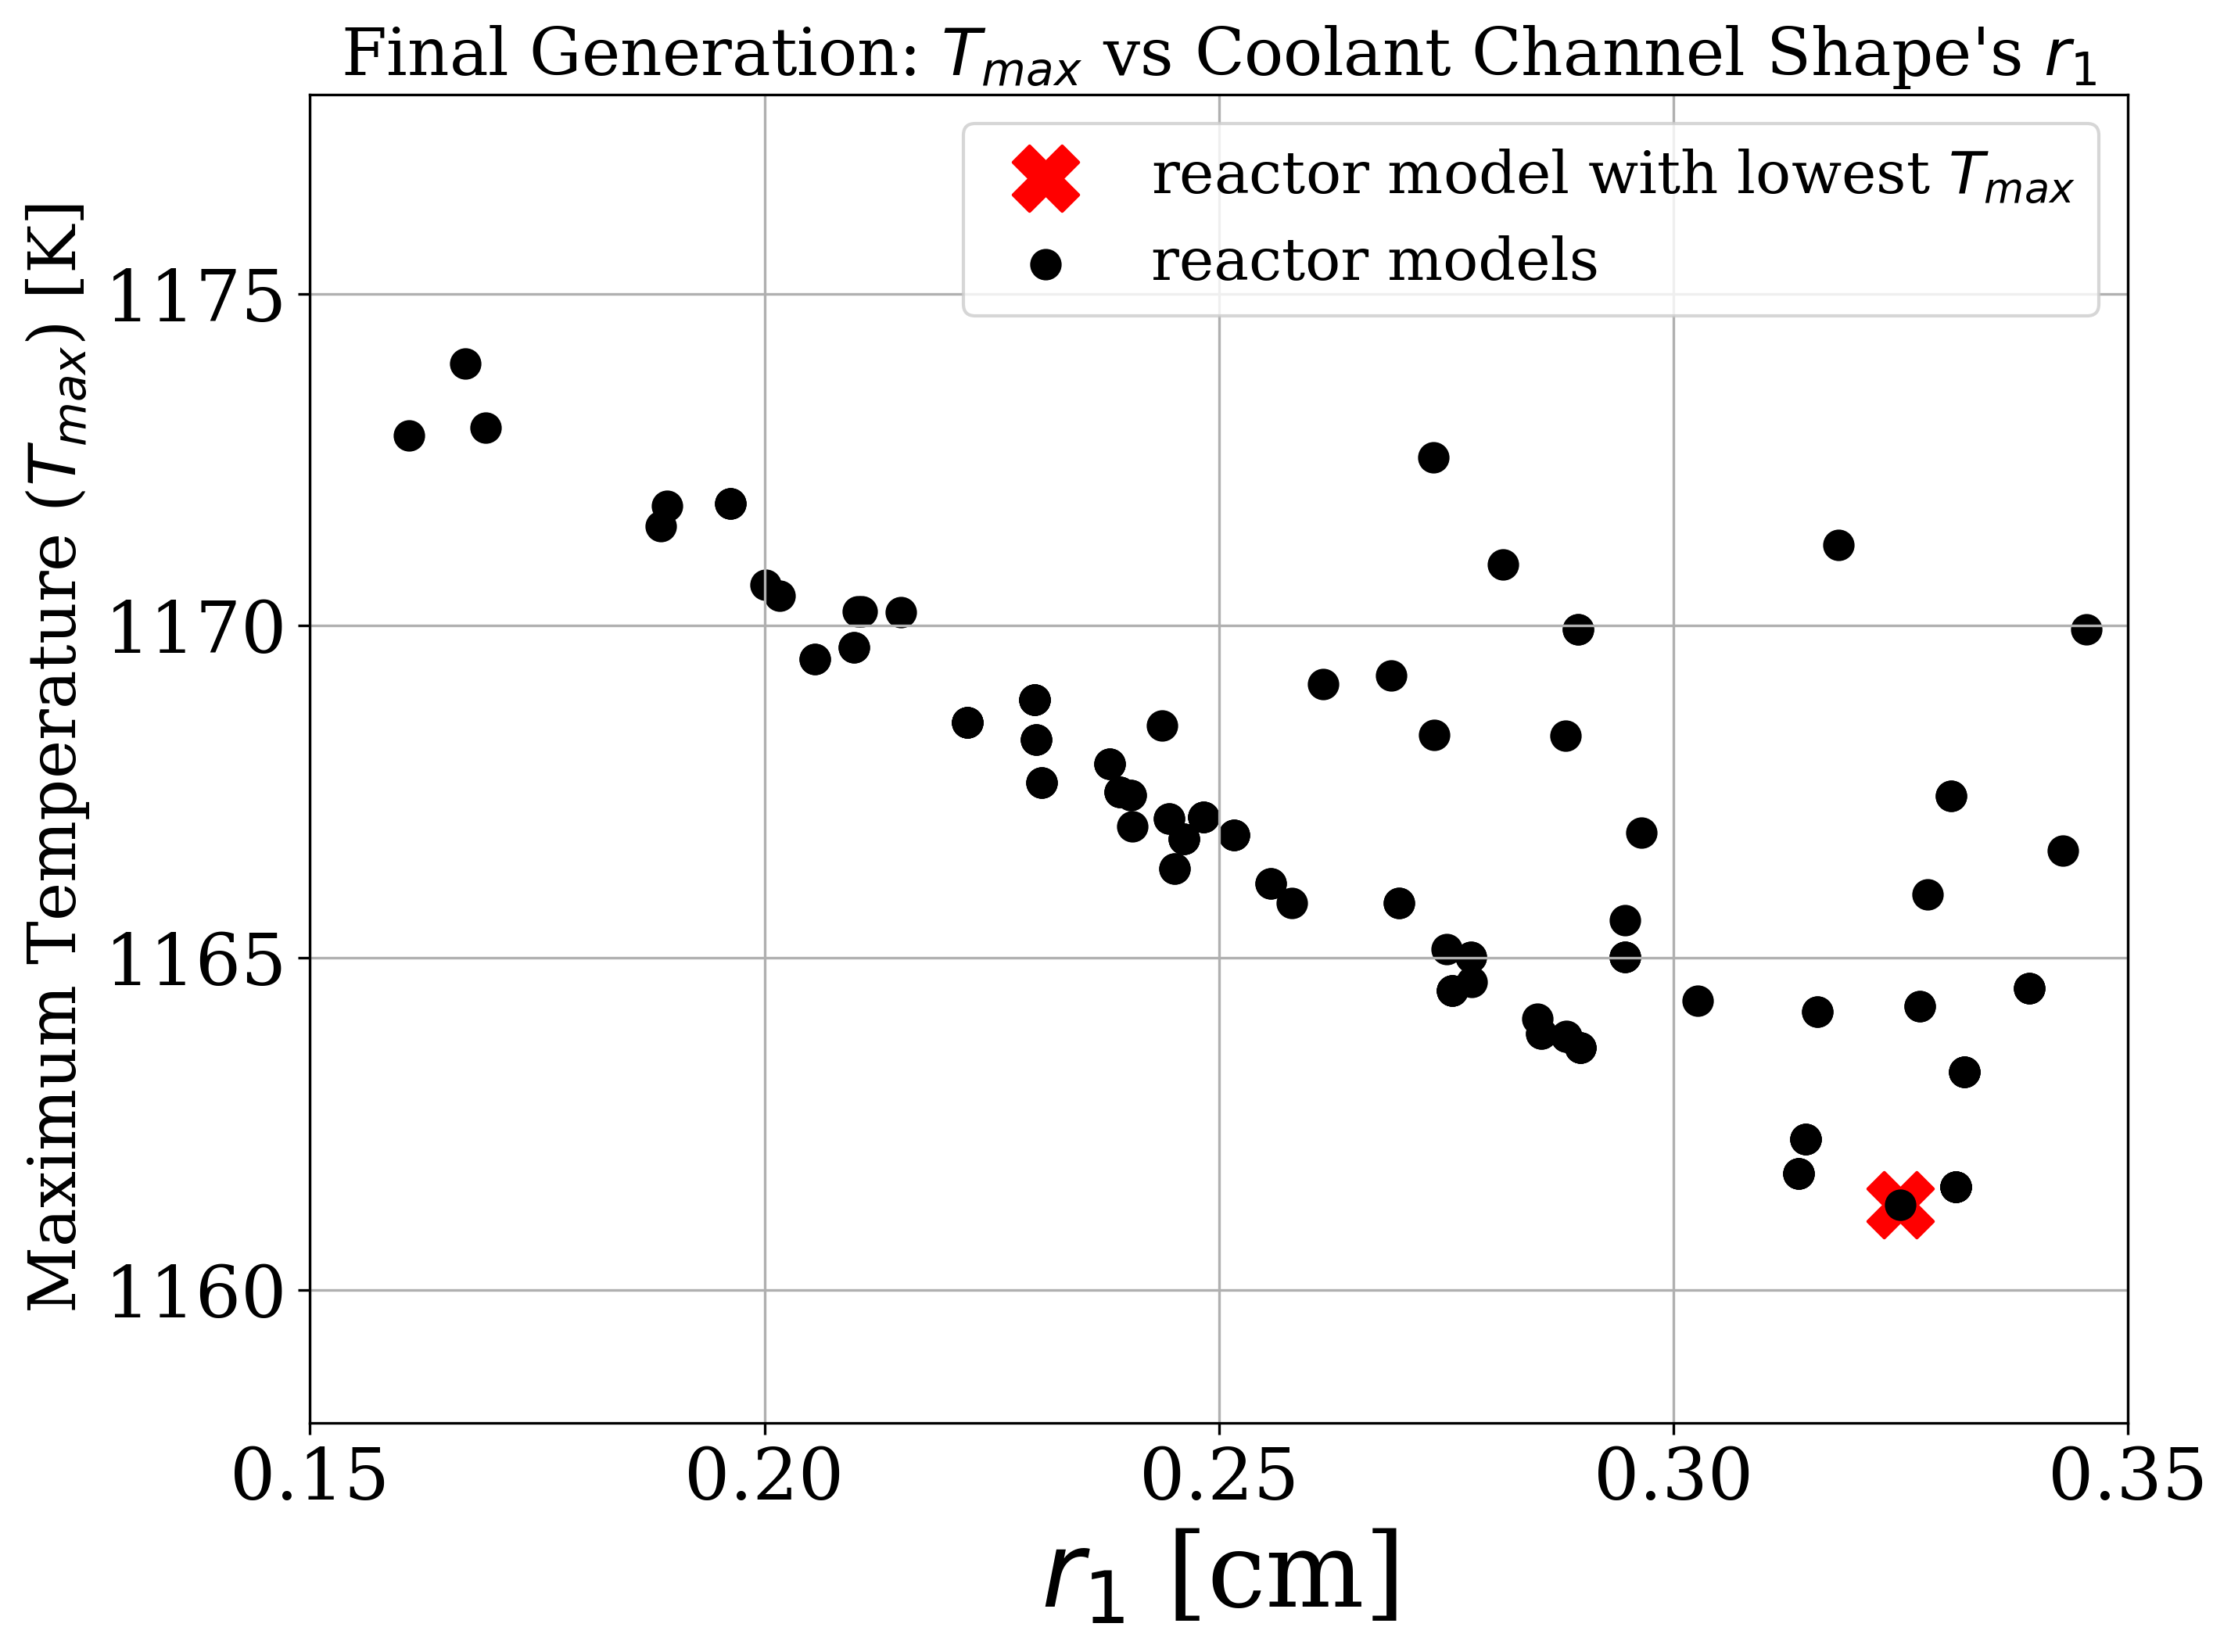
\includegraphics[width=\linewidth]{figures/a-1e-r1-pres.png}}
            \only<2>{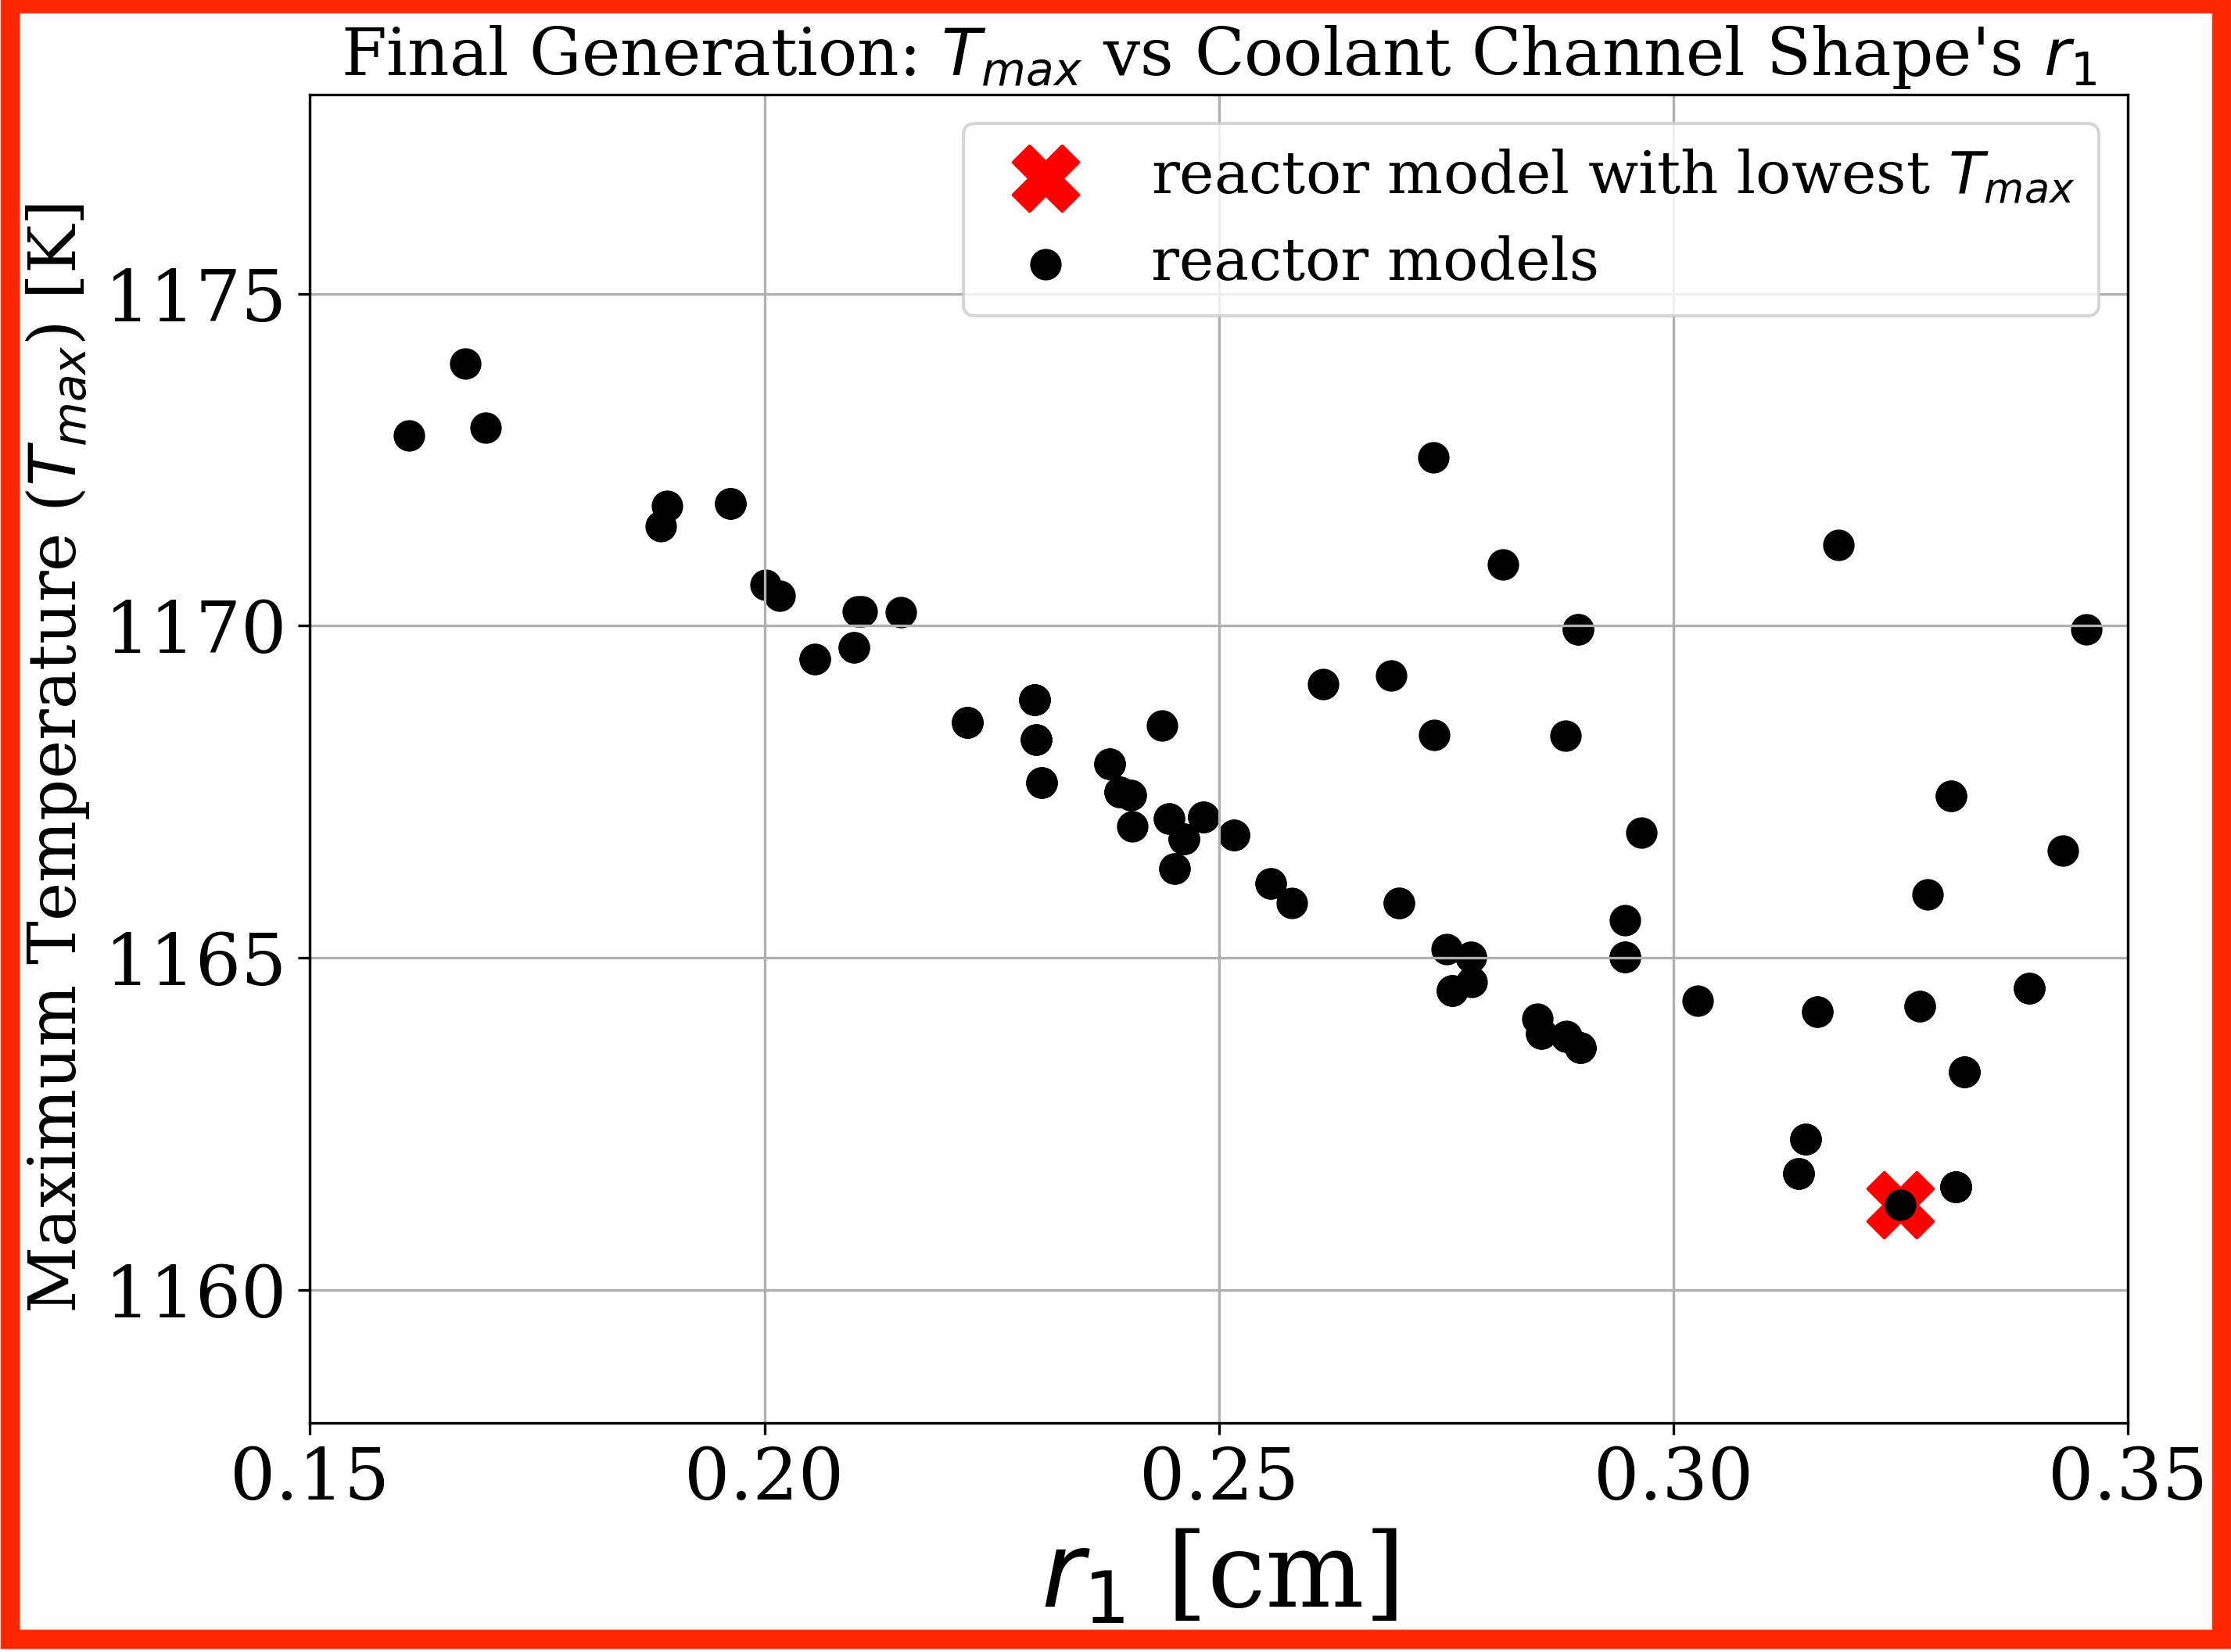
\includegraphics[width=\linewidth]{figures/a-1e-r1-pres-annotated.png}}
            \vspace{-0.5cm}
            \caption{Plot of $T_{max}$ against $r_1$.}
        \end{subfigure}
        \begin{subfigure}{0.3\textwidth}
            \only<1,2>{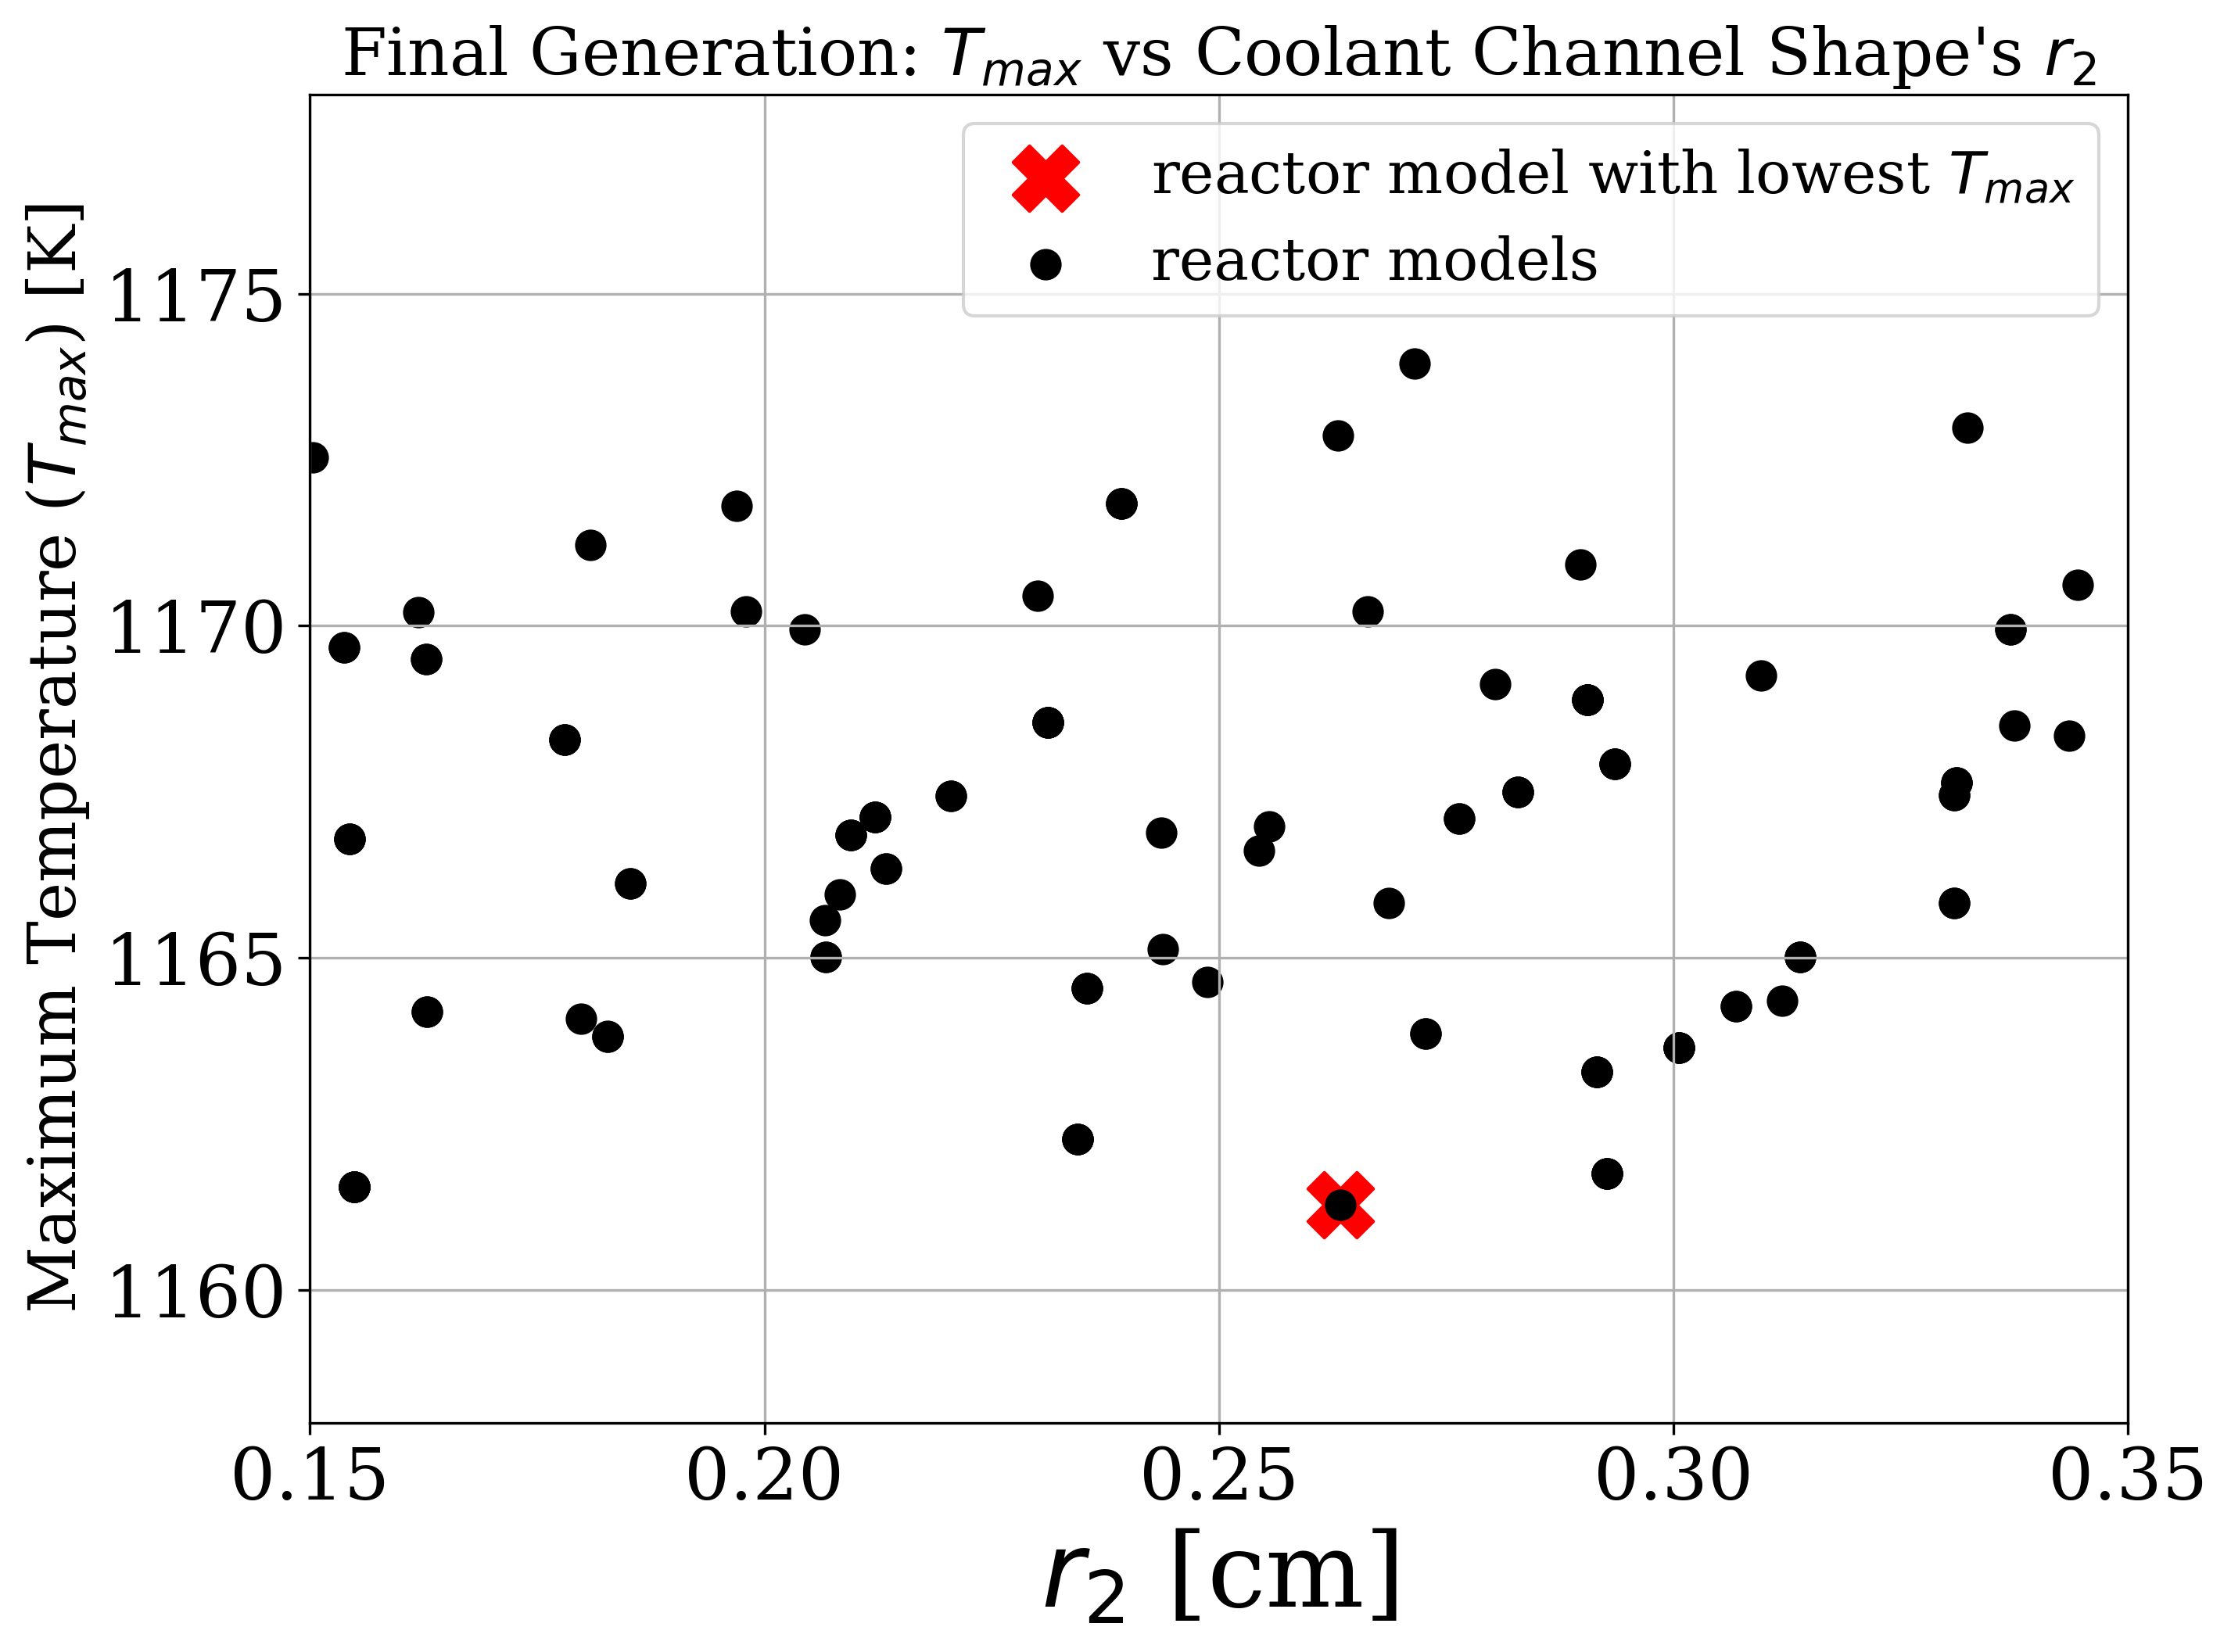
\includegraphics[width=\linewidth]{figures/a-1e-r2-pres.png}}
            \only<3>{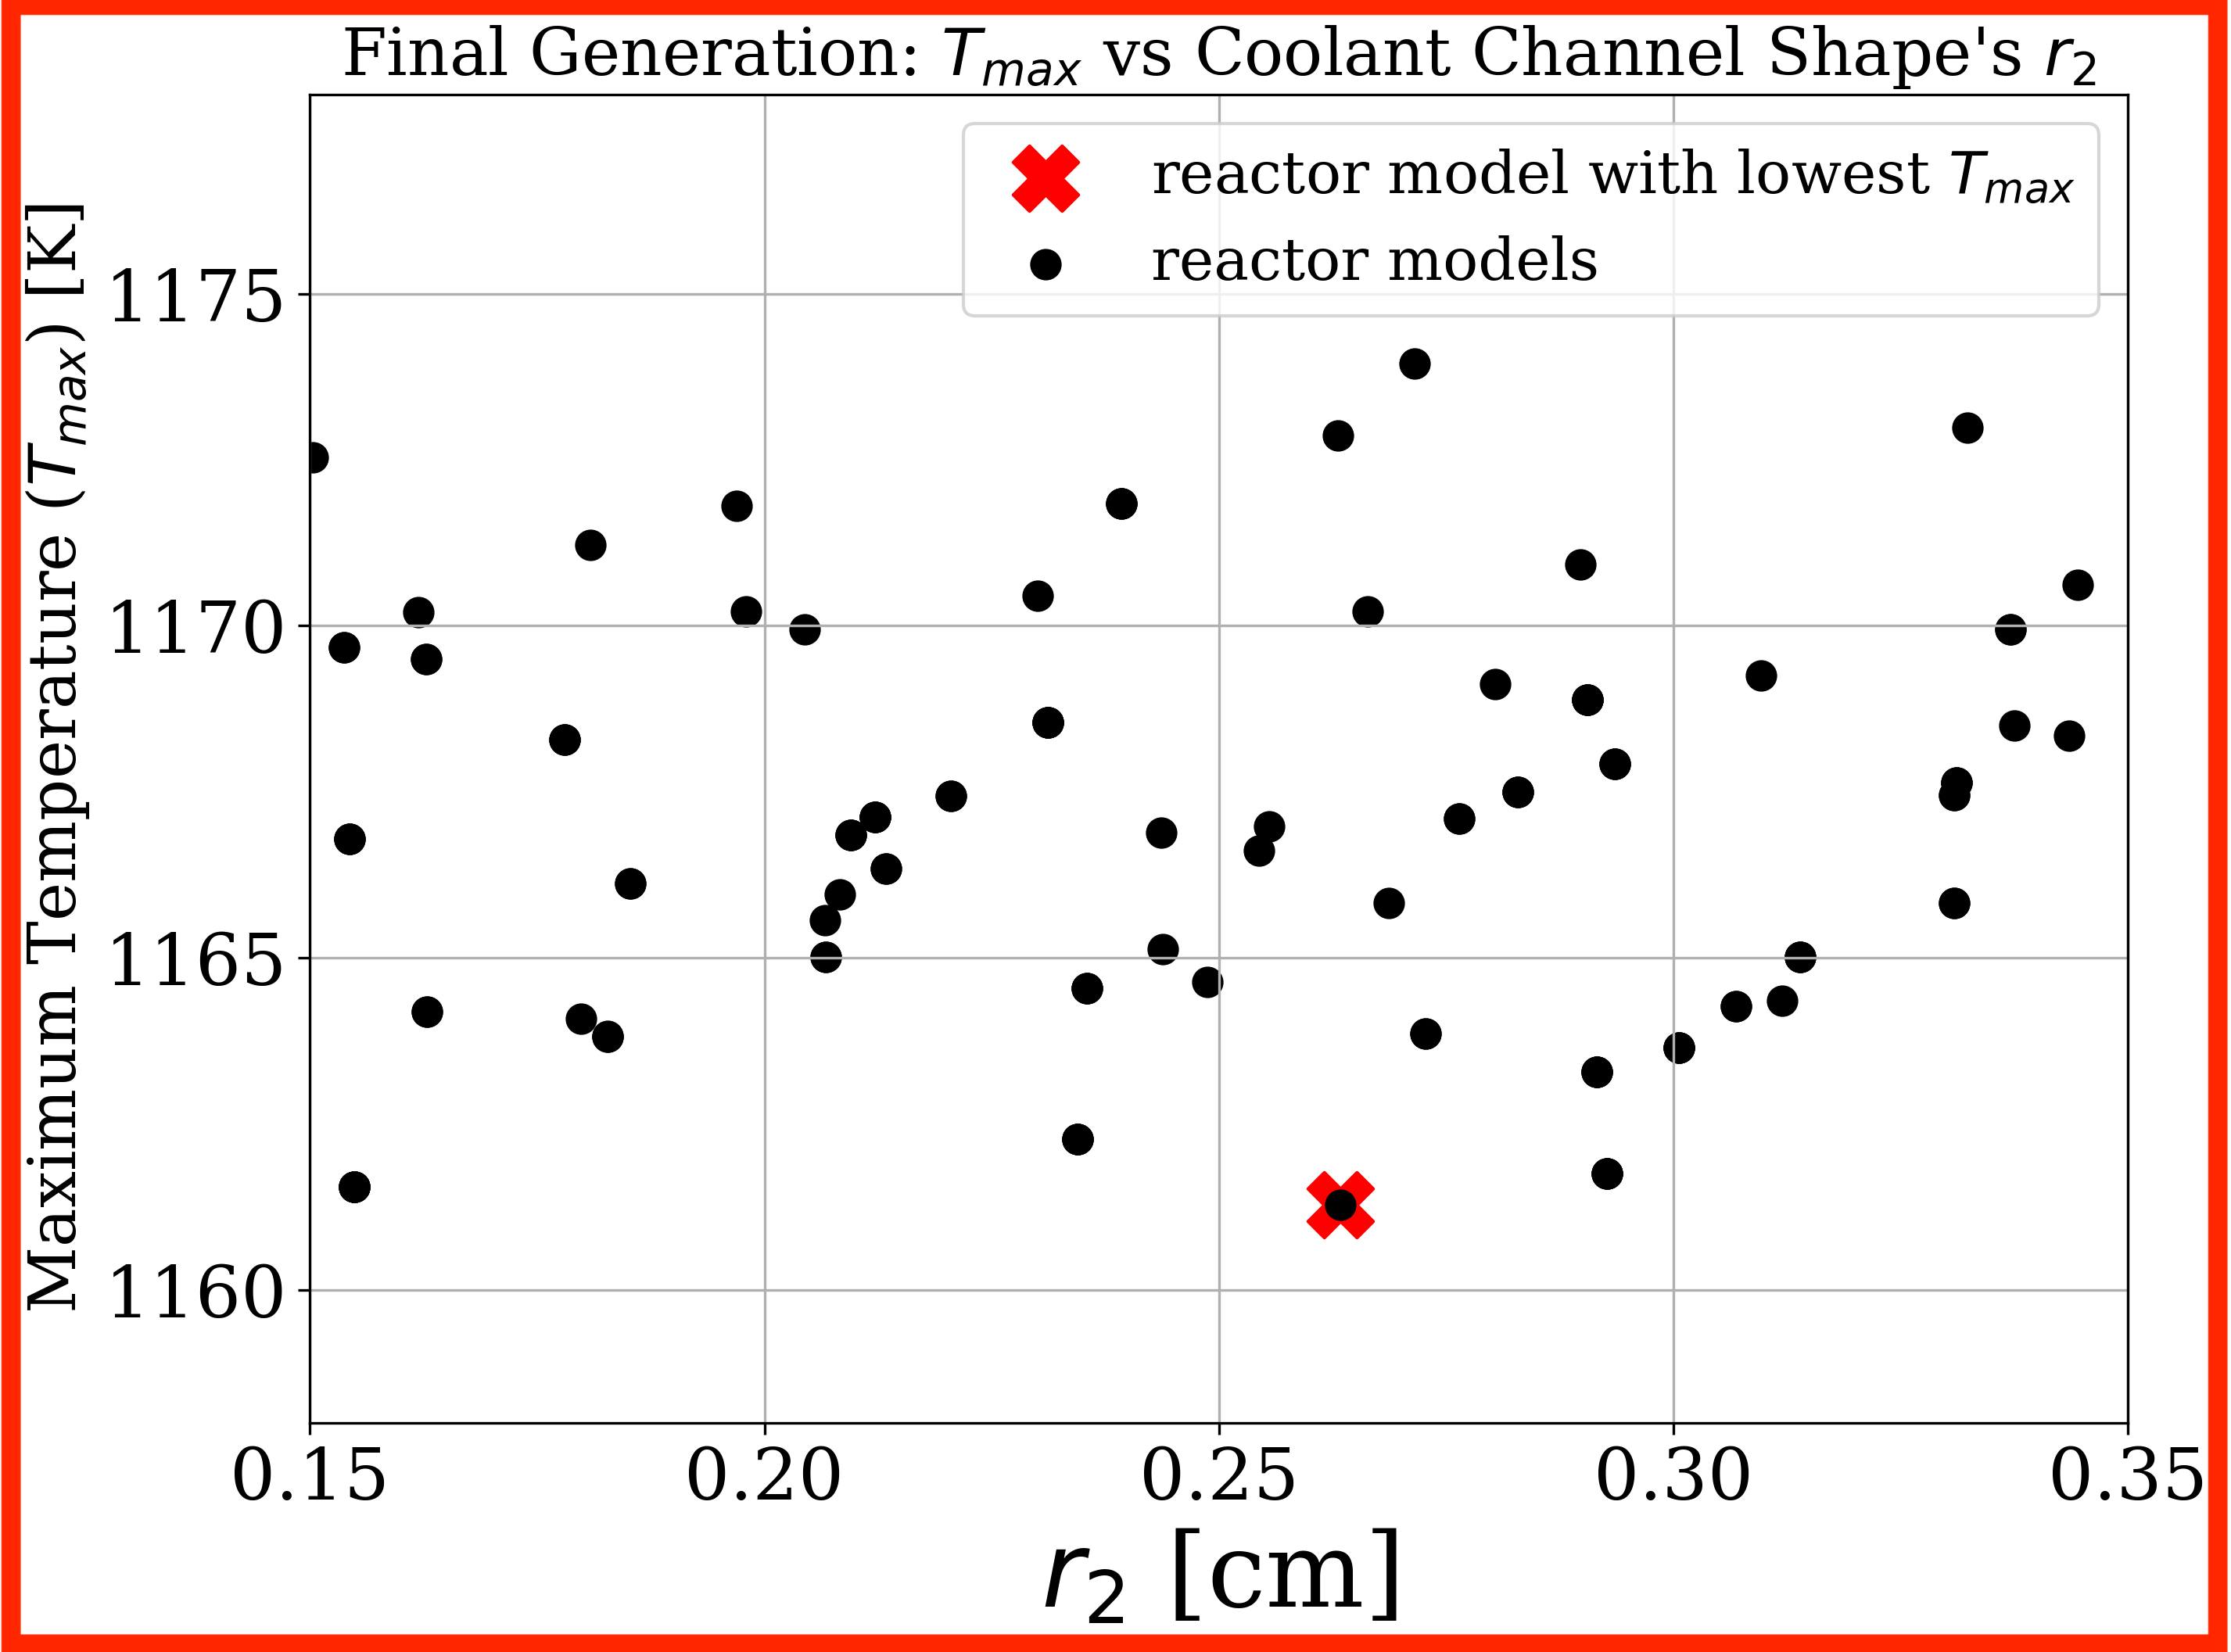
\includegraphics[width=\linewidth]{figures/a-1e-r2-pres-annotated.png}}
            \vspace{-0.5cm}
            \caption{Plot of $T_{max}$ against $r_2$.}
        \end{subfigure}
        \begin{subfigure}{0.3\textwidth}
            \only<1,2>{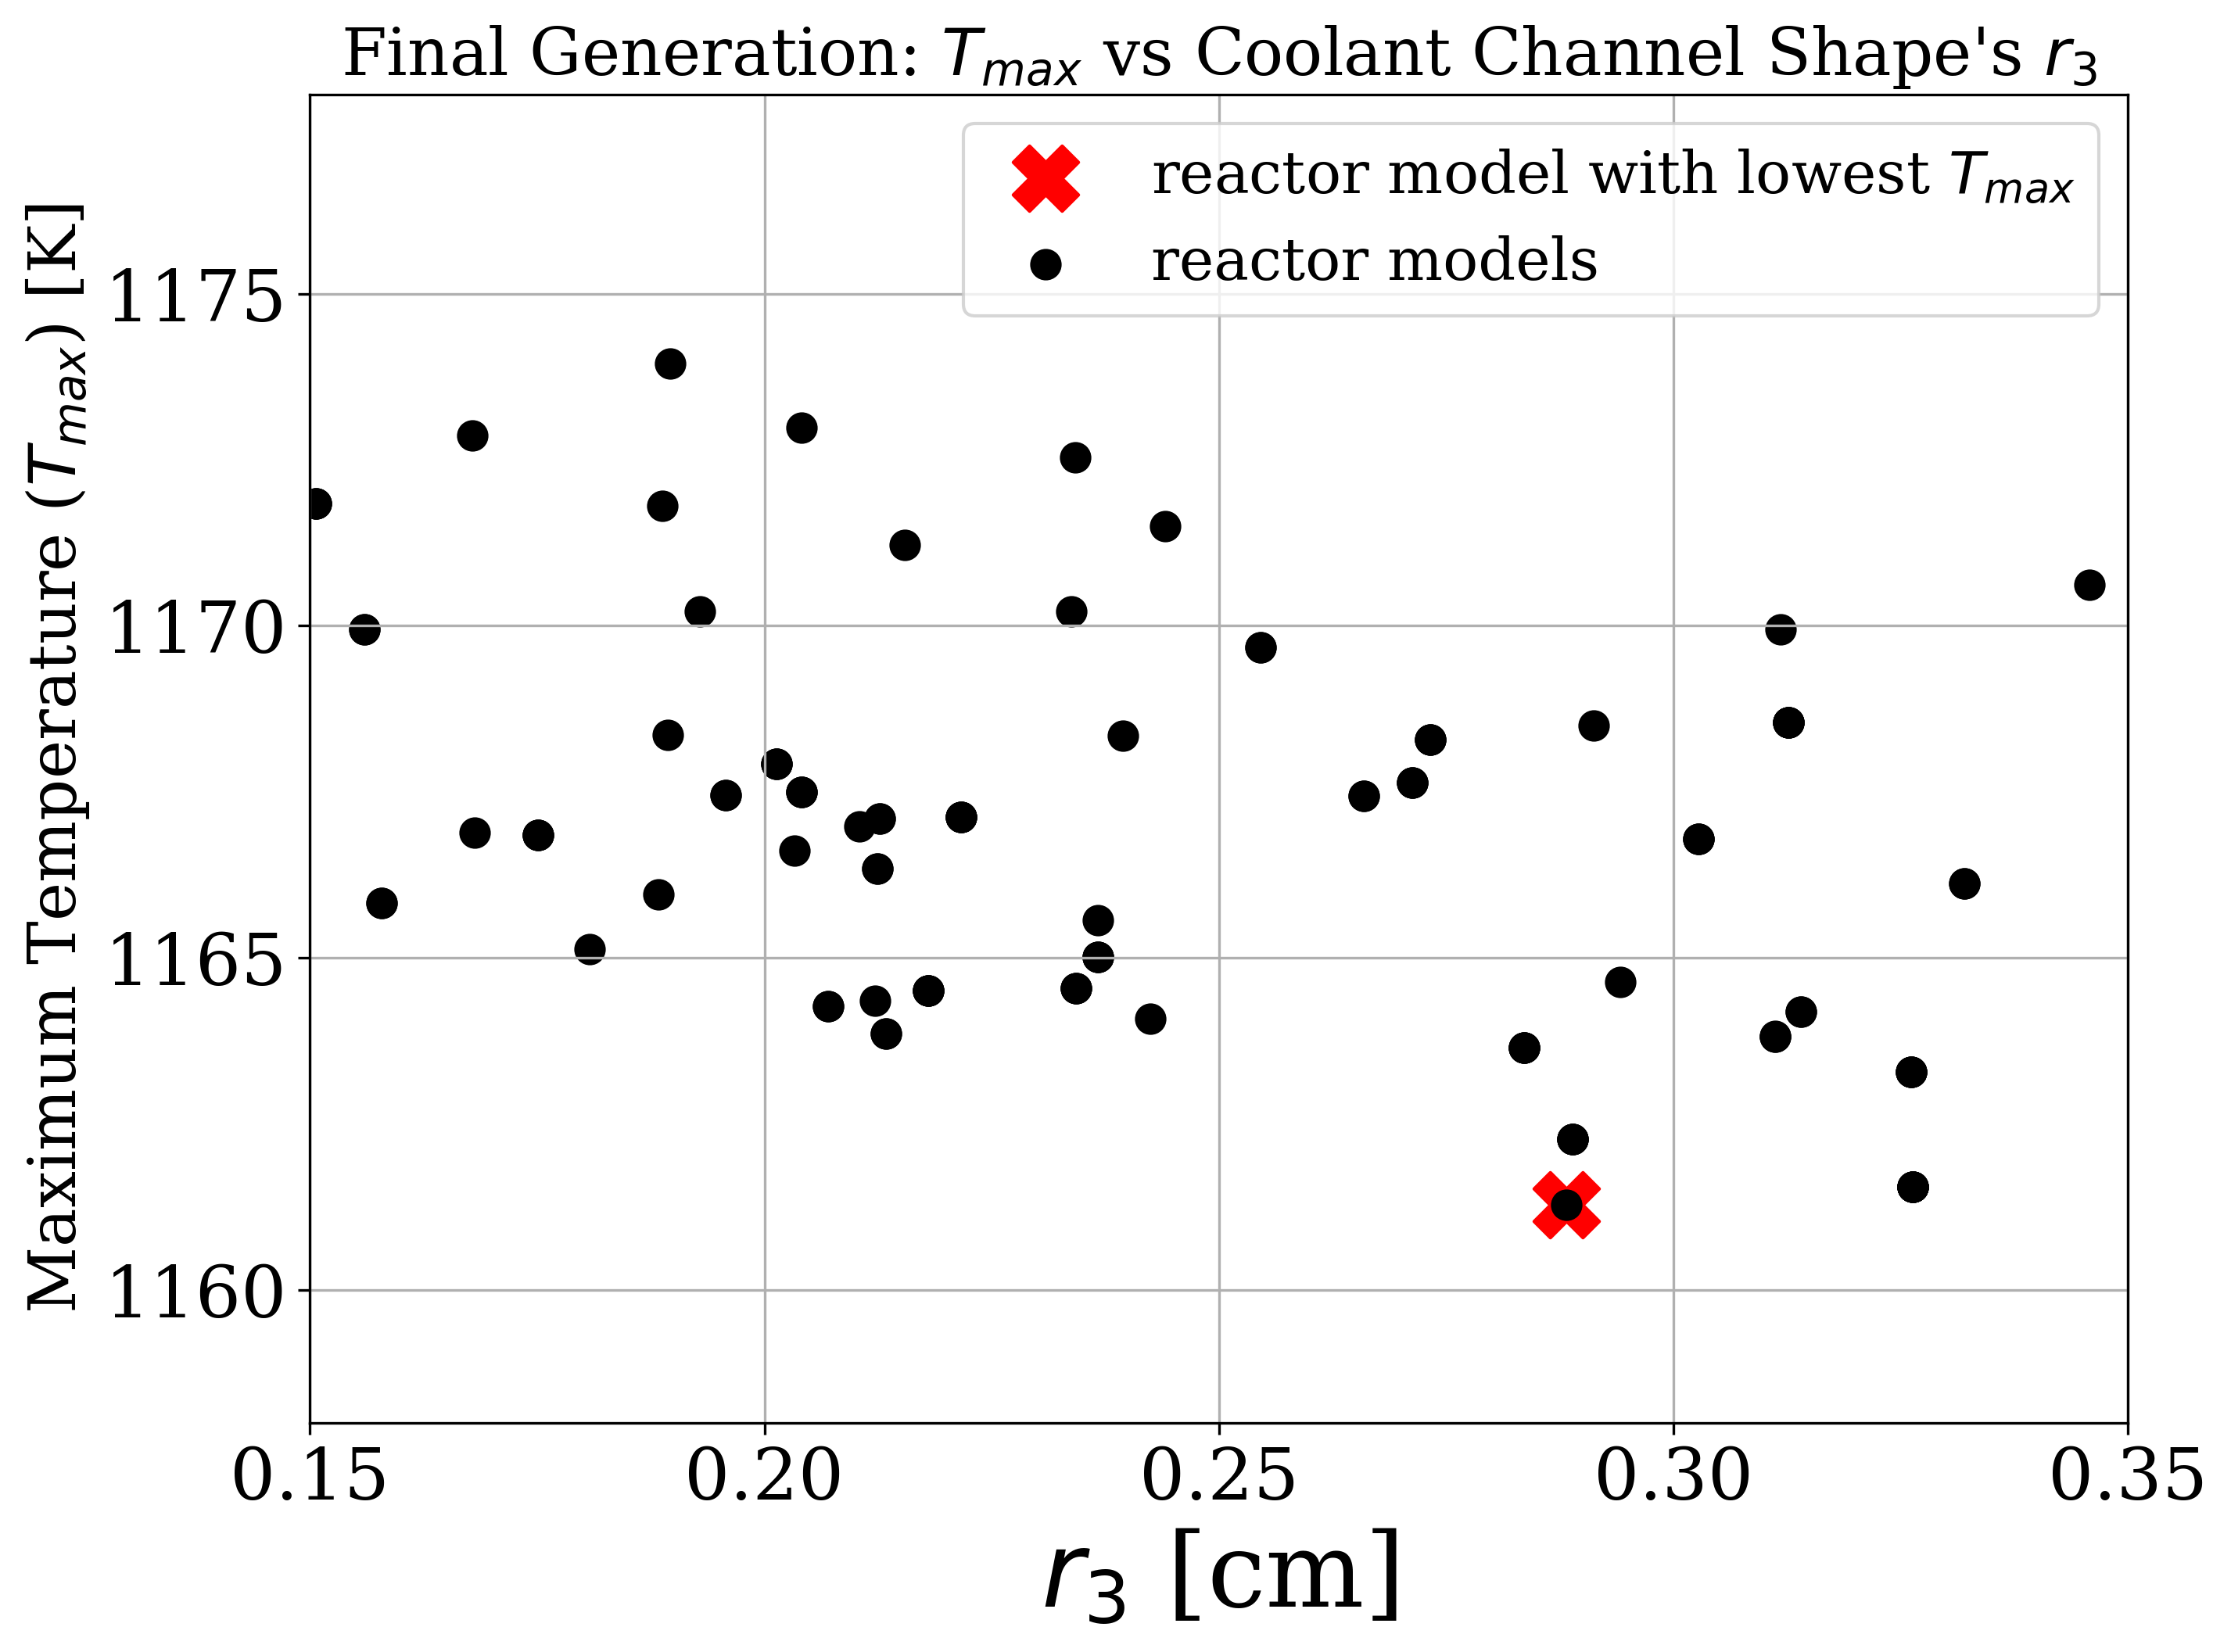
\includegraphics[width=\linewidth]{figures/a-1e-r3-pres.png}}
            \only<3>{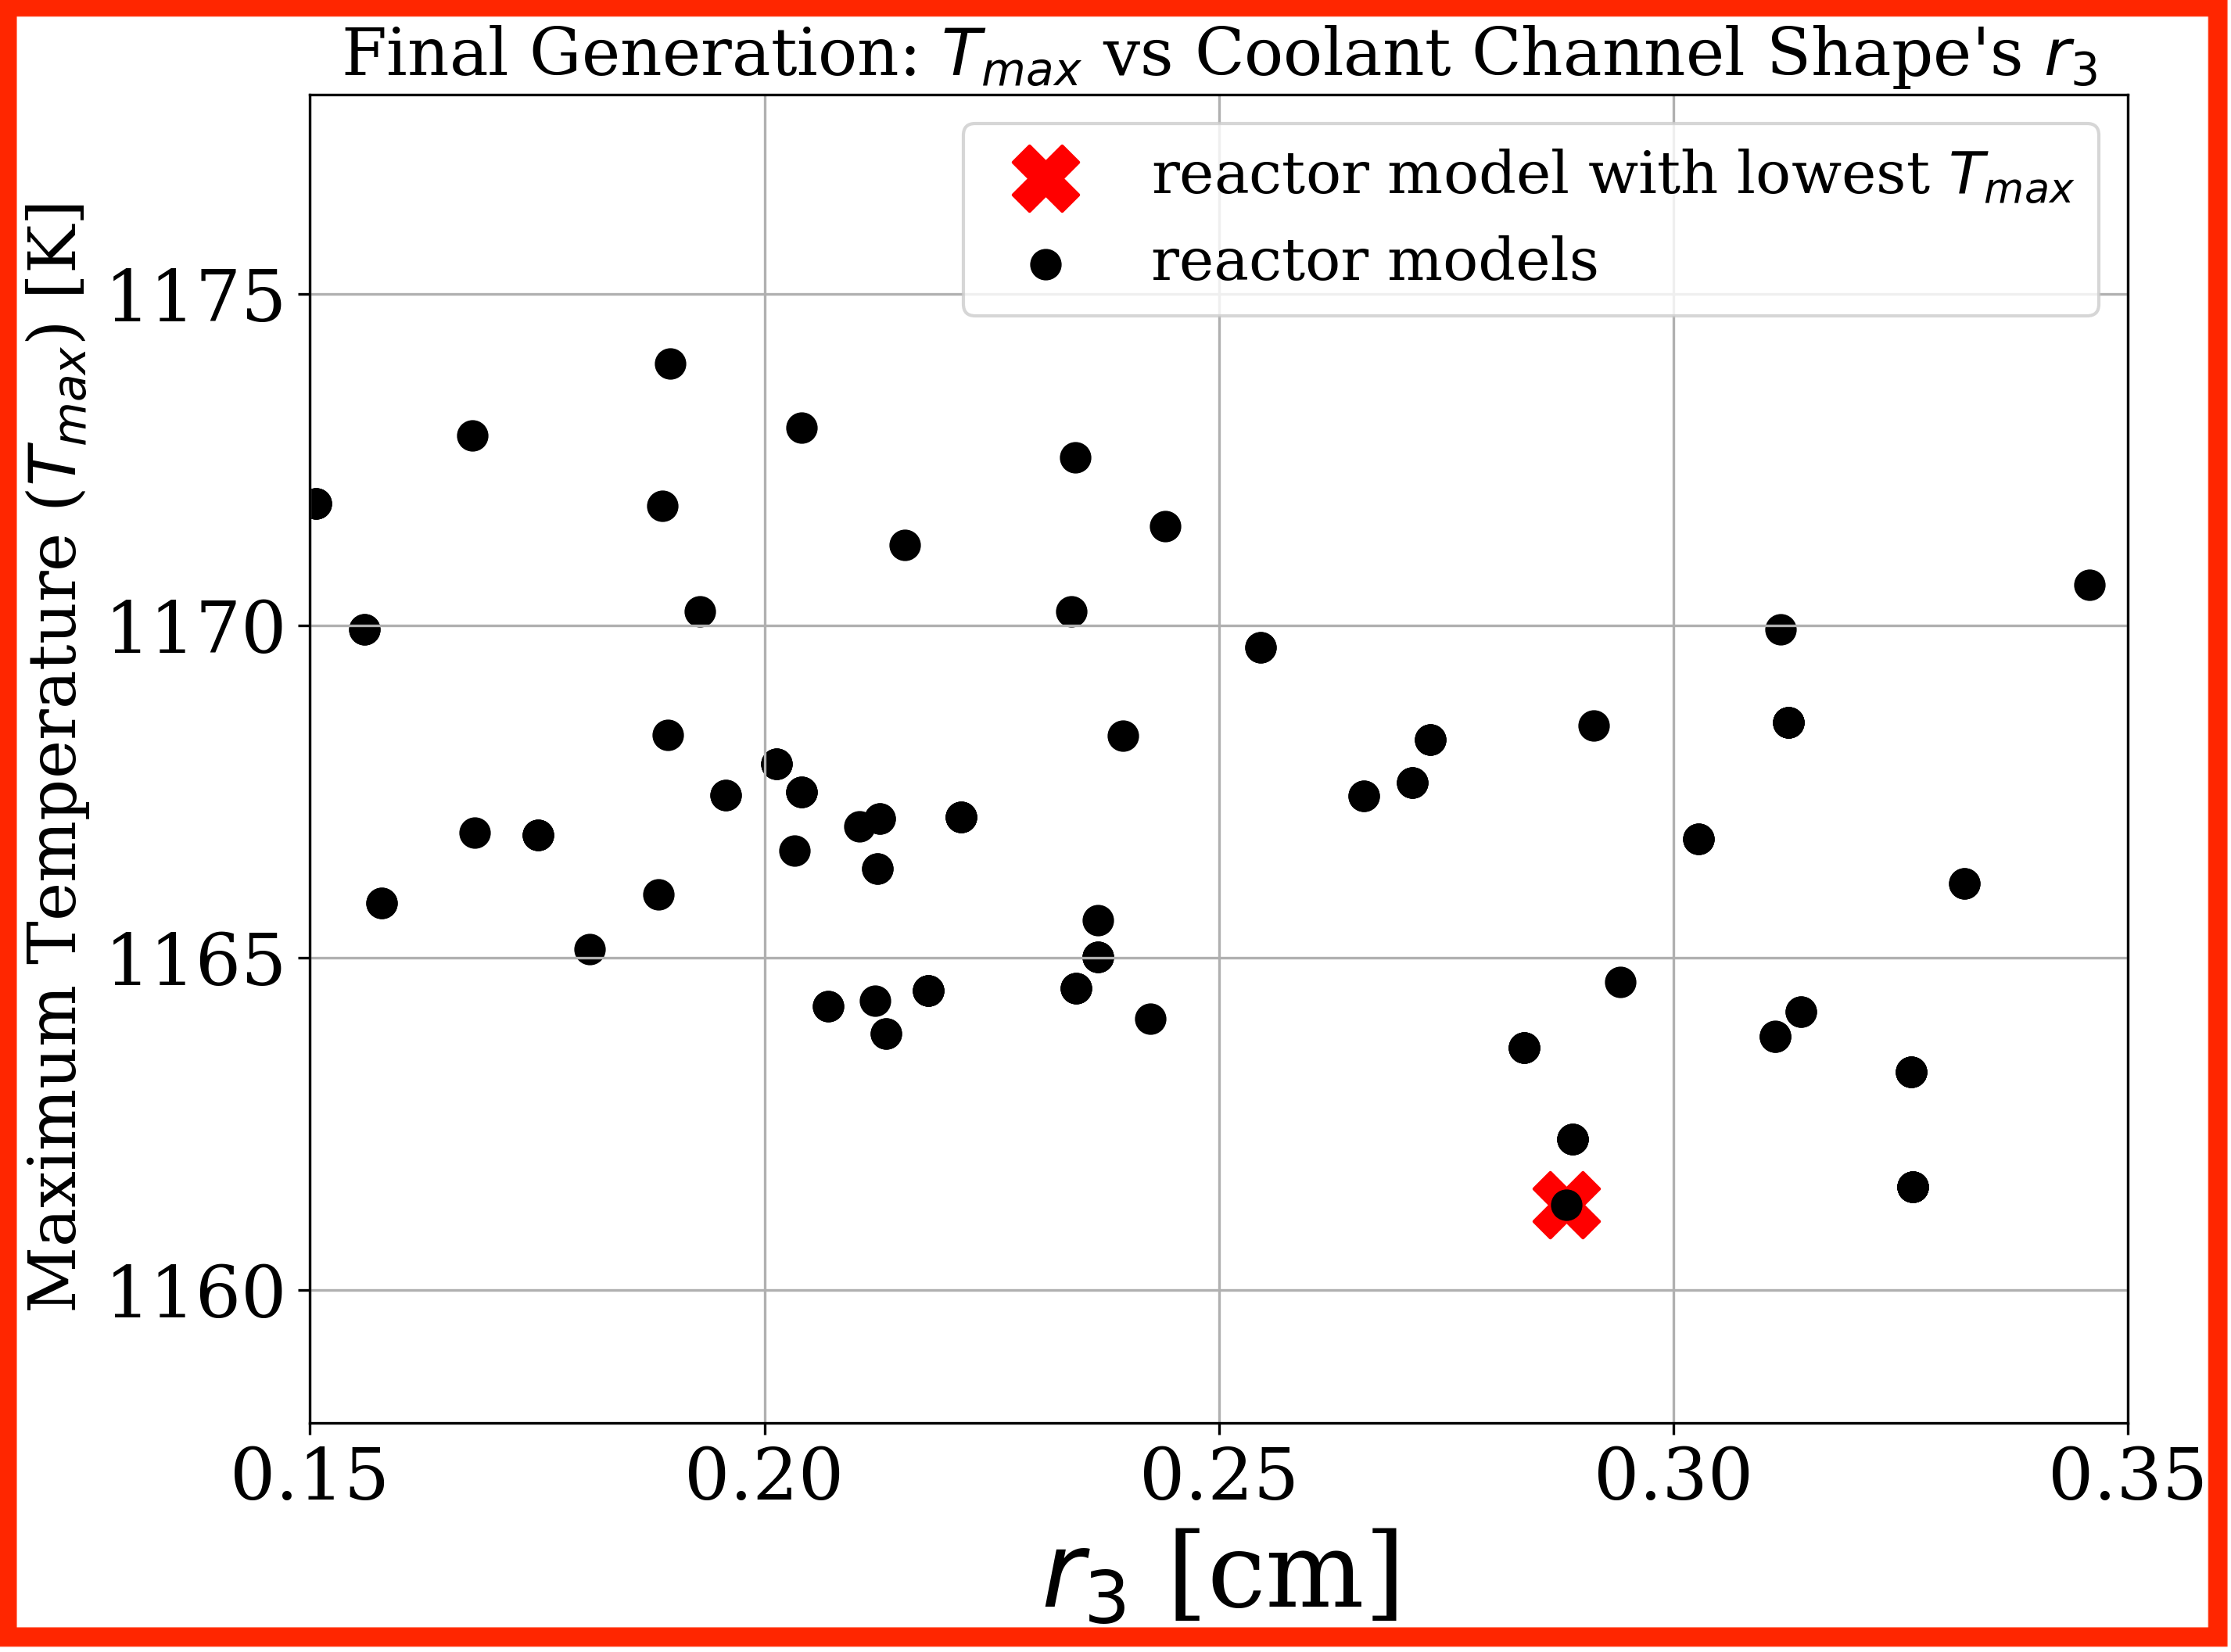
\includegraphics[width=\linewidth]{figures/a-1e-r3-pres-annotated.png}}
            \vspace{-0.5cm}
            \caption{Plot of $T_{max}$ against $r_3$.}
        \end{subfigure}
        \begin{subfigure}{0.3\textwidth}
            \only<1,2>{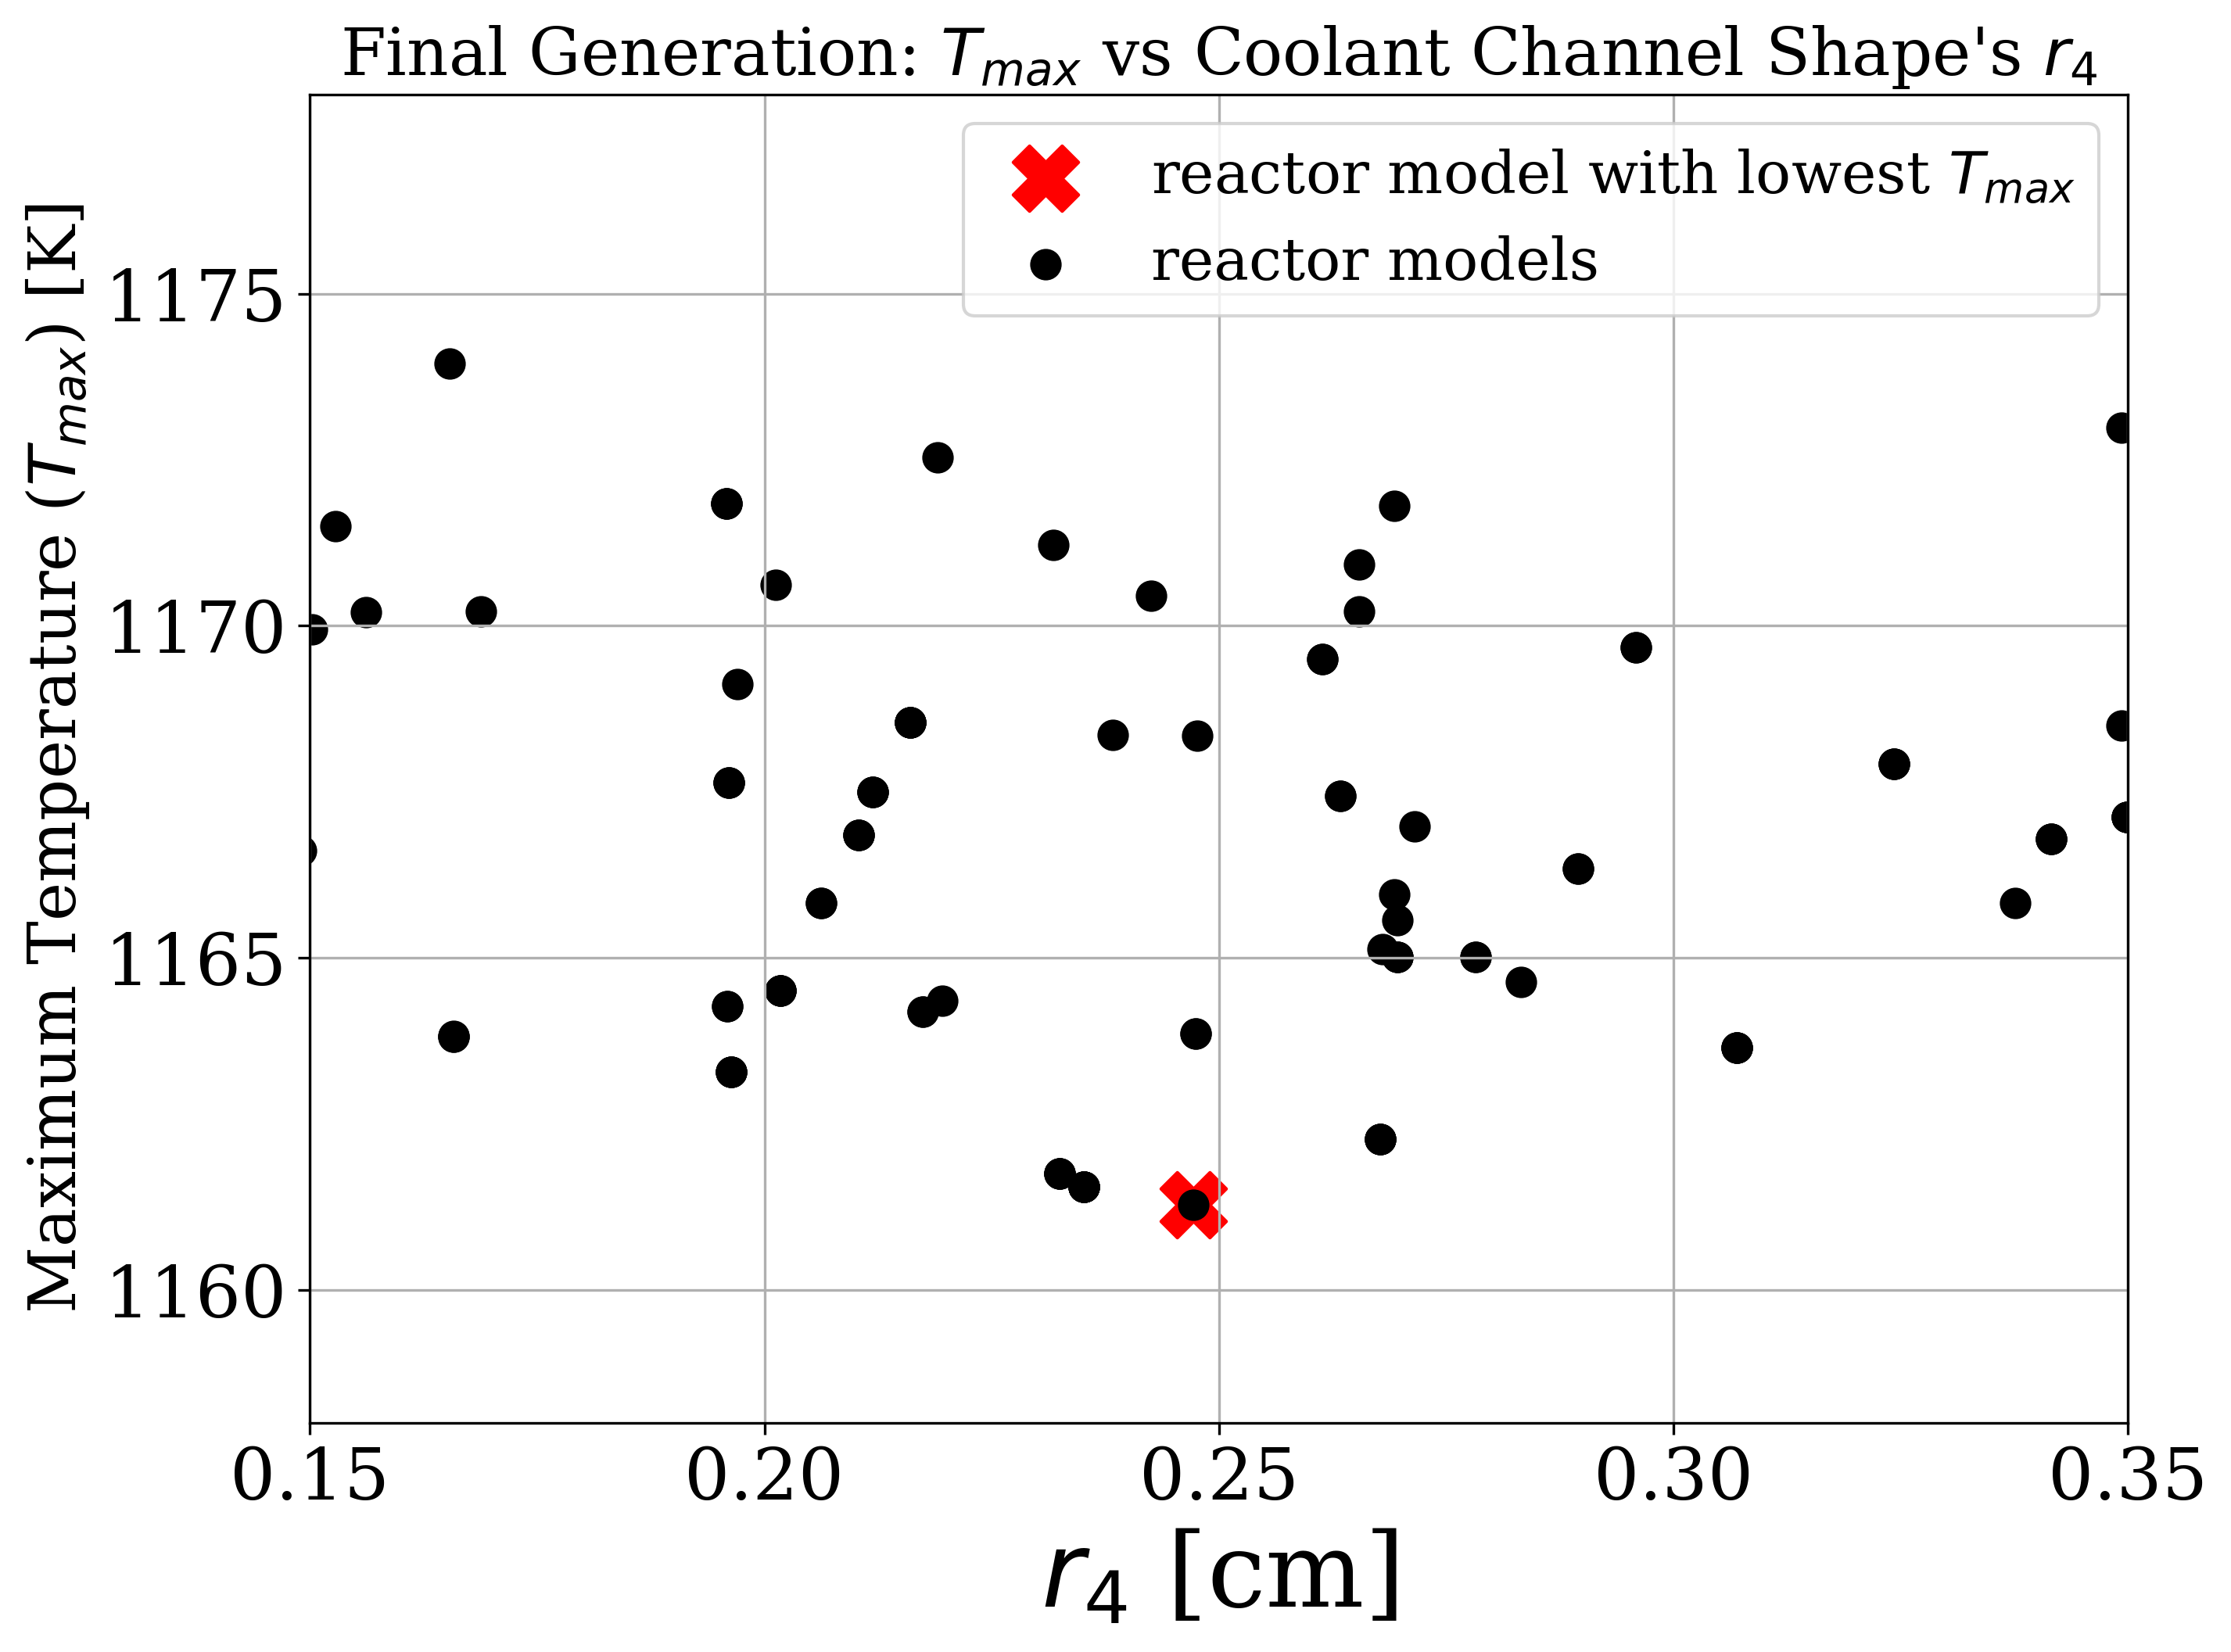
\includegraphics[width=\linewidth]{figures/a-1e-r4-pres.png}}
            \only<3>{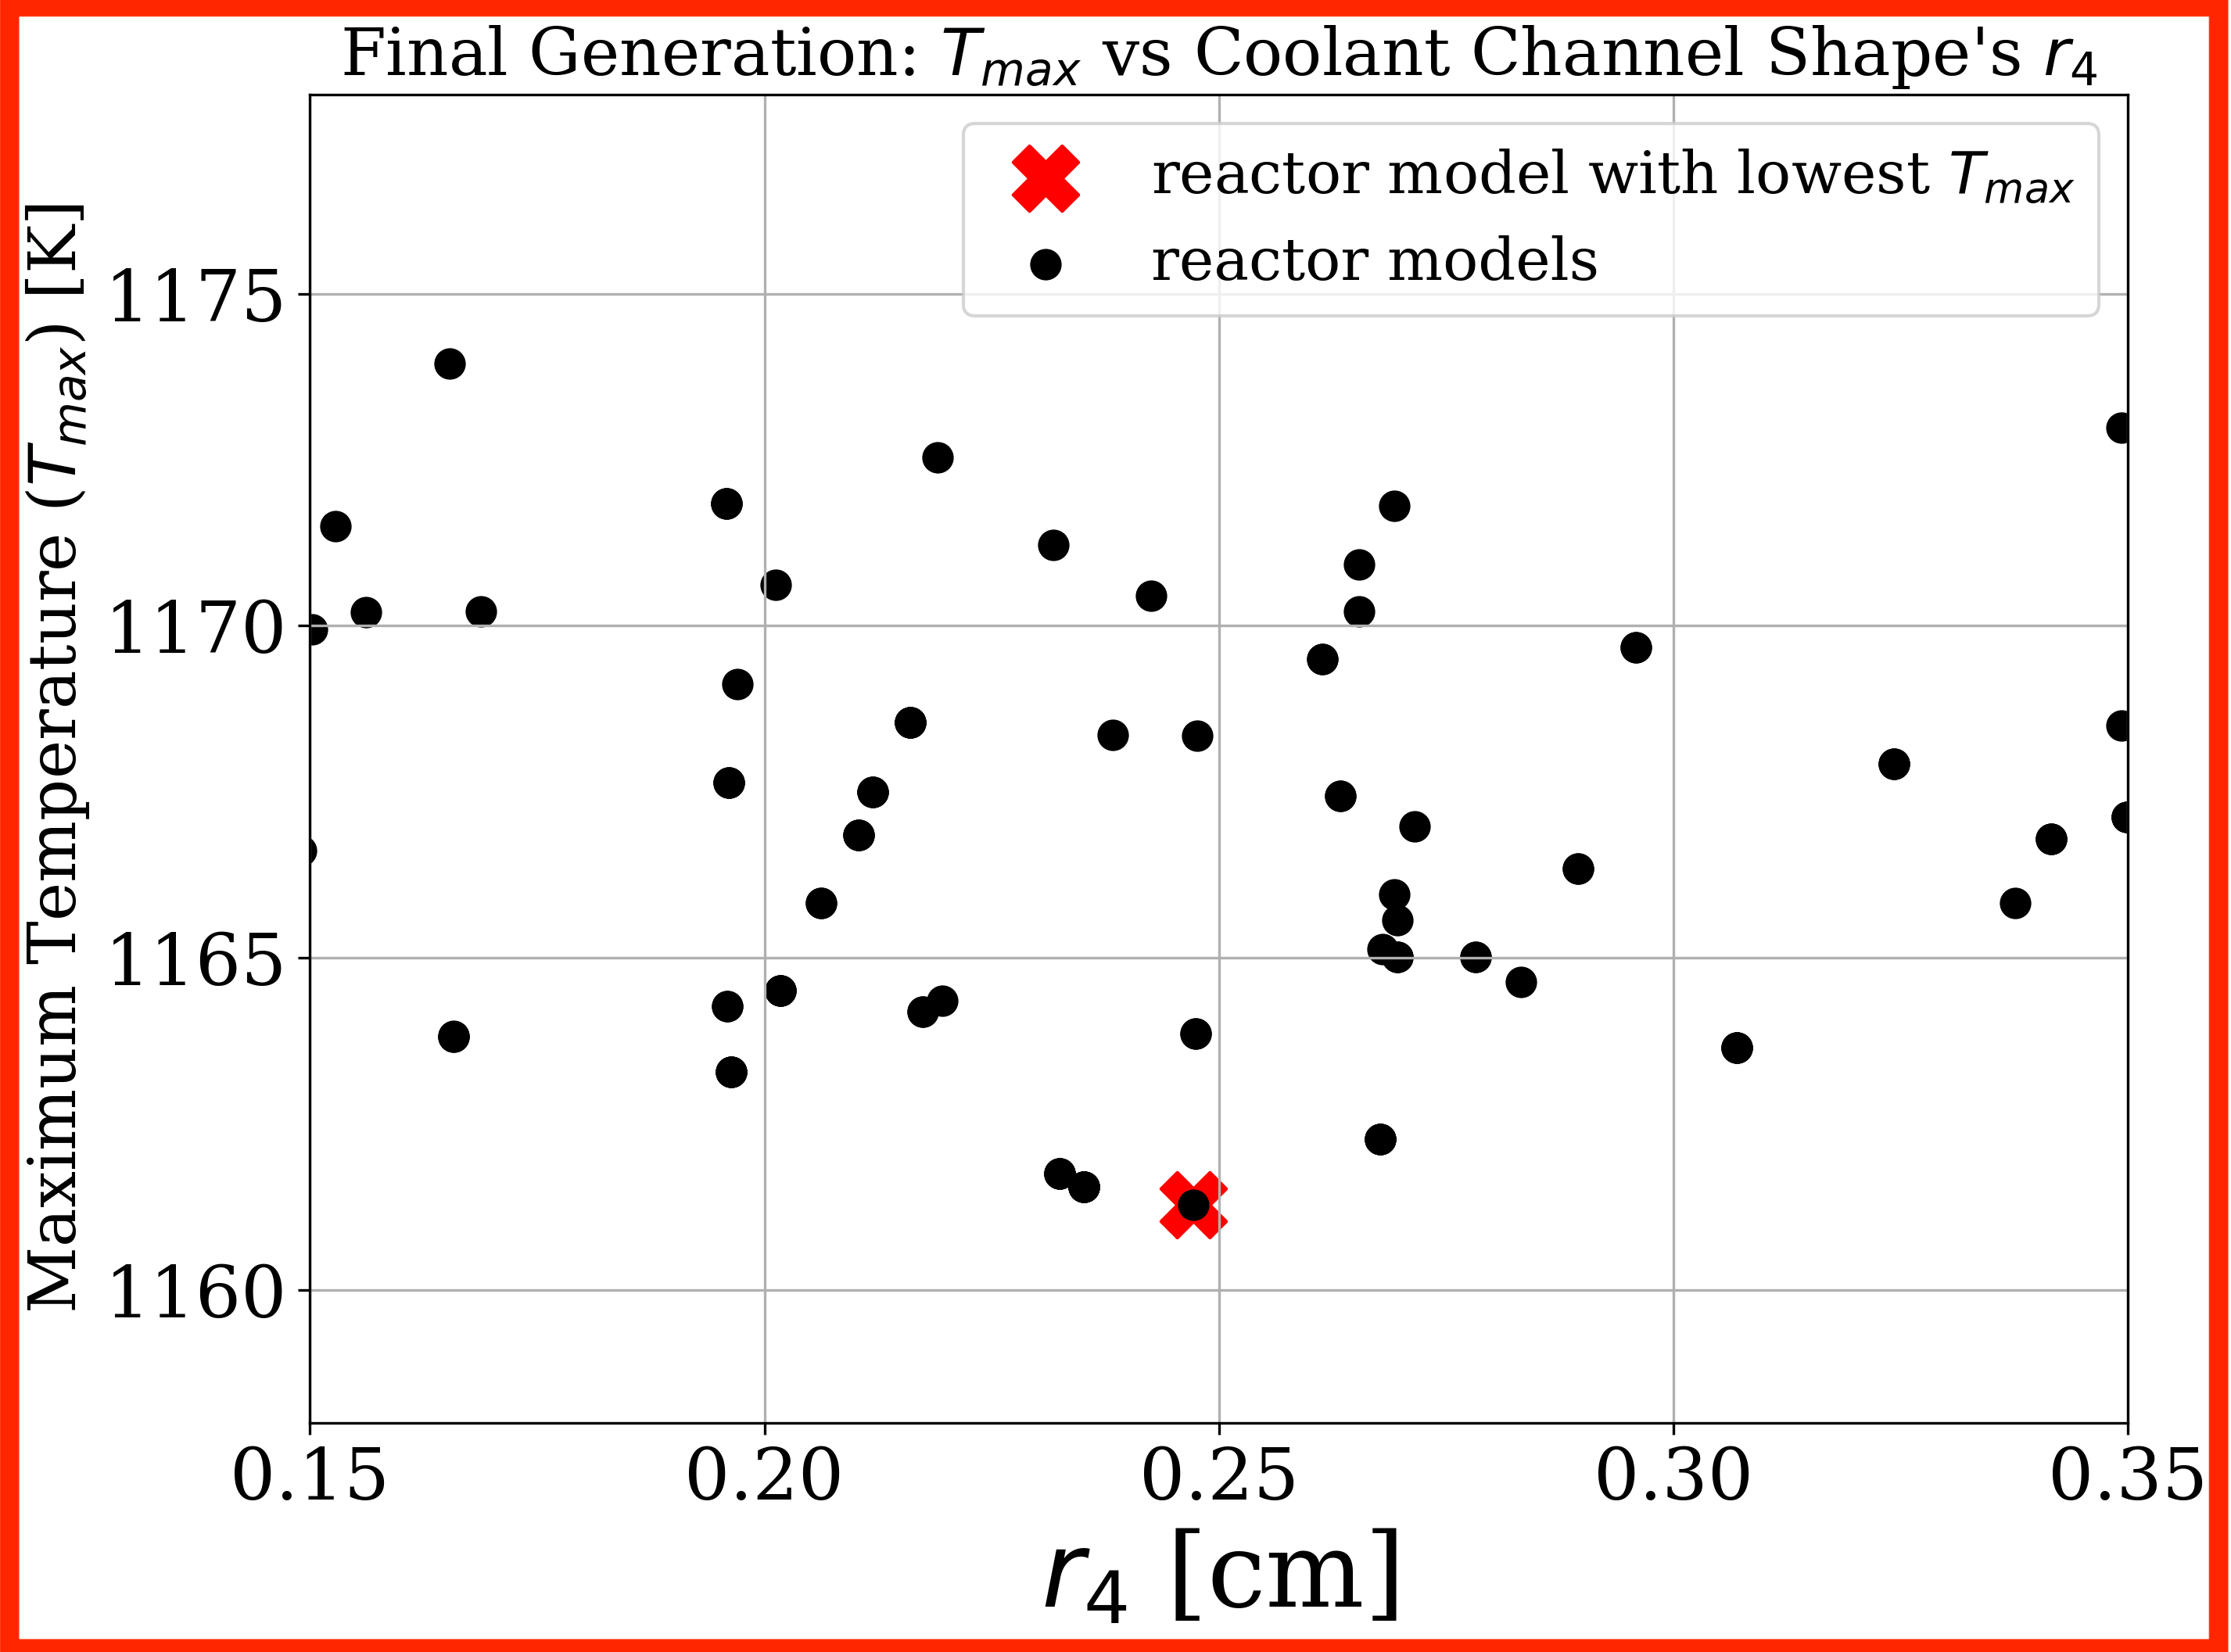
\includegraphics[width=\linewidth]{figures/a-1e-r4-pres-annotated.png}}
            \vspace{-0.5cm}
            \caption{Plot of $T_{max}$ against $r_4$.}
        \end{subfigure}
        \begin{subfigure}{0.3\textwidth}
            \only<1,3>{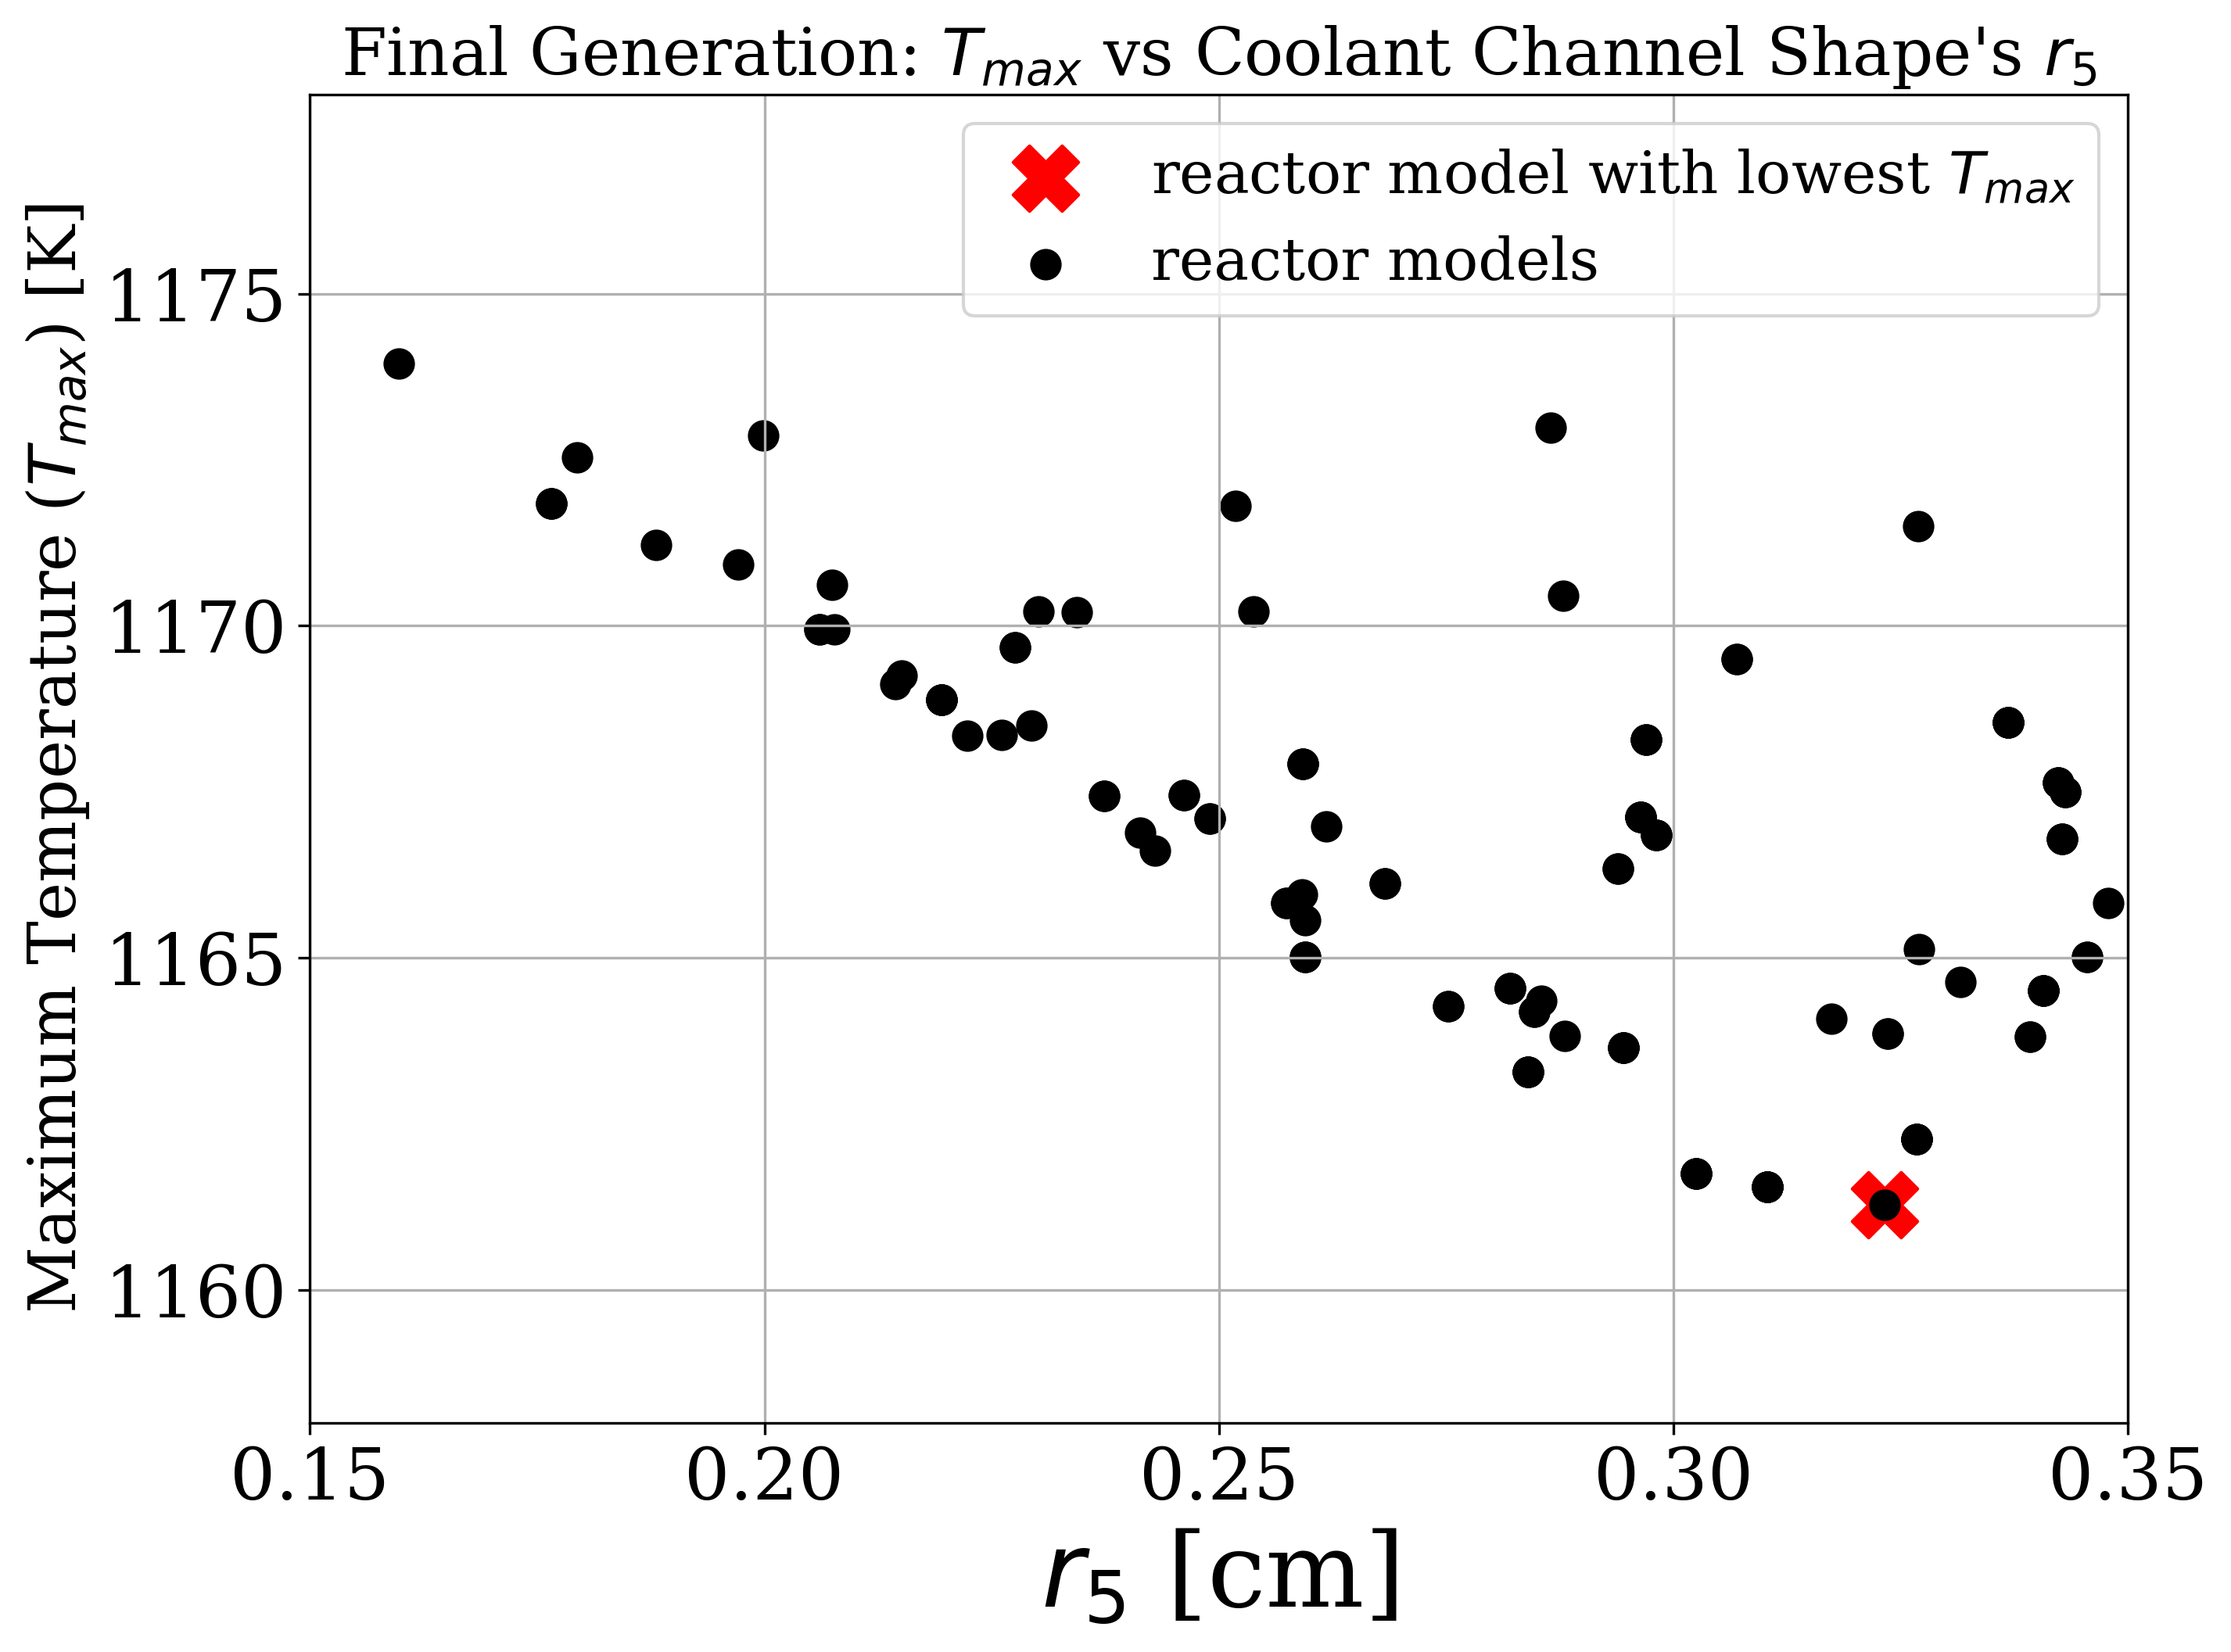
\includegraphics[width=\linewidth]{figures/a-1e-r5-pres.png}}
            \only<2>{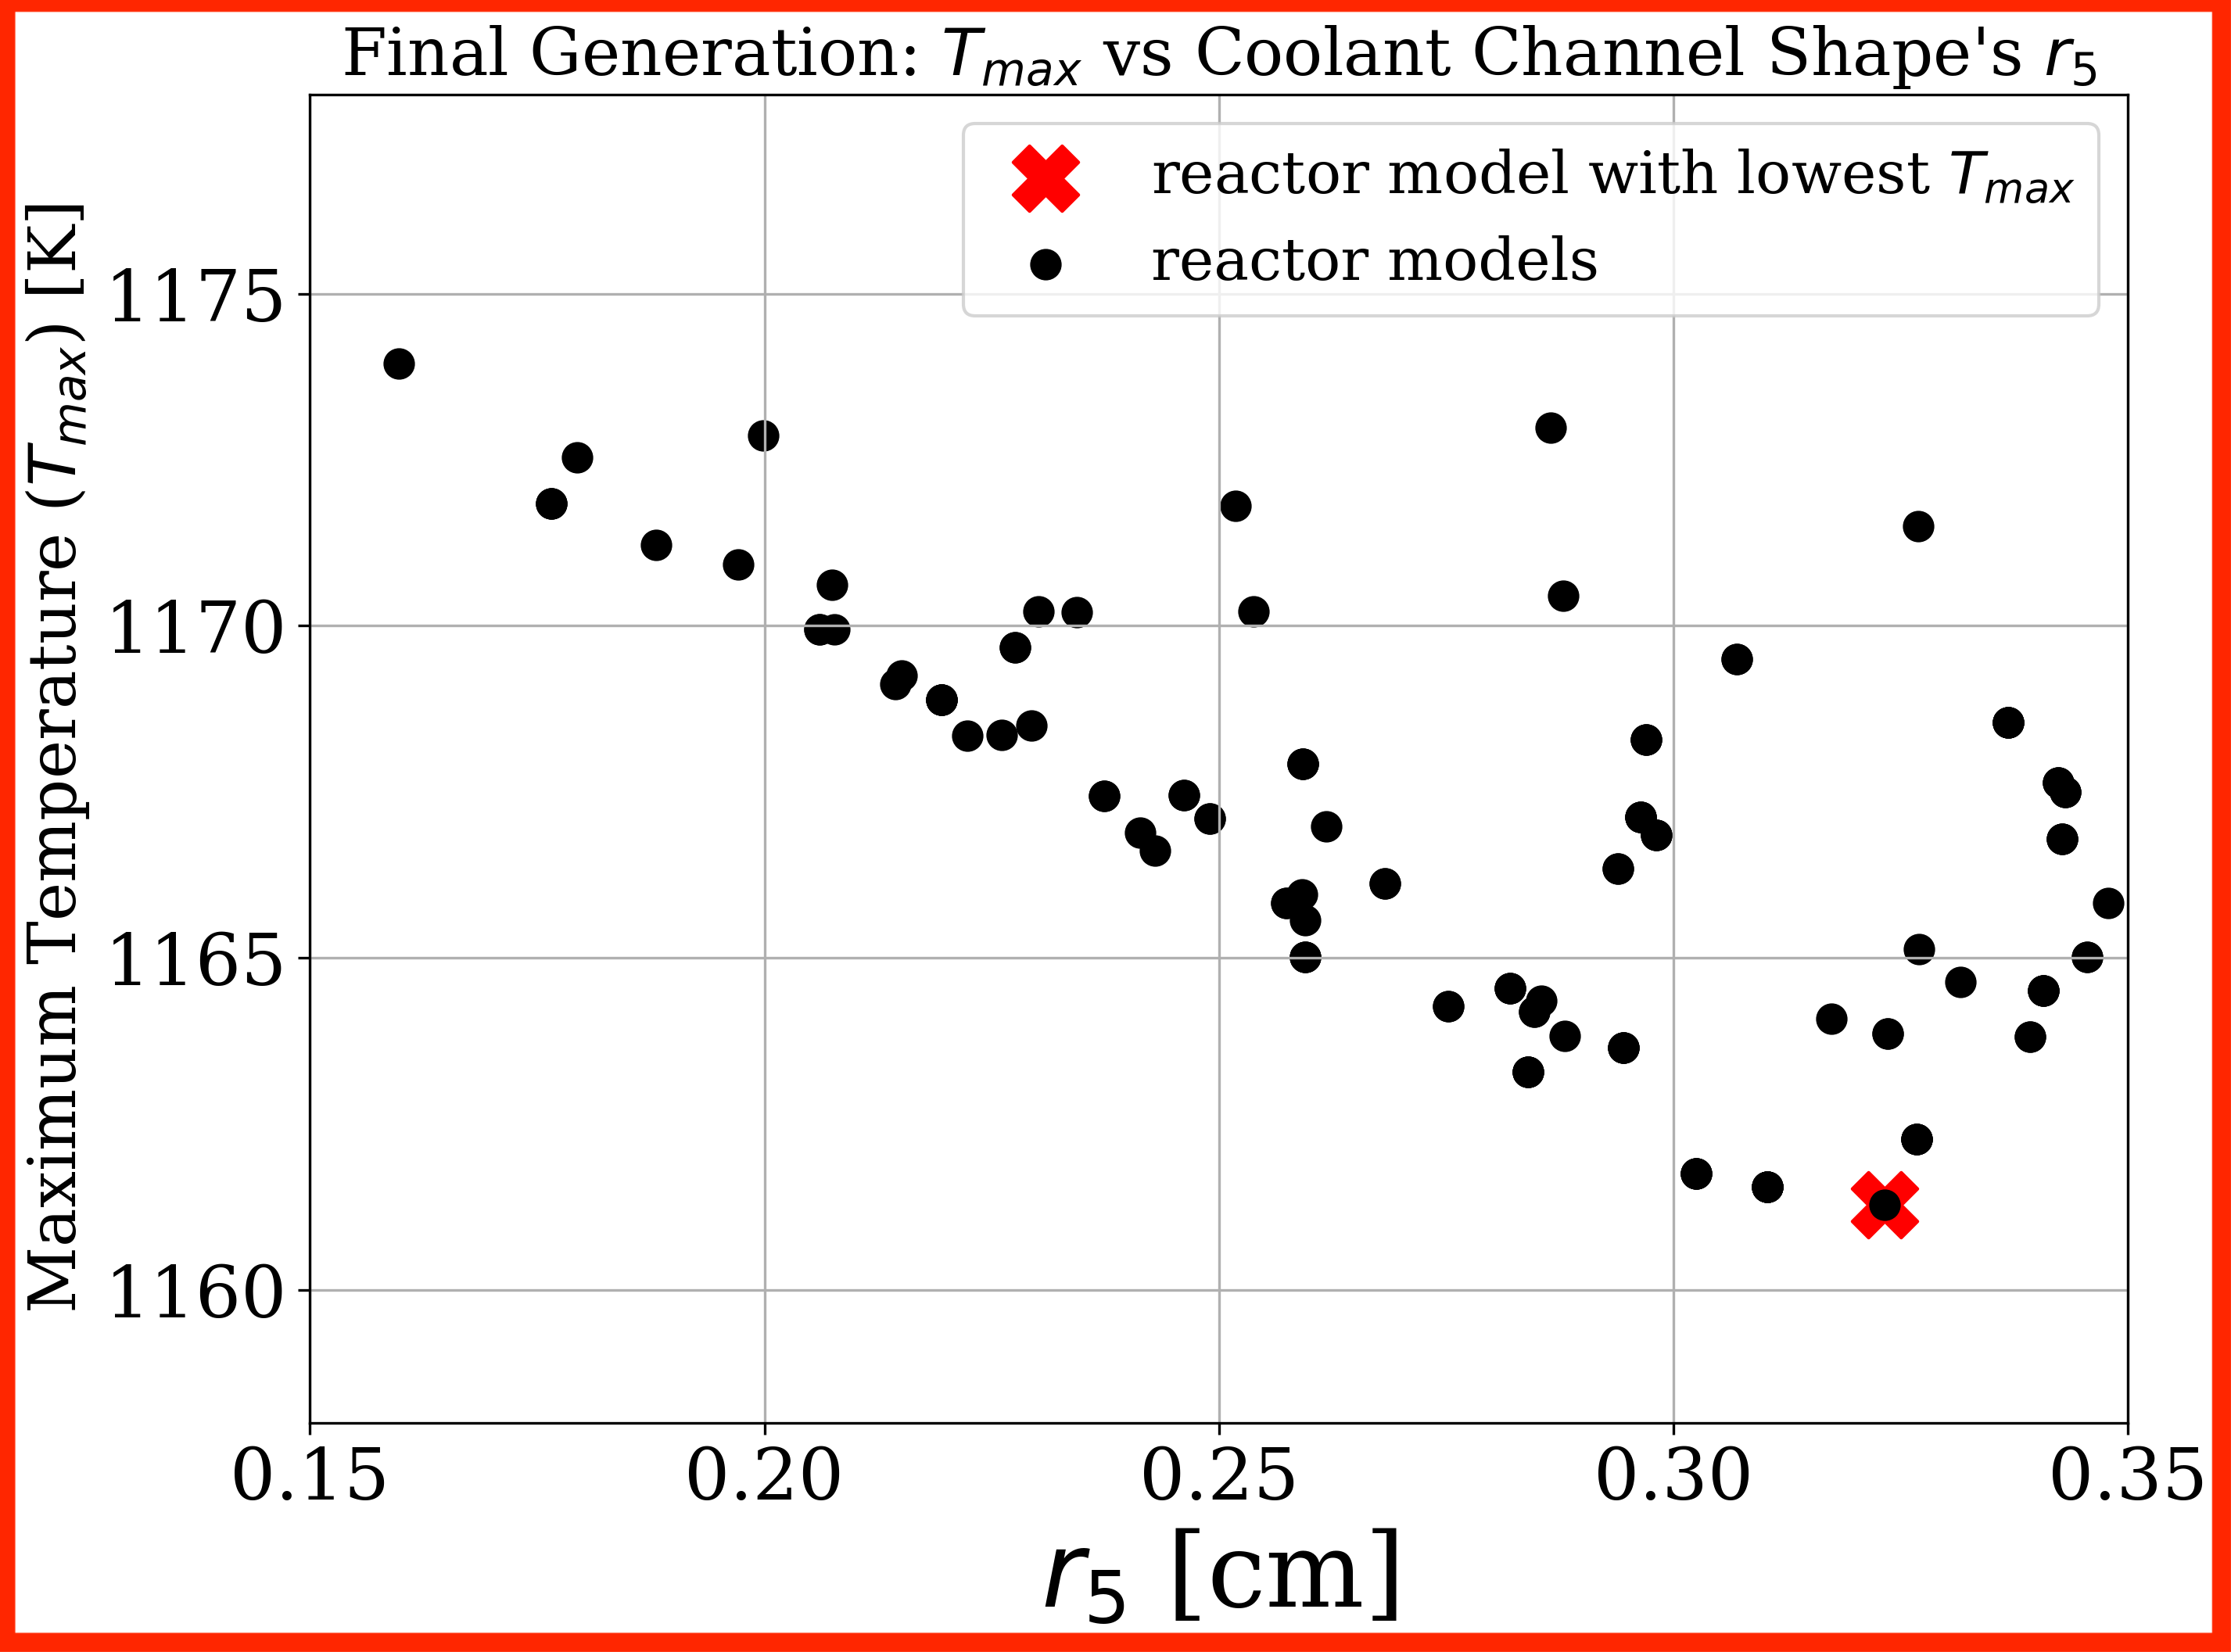
\includegraphics[width=\linewidth]{figures/a-1e-r5-pres-annotated.png}}
            \vspace{-0.5cm}
            \caption{Plot of $T_{max}$ against $r_5$.}
        \end{subfigure}
    \end{figure}
    \only<1>{\textbf{Plots demonstrate if $T_{max}$ is correlated with each radius values.}}
    \only<2>{\textbf{There is a strong negative linear correlation between $T_{max}$ and 
    $r_1$ and $r_5$.}}
    \only<3>{\textbf{Random scattering shows that $T_{max}$ has a weak correlation with 
    $r_2$, $r_3$, $r_4$}.}
\end{frame}

\begin{frame}
    \frametitle{AHTR One-Third Assembly Simulation a-1e Results}
    \begin{figure}
        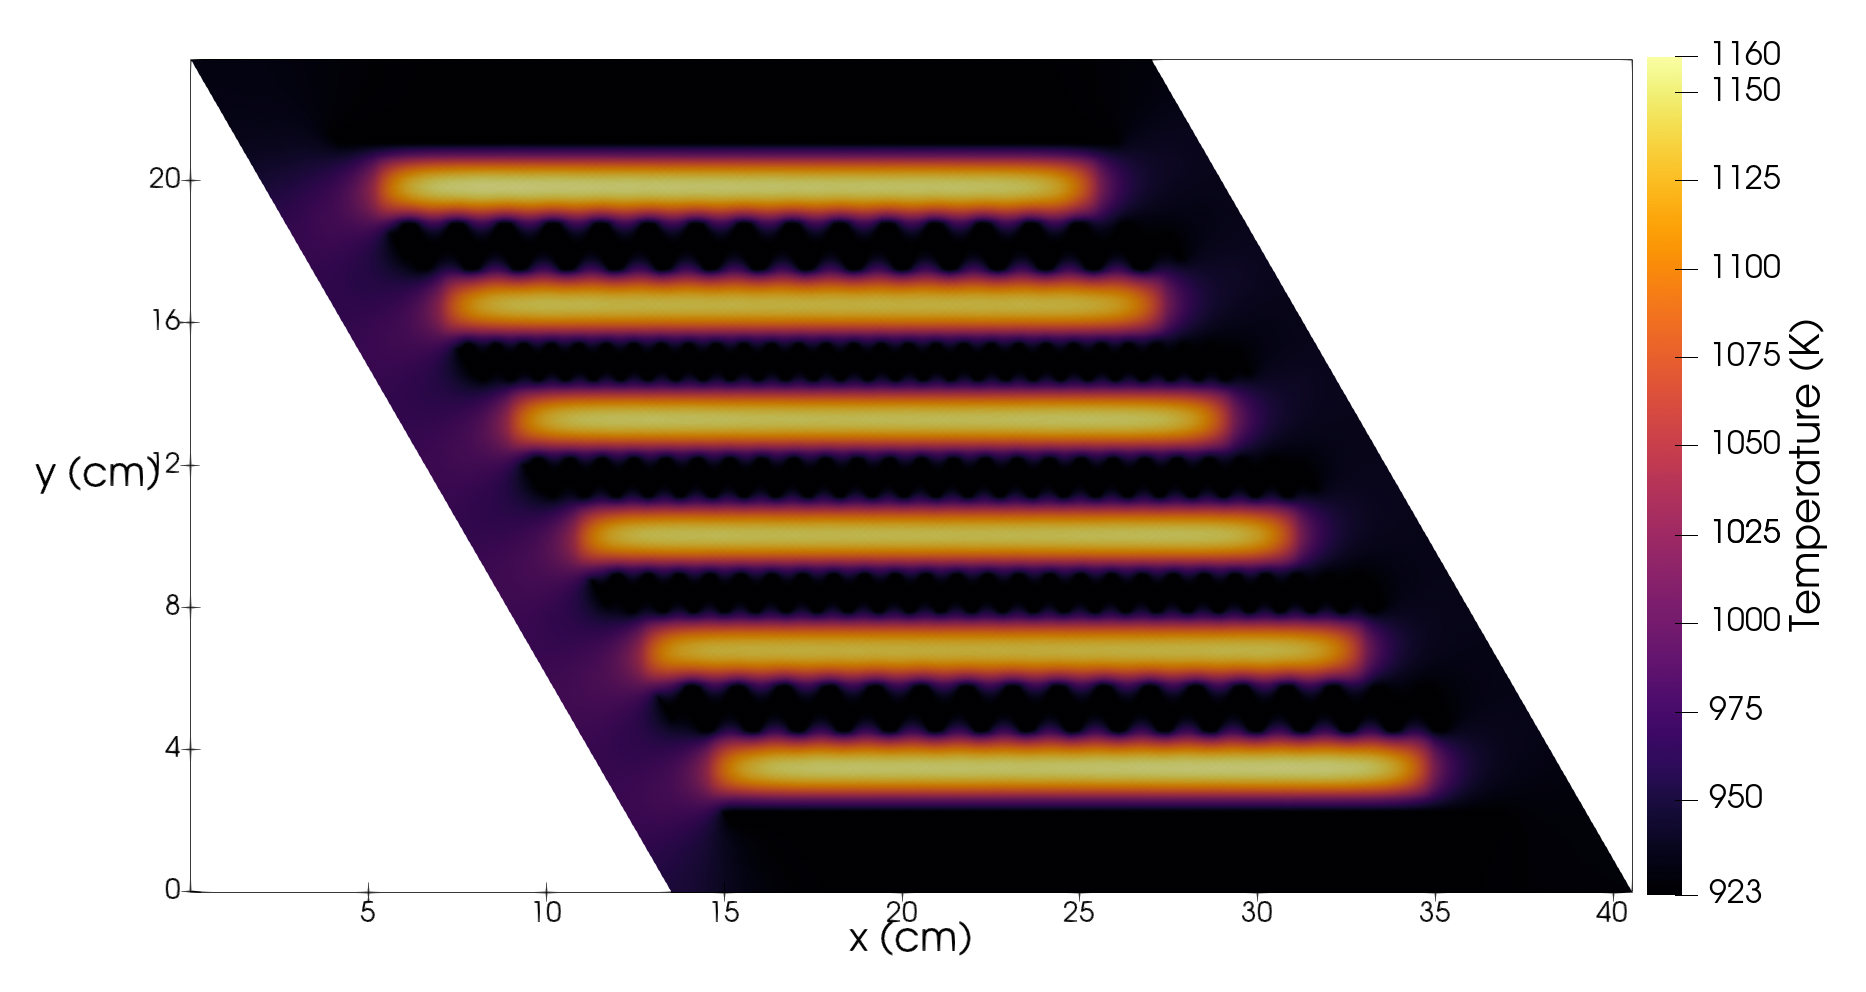
\includegraphics[width=0.59\linewidth]{../docs/figures/a-1e-temp-distribution-2d.png} 
        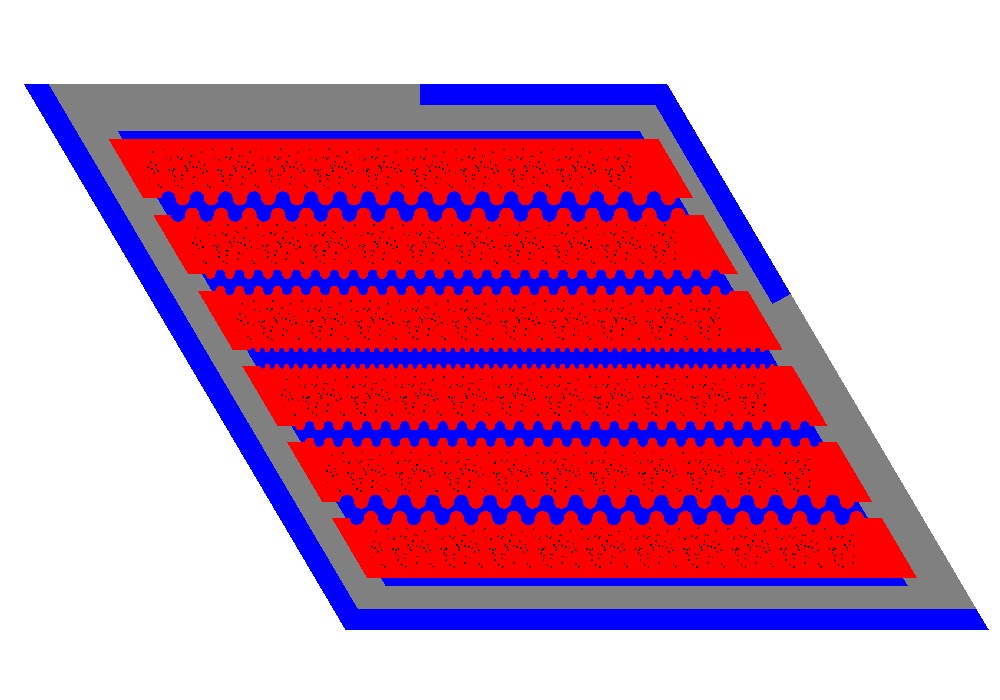
\includegraphics[width=0.4\linewidth]{../docs/figures/coolant-channel-shape-assem.png} 
        \caption{Temperature Distribution in the reactor model with the lowest $T_{max}$.}
    \end{figure}

    To minimize $T_{max}$, ROLLO maximized $r_1$ and $r_5$ to enable enhanced cooling 
    in the top and bottom planks where the temperature peaking was occurring.

    \visible<2->{\begin{tcolorbox}[colback=illiniorange,colframe=illiniorange!50!black]
    \textbf{FLiBe channels located closest to temperature peaks shows a \\ negative 
    correlation with $T_{max}$.}
    \end{tcolorbox}}
\end{frame}

\begin{frame}
    \frametitle{Single-Objective Optimization Major Takeaways}
    \visible<1->{\textbf{Minimize $PF_{total}$ Objective} 
    \begin{itemize}
        \item Driven by maximizing total fission reaction rate
        \item Influences oscillations in TRISO's spatial distribution
        \item No correlation with coolant channel shape  
    \end{itemize}}

    \vspace{0.2cm}
    \visible<2->{\textbf{Minimize $T_{max}$ Objective}
    \begin{itemize}
        \item The minimize $T_{max}$ objective prefers a flatter TRISO distribution 
        \item FLiBe channels located closest to temperature peaks shows a negative 
        correlation with $T_{max}$
    \end{itemize}}

    \vspace{0.2cm}
    \visible<3->{\textbf{Minimize $PPF_{fuel}$ Objective} 
    \begin{itemize}
        \item Driven by flattening thermal flux distribution
        \item Influences oscillations in TRISO's spatial distribution
        \item No correlation with coolant channel shape  
    \end{itemize}}
\end{frame}

\begin{frame}
    \frametitle{AHTR One-Third Assembly Simulation a-2b Results}
    \begin{columns}[t]
        \only<1>{\begin{column}{0.35\textwidth}
        \begin{block}{Simulation a-2b}
        \begin{itemize}
        \item I vary $PF_{total}$ and \textbf{a, b, c, d, e f} 
        ($\rho_{TRISO}(\vec{x}, \vec{y}$)) 
        \item Minimize $PF_{total}$ and $PPF_{fuel}$ objectives
        \item 5 generations 
        \item 128 reactor models per gen  
        \item Total runtime: 492 Theta node-hours
        \end{itemize}
        \end{block}
        \end{column}}
        \only<2>{\begin{column}{0.5\textwidth}
            \begin{block}{Pareto Front}
            \begin{itemize}
                \item Multi objective optimization with competing objectives will return 
                \textbf{multiple optimal solutions that meet each objective to varying 
                degrees}
                \item For each reactor model on the Pareto front, \textbf{none of the 
                objective values can be improved without degrading another}
            \end{itemize}
        \end{block}
        \end{column}}
        \only<3>{\begin{column}{0.35\textwidth}
            \vspace{-0.4cm}
            \begin{block}{Simulation a-2b}
            \begin{itemize}
            \item The 12 reactor models on simulation a-2b's Pareto front have different 
            $PF_{total}$ and $\rho_{TRISO}(\vec{r})$ depending on \textbf{extent each
            objective is minimized.}
            \item Reactor 11 = lowest $PF_{total}$, highest $PPF_{fuel}$
            \item Reactor 3 = lowest $PPF_{fuel}$, highest $PF_{total}$
            \item Reactor 5 = minimizes both objectives equally
            \end{itemize}
            \end{block}
            \end{column}}
    \only<1,3>{    
        \begin{column}{0.65\textwidth}
        \textbf{Simulation a-2b's Pareto front shows the tradeoff between 
        minimize $PF_{total}$ and $PPF_{fuel}$ objectives.}
        \begin{figure}
            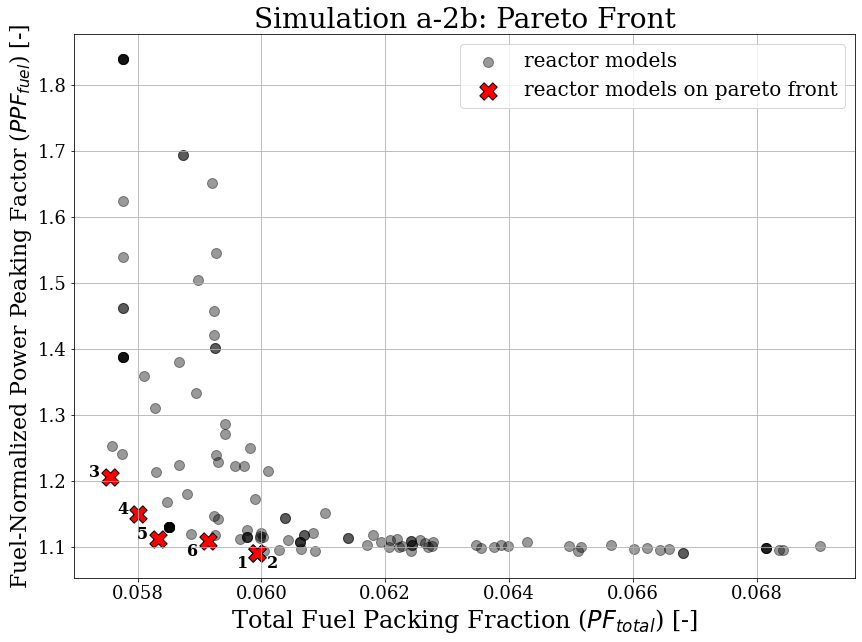
\includegraphics[width=\linewidth]{../docs/figures/assem-obj-2-pfppf-pareto.png} 
        \end{figure}
    \end{column}}
    \only<2>{    
        \begin{column}{0.5\textwidth}
        \begin{figure}
            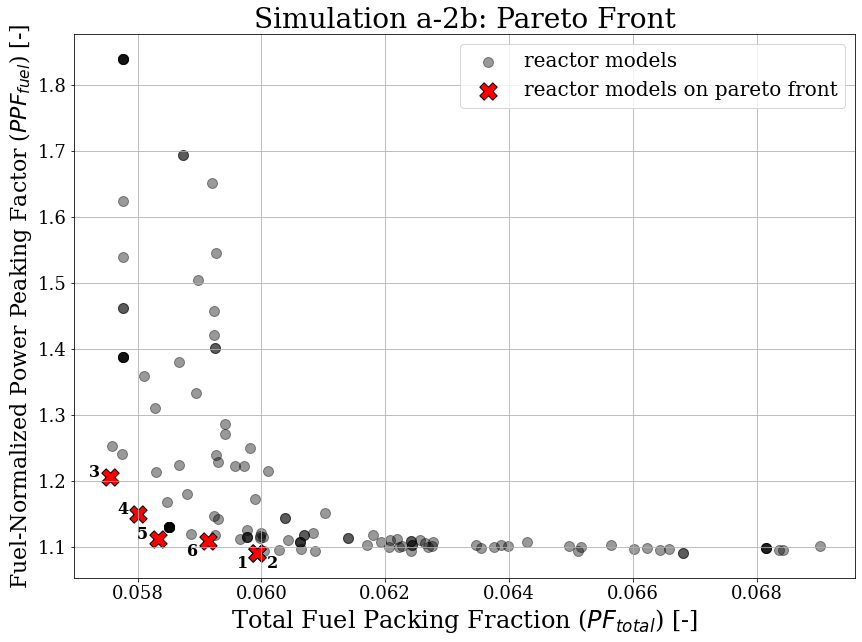
\includegraphics[width=\linewidth]{../docs/figures/assem-obj-2-pfppf-pareto.png} 
        \end{figure}
    \end{column}}
    \end{columns}

    \vspace{0.4cm}
    \only<2>{\textbf{Successful multi-objective optimization finds a wide spread of 
    reactor models on their Pareto fronts}}
\end{frame}

\begin{frame}
    \frametitle{AHTR One-Third Assembly Simulation a-2b Results}
    \centering
    \textbf{ROLLO found a wide variety of TRISO distributions on the Pareto front 
    that minimize each objective to a different extent.}

    \vspace{0.2cm}
    \begin{figure}
        \only<1>{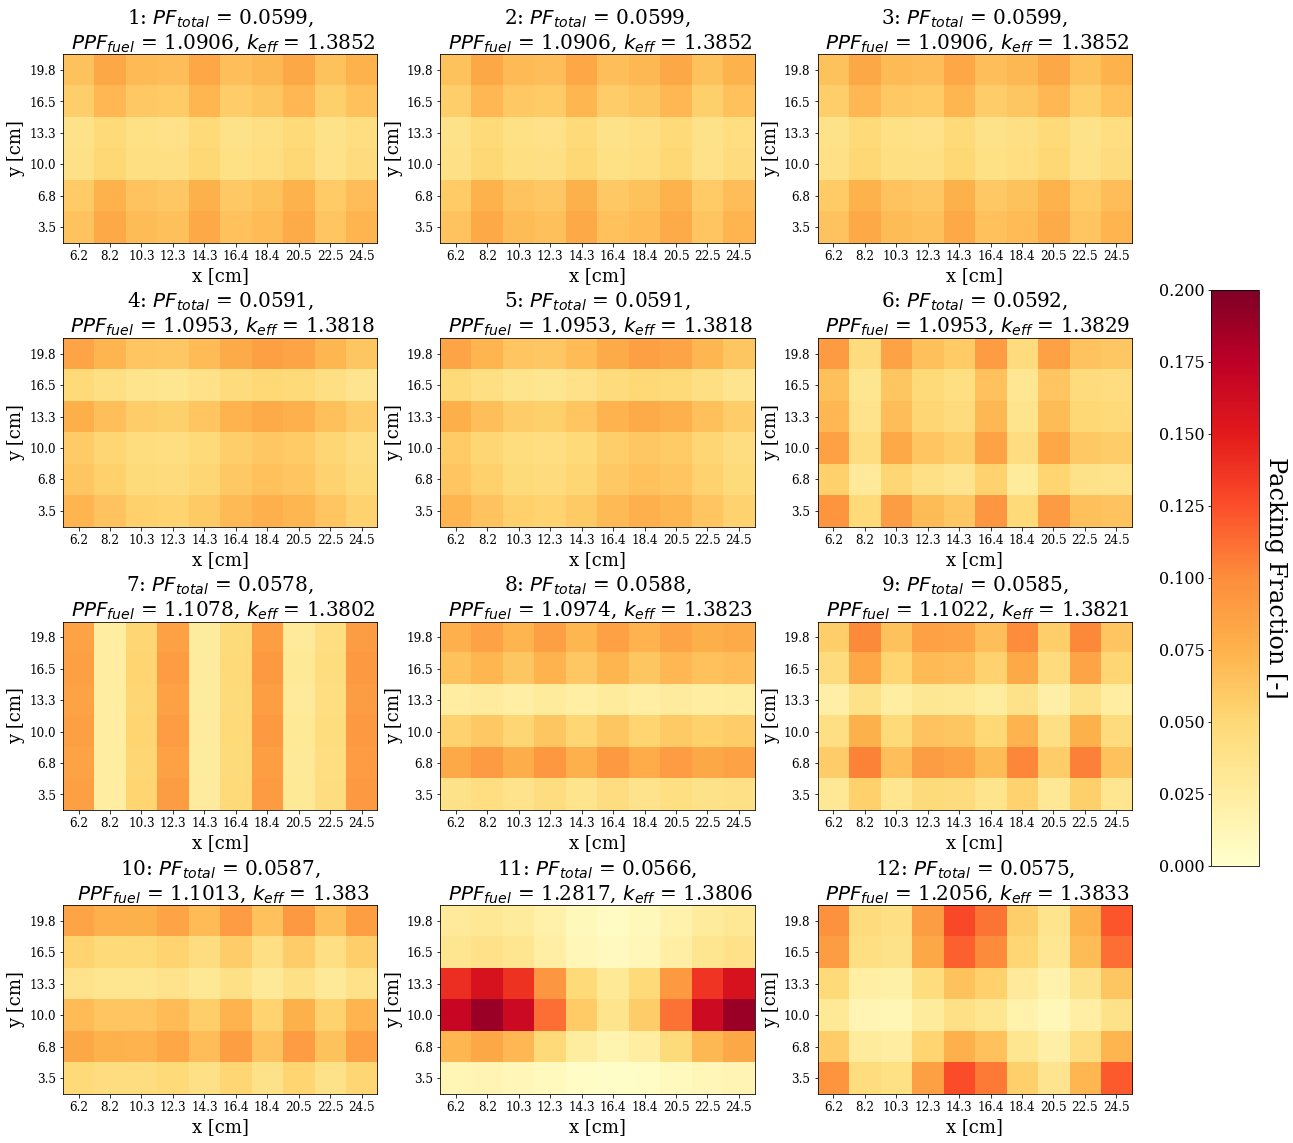
\includegraphics[width=0.8\linewidth]{../docs/figures/assem-obj-2-pfppf-pareto-distr.png}}
        \only<2>{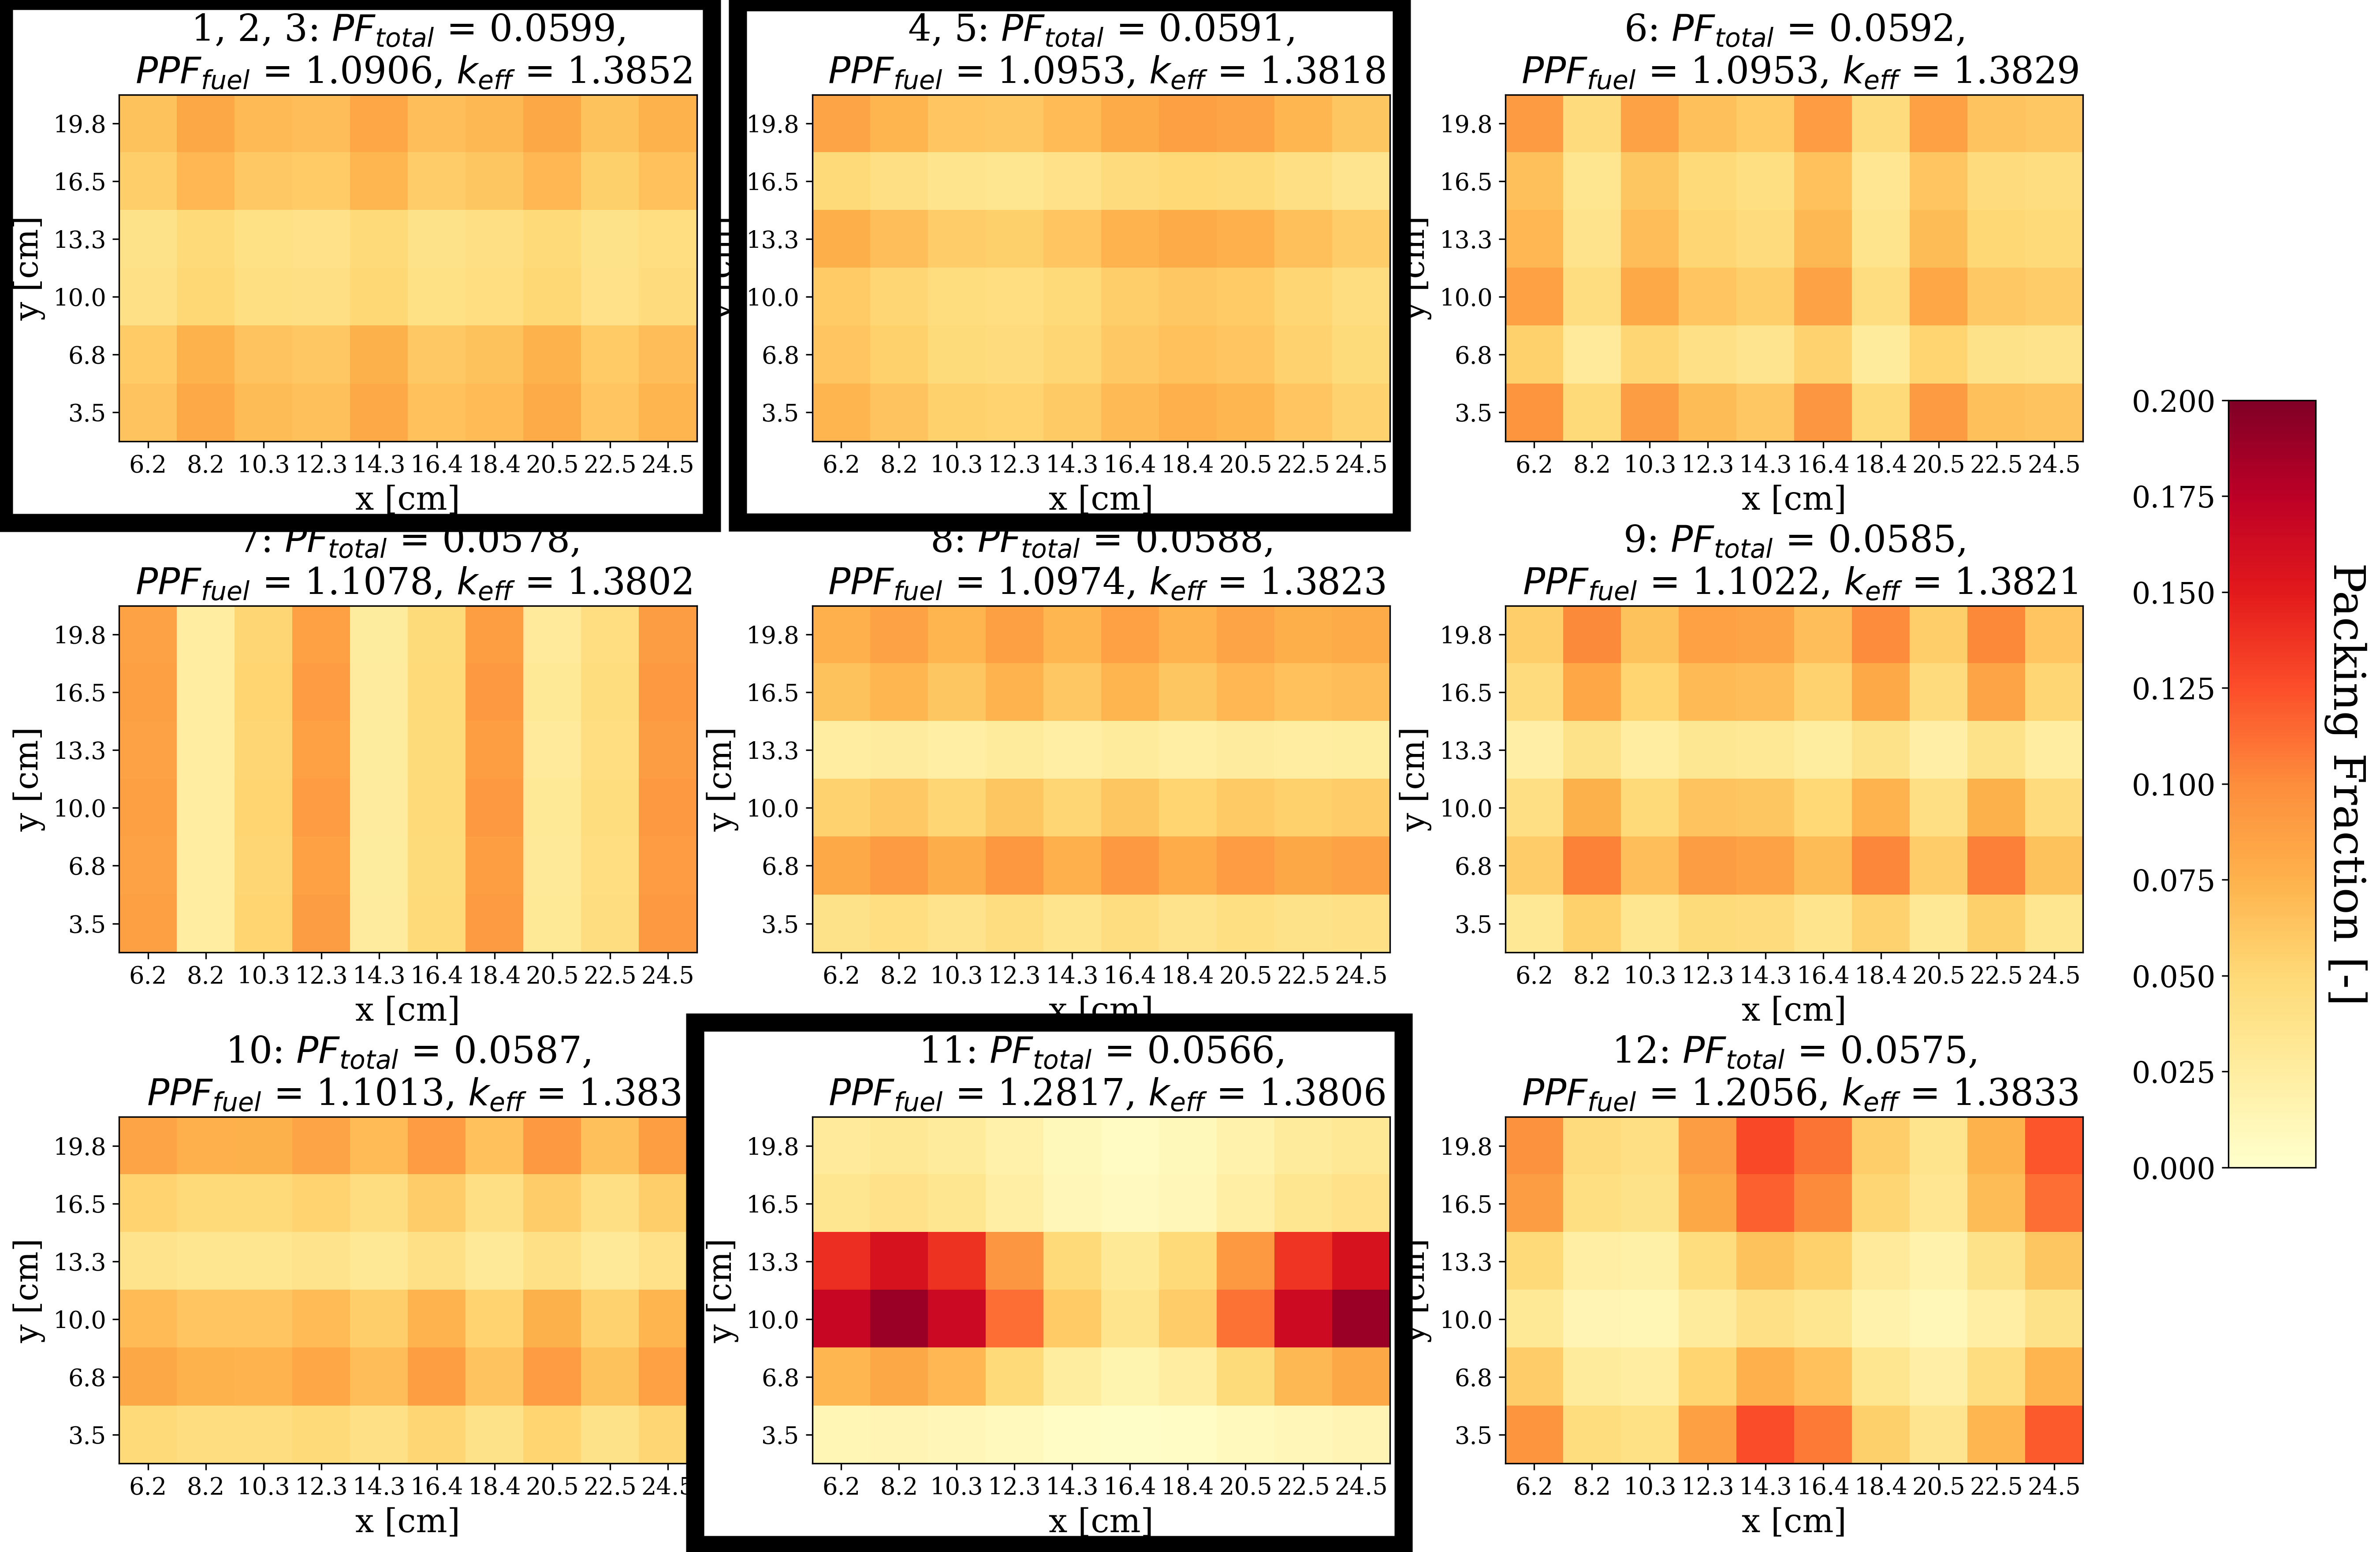
\includegraphics[width=0.8\linewidth]{figures/assem-obj-2-pfppf-pareto-distr-annotated.png}}
    \end{figure}
\end{frame}

\begin{frame}
    \frametitle{AHTR One-Third Assembly Simulation a-2b Results}
    \begin{figure}
        \centering
        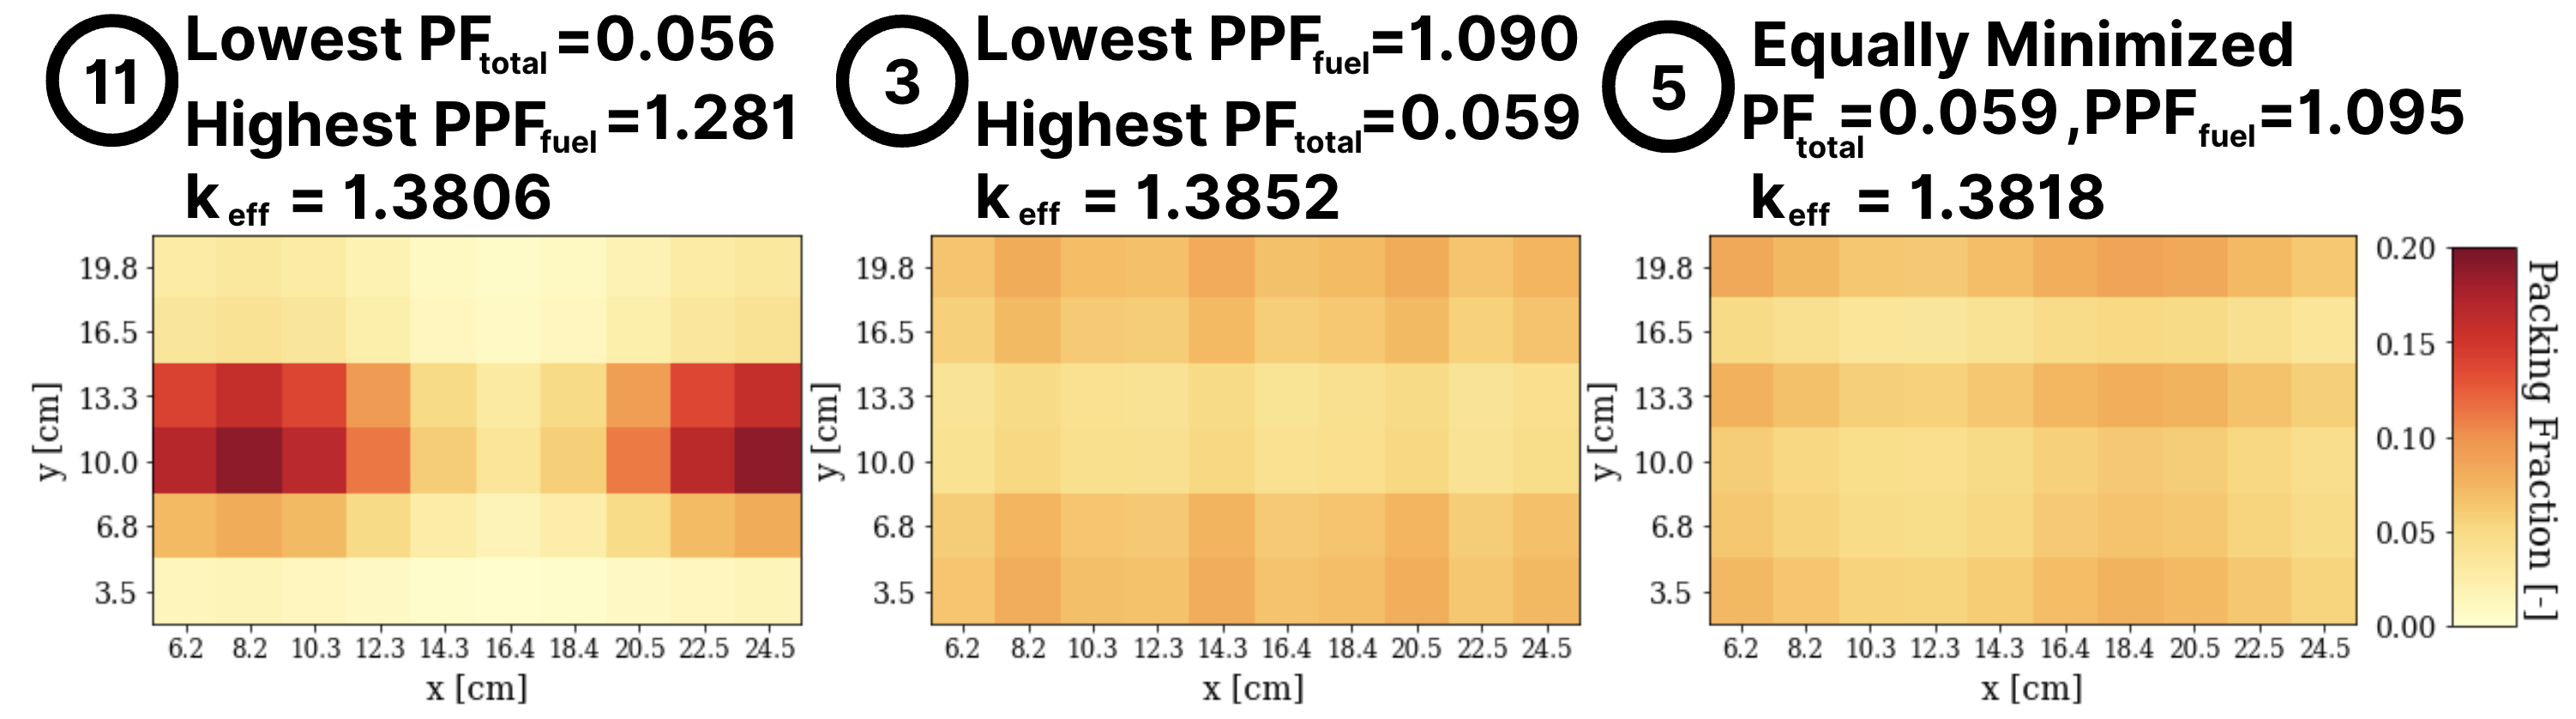
\includegraphics[width=\linewidth]{figures/a-2b-comparison-reactors.png}
    \end{figure}

    Minimize $PF_{total}$ is driven by \textbf{maximizing total fission reaction rate} 
    \begin{itemize}
        \visible<1->{\item Reactor 11 with $PF_{total} = 0.056$ and reactor model 5 with 
        $PF_{total} = 0.059$ have the similar $k_{eff}$ and total fission reaction rate} 
        \visible<2->{\item Reactor 11 TRISO distribution enables it to achieve the 
        same $k_{eff}$ as reactor 5 despite having a lower $PF_{total}$}
        \visible<3->{\item \textbf{Reactor 11 TRISO distribution minimizes spatial 
        self-shielding effects}}
    \end{itemize}
\end{frame}

\begin{frame}
    \frametitle{AHTR One-Third Assembly Simulation a-2b Results}
    \begin{figure}
        \centering
        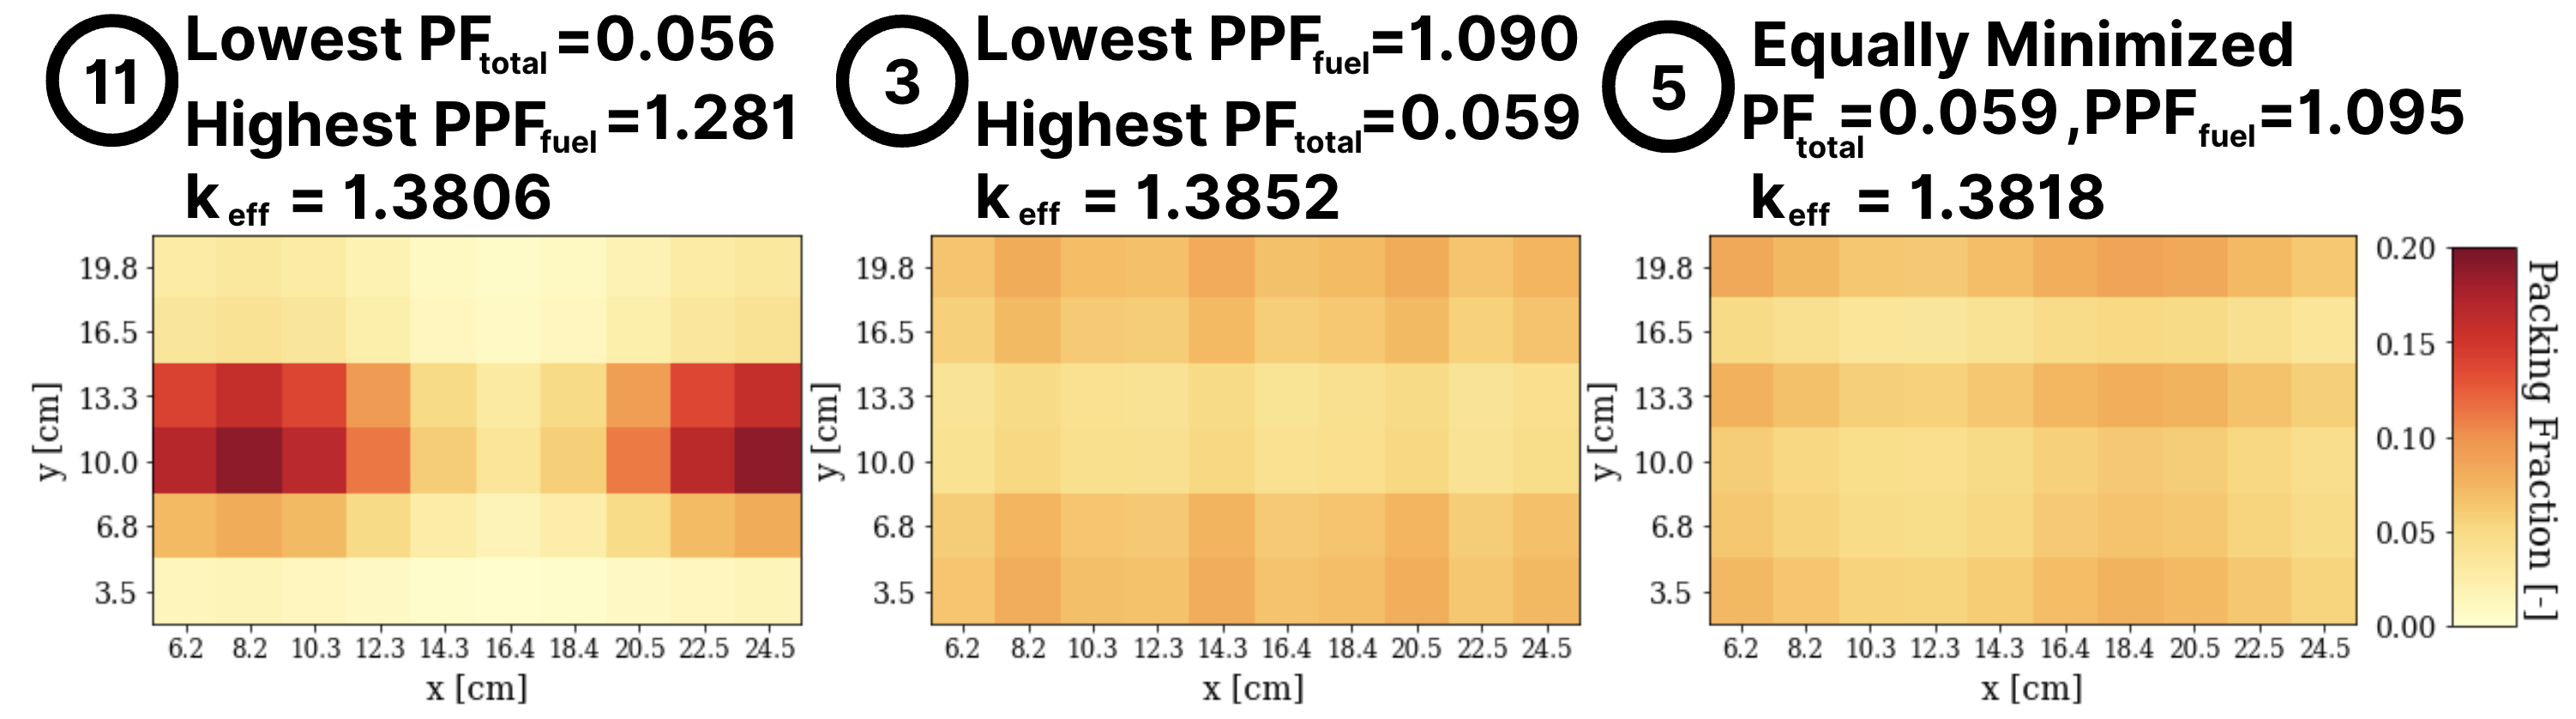
\includegraphics[width=\linewidth]{figures/a-2b-comparison-reactors.png}
    \end{figure}

    Minimize $PPF_{fuel}$ objective is driven by \textbf{flattening thermal 
    flux distribution}  
    \begin{itemize}
        \item Flattest to least flat thermal flux: reactor model 
                $3 \rightarrow 5 \rightarrow 11$
        \item \textbf{Reactor model 3 with lowest $PPF_{fuel}$ has flattest flux}
    \end{itemize}

    \visible<2->{\begin{tcolorbox}[colback=illiniorange,colframe=illiniorange!50!black]
        Minimize $PF_{total}$ and Minimize $PPF_{fuel}$ objectives 
        influence each other resulting in \textbf{unexpected TRISO distributions at 
        different $PF_{total}$ values}. 
    \end{tcolorbox}}
\end{frame}

\begin{frame}
    \frametitle{AHTR One-Third Assembly Simulation a-3b Results}
    \begin{columns}[t]
    \only<1>{\begin{column}{0.35\textwidth}
        \begin{block}{Simulation a-3b}
            \begin{itemize}
            \item Vary $PF_{total}$, \textbf{a, b, c, d, e f} ($\rho_{TRISO}(\vec{x}, 
            \vec{y}$)), and $r_1, r_2, r_3, r_4, r_5$ (coolant channel shape) 
            \item Minimize all three objectives: $PF_{total}$, $T_{max}$ and $PPF_{fuel}$.
            \item 6 generations 
            \item 128 reactor models per gen 
            \item Total runtime: 1528 Theta node-hours 
            \end{itemize}
            \end{block}
        \end{column}}
    \only<2>{\begin{column}{0.4\textwidth}
        \begin{block}{Simulation a-3b}
        \begin{itemize}
        \item The 12 reactor models on simulation a-3b's Pareto front have different 
        input parameters depending on \textbf{extent each
        objective is minimized}
        \item Reactor 11 = lowest $PF_{total}$
        \item Reactor 1 = lowest $T_{max}$
        \item Reactor 4 = lowest $PPF_{fuel}$
        \item Reactor 2 = minimizes all objectives equally
        \end{itemize}
        \end{block}
        \end{column}}

    \begin{column}{0.7\textwidth}
        \only<1>{\textbf{ROLLO successfully found 12 widely spread out reactor models on a-3b's 
        Pareto front.}}
    \begin{figure}
        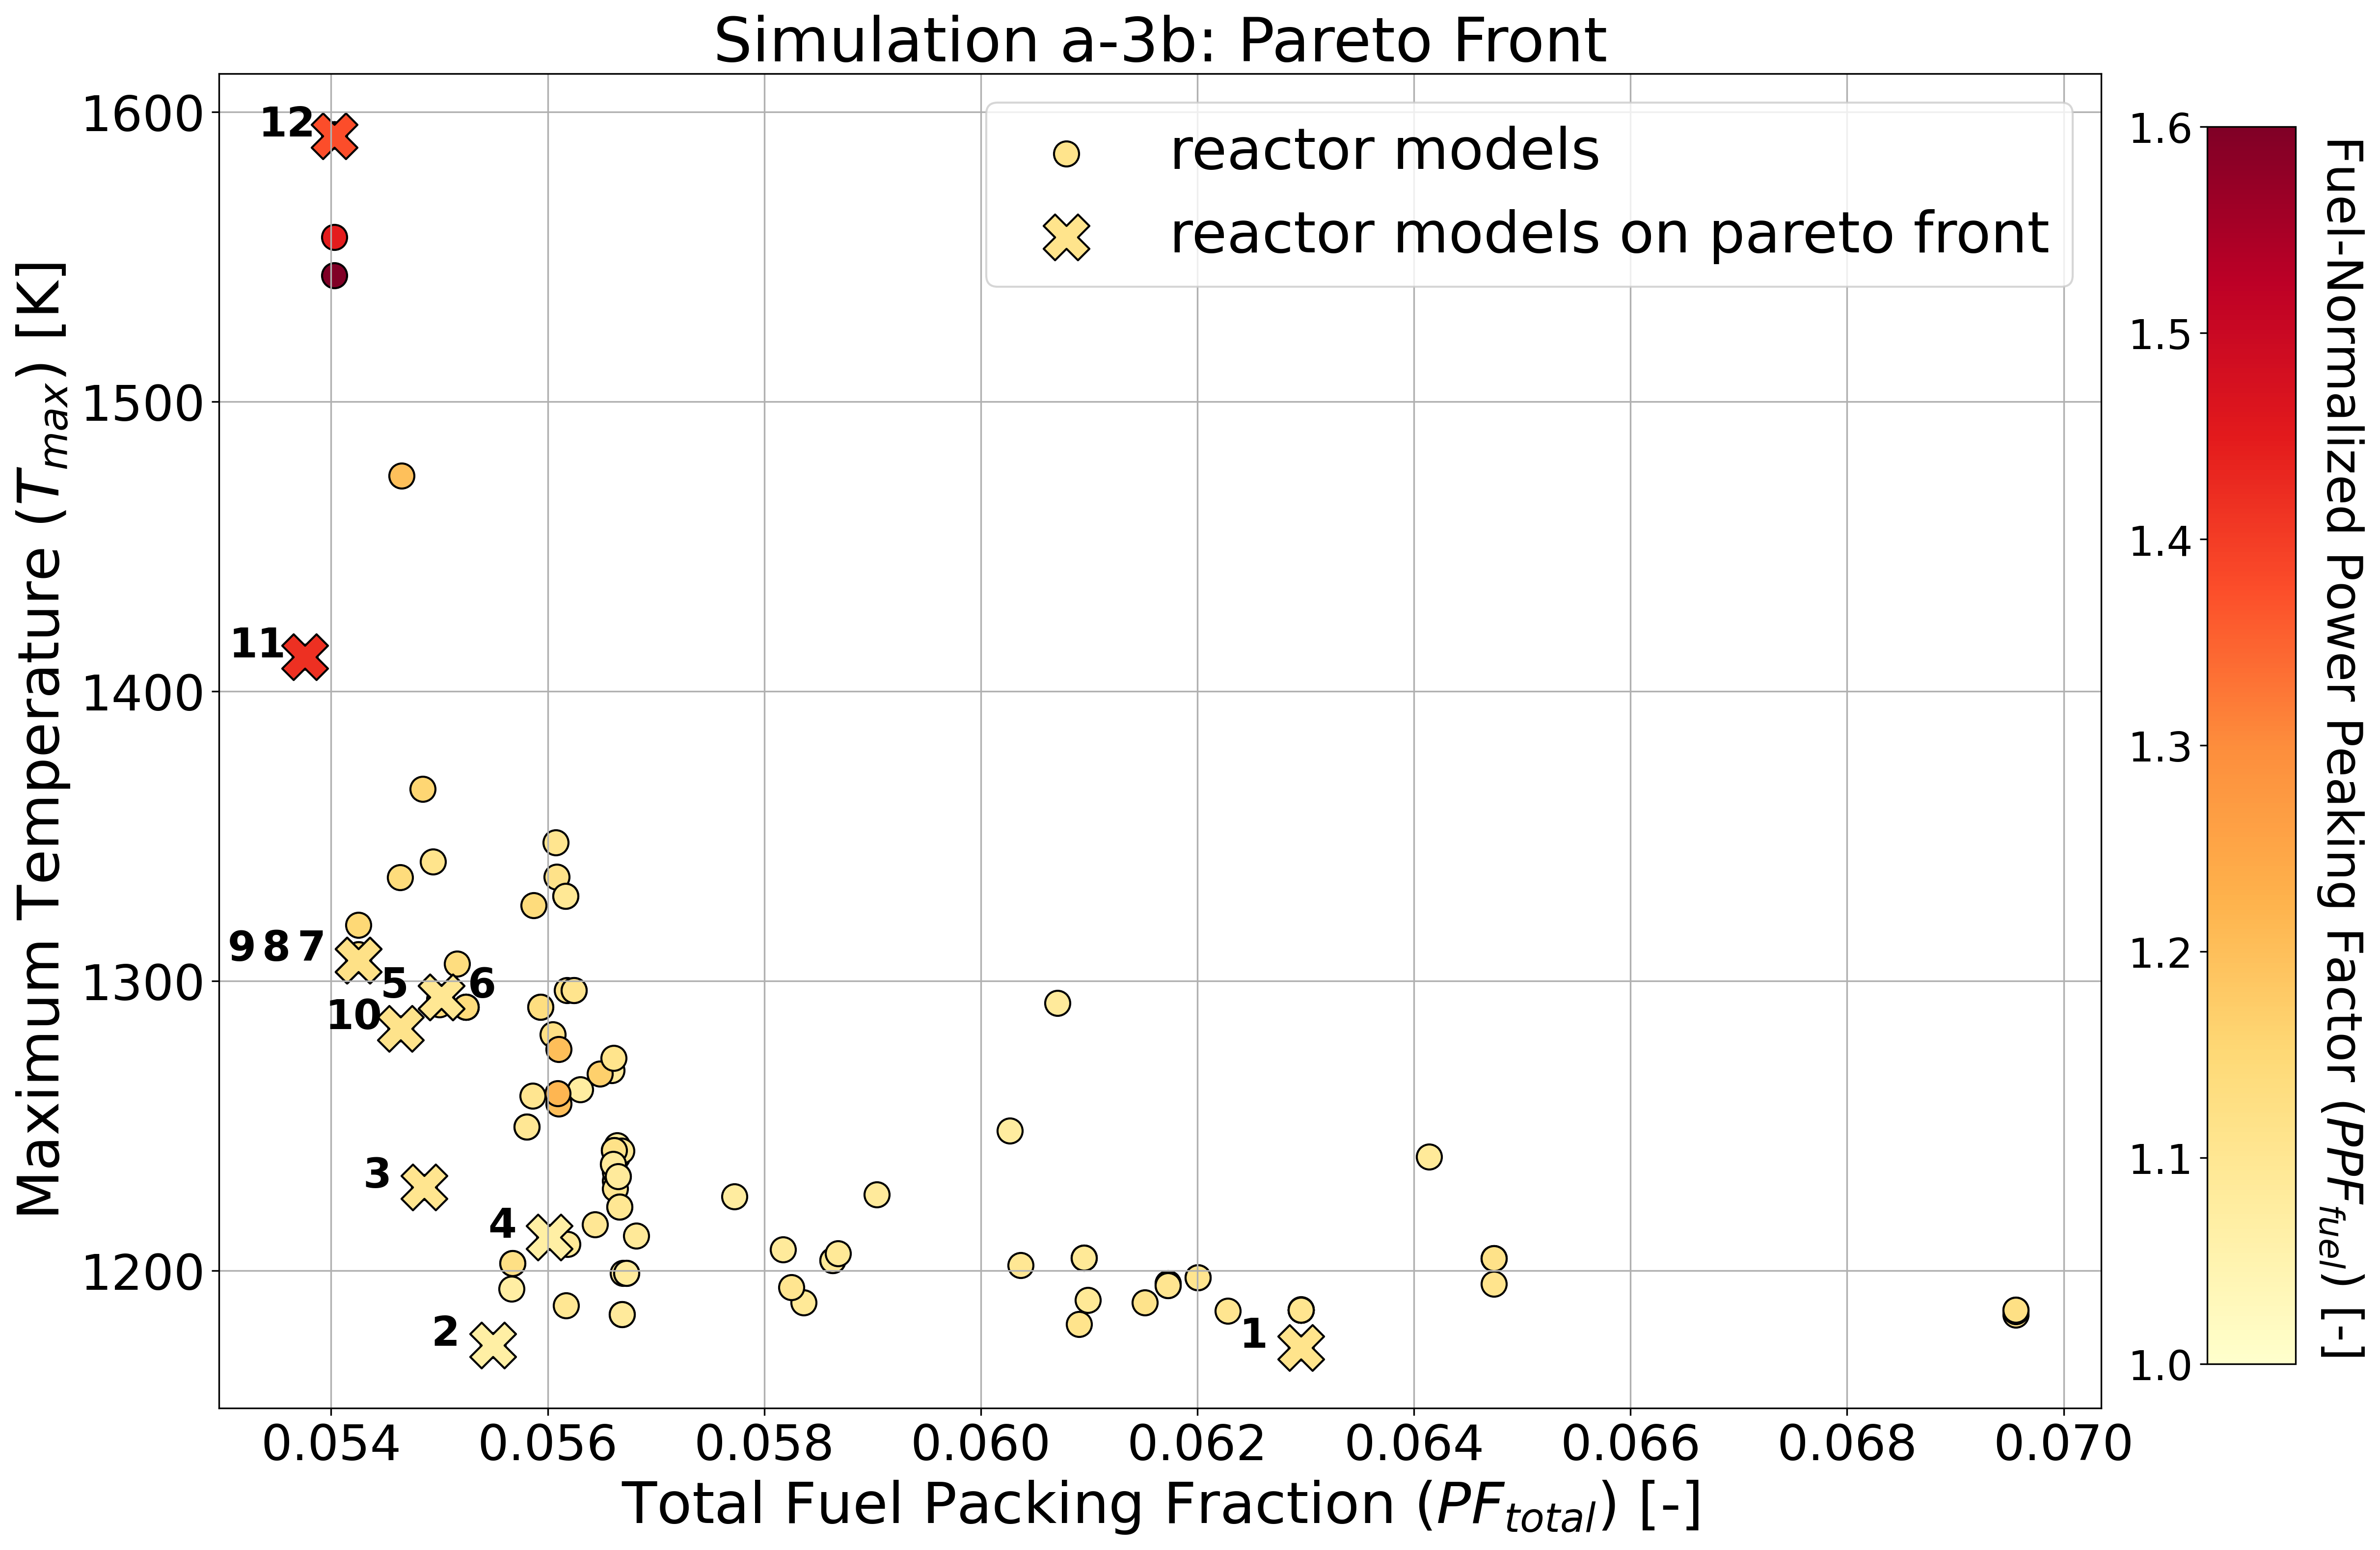
\includegraphics[width=\linewidth]{../docs/figures/assem-obj-3-all-2d.png} 
    \end{figure}
    \end{column}
\end{columns}
\end{frame}

\begin{frame}
    \frametitle{AHTR One-Third Assembly Simulation a-3b Results}
    \textbf{ROLLO found a wide variety of TRISO distr and coolant 
    channel shapes on the Pareto front that minimize each objective to different 
    extents.}

    \vspace{0.2cm}
    \begin{figure}
        \only<1>{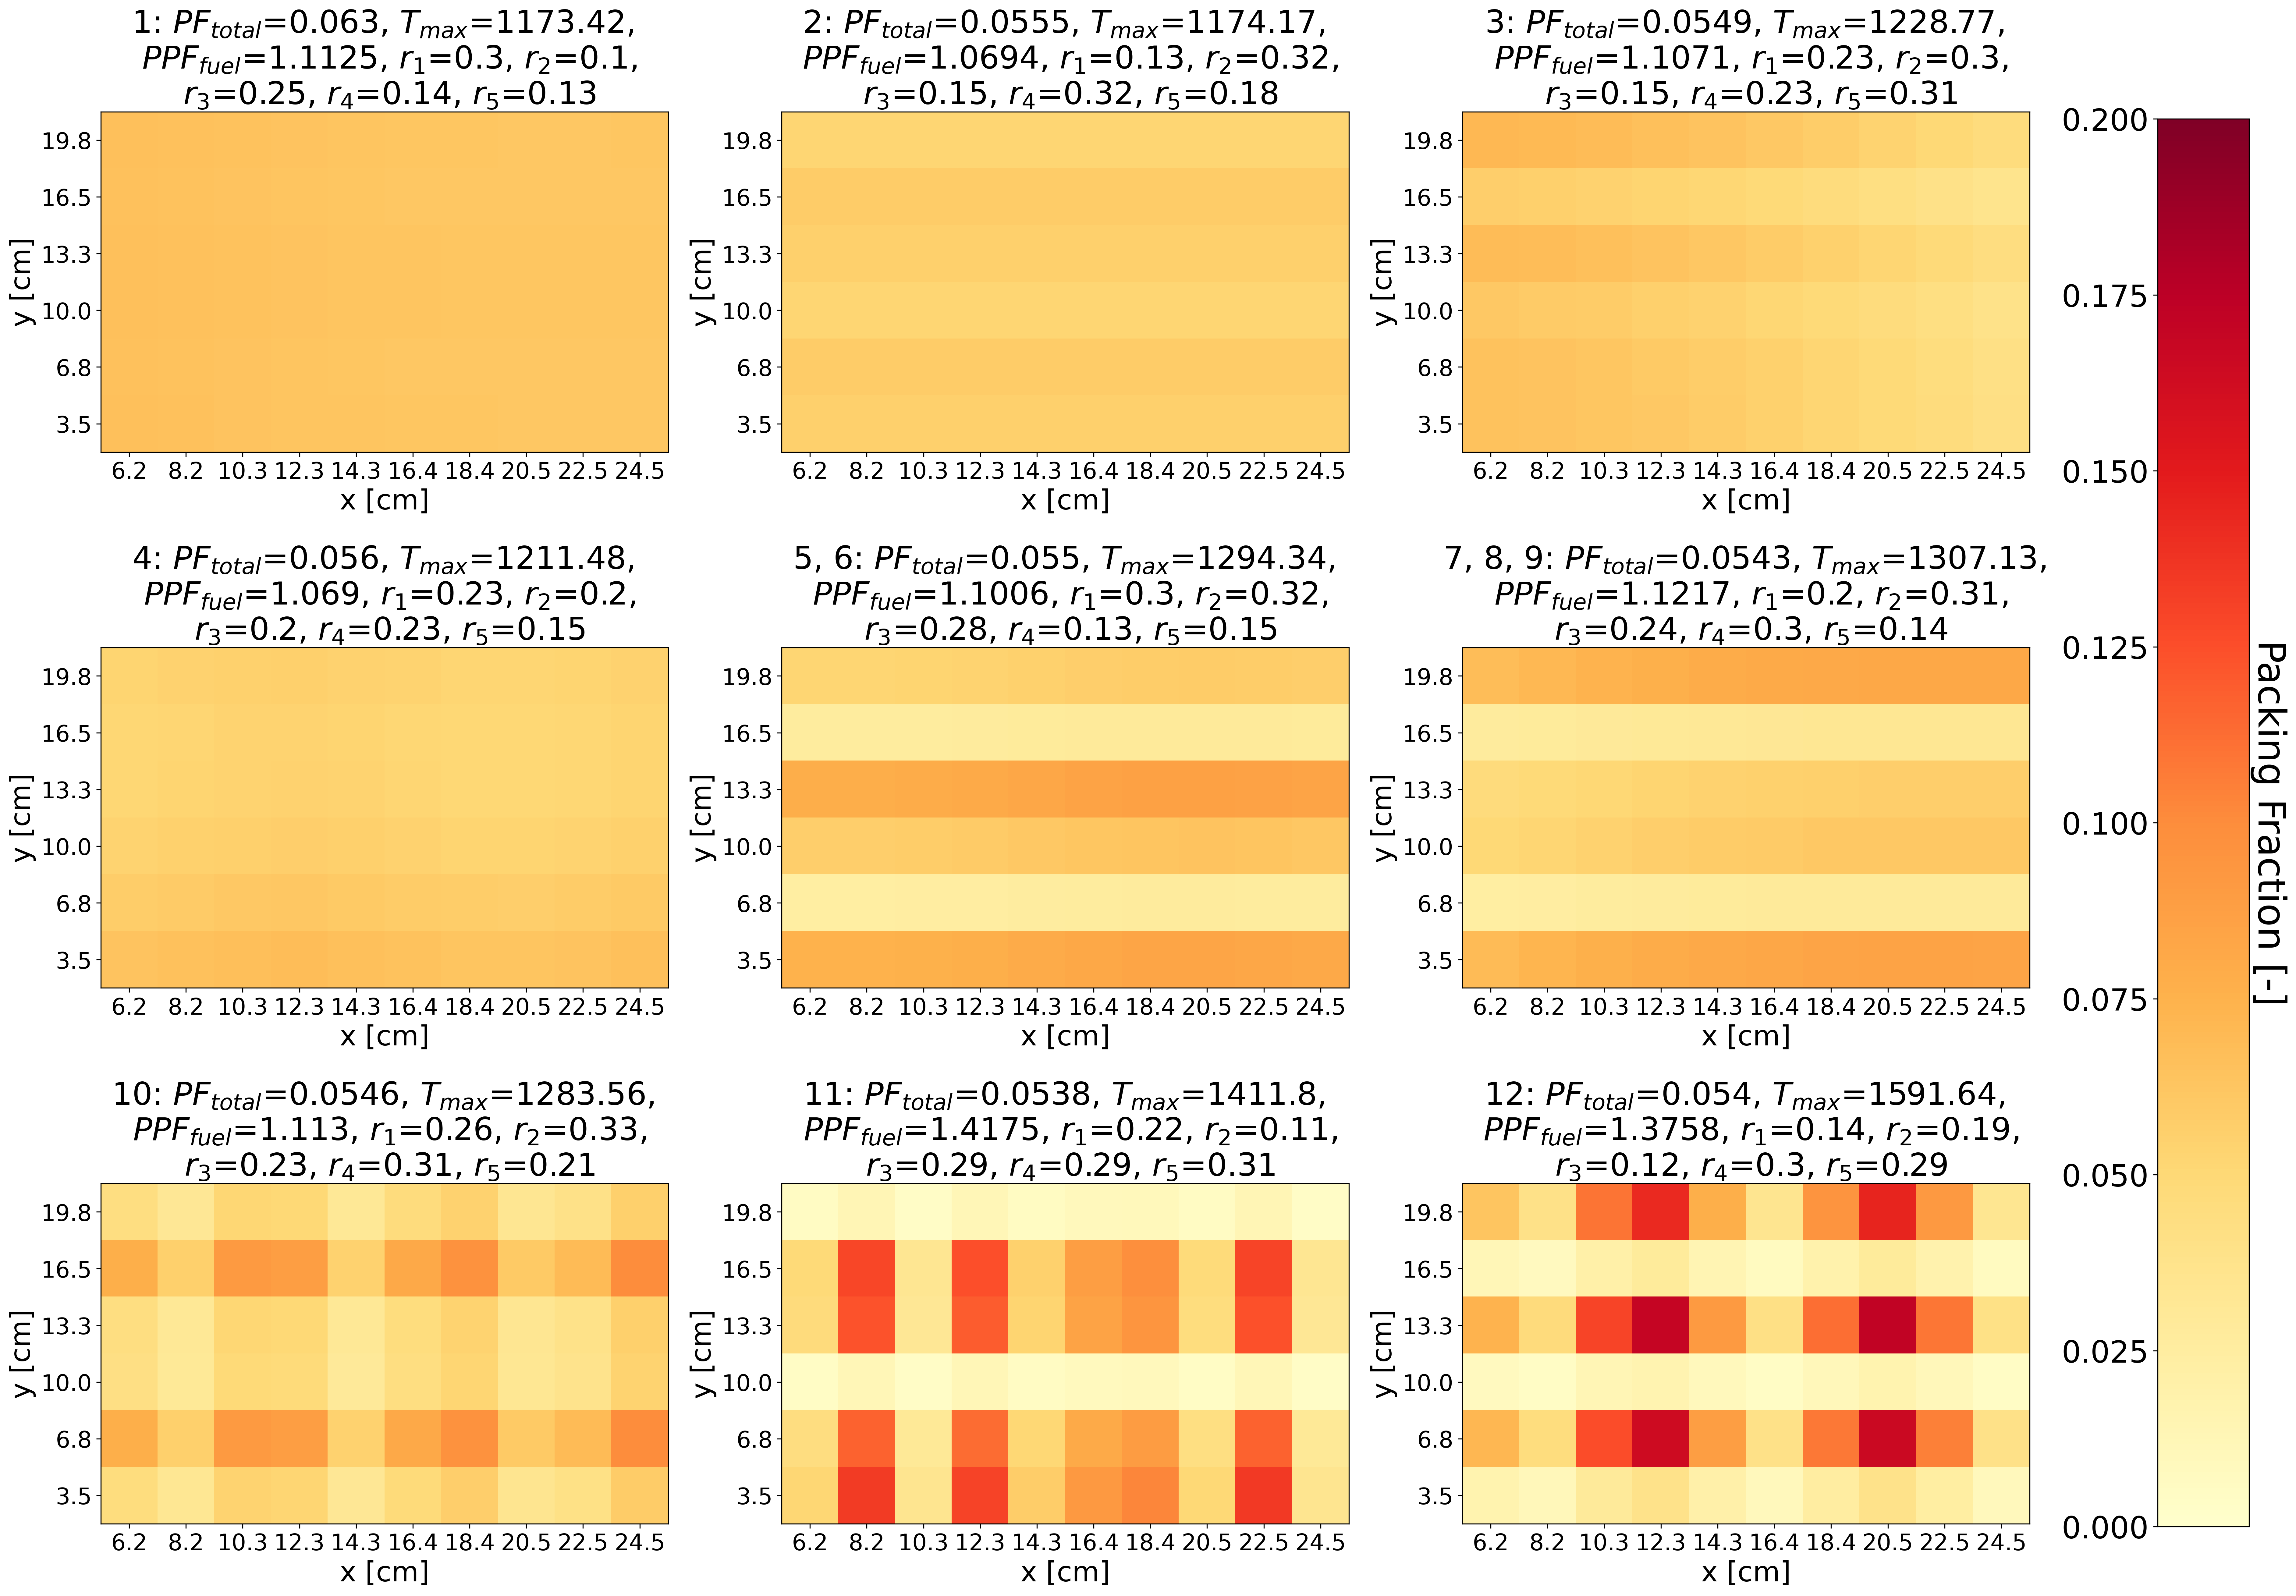
\includegraphics[width=0.7\linewidth]{../docs/figures/assem-obj-3-all-distr.png}}
        \only<2>{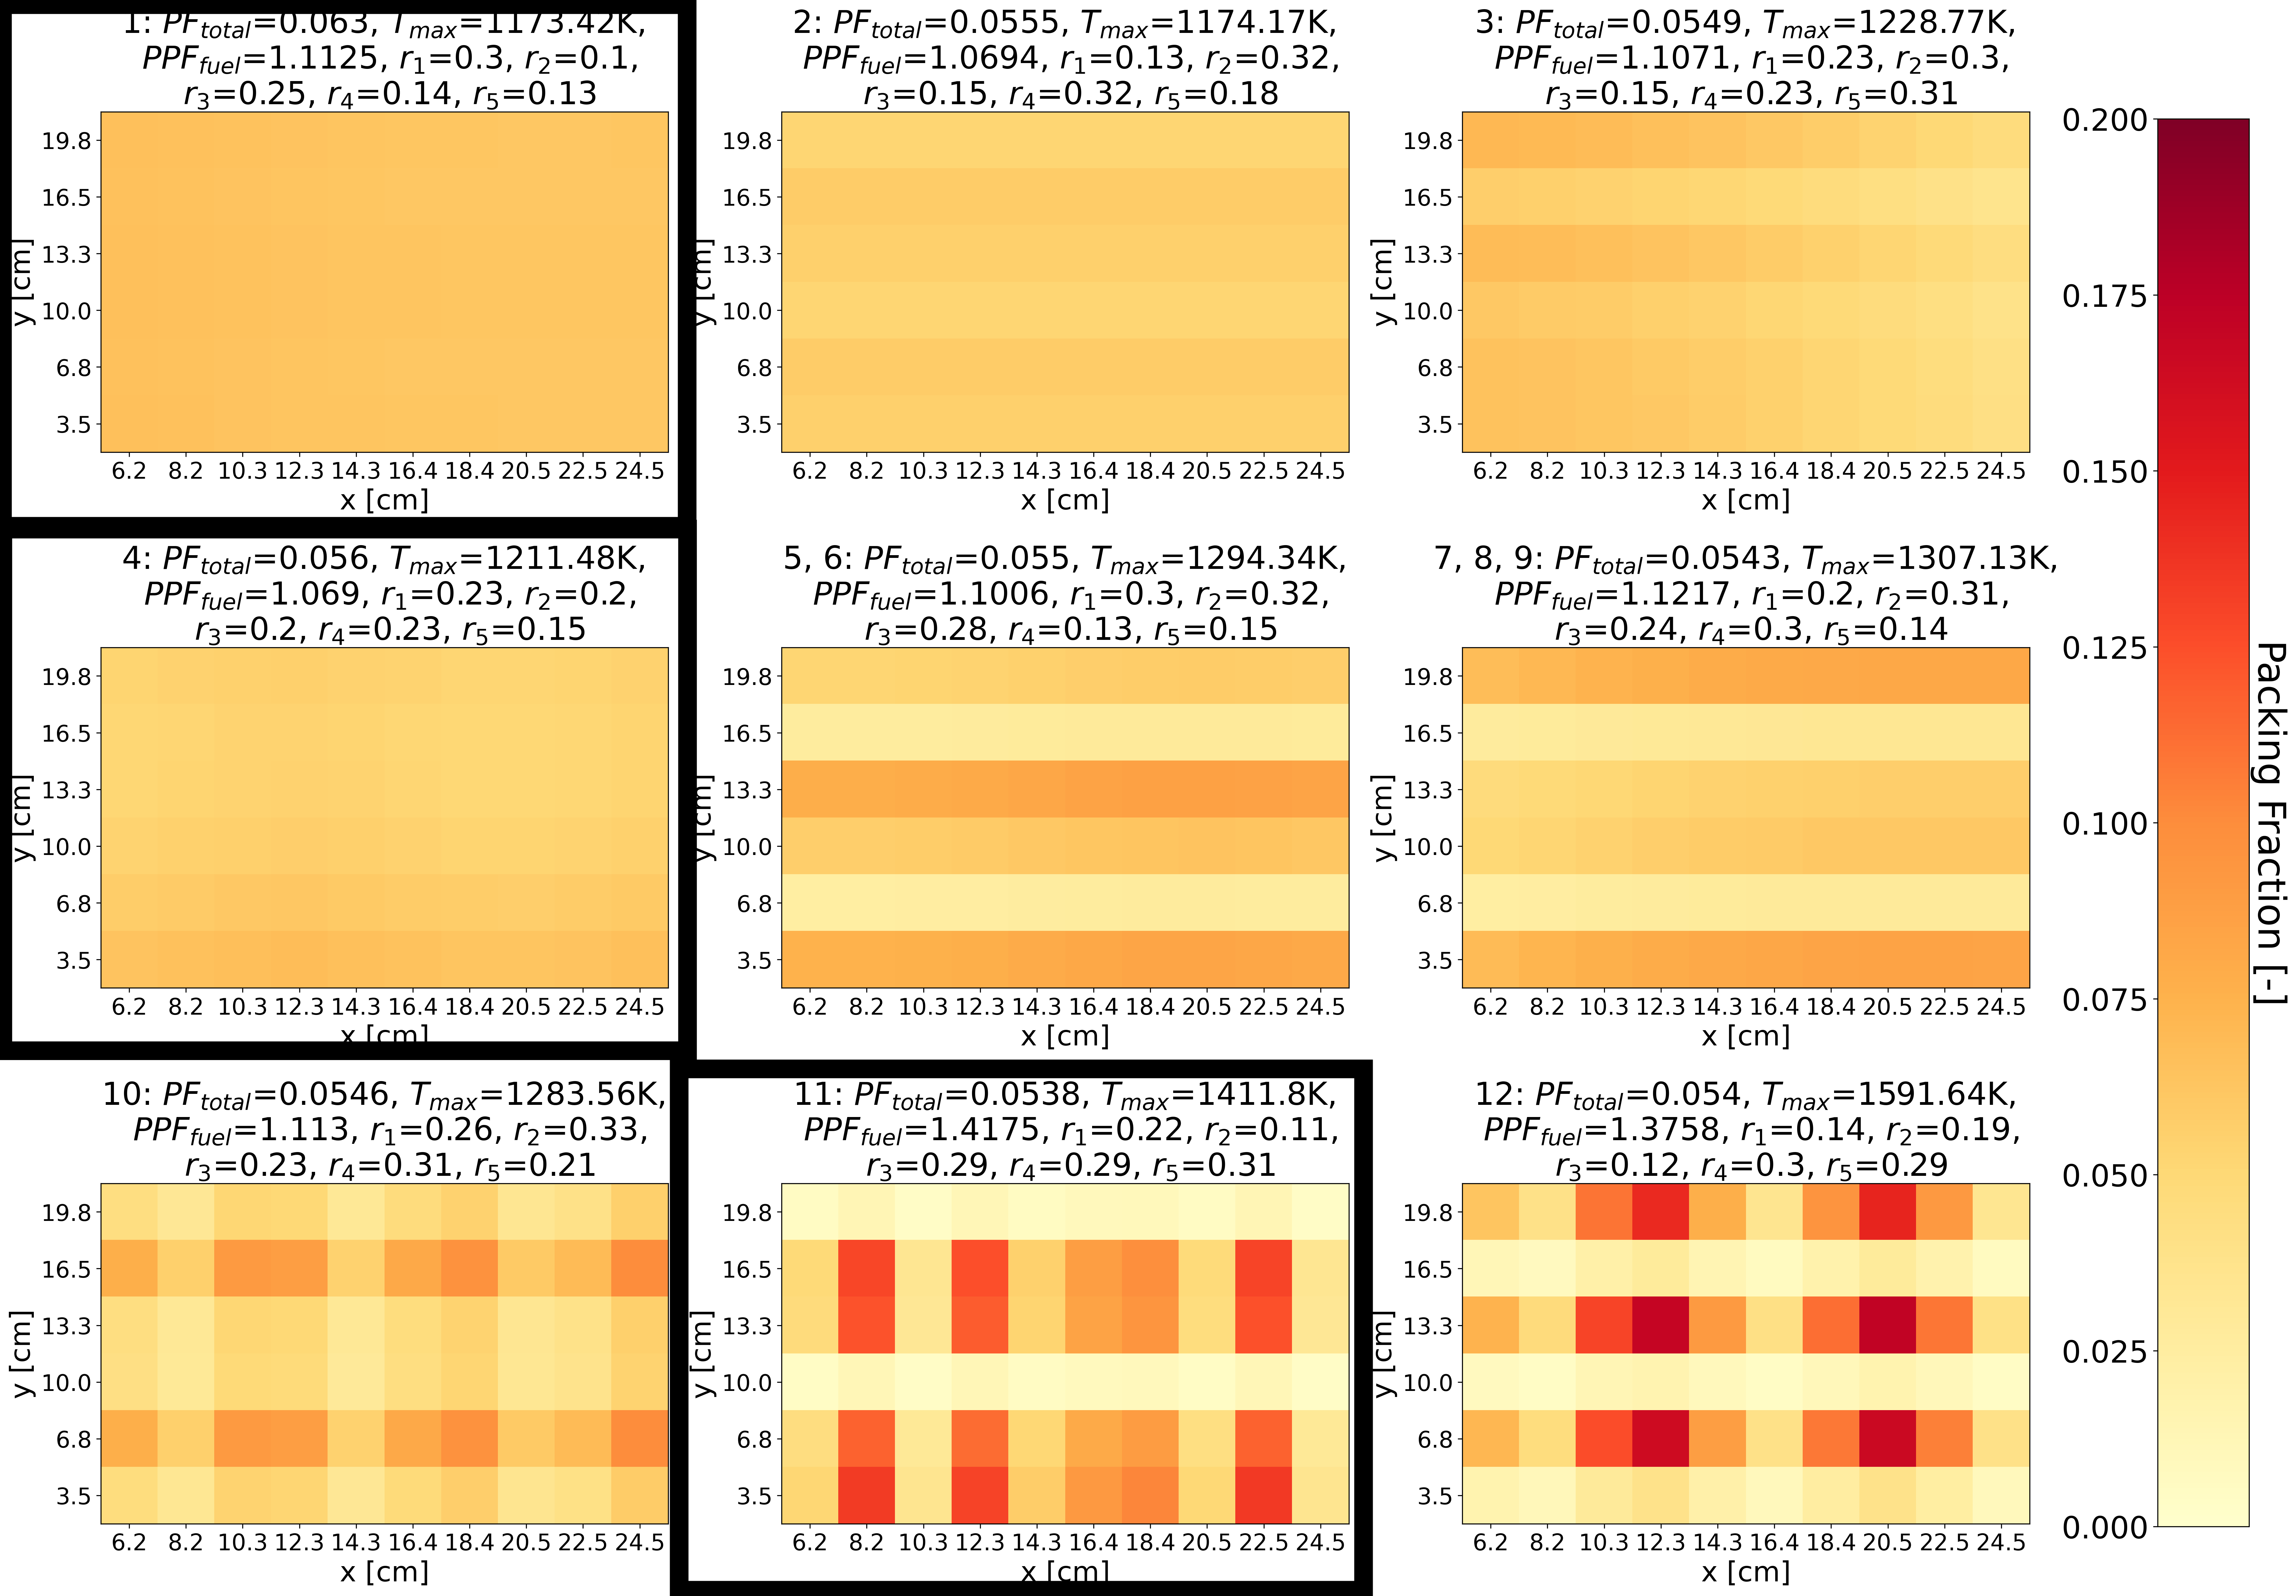
\includegraphics[width=0.7\linewidth]{figures/assem-obj-3-all-distr-annotated.png}}  
    \end{figure}
\end{frame}

\begin{frame}
    \frametitle{AHTR One-Third Assembly Simulation a-3b Results}
    \begin{columns}
        \begin{column}{0.6\textwidth}
        \begin{figure}
            \only<1,4>{\includegraphics[width=\linewidth]{figures/a-3b-four-disr.png}} 
            \only<2>{\includegraphics[width=\linewidth]{figures/a-3b-four-disr-annotated1.png}} 
            \only<3>{\includegraphics[width=\linewidth]{figures/a-3b-four-disr-annotated2.png}} 
        \end{figure}
        \end{column}
        \begin{column}{0.4\textwidth}
            \textbf{Key Observations}
            \begin{itemize}
                \visible<2->{\item TRISO distribution flatness is influenced by minimize $T_{max}$
                objective} 
                \visible<3->{\item Variations in TRISO distributions are influenced by minimize 
                $PF_{total}$ and $PPF_{fuel}$ objectives} 
                \visible<4->{\item Larger radius values are observed near temperature peaks} 
            \end{itemize}
        \end{column}
        \end{columns}
\end{frame}

\begin{frame}
    \frametitle{AHTR One-Third Assembly Simulation a-3b Results}
    \textbf{Simulation a-3b: One-third assembly model that equally minimized all 
    objectives (reactor model 2).}
    \begin{columns}
        \begin{column}{0.5\textwidth}
            \begin{figure}
                \only<1>{\includegraphics[width=\linewidth]{figures/a-3b-equal.png}}
                \only<2>{\makebox[\textwidth][c]{\includegraphics[width=1.1\linewidth]{figures/a-3b-temp.png}}}
            \end{figure}
        \end{column}
        \begin{column}{0.5\textwidth}
            \begin{figure}
                \makebox[\textwidth][c]{
                    \includegraphics[width=1.1\linewidth]{../docs/figures/assem-obj-3-all-min-all.png}} 
            \end{figure}
        \end{column}
    \end{columns}
\end{frame}

\begin{frame}
    \frametitle{Multi-Objective Optimization Major Takeaways}
    \visible<1->{The multi-objective optimization simulations successfully explored the large 
    design space by finding \textbf{wide spread of reactor models on their 
    Pareto fronts}.} 

    \vspace{0.2cm}
    \visible<2->{The reactor models on the Pareto fronts have \textbf{different $PF_{total}$, 
    TRISO distributions, and coolant channel shapes}, depending on the extent 
    each objective is minimized due to the nature of multi-objective
    optimization that results in a \textbf{tradeoff between objectives}.} 

    \vspace{0.3cm}
    \visible<3->{\textbf{Minimize $T_{max}$ objective} 
    \begin{itemize}
        \item Continues to flatten TRISO distribution 
        \item Maximize radius values of FliBe channels located near temperature peaks
        \item TRISO distribution has a larger impact on $T_{max}$ than coolant channel 
        shape  
    \end{itemize}}

    \visible<4->{\textbf{Minimize $PF_{total}$ and $PPF_{fuel}$ objectives} 
    \begin{itemize}
    \item Influences variation in TRISO spatial distributions
    \item These two objectives influence each other to have unexpected TRISO
    distributions at different $PF_{total}$ values
    \end{itemize}}

\end{frame}

\begin{frame}
    \frametitle{ROLLO Tool + AHTR Optimization Simulations: Summary}
    \visible<1->{\begin{block}{I Successfully Completed AHTR Optimization for Non-conventional Designs
    Research Objectives}
    \begin{itemize}
        \item I developed \acrfull{ROLLO} tool that enables generative reactor design
        optimization with evolutionary algorithms 
        \item I demonstrated ROLLO's application on AHTR optimization for spatially variant 
        fuel distributions and wavy coolant channels
    \end{itemize}    
    \end{block}}
    \visible<2->{\begin{block}{Major Takeaways}
        \begin{itemize}
            \item Results demonstrate ROLLO's success in conducting a multi-objective 
            global search of the large AHTR design space to find optimal reactor models 
            that satisfy all the objectives
            \item Once the ROLLO search is complete, reactor designers gain a better 
            intuition of the model's reactor physics and can view the narrower reactor 
            design space that meets their defined objectives
        \end{itemize}
    \end{block}}
\end{frame}

\section{Conclusion}
\chapter{Conclusions and Future Work}
\glsresetall
\label{chap:concl}

Additive manufacturing of reactor core components removes the geometric constraints
required by conventional manufacturing, such as slabs as fuel planks, cylinders as 
fuel rods, etc, enabling further optimization and improvement of core geometries. 
Wide-spread adoption of additive manufacturing methods in the nuclear industry
could drastically reduce fabrication costs and deployment timelines, and improve 
reactor safety. 
Fully benefitting from the new ability to 3D print reactor components requires further 
research into reactor generative design optimization. 
This dissertation explores the new design space enabled by additive manufacturing 
by designing and applying the flexible and open-source \gls{ROLLO} tool to optimize 
the \gls{AHTR} for non-conventional geometries and parameters. 
I successfully explored the \gls{AHTR}'s arbitrary geometry design space by completing 
these three dissertation objectives: 
\begin{enumerate}
    \item I furthered our understanding of the \gls{AHTR} design's complexities 
    through neutronics and thermal-hydraulics modeling by participating in the 
    \gls{OECD} \gls{NEA} \gls{FHR} benchmark.
    \item I developed the open-source \gls{ROLLO} tool that enables generative reactor 
    design using evolutionary algorithm optimization for non-conventional reactor 
    geometries and fuel distributions.
    \item I applied \gls{ROLLO} to conduct generative \gls{AHTR} design.
    \gls{ROLLO} generated \gls{AHTR} designs with varying fuel amounts, fuel 
    distributions, and coolant channel shapes that optimize for three key reactor 
    performance metrics: minimize total fuel amount, maximize heat transfer, and 
    minimize power peaking.
\end{enumerate}
Chapter \ref{chap:fhr-benchmark} addressed objective 1, chapter \ref{chap:rollo} 
addressed objective 2, and chapters \ref{chap:method}, \ref{chap:ahtr-plank-opt-results}, 
and \ref{chap:ahtr-assem-opt-results} addressed objective 3. 

Chapter \ref{chap:fhr-benchmark} reported the \gls{FHR} benchmark Phase I-A and I-B 
results, highlighting the \gls{AHTR}'s passive safety behavior with 
negative temperature coefficients. 
Comparison of $k_{eff}$ results between the reference case and the \gls{AHTR} 
configuration with high heavy metal loading demonstrated that increased fuel 
packing does not always correspond with increased $k_{eff}$ due to self-shielding 
effects.
Chapter \ref{chap:fhr-benchmark} also reported the results of the \gls{AHTR} full 
assembly multiphysics model. The temperature distribution peaked in the fuel stripes near 
the spacers, highlighting to reactor designers that spacer material and location in the 
\gls{AHTR} geometry impact temperature peaks.  

Chapter \ref{chap:rollo} described the \gls{ROLLO} tool developed for this 
dissertation. 
\gls{ROLLO} is a Python package that applies evolutionary algorithm 
optimization techniques to generate nuclear reactor designs that meet user-defined 
objectives and constraints based on user-defined input value ranges. 
\gls{ROLLO} enables reactor designers to optimize any reactor model using robust 
evolutionary algorithm methods without going through the cumbersome process of setting up 
an evolutionary algorithm framework, selecting appropriate hyperparameters, and 
setting up parallelization.
\gls{ROLLO} is effective, flexible, open-source, parallel, reproducible, usable, and 
hosted on Github \cite{chee_rollo_2021}. 

% add more description to contextualize more so that the conclusion can stand on its own
Chapter \ref{chap:method} described the modeling and optimization methodology of the 
\gls{AHTR} plank and one-third assembly optimization conducted using the \gls{ROLLO} 
software.
I varied the following \gls{AHTR} plank and one-third assembly input parameters: 
\gls{TRISO} packing fraction distribution ($\rho_{TRISO}(\vec{r})$), total fuel 
packing fraction ($PF_{total}$), and coolant channel shape; in an effort to minimize 
the following objectives: total fuel packing fraction ($PF_{total}$), maximum 
temperature ($T_{max}$), and fuel-normalized power peaking factor ($PPF_{fuel}$). 

Chapter \ref{chap:ahtr-plank-opt-results} reported the \gls{AHTR} plank's 
\gls{ROLLO} optimization results.
I characterized each objective's driving factors and relationship 
with each input parameter from the results. 
I determined that the minimize $PF_{total}$ objective is driven by maximizing the plank's 
total fission reaction rate and influences oscillations in the TRISO distribution to 
achieve the objective. 
I determined that the minimize $PPF_{fuel}$ objective is driven by flattening the plank's
thermal flux distribution and influences $PF_{total}$ and oscillations in the TRISO 
distribution to achieve the objective.
I determined that the minimize $T_{max}$ objective flattens TRISO distribution and 
maximizes coolant channel shape's radius values to achieve the objective.
Characterizations of each objective for the simple \gls{AHTR} plank model provided 
insights for Chapter \ref{chap:ahtr-assem-opt-results}'s multi-objective 
optimization for the more complex \gls{AHTR} one-third assembly model. 

Chapter \ref{chap:ahtr-assem-opt-results} reported the \gls{AHTR} one-third assembly's
\gls{ROLLO} optimization results.
I verified that the one-third assembly objectives follows the same driving 
factors as the \gls{AHTR} plank optimization objectives. 
The results demonstrated that the minimize $PF_{total}$ objective's driving factor 
maximize total fission reaction rate and minimize $PPF_{fuel}$ objective's driving 
factor flattening thermal flux distribution influenced each other resulting in unexpected 
TRISO distributions at different $PF_{total}$ values. 
Further optimization of the \gls{AHTR} design will benefit from awareness 
of the objectives' relationship. 
The results also demonstrated that the coolant channel shape variation did 
not have as high of an impact on $T_{max}$ as \gls{TRISO} distribution variation.
Simulation a-3b-256's multi-objective optimization showed the result of minimizing all 
three objectives ($PF_{total}$, $T_{max}$, and $PPF_{fuel}$) while varying 
all the input parameters ($PF_{total}$, TRISO distribution, and coolant channel shape).
Figure \ref{fig:assem-obj-3-all-256} showed the 38 reactor models on simulation 
a-3b-256's Pareto front that met all three objectives. 
The reactor models on the Pareto Front have different $PF_{total}$, TRISO distributions, 
and coolant channel shapes, depending on the extent each objective is minimized due 
to the nature of multi-objective optimization that results in a tradeoff between 
objectives. 
These results demonstrate that the generative design optimization process with \gls{ROLLO}
provides the reactor designer with a set of equally good reactor models. 
From this point, it is up to the reactor designer to determine the importance of each 
objective for their purposes, then conduct further sensitivity analysis and 
use higher fidelity models to study the optimal design space before selecting 
the final reactor model.

Chapters \ref{chap:ahtr-plank-opt-results} and \ref{chap:ahtr-assem-opt-results} 
demonstrated \gls{ROLLO}'s success in conducting multi-objective generative reactor 
design optimization. 
\gls{ROLLO} conducted a global search of the large reactor design space and successfully 
generated optimal reactor models on the Pareto front that satisfy all the objectives. 
\gls{ROLLO} also showed how sensitive each input parameter is in relation to 
the objectives. 
Once the \gls{ROLLO} search is complete, reactor designers gain a better intuition of 
the model's reactor physics and can view the narrower reactor design space that meets 
their defined objectives.   

\section{Future Work}
This dissertation's generative design optimization of the \gls{AHTR} model used sine 
distribution variations to govern the \gls{TRISO} packing fraction distribution and  
varied cylinder radius' to generate varying sinusoidal-like pattern coolant channel 
shapes. 
These input parameter variations are only one way to represent the \gls{AHTR} 
geometry. 
There are many other ways to represent the geometry that might give \gls{ROLLO} more 
freedom to explore a larger design space and generate more optimized designs. 
Future reactor designers could consider topology optimization to optimize coolant 
channel shape further.
The major limitation is the computational cost of modeling fluid flow in complex 
coolant channel designs. 

This dissertation demonstrated \gls{ROLLO}'s success in conducting multi-objective 
generative reactor design optimization. 
\gls{ROLLO} can be easily used to optimize any reactor type for any perceivable 
arbitrary input parameters. 
As additive manufacturing technology advances and the \gls{TCR} program 
demonstrates the first 3D printed operational reactor, more reactor designers 
will begin to explore the vast design space enabled by 3D printing. 
Future work includes utilizing \gls{ROLLO} to optimize other reactor types. 
By designing the \gls{ROLLO} tool and demonstrating its success in further optimization 
of the \gls{AHTR} beyond classical input parameters, this dissertation contributes to 
improving reactor technology to ensure that nuclear energy continues to provide 
low-carbon electricity worldwide.


\appendix

\begin{frame}[allowframebreaks]
  \frametitle{References}
  \bibliographystyle{../docs/ieeetran}
  {\footnotesize \bibliography{../docs/2022-chee-dissertation.bib} }

\end{frame}

\section*{Summary}
\begin{frame}
    \frametitle{Summary}
    \textbf{Additive manufacturing could radically transform reactor design.}
    \begin{block}{Research Objectives: AHTR Model Development}
        \begin{itemize}
            \item Further our understanding of the AHTR design's complexities 
            through neutronics and thermal-hydraulics modeling
            \item Participate in the OECD-NEA's FHR Benchmark
        \end{itemize}
    \end{block}

    \begin{block}{Research Objectives: Reactor optimization for non-conventional designs}
        \begin{itemize}
            \item Develop a tool that applies evolutionary algorithms with established 
            nuclear software to optimize reactor design
            \item Demonstrate successful implementation of the optimization tool 
            with OpenMC for single and multi-objective AHTR optimization of 
            non-conventional geometries and fuel distribution
        \end{itemize}
    \end{block}
\end{frame}

\section*{Appendix}
\subsection*{Grad School Journey}
\begin{frame}
    \frametitle{Grad School Journey}
    \vspace{-0.2cm}
    \begin{figure}[]
        \includegraphics[width=0.9\linewidth]{figures/grad-school-journey.png} 
    \end{figure}
\end{frame}

\subsection*{Summary}
\begin{frame}
    \frametitle{Summary}
    \begin{columns}[t]
        \begin{column}{0.5\linewidth}
            \begin{block}{AHTR Model Development for the FHR Benchmark}
                \textbf{Results Presented} 
                \begin{itemize}
                    \item FHR benchmark Phase I-A and I-B results
                    \item AHTR full assembly temperature model 
                \end{itemize}

                Through participation in the FHR benchmark, this dissertation contributes to 
                \textbf{deepening our understanding of the promising \gls{AHTR} technology}.
            \end{block}
        \end{column}
        \begin{column}{0.5\linewidth}
            \begin{block}{ROLLO Tool Development and AHTR Non-Conventional Design Optimization}
                \textbf{Results Presented}
                \begin{itemize}
                    \item \acrfull{ROLLO} tool 
                    \item AHTR Optimization for heterogeneous fuel distributions and wavy 
                    coolant channels 
                \end{itemize}
                
                By designing the ROLLO tool and demonstrating its success in 
                optimization of the \gls{AHTR} beyond classical input parameters, this dissertation 
                contributes to \textbf{optimization tool development for reactors of the future}.
            \end{block}
        \end{column}
    \end{columns}
\end{frame}

\subsection*{FHR Benchmark Specifications}
\begin{frame}
    \frametitle{FHR Benchmark Specifications}
    UIUC participates in the benchmark with OpenMC and using the ENDF/B-VII.1 material 
    cross section library
    \vspace{-0.2cm}
    \begin{table}
        \caption{OECD NEA's FHR Benchmark Phases 
        \cite{petrovic_benchmark_2021}.}
        \vspace{-0.25cm}
        \includegraphics[width=0.7\linewidth]{figures/benchmark-phases.png} 
    \end{table}
    \vspace{-0.3cm}
    \begin{figure}[]
        \includegraphics[width=0.27\linewidth]{../docs/figures/ahtr-fuel-element.png} 
        \vspace{-0.2cm}
        \caption{AHTR fuel assembly.}
    \end{figure}
\end{frame}

\begin{frame}
    \frametitle{FHR Benchmark Specifications}
    Only Phase I-A and I-B specifications have been released 
    \begin{table}
        \caption{Description of the \acrlong{FHR} benchmark Phase I-A cases 
        \vspace{-0.25cm}
        \cite{petrovic_benchmark_2021}.}
        \includegraphics[width=0.6\linewidth]{figures/benchmark-cases.png} 
    \end{table}
    Benchmark participants must produce the following results for 
    the 9 cases: $k_{eff}$, reactivity coefficients ($\beta_{eff}$, 
    $\alpha_D$, $\alpha_{T, FliBe}$, $\alpha_M$), fission source distribution, 
    neutron flux distribution, fuel assembly averaged neutron spectrum
\end{frame}

\subsection*{Key Neutronics Parameters Verification}
\begin{frame}
    \frametitle{AHTR Temp Model $k_{eff}$ and Reactivity Coefficients Verification}
        \begin{table}
            \caption{$k_{eff}$ and reactivity comparison.}
            \vspace{-0.2cm}
            \includegraphics[width=0.9\linewidth]{figures/benchmark-keff.png}
        \end{table}
        The 13pcm $k_{eff}$ and 6pcm reactivity diff, between
        continuous and homogenized OpenMC simulations are within uncertainty, showing 
        that \textbf{selected spatial homogenizations and energy discretizations are 
        acceptable.}
        The Moltres simulation shows a 423pcm diff in $k_{eff}$ and 216pcm 
        diff in reactivity.
        \begin{table}
            \caption{Reactivity coefficients comparison.}
            \includegraphics[width=0.85\linewidth]{figures/benchmark-coeff.png}
        \end{table}
        \textbf{Good agreement} for Moltres' delayed neutron fraction ($\beta_{eff}$) and 
        temperature reactivity feedback ($\frac{\Delta \rho}{\Delta T}$)
\end{frame}

\begin{frame}
    \frametitle{AHTR Temp Model Flux Verification}
    \begin{columns}
    \begin{column}{0.7\textwidth}
    \begin{figure}[]
        \centering
        \includegraphics[width=\linewidth]{figures/benchmark-flux.png} 
        \caption{4-group flux distribution comparison.}
    \end{figure}
    \end{column}
    \begin{column}{0.3\textwidth}
        2-norm Diff [\%]
        \begin{itemize}
            \item Group 1: 0.13\% 
            \item Group 2: 0.08\% 
            \item Group 3: 0.10\% 
            \item Group 4: 0.09\%
        \end{itemize}
        Max Diff [\%]
        \begin{itemize}
            \item Group 1: -10.57\% 
            \item Group 2: +7.58\% 
            \item Group 3: +8.96\% 
            \item Group 4: +6.97\%
        \end{itemize}
    \end{column}
    \end{columns}
\end{frame}

\begin{frame}
    \frametitle{AHTR Temp Model Neutron Energy Spectrum Verification}
            \begin{figure}[]
                \centering
                \includegraphics[width=0.75\linewidth]{figures/benchmark-spectrum.png} 
                \caption{Neutron Energy Spectrum Comparison.}
            \end{figure}
        \textbf{Good agreement} between OpenMC and Moltres models 4-group spectrums.
\end{frame}

\subsection{TRISO Particle Homogenization}
\begin{frame}
    \frametitle{TRISO Particle Homogenization}
    \begin{table}
        \caption{Straightened \acrfull{AHTR} fuel plank $k_{eff}$ for the case with 
        no \gls{TRISO} homogenization and case with homogenization of the four outer 
        layers. Both simulations were run on one BlueWaters supercomputer XE Node 
        using OpenMC with 80 active 
        cycles, 20 inactive cycles, and 8000 particles.}
        \includegraphics[width=0.75\linewidth]{figures/triso-homogenization.png} 
    \end{table}

    The \gls{TRISO} particle outer four-layer homogenization resulted in a $30\%$ 
    speed-up without compromising accuracy with $k_{eff}$ values within each 
    other's uncertainty.

    As a result, the homogenized models are used for all subsequent optimization efforts. 

\end{frame}

\subsection{ROLLO Verification}
\begin{frame}
    \frametitle{ROLLO Successfully Verified with $^{239}Pu$ Critical Bare Sphere}
    \begin{figure}
        \includegraphics[width=0.85\linewidth]{../docs/figures/radius-convergence.png} 
        \caption{Results for each generation for \gls{ROLLO}'s genetic algorithm 
        optimization to the find the critical radius of a  $^{239}Pu$ bare sphere.}
    \end{figure}
    \vspace{-0.2cm}
    \textbf{ROLLO successfully finds the critical radius of the $^{239}Pu$ bare sphere 
    to be 4.9856cm.}
\end{frame}

\begin{frame}
    \frametitle{ROLLO $^{239}Pu$ Critical Bare Sphere Input File}
    \begin{figure}
        \includegraphics[width=0.49\linewidth]{figures/rollo-verify-file.png} 
        \includegraphics[width=0.49\linewidth]{figures/rollo-verify-file2.png}
        \caption{ROLLO $^{239}Pu$ Critical Bare Sphere Input File.}
    \end{figure}
\end{frame}

\begin{frame}
    \frametitle{AHTR Plank Geometry}
    A sine distribution governs TRISO packing fraction distribution: 
    \begin{align}
        \rho_{TRISO}(\vec{x}) &= \left(\textbf{a}\cdot sin(\textbf{b}\cdot x + \textbf{c}) + 2\right) \cdot NF \nonumber
    \end{align}
    \begin{figure}
        \includegraphics[width=0.9\linewidth]{../docs/figures/straightened_plank.png} 
        \caption{Straightened AHTR Plank with 10 fuel cells with random TRISO packing.}
    \end{figure}
    $r_{top}$ and $r_{bot}$ control coolant channel shape: 
    \begin{figure}
        \includegraphics[width=\linewidth]{../docs/figures/coolant-channel-shape.png} 
        \caption{AHTR Plank with coolant channel shape variation, $r_{top}$ = 0.2cm and 
        $r_{bot}$ = 0.3cm.}
    \end{figure}
\end{frame}

\begin{frame}
    \frametitle{Simulation a-3b hypervolume}
    \begin{table}
        \caption{Simulation a-3b hypervolume values at each generation.}
        \includegraphics[width=0.4\linewidth]{figures/a-3b-hypervolume.png} 
    \end{table}

    For each optimization simulation, I must balance convergence and computational cost.

    The hypervolume is calculated by finding the volume between the reference point and 
    the objective values of the Pareto front's reactor models (bigger hypervolume = 
    more converged solution).

    I determine if convergence criteria is met by evaluating if the difference between 
    generations' hypervolume values are getting smaller.
\end{frame}

\end{document}



